\documentclass[
 paper=A4,pagesize=automedia,fontsize=12pt,
 BCOR=15mm,DIV=22,
 twoside,headinclude,footinclude=false,
 english,fleqn,             % fleqn = linksbündige Ausrichtung von Formeln
 bibtotocnumbered,          % Literaturverz. im Inhaltsverz. eintragen
 liststotoc,                % Abbildungsverz. im Inhaltsverz. eintragen
 listsleft,                 % Abbildungsverz. an der längsten Nummer ausrichten
 pointlessnumbers,          % kein Punkt nach Überschriftsnummerierung
 cleardoublepage=empty      % Vakatseiten ohne Paginierung
]{scrbook}
\setlength\parindent{0em}

% Kodierung, Schrift und Sprache auswählen
\usepackage[utf8]{inputenc}
\usepackage[T1]{fontenc}
\usepackage[english]{babel}
% damit man Text aus dem PDF korrekt rauskopieren kann
\usepackage{cmap}
% Layout: Kopf-/Fußzeilen, anderthalbfacher Zeilenabstand
\usepackage{scrlayer-scrpage} \pagestyle{scrheadings}
                      \clearscrheadfoot
                      \ihead{\headmark}\ohead{\pagemark}
                      \automark[subsection]{section}
                      \setheadsepline{0.5pt}
\usepackage{setspace} \onehalfspacing
\usepackage{enumitem} \setlist{itemsep=0pt}
\deffootnote{1em}{1em}{\textsuperscript{\thefootnotemark }}
% clickable references
\usepackage{hyperref}
% Grafiken, Tabellen, Mathematikumgebungen
\usepackage[dvipsnames]{xcolor}
\usepackage{graphicx}
\usepackage{svg}
%\hypersetup{
%	colorlinks,
%	linkcolor={PineGreen},
%	citecolor={cyan!80!black},
%	urlcolor={blue!80!black}
%}
\usepackage{wrapfig}
\hypersetup{hidelinks}
\usepackage{tabularx, booktabs, makecell} \renewcommand{\arraystretch}{1.2}
\usepackage{amsmath,amsfonts,amssymb}
% Darstellung von Fließumgebungen
\usepackage{flafter,afterpage}
\usepackage[section]{placeins}
\usepackage[margin=8mm,font=small,labelfont=bf,format=plain]{caption}
\usepackage[margin=8mm,font=small,labelfont=bf,format=plain]{subcaption}
\usepackage{multicol}
\numberwithin{equation}{chapter}
\numberwithin{figure}{chapter}
\numberwithin{table}{chapter}

%%%%%%%%%%%%%%%%%%%%%%%%%%%%%%%%%%%%%%%%%%%%%%%%%%%%%%%%%%%%%%%%%%%%%%%%%%%%%%%%
% Ab hier ist Platz für eigene Ergänzungen (Pakete, Befehle, etc.)

% Dieses Paket liefert den Blindtext, der als Platzhalter in den Beispieldateien steht.
% Das kannst Du also entfernen, wenn Du den Blindtext nicht mehr brauchst.
\usepackage{lipsum}

\begin{document}
	
	
	% Titelpageseite
	\begin{titlepage}
		\begin{tabularx}{\linewidth}{X}
			
\includegraphics[width=6cm]{TU_Logo_SW} \\\hline\hline
			
			\vspace{4.5em}
			
			\begin{singlespace}\begin{center}\bfseries\Huge
					
					KZM on Si(1, 0, 0) Surface
					
			\end{center}\end{singlespace}
			
			\vspace{5.5em}
			
			\begin{singlespace}\begin{center}\large
					Master-Arbeit \\ zur Erlangung des Hochschulgrades \\
					Master of Science \\
					im Master-Studiengang Physik
			\end{center}\end{singlespace}\medskip
			
			\begin{center}vorgelegt von\end{center}
			\begin{center}
				{\large Andreas Weitzel} \\ geboren am 10.08.1999 in Fulda
			\end{center}\medskip
			
			\begin{singlespace}\begin{center}\large
					Institut für Theoretische Physik \\
					Fakultät Physik \\
					Bereich Mathematik und Naturwissenschaften \\
					Technische Universität Dresden \\ 2023
			\end{center}\end{singlespace}
		\end{tabularx}
	\end{titlepage}
	
	
	% Gutachterseite
	\thispagestyle{empty}\vspace*{48em}
	
	Eingereicht am xx.~Monat~20xx\vspace{1.5em}
	\par{\large\begin{tabular}{ll}
			1. Gutachter: & Prof.~Dr.~XX \\
			2. Gutachter: & Prof.~Dr.~YY \\
	\end{tabular}}
	
	
	% Abstractseite
	\newpage
	\begin{center}\large\bfseries Summary\end{center}
	
	
	Abstract \\
	English: \\
	
	\vspace{20em}
	Abstract \\
	Deutsch \\
	
	
	% Inhaltsverzeichnis
	
	%\cleardoublepage
	\tableofcontents
	
	
	
	% Hauptteil
	\frontmatter
	\chapter{Introduction}
	\section{Motivation}
	Silicon has probably shaped our age like no other element and is responsible for large parts of the revolution humanity went through in the last couple of decades. It is a basic building block of our age, which is not without reason sometimes referred to as the silicon age. This is because of silicons semiconducting properties that are made use of in transistors and integrated circuit chips used in all our everyday electronic devices like smartphones and computers. More specific, Silicon is used in wafers, which are substrates for integrated circuits. Integrated circuits are just sets of smaller, basic electronic building blocks like transistors. Processors, GPUs, Random Access Memory
	
	The surface is semiconducting \cite{himpsel1979photoemission, uhrberg1981experimental, handa1989plasma}
	
	
	\chapter{Main Part}
	\section{Theoretical Background}
	\begin{align}
		exp[a \cos(theta)] = exp[a/2 e^[+\i i\theta]] exp[a/2 e^{-\i i\theta}] = \sum_{n,m=0}^\infty (a/2)^n (a/2)^m/[n! m!] e^[\i i (n-m)\theta]
		= \\
		\sum_{N=-\infty}^{+\infty} {\sum_{n,m=0}^\infty (a/2)^n (a/2)^m/[n! m!] \delta_{n-m, N}} e^[\i i N \theta]
		= \sum_{N=-\infty}^{+\infty} BesselI[N, a] e^{\i i N \theta}
	\end{align}
	\subsection{statistical physics}
	\subsubsection{canonical ensemble}
	The canonical ensemble describes the entirety of all similar systems or all realizations of the same system, that is coupled to a bath and able to exchange energy with it. The system is in thermal equilibrium with the bath and so we are able to make some statements about equilibrium properties of the system. A important tool when dealing with the canonical ensemble or statistical physics in general is the partition function.
	
	The partition function can be motivated through multiple ways, but the most common being entropy maximization. The discrete (continuous) canonical partition function is defined as
	\begin{equation}
		Z =	\sum_i e^{-\beta H_i} \qquad \qquad Z =	\frac{1}{h^d} \int e^{-\beta H(q, p)} d^dq d^dp
	\end{equation}
	
	With the partition function we can express multiple things, for example the probability distribution
	\begin{equation}
		\rho_i =	\frac{1}{Z} e^{-\beta H_i} \qquad \qquad \rho(q, p) = \frac{1}{Z} e^{-\beta H(q, p)} \qquad \text{(maybe with $h^d$?)}
	\end{equation}
	or the thermodynamic total energy, which is the expected value or ensemble average
	\begin{equation}
		\langle E \rangle =	- \frac{\partial \ln (Z)}{\partial \beta}
	\end{equation}
	the variance in energy will be:
	\begin{equation}
		(\Delta E)^2 =	\frac{\partial^2 \ln (Z)}{\partial \beta^2}
	\end{equation}
	In general, if we consider a extensive variable X and a intensive variable Y where X and Y form a pair of conjugate variables, the ensemble average for fixed Y will be
	\begin{equation}
		\left\langle X \right\rangle = \pm \frac{\partial \ln Z}{\partial \beta Y}
	\end{equation}
	I think this has to do with the relation for the ising model where
	\begin{equation}
		M =	\frac{\partial f}{\partial h}
	\end{equation}
	(Wikipedia canonical ensemble (german)) Obvioulsy the logarithm of the partition function plays a central role so we define the \textbf{free energy}:
	\begin{equation}
		F =	-k_B T \ln(Z) \qquad \text{and} \qquad f =	\frac{F}{V}
	\end{equation}
	\subsection{Phase Transitions}
	\subsubsection{Basics}
	\textbf{Definition}
	
	Many Systems exhibit a phase transition when changing an external parameter like their Temperature T through a certain critical temperature $T_c$. This usually means, that they transition from a unordered state to a ordered one. The order of the system is described by the \textbf{order parameter} $\Psi$. In the unordered phase, the (time averaged) value of the order parameter is $\left\langle \Psi \right\rangle = 0$, and in the ordered phase $\left\langle \Psi \right\rangle \neq 0$. In simple words, what happens for (classical) phase transitions is: Above the critical Temperature $T > T_c$, the thermal fluctuations of the system are to strong and destroy every order the system wants to establish. Is the system Temperature lowered to the critical point $T = T_c$, the thermal fluctuations and the interaction between microscopic parts of the system are of the same size but we are still in an unordered state. Below the critical temperature ate $T < T_c$, the microscopic interactions gain the upper hand and the system begins to order in a manner that is determined by the nature of the (microscopic) Hamiltonian. In other words, the system wants to minimize its \textbf{free energy} $F =	U - TS$ and above the critical Temperature the term $-TS$ has greater influence, so the System minimizes its free energy by maximizing its \textbf{entropy S}. Below the temperature the contribution of the \textbf{internal energy U} is greater, so that U is minimized. This minimization is usually achieved through some kind of ordering
	\\
	\\
	A system can have many phase-transition driving parameters (like the temperature), that are then also called \textbf{coupling constants}. For classical phase transition those are usually $T$ and pressure $p$. Depending on the coupling constants, the system can be in one or another phase, so that we can draw phase diagrams with transition lines, like the phase diagram of water.
	\\
	\\
	The static (the system is in equilibrium all the time) properties of the System, like the behavior of the order parameter when changing the $T$ or an external driving force, are usually dealt with by statistical physics. A more mathematical definition of phase transitions can be achieved with the free energy (density) of a lattice with $N$ sites which is depending on the coupling constants K:
	\begin{equation}
		f_b\left\lbrace K \right\rbrace = \lim_{N \rightarrow \infty} \frac{F\left\lbrace K \right\rbrace}{N}
	\end{equation}
	The limit $N \rightarrow \infty$ is called the \textbf{thermodynamic limit} and is usually assumed when dealing with phase transitions, even though strictly speaking it is never realized in the real world, but is a good approximation for real life systems.
	
	The regions where $f_b\left\lbrace K \right\rbrace$ is an analytic (no kinks or jumps) function of the coupling constants are to be identified with the \textbf{phases} and the regions between are the \textbf{phase boundaries}.
	\\
	\\
	\textbf{Types of Phase Transitions}
	
	Actually, $f_b\left\lbrace K \right\rbrace$ is continuous everywhere(everytime?), so there are no jumps. But it could have a kink, whisch would be the first type of phase Transition:
	\begin{enumerate}
		\item $\frac{\partial f_b}{\partial K_i}$ are discontinuous at the phase boundary, this is the \textbf{first order phase transition}. Here, $f_b\left\lbrace K \right\rbrace$ has a kink at the phase transition and its derivative jumps.
		\item $\frac{\partial f_b}{\partial K_i}$ are also continuous, but have a kink at the phase boundary, in this case $f_b\left\lbrace K \right\rbrace$ is smooth and we call this kind \textbf{second order phase transition} or better \textbf{continuous phase transition}.
	\end{enumerate}
	Those considerations of $f_b\left\lbrace K \right\rbrace$ are again exactly only true in the thermodynamic limit, which is never obtained. How do we know if this approximation is reliable? Seems that we can do this by introducing the concept of the \textbf{correlation length} $\boldsymbol{\xi}$, which describes the spatial extent of fluctuations in a physical quantity about the average of that quantity, for example density, or in the Silicon-dimer case deviations from the average inclination angle (How is that helping to see if our approximation is valid? probably if system size $ L \gg \xi$). The correlation length depends on the coupling constants and especially on the temperature, \textbf{diverging to infinity at the transition itself}. More on that later? Since $\xi$ cannot exceed the system size $L$, a finite system differs from an ideal infinite system described by $\boldsymbol{\xi}$. Since in my computations we can only look at relatively small systems, those finite size effects could be important for me.
	\newline
	\newline
	\textbf{Models}
	Often phase transitions and systems in statistical mechanics are described by models like the Ising Model, Heisenberg Model, etc. Those Models usually build on a (microscopic) Hamiltonian which describes the interaction of the parts of the system and for which the partition function is exactly computable. Those Models can be a \textbf{benchmark} for my computations. But since the solution methods for Ising, XY, do not generalize well and more complicated systems are still not solved today, i probably won't be able to put up a microscopic Hamiltonian and derive system properties from there. But maybe i can show that the Ising Hamiltonian is some kind of limit of my Hamilton and maybe i can derive a Langevin equation from my Hamiltonian, which wont be a solution for system properties but describes the dynamic evolution of my system. And maybe i can do some RG calculations when i know my Hamiltonian.
	\newline
	\newline
	\textbf{Spontanous Symmetry Breaking}
	
	The ordering of the Order paramter usually means that some kind of symmetry gets broken. For the Ising Model this would for example mean that above the phase transition, the spins are isotropically distributed in space, meaning that the system looks the same no matter from which ''angle'' i look at it. The Ising Model usually satisfies $\mathbb{Z}_2$-Symmetry, meaning that i could flip every spin and my System would still look the same. After the phase Transition, the degenerate equilibrium states are $\left|\uparrow \uparrow \cdot \cdot \cdot \uparrow \right\rangle$ and $\left|\downarrow \downarrow \cdot \cdot \cdot \downarrow \right\rangle$ and a spin flip results in a Transition between those two states. That means the symmetry is broken? Spontaneous means in this case, that i did not change the Hamiltonian of the System, but the System broke the Symmetry by itself just because the Temperature was lowered. The symmetry group that the considered system belongs to is an important factor for the scaling behavior of the system. \\
	
	Symmetry of the Ising Model: One (the?) symmetry of the Ising model is the so called up-down symmetry or \textbf{time-reversal symmetry}. What this Symmetry basically describes is if i have an external field $M$ and a Spin Configuration $\left\lbrace S_i \right\rbrace$, that the $f_b\left\lbrace K \right\rbrace$, $Z$, etc... are the same if i flip all spins and flip the external field. Flipping the external field is basically equivalent to reversing the time (since the trajectories would run backwards and this is as if the field was flipped?). But this symmetry isn't broken after the phase transition i think? So does the Ising Model not exhibit symmetry breaking? (It obviously does, but which symmetry?) \\
	
	I think the symmetry that is broken by the phase transition is the spin-flip symmetry, which is a different thing than the time reversal symmetry. However, i don't know how this behaves if we have an external field which already breaks the spin flip symmetry. It says here, that event though the Hamiltonian is invariant under time-reversal symmetry, the statistical expectation values are not (like the magnetization $M$). But why not? If I time reverse all my spins, I flip the magnetization and in reverse time this would be okay again? Or can i just flip the time once and the resulting $M$ is the M in reversed time? The fact that the Ising model has a discrete symmetry means that the width of the domain walls must be finite (What does this mean? With intermediate states i could tilt every spin only an infinitesimal small bit and never really reach the other end of the domain wall? Thus an infinite width?). In Ising the thickness can only be one lattice unit. \\
	
	Note that the 1D (d=1) Ising Model does not exhibit a ferromagnetic phase transition for $T > 0$ because there is no \textbf{long range order} (no long range interactions? Even not indirect ones?). Whereas for d=2, long range order can exist above $ T = 0$ The dimension \textbf{above which} a given transition occurs for $T > 0$ is referred to as the \textbf{lower critical dimension}. In the thermodynamic limit, the Ising system can lower its free energy by creating a \textbf{domain wall}, since the penalty for short range interaction is just flat $2J$ (Interaction energy), but the released energy in terms of entropy ist $k_B T \ln(N)$ which becomes arbitrarily large in the thermodynamic limit. So the System is instable concerning thermal fluctuations. \\
	
	Besides the Ising Model there is also the Heisenberg model, where the spins can line up in any direction which is in general a more realistic model, but sometimes Interaction between the spins and the lattice prefers a certain axis so that the spins line up with that axis and the Ising model is actually better. \\
	
	The Symmetry of the Heisenberg-Model is the $O(3)$-Symmetry (or even $SO(3)$ ?), meaning that the Hamiltonian is the invariant under the simultaneous rotation in 3 dimensions of all the spins. \textbf{Important:} We look at the rotation of the spins, keeping the lattice fixed! This continous rotational symmetry is spontaneously broken in the state of long range order. If the spins align in a certain direction, i am left with no symmetry transformation that leaves the statistical average values constant? I mean i could rotate the spins around the axis of direction they are pointing in, but does that count? And which symmetry group is that ($O(1)$))? I thought if i break $SO(3)$ i am left with $SO(2)$. Wasn't there a table somewhere in a book that i read? \\
	
	\textbf{Erodicity Breaking} \\
	In statistical mechanics we identify the time average of an observable of one system with the ensemble average (the average over the whole ensemble, meaning many realizations of my system). In other words: that the time integral over the system observable is the same as the integral over the probability for the system to be in a state times the value of the observable in this state (The probability distribution is extracted out of the ensemble). This is the \textbf{ergodic hypothesis}, or in other words, that one System comes arbitrarily close to every possible configuration as $t \rightarrow \infty$. But if we look at phase broken systems in the thermodynamic limit, the lifetime of one of the degenerate ground states will grow to infinity, so the system is effectively trapped in one or the other region of configuration or phase space. This is known as \textbf{ergodicity breaking}. In my words: The time average over the observable wont be the same as the average over the ensemble, since the broken system will have the same magnetization for example for arbitrarily large times. \\
	
	By the way: the configuration space of the broken symmetry has been fragmented into two regions corresponding to negative or positive magnetization. But those states are time-reversed, so there exists a one-to-one mapping from one to another. This mapping is achieved through the same symmetry that was originally spontaneously broken. (My example is the Ising model, we have the ground states $\left|\uparrow \uparrow \cdot \cdot \cdot \uparrow \right\rangle$ and $\left|\downarrow \downarrow \cdot \cdot \cdot \downarrow \right\rangle$ which are converted into one another by appliying the time reverse symmetry). \\
	
	\textbf{Scaling}
	Systems that do phase transitions all inhibit \textbf{scaling}, which means that two quantities of the system depend on each other in a power law fashion. Often these laws can be deduced by \textbf{dimensional analysis}, which describes the principle of deducing the relationship between quantities by looking at the fundamental base quantities that they depend on. Meaning if we look for a quantity $[c] =	LT^{-1}$ with a certain dimension/einheit, and we know that it can only depend on $[a] =	LT^{-2},[b] = T^{-1}$, we might be able to deduct the scaling law by just combining $a, b$ in a way that they yield the needed dimension:
	\begin{equation}
		c \propto \frac{a}{b}
	\end{equation}
	
	important parameters of the System like:
	\begin{itemize}
		\item The Correlation Length $\xi$
		\item the Relaxation Time $\tau$
		\item the order parameter, e.g. $\Psi$
		\item probably some more?
	\end{itemize}
	scale around the phase transition with \textbf{critical exponents} called $\alpha, \beta, \gamma, \delta, \nu, \eta$. Those are not all independent as we will see in the renormalization group calculations. They scale with the \textbf{reduced temperature}
	\begin{equation}
		\epsilon = \frac{T - T_c}{T_c}.
	\end{equation}
	
	
	\textbf{Important:} critical exponents are defined as \textbf{limiting power laws} as we approach the critical temperature $T \rightarrow T_c$:
	\begin{equation}
		f(\epsilon) \sim \epsilon^\gamma \quad \text{means} \quad \gamma =	\lim_{\epsilon \rightarrow 0} \frac{log f(\epsilon)}{log(\epsilon)}
	\end{equation}
	Critical exponents usually describe the leading behavior and there are \textbf{corrections to scaling}. The Correction vanishes for $|\epsilon| \rightarrow 0$, but may still make a significant contribution for small $\epsilon$. They can \textbf{not} be neglected if one wants to get reliable values for the exponents (LOL what is the correction for $\xi$? -> in RG chapter But without corrections my $\nu$ should still be near the theoretical value?). There are also \textbf{constants of proportionality} that have to be considered, for example for the heat capacity $C_V$:
	\begin{equation}
		C_V(\epsilon) =	\begin{cases}
			A \epsilon^{-\alpha} \qquad &t > 0 \\
			A' (-\epsilon)^{-\alpha'} \qquad &t<0
		\end{cases}
	\end{equation}
	Note that $\alpha$ and $\alpha'$ are always \textbf{equal} and \textbf{universal}, but the \textbf{critical amplitudes} are \textbf{not equal} and \textbf{not universal}. However $A /	A'$ is.
	
	By the way, writing $\xi$ the divergence as
	\begin{equation}
		\xi =	f^\pm t^{- \nu}
	\end{equation}
	defines the universal amplitude ratio $\boldsymbol{U_\xi} =	f^+ /	f^-$. The Value for \textbf{2D Ising} would be
	\begin{equation}
		U_\xi \approx 1.95
	\end{equation}
	
	Measureing critical exponents is notoriously difficult for various reasons:
	\begin{enumerate}
		\item Two far away from $T_c$ the analytic background	(corrections) cannot be ignored and subtracting the background requires modelling of it (curve fitting). Or one could eliminate the background by making $\epsilon$ so small that the diverging contribution overwhelms the background.
		\item Close to the critical point, (for me especially) finite size effects of the system cause rounding of the divergence
		\item We don't know a priori the value of $T_c$ and it has, as well as the corrections, to be treated as an adjustable parameter.
		\item Lastly, we don't even know if the data is accurate since as $T \rightarrow T_c$, it takes longer and longer to equilibrate the system because of the \textbf{critical slowing down}.
	\end{enumerate}
	Critical slowing down describes the effect that, as the correlation length diverges, the fluctuating regions of the system get larger and therefore take longer to equilibrate by their equilibration mechanism (for me diffusion?). The manner in which the \textbf{relaxation time} $\tau_k$ of modes with wavenumber k diverges as $T \rightarrow T_c$ is the topic of \textbf{dynamic critical phenomena}. In general, it is found that the relaxation time of the mode with zero wavenumber $\tau_0$ diverges as
	\begin{equation}
		\tau_0 \sim \xi(T)^z
	\end{equation}
	defining the \textbf{dynamic critical exponent z} (Chapter 8). Cited p.134 phase transition book, what are the wavenumbers here? Wavelengths of fluctuations in the order parameter? So $\tau_0$ relaxation time for largest scale fluctuations.
	
	A List of The system parameters and their corresponding scaling:
	
	\begin{itemize}
		\item specific heat: $C \propto \epsilon^{-\alpha}$
		\item order parameter: $\Psi \propto |\epsilon|^\beta$. Order Parameter is assumed to be zero at the phase transition and non zero below the critical point
		\item response function to driving force J: $\frac{d\Psi}{dJ} \propto	\epsilon^{-\gamma}$
		\item Order parameter to driving Force: $J\propto \Psi^\delta$
		\item \textbf{correlation length:} $\xi \propto \epsilon^{-\nu}$
		\item ''size of correlations at the critical point'' (isn't that the correlation length?). Correlation function scales as $ \propto r^{-d + 2 -\eta}$
		\item the relaxation time also diverges:  $\tau \propto \epsilon^{-\mu}$ [Source?]
	\end{itemize}
	
	\subsubsection{Mean-Field-Methods, Landau Methods}
	In Ising, every spin interacts with every other spin through a coupling constant $J_{ij}S_iS_j$, but in the Weiss model of ferromagnetism, each spin interacts with the average magnetic field due to the magnetization of the other spins $\rightarrow$ mean field theory. I think (I would have to verify) another possibility to write down the Ising model in an external field H would be to write
	\begin{equation}
		H_{total}(i) =	H + \sum_{j (\neq i)} J_{ij} \langle S_j \rangle  + \sum_{j\neq i} J_{ij} (S_j - \langle S_j \rangle)
	\end{equation}
	(What does the i mean, is this only for site i?).
	But in the weiss model, the last term, the \textbf{fluctuation} term is ignored. This is the one that contains the most important physics near the critical point. Basically, weiss tried to describe the magnetic spin model with an effective field $H_{eff}$, induced by the magnetic moment of all other spins. Spins on each site then experience the external magnetic field aswell as the field induced by the average magnetization. The average spin on every site is $M$ and so we were able to write the expression above as total field at site i. For nearest neighbor interaction in d dimensions with strength $J$ the total field then becomes
	\begin{equation}
		H_i =	H + 2dJM \qquad \text{with} \qquad \langle S_j \rangle = M
	\end{equation}
	Plugging this in into the known solution (for the partition function) of the Ising model without interaction, we directly get a self consistency equation
	\begin{equation}
		M	=	\tanh\left(\frac{H + 2dJM}{k_BT}\right)
	\end{equation}
	Depending on $T$, this equation has 1 or 3 solutions. Below $T < T_c$ it has three solutions, two with $M	\neq 0$ (spontaneous magnetization). The transition between 1 and three solutions happens at $T_c =	\frac{2dJ}{k_B}$. We can expand the self consistency equation in the vicinity of $T_c$, so for $\tau =	\frac{T_c}{T}$ and for small M, which will yield:
	\begin{equation}
		\frac{H}{k_B T} \approx M (1 - \tau) + M^3\left(\tau - \tau^2 + \frac{\tau^3}{3} + ...\right) +...
	\end{equation}
	This tells us three things: For $H=0$ and first order in $\tau$, we get
	\begin{equation}
		M \approx \sqrt{3} \left(\frac{T_c - T}{T_c}\right)^{\frac{1}{2}} \qquad \text{implying} \qquad \beta = 1/2 + ...
	\end{equation}
	And, at the phase transition, so $\tau =	1$:
	\begin{equation}
		H \sim M^3 \qquad \text{implying} \qquad \delta = 3
	\end{equation}
	Differentiating for $H$ and replacing the derivatives of $M$ with the isothermal magnetic susceptibility $\xi_T =	\frac{\partial M}{\partial H}$ lets us conclude
	\begin{equation}
		\chi_T \sim |T - T_c|^{-\gamma} + ... \qquad \text{implying} \qquad \gamma =	1
	\end{equation}
	So we were able to extract the \textbf{mean field values for the critical exponents} $\beta , \delta$ and $\gamma$, which are $1/2$, 3 and $1$ respectively. We can see that the susceptibility \textbf{diverges}. We could also calculate an result for $\alpha$.
	
	BTW: Those expansions are probably a source for the corrections to scaling that we talked about.
	
	\textbf{spatial correlations}: Mean field and spatial correlations? We don't have fluctuations of the order parameter, but the \textbf{correlation length} also governs the qay in which the order parameter varies in space in response to an \textbf{inhomogeneous external field}. We can express the \textbf{two point correlation function}:
	\begin{equation}
		G(r_i - r_j) =	\langle S_i S_j \rangle - \langle S_i \rangle \langle S_j \rangle
	\end{equation}
	as derivatives of the partition function:
	\begin{equation}
		\sum_{i} \langle S_i \rangle =	\frac{1}{\beta Z} \frac{\partial Z}{\partial H} \quad \text{and} \quad  		\sum_{ij} \langle S_i S_j\rangle =	\frac{1}{\beta^2 Z} \frac{\partial^2 Z}{\partial H^2}
	\end{equation}
	\textbf{Important:} Could you use that to benchmark your simulation for your quadratic interaction model?
	
	We can do the same thing for the isothermic susceptibility
	\begin{equation}
		\chi_T =	\frac{1}{N \beta} \frac{\partial^2 \ln (Z)}{\partial H^2}
	\end{equation}
	Calculations and substituting with the correlation function yields..
	\begin{align}
		\chi_T 	&= \beta \sum_{i}G(\mathbf{x_i}) \\
		&= \frac{\beta}{a^d} \int_\Omega d^d\mathbf{r} G(\mathbf{r})
	\end{align}
	This is known as the \textbf{static susceptibility sum rule}, could you use that to calculate the susceptibility for your system? Or does that only apply to mean field theories?
	
	Since we know now that $\chi$ diverges, the correlation function has to reflect this divergence. We know, but will see later, that
	\begin{equation}
		G(\mathbf{r}) \sim \frac{1}{|\mathbf{r}|^{(d-1) / 2} \xi^{(d-3) / 2}} e^{- |\mathbf{r}| /	\xi}
	\end{equation}
	
	With that we get our important result for the correlation length:
	\begin{equation}
		\xi \sim \left(\frac{T- T_c}{T_c}\right)^{-\nu} \qquad \text{with} \qquad \nu =	\frac{1}{2}
	\end{equation}
	
	\textbf{Landau Theory}
	Hopefully we will show why there is universality and why mean field theory cannot be correct at the critical point in the following.
	
	Can you do a mean field theory calculation for your critical exponents for your	interaction? My Order parameter would be the average displacement in z-Direction or the inclination angle (for the symmetric case) or something like that, just a \textbf{scalar}.
	\begin{equation}
		M =	\frac{1}{N} \sum_i q_i =	\begin{cases}
			0 		\qquad &T > T_c \\
			\neq 0 \qquad &T < T_c
		\end{cases}
	\end{equation}
	(How do i actually know that it is nonzero below $T_c$?, i mean it is logical because the free energy will be minimized by aligning, but how do you actually know? I mean my quadratic interaction can directly be diagonalized to an Interaction $\lambda_k Q_k^2$ which would be like Ising and we could therefore do a mean field calculation analogous to ising? So we would get the ising mean field exponents? And I	mean universality would tell me anyway that we would have the same critical exponents...)
	My Hamiltonian $\mathcal{H} = V_{\text{doulbe well}} + V_{\text{quadratic interaction}}$ is symmetric under the transformation $q_i \rightarrow -q_i$ which would be $\mathbb{Z}_2$? -	Symmetry and we would therefore be Ising-like.
	
	\textbf{universality}
	Landaus thinking was that for Ising and Fluids the critical exponents are the same because their Gibbs free energy had the same form (powers in the order parameter), which led him to propose his \textbf{Landau free energy L}, which depends on the coupling constants $\lbrace K_i \rbrace$ and the order parameter M. The State of the System is determined by the absolute minimum of L with respect to the order parameter. Landau had some constraints for his free energy:
	\begin{enumerate}
		\item L consistent wiht symmetries of system
		\item L should be expandable in powers of M near $T_c$, probably to yield the critical exponents that were obtained during mean field calcs?
		\item L	is a local function, so if the Order parameter fluctuates, the Free energy at one point far enough away from another should not depend on each other?
		\item M =0 solves the minimum equation for L above the critical temperature
	\end{enumerate}
	Often we can eliminate even/uneven powers from symmetry constraints of the system. For Ising universality class, the Landau free energy becomes
	\begin{equation}
		L = a\epsilon M^2 + \frac{1}{2}b M^4 - H M
	\end{equation}
	but in principle, the Landau function is constructed by writing down all possible scalar terms which are powers and products of the order parameter components, consistent with the symmetry requirements of the particular system.
	
	\textbf{critical exponents in Landau:}
	From this Landau Free Energy we get for the Minimum for no external field
	\begin{equation}
		M =	\left(-\frac{a\epsilon}{b}\right)^{\frac{1}{2}} \qquad \text{implying} \qquad \beta =	1/ 2
	\end{equation}
	Allowing external field and minimizing L for it leads to
	\begin{equation}
		a \epsilon M	 + b M^3 =	\frac{1}{2} H \qquad \text{implying} \qquad \delta = 3
	\end{equation}
	Differentiating this again with respect to H yields to the equation for the susceptibility, yielding $\gamma =	1$. We have reproduced or also found the critical exponents that were already introduced by the weiss model
	
	\textbf{Spatial correlations in Landau Model}:
	We now allow $M \rightarrow M(r)$. A spatially varying order parameter can result out of an inhomogenous external field $H(r)$.
	\textbf{Coarse Graining}: We already now that the patches of same spin orientation grow as we approach $T_c$. That suggests that we divide the system into patches of linear dimension $\Lambda^{-1} \approx \xi$ and introduce \textbf{local magnetization} within this block $M_\Lambda(r)$ centered at $r$. We call this $M_\Lambda$ the coarse grained order parameter or in this case the coarse grained magnetization. L cannot be just the sum of the free energy within each patch, because that would mean that there could be large differences in adjacent patches, but that would be energetically unfavorable. Especially since the local magnetization is by construction smoothly varying. Thats why we want to introduce a term that penalize the difference in magnetization between patches. The simplest one would be quadratic in the difference, so we get for L:
	\begin{equation}
		L =	\sum_r \mathcal{L}(M_\Lambda(r)) + \sum_r \sum_\delta \frac{\gamma'}{2} \left(\frac{M_\Lambda(r) - M_\Lambda(r + \delta)}{\Lambda^{-2}}\right)
	\end{equation}
	Or we can rewrite it as an integral using that $M_\Lambda$ is slowly(smoothly?) varying in space (since near the critical point $\xi >> a$):
	\begin{equation}
		L =	\int_\Omega d^d{r} \left[\mathcal{L} (M_\Gamma (r)) + \frac{\gamma'}{2} (\nabla M_\Lambda(r))^2\right]
	\end{equation}
	\textbf{Correlation functions}: For Ising model this L	becomes
	\begin{equation}
		L\lbrace M(r) \rbrace =	\int_\Omega d^d{r} \left[ a\epsilon M^2 + \frac{1}{2}b M^4 - H(r) M(r) + \frac{\gamma'}{2} (\nabla M_\Lambda(r))^2\right]
	\end{equation}
	We will see how to generate correlation functions from the partition function Z:
	\begin{equation}
		Z =	\text{Tr}_{M(r)} e^{-\beta L\lbrace M(r) \rbrace}
	\end{equation}
	The steps are the same like for the Weiss model above and by using the \textbf{continuum limit}, $a \rightarrow 0$, $N \rightarrow \infty$ but $V =	Na^d = const$, we can just take over the results.
	
	For continuous values of the Orderparameter, the trace operation becomes an integral. It is a functional integral, so some math is required to evaluate this. Usually this is done in fourier space.
	
	I think, if we have discrete sites and therefore discrete values for the order parameter $M_i$ and the external field at these sites $H_i$, we can write the partition function as
	\begin{equation}
		Z =	Z\lbrace H_i \rbrace  =	\text{Tr} \exp\left[- \beta \left(H_\Omega - \sum_{i}H_i M_i\right)\right]
	\end{equation}
	And the correlation function can then be written by differentiation
	\begin{equation}
		\langle M_i M_j \rangle = \frac{1}{\beta^2 Z\lbrace H_k \rbrace} \frac{\partial}{\partial H_i} \frac{\partial}{\partial H_j} Z\lbrace H_k \rbrace
	\end{equation}
	In the case of infinite Degrees of freedom, so $M(r)$, we have to replace the partial derivatives with functional derivatives, since the sum in the trace becomes an Integral.
	
	\textbf{Response Functions:} The partition function is in field theories often called the \textbf{generating functional} (for obvious reasons?). We can generate the expectation value of the order parameter and the generalized isothermal susceptibility from the free energy $F\lbrace H(r) \rbrace$:
	\begin{equation}
		\langle M(r) \rangle = - \frac{\partial F}{\partial M(r)} \quad \text{and} \quad \chi_T(r, r') =	- \frac{\delta^2 Z}{\delta H(r) \delta H(r')} = ... =	\beta G(r, r')
	\end{equation}
	For a translationally invariant system
	\begin{equation}
		G(r - r') =	k_B T \chi_T(r - r') \qquad \text{and} \qquad \hat{\chi}_T(k) =	\beta \hat{G}(k)
	\end{equation}
	Which is an example of a principal result of \textbf{linear response theory} which means that the response functions are proportional to correlation functions.
	
	We can now calculate the Correlation function $G(r)$ by minimizing L with respect to the order Parameter $\left(\frac{\delta L}{\delta M(r)} =	0\right)$ and then deriving this equation with respect to H(r') to get an expression for $\chi_T$ which is (in this case /	always?) an expression for G and on the way the correlation lengths in mean field theory above and below $T_c$:
	\begin{equation}
		\xi_<(\epsilon) =	\left(\frac{\gamma'}{2a\epsilon}\right)^{\frac{1}{2}} \qquad \qquad \xi_<(\epsilon) =	\left(- \frac{\gamma'}{4a\epsilon}\right)^{\frac{1}{2}} \quad \text{not sure if 4 and 2 is intended}
	\end{equation}
	$\gamma$ here is the critical exponent, even though i don't really get how it enters the calculation. It suddenly shows up when minimizing L. Or not, it is probably the factor $\gamma'$ from the landau function, i overlooked it last time.
	
	The equation for the Correlation function:
	\begin{equation}
		\left(- \nabla^2 + \xi^{-2}\right) G(r -r') =	\frac{k_B T}{\gamma} \delta(r - r')
	\end{equation}
	Which by the way shows that the two-point correlation function is actually a green function
	Fourier Transforming leads to
	\begin{equation}
		\hat{G}(k) 	=\frac{k_B T}{\gamma} \frac{\xi^2}{1 + k^2 \xi^2(\epsilon)} \qquad \text{and} \qquad \chi_T =	\frac{\xi^2}{\gamma} \qquad \text{not $\hat{\chi}$?}
	\end{equation}
	
	Solving in real space yiels
	\begin{equation}
		\frac{1}{g} G(\rho) =	\begin{cases}
			e^{-\rho} \qquad &d=1 \\
			(2\pi)^{-d/2} \rho^{-(d-2) / 2} K_{(d-2)/2}(\rho) \quad &d \geq 2
		\end{cases}
	\end{equation}
	with
	\begin{equation}
		g =	\frac{k_B T}{\gamma} \xi(\epsilon)^{2-d} \qquad \text{and} \qquad \rho =	r/\xi
	\end{equation}
	$K_{(d-2)/2}(\rho)$ are the modified spherical Bessel functions of the third kind.
	If the Dimension is for the System, which it should be, and not somehow for the Order parameter, it makes sense to fit to the Lorentzian since this has a much more easy form.
	
	And with this we recover in the case of $T \neq T_c, r >> \xi$ and $d \geq 2$:
	\begin{equation}
		G(r) =	\frac{\pi^{(1-d)/2}}{2^{(1+d)/2}} \cdot \frac{k_B T}{\gamma} \cdot \frac{e^{-r/\xi}}{r^{(d-2)/2}} \cdot \frac{1}{\xi^{(d-3)/2}}
	\end{equation}
	Which is an \textbf{important result} since I	use that to calculate the correlation length.
	
	\textbf{Breakdown of Landau-Theory} \\
	Following statements are true for ising universality class.
	Mean field theory fails when our System approaches $T \rightarrow T_c$. The Error for the correlation function for the distance $R$ that we have in the weiss model in comparison with the ising model scales like
	\begin{equation}
		E_R \sim \left(\frac{a}{R}\right)^d
	\end{equation}
	so mean field theory works well when $R/a$ is large or equivalently, when the coordination number is large	(why is that the same?). Mean field theory is exact when all spins couple to all other spins.
	
	\textbf{Important Reminder:} The order parameter and Landau theory itself are defined with respect to a length scale $\Lambda^{-1}$, which is of the order (but not larger than) $\epsilon$.
	
	
	
	We can also derive the \textbf{Ginzburg criterion for phenomenological landau theory}. It is
	\begin{equation}
		|\epsilon|^{(4-d)/2} >> \frac{k_B}{4 \Delta C \xi(1)^d}
	\end{equation}
	With $\Delta C$ being the discontinuoty in the heat capacity.
	This equation is always satisfied fo $d > 4$, so Landau theory gives correct exponents and a good qualitative picture. For $d < 4$ Landua theory fails at the critical point and for $d=4$ it is not quite correct and needs corrections. The dimension above which Landau theory becomes correct is called the \textbf{upper critical dimension}. It can differ from 4 for other universality classes.
	
	Another useful fact: The real $T_c$ at which the phase transition occurs must be lower than the one used by Landau theory, because (somehow) Landau theory neglects long wavelenght fluctuations and those would increase the entropy and therefore the entropy would longer dominate the part of the free energy.
	
	\textbf{Gaussian Approximation:} We calculate the correlation function and then critical exponents again using the gaussian approximation to solve the functional integral in the partition function directly (And not doing it by minimizing L	and using static susceptibility sum rule). We will get the lowest order systematic correction to mean field theory. The gaussian approximation allows \textbf{fluctuations} about the spatially uniform mean field, but assumes that those are distributed normally. The flucuations are then non interacting (obviously, we just stated that they are normally distributed?). Basically the gaussian approximation is an approximation of a functional integral fo a partition or generating function by a product of gaussian integrals and has many applications/counterparts in other areas of physics.
	
	What can be approximated is basically any integral over a distribution $P(q)$ that looks a bit like gauss. And with looks a bit like gauss i mean its \textbf{peak}, has to be sufficiently close to its \textbf{mean} which seems to just be the ginzburg criterion. What we now do is we taylor our Hamiltonian to the second order about the maximum of $P$, $q_0$, which minimizes the free energy, so the first order term in the taylor expansion is zero, and then approximate $P$ with it:
	\begin{equation}
		P(q) \propto e^{-\beta H(q)} \approx e^{-\beta H(q_0) - \frac{1}{2} (q - q_0)^2 / \lambda^2} \quad \text{with} \quad \frac{1}{\lambda^2} =	\beta \frac{\partial^2 H}{\partial q^2}(q_0)
	\end{equation}
	And then Z is just
	\begin{equation}
		Z =	e^{-\beta F} = \int_{\infty}^{\infty} dq e^{-\beta H(q)} =	e^{-\beta H(q_0)} \sqrt{2 \pi \lambda}
	\end{equation}
	\begin{equation}
		F =	H(q_0) - \frac{1}{2} k_B T \ln(2 \pi \lambda^2)
	\end{equation}
	An analog calculation applies for N degrees of freedom, the result is
	\begin{equation}
		F =	H(q_0) -\frac{1}{2} k_B T \sum_{i = 1}^{N}\ln(2\pi \lambda_i^2)
	\end{equation}
	
	For infinite number degrees of freedom we evaluate the functional integral
	\begin{equation}
		Z =	\int \text{D}M e^{-\beta L(\lbrace M(r)\rbrace)}
	\end{equation}
	L as above but added a constant term $a_0 V$. We now find the configuration that minimizes L	above and below $T_c$ respectively and then expand L around it to second order. Integration done in fourier space. Calculation probably not that important. Result is
	\begin{equation}
		F =	a_0 V - \frac{1}{2} k_B T \sum_{|k| < \Lambda}^{} \ln \left(\frac{2 \pi V k_B T}{2at + \gamma k^2}\right)
	\end{equation}
	
	Somehow it seems to be possible to calculate the correlation function directly from the definition instead of minimizing the landau free energy and using the static susceptibility sum rule, but I	don't really get what this has to do with the gaussian approximation. We use the representation of L	in fourier space that we used in the last step but besides from this nothing else. The result found earlier is just confirmed.
	
	Confirming the correlation function (or the fourier transform of it)(critical exponent $\eta =	0$? What was that again?) confirms the susceptibility (critical exponents $\gamma =	1$), which is again connected to the correlation length (critical exponent $\nu =	1/2$), so the only exponent that changes from mean field predictions is the heat capacity exponent $\alpha$
	
	The calculation of the heat capacity per unit volume
	\begin{equation}
		c_V =	- T	\frac{\partial^2 (F/V)}{\partial T^2}
	\end{equation}
	does not yield to much insight. We might note that the diverging contribution comes from the long wavelength behavior of the system ($k \rightarrow 0$). We get
	\begin{equation}
		C \sim \begin{cases}
			\epsilon^{-(2 - d/2)} \qquad &d < 4 \\
			\text{finite} \qquad 	&d > 4
		\end{cases} \qquad \Rightarrow \qquad \alpha =	2 - d/2
	\end{equation}
	We see explicitly that critical behavior depends on the dimension d, but not on the parameters in the landau function.
	\subsubsection{Ginzburg Landau Methods and Time dependant GL}
	\subsubsection{Renormalization Group Methods}
	\label{withoutsecRG}
	Renormalization Group methods allow to study how system behaviour (or not behaviour, general changes) changes when viewed at different scales. The basic idea behind it is to transform length scales in the hamiltonian so long as it changes something one sometime it should converge (scale invariance). This change in scale is called a scale transformation. RG-Methods can be used to deduct the scaling laws and critical exponents.
	\textbf{Dimensionless Analysis and critical exponents}: We can also use the already seen dimensionless analysis to extract some information about the critical exponents.
	Look at the two-point-correlation function:
	\begin{equation}
		G(r - r') =	\left\langle \phi(r) \phi(r')\right\rangle = \int p(\phi) \phi(r) \phi(r') D\phi \quad \Rightarrow \quad [G(r-r')] =	[\phi]^2 =	L^{2-d}
	\end{equation}
	[Why this dimension? source p.193 Lectures on phase...]
	The Fourier-tranform (so the structure factor) then has the dimension
	\begin{equation}
		[\hat{G}(k)] =	L^2
	\end{equation}
	If we do a scale transformation $L \rightarrow L' = \varepsilon L$, then the structure factor should transform like
	\begin{equation}
		\hat{G}'(k') =	\varepsilon^{-2} \hat{G}(k) \qquad \text{because} \quad \hat{G}'L'^2 =	\hat{G}L^2
	\end{equation}
	This is always true. However the calculation done for the ''Gaussian approximation'' (what is that?, somehow yields the lorentz peak for structure factor) implies that under a change of length scale
	\begin{equation}
		\hat{G}'(k') \propto \varepsilon^{-2 + \eta} \hat{G}(k)
	\end{equation}
	which would therefore imply that critical exponent $\eta  = 0$, the one predicted by landau theory. A similar argumentation applies to $\nu$, but that means any critical exponent that is not the one predicted by landau violates dimensional analysis. The solution to this paradox is that there hast to be another length scale which comes into the dimensional analysis, apart from the correlation length. But we have shown that long wavelength physics is the only dominant physics near the critical point	(because Gauss approximation gives rise to the same critical exponents?). The conclusion is that the only other length scale in the problem is the microscopic length scale, the lattice spacing a. Meaning that
	\begin{equation}
		\hat{G}(k, T_c) \propto a^\eta k^{-2 + \eta} \qquad \text{to ensure that} \qquad \hat{G}'(k', T_c) =	\varepsilon^{-2}\hat{G}(k, T_c)
	\end{equation}
	The consideration of the microscopic length scale results in the existence of the anomalous dimension $\theta$:
	\begin{equation}
		\xi \sim t^{-1/2 + \theta} a^{2 \theta} \qquad \Rightarrow \nu =	\frac{1}{2} - \theta
	\end{equation}
	That is an important difference to landau theory.
	
	In the following we will explain how the scaling hypothesis follows form the presence of a diverging correlation length and we will justify the existence of anomalous dimensions. Kadanoff had the insight that a diverging correlation length implies that there is a relationship between the coupling constants of an effective Hamiltonian and the length scale over which the order parameter is defined.
	
	\textbf{Block Spins}: \\
	Short recap and motivation for Kadanoffs idea. Consider Ising in d dimensions and let $f_s(\epsilon, h) (h = \beta H)$ be the singular part of the free energy per spin near $T_c$ (Since when does the free energy diverge or what do they mean with singular part? I	know heat capacity, correlation length, equilibration time etc diverges but free energy?). We could do a coarse graining with $l<1$ and combine spins in a block of length $a << la << \xi(T)$ to a single spin, the \textbf{block spin}, which contains $l^d$ spins (\textbf{Block Spin transformation}). We define and normalize the block spin $S_I$:
	\begin{equation}
		S_I =	\frac{1}{|m_l|} \frac{1}{l^d} \sum_{i \in I}^{} S_i \qquad \text{so that} \qquad \langle S_I \rangle = \pm 1
	\end{equation}
	We make two assumptions:
	
	\textbf{Assumption 1}: Since individual spins only interact with nearest neighbors and the external field, block spins only interact with neighboring blocks and an effective external field. But this implies new copuling constants $K_l$ and effective fields $h_l$ with the boundary condition $K_1 = K, h_1 =	h$. We can then write down a new effective Hamiltonian
	\begin{equation}
		-\beta H_l =	K_l \sum_{\lbrace IJ\rbrace}^{Nl^{-d}} S_I S_J + h_l \sum_{I=1}^{Nl^{-d}}S_I
	\end{equation}
	Since the actual physical correlation length is naturally unchanged by our grouping, for the correlation length $\xi_l$ measured in block spin lattice spacing the following holds:
	\begin{equation}
		\xi_l =	\frac{\xi}{l} \qquad \qquad \text{has to be l times smaller}
	\end{equation}
	Which means the system has to be further from criticality (further from the divergence of $\xi$). For the free energy in the new system with reduced temperature $\epsilon_l$ we find
	\begin{equation}
		f_s(\epsilon_l, h_l) =	l^d f_s(\epsilon, h)
	\end{equation}
	\textbf{Assumption 2:} We assume that the transformed reduced temperature and the effective field scale like
	\begin{align}
		t_l &=	t l^{y_t} \qquad \text{with} \qquad y_t > 0  \qquad \qquad \text{(so both a greater)}\\
		h_l &= h l^{y_h} \qquad \text{with} \qquad y_h > 0
	\end{align}
	Implying that
	\begin{equation}
		f_s(\epsilon, h) =	l^{-d} f_s(\epsilon l^{y_t}, h l^{y_h} ) \qquad \text{which seems to be important, but why?}
	\end{equation}
	Choosing the $l =	|\epsilon|^{-1/y_t}$ leads to
	\begin{equation}
		f_s(\epsilon, h) =	|\epsilon|^{2-\alpha} F_f(h / |\epsilon|^\Delta) \quad \text{with} \quad F_f(x) =f_s(1, x), \quad \Delta = \frac{y_h}{y_t} \quad \text{and} \quad 2-\alpha =	\frac{d}{y_t}
	\end{equation}
	Which is just the basic staring point of the static scaling hypothesis?
	The Correlation function transforms as
	\begin{equation}
		G(r_l, \epsilon_l) =	l^{2(d-y_h)} G(r,\epsilon)
	\end{equation}
	Including the dependence on h and setting $l =	|\epsilon|^{-1/y_t}$ again, and defining the scaling function $F_G$:
	\begin{equation}
		G(r\epsilon^{1/y_t}, h\epsilon^{y_h / y_t}, 1) =	\left(r\epsilon^{1/y_t}\right)^{-2(d - y_h)} F_G(r \epsilon^{1/y_t}, h\epsilon^{- y_h / y_t})
	\end{equation}
	we obtain our final result:
	\begin{equation}
		G(r, \epsilon, h) =	\frac{1}{r^{2(d - y_h)}} F_G(r \epsilon^{1/y_t}, h \epsilon^{-y_h/ y_t})
	\end{equation}
	Which is just the form assumed by scaling hypothesis. Comparing with scaling hypothesis results lets us read of
	\begin{equation}
		\nu =	\frac{1}{y_t} \qquad \qquad 2(d - y_h) =	d - 2 + \eta \qquad\qquad \Delta = \frac{y_h}{y_t}
	\end{equation}
	
	\textbf{Basic Ideas:} RG consists of two principal steps:
	\begin{enumerate}
		\item Concrete realization of the coarse-graining transformation.
		\item Identifying the origin of the singular behavior.
	\end{enumerate}
	Crucial idea is that the coarse-graining transformation results in a system that looks like the old system to all intents and purposes but with a different hamiltonian. Repeating this yields a series/sequence of hamiltonians, each describing the system further from criticality.
	
	In the following we consider systems described by the Hamiltonian
	\begin{equation}
		\mathcal{H} =	- \beta H =	\sum_n K_n \Theta_n\lbrace S \rbrace
	\end{equation}
	with coupling constants $K_n$ and $\Theta_n \lbrace S \rbrace$ local operators which are functionals of the degrees of freedom $\lbrace S \rbrace$. (What actually are the degrees of freedom, I think in my case for example just the position of my thing and the impulse or for the ising model the value of the spin).
	
	We will call a transformation like the block spin transformation a \textbf{renormalization group transformation $R_l$} and what such an transformation actually does is coarse graining the short wavelength degrees of freedom (probably meaning something like smoothing/averaging fluctuations on small scales) and yielding an effective hamiltonian for the long wavelength degrees of freedom (effective description of long range fluctuations?).
	
	We suppose that under $R_l$, the set of coupling constants become
	\begin{equation}
		\left[K'\right] =	R_l\left[K \right] \qquad l > 1 \qquad \qquad \text{\textbf{(recursion relation)}}
	\end{equation}
	We (because of universality?) expect that different forms of Ising model hamiltonians can give rise to very similar block spin Hamiltonians and that this characteristic is a general feature. The transformations $R_l$ for different l form a semigroup since two successive transformations should yield the same outcome as one with the combined scale:
	\begin{equation}
		R_{l_1 l_2} \left[K\right] = R_{l_2} \cdot R_{l_1}\left[K\right]
	\end{equation}
	How does $R_l$ look? Many possibilities, we start by writing down the partition function
	\begin{equation}
		Z_N\left[K\right] =	\text{Tr}~e^{\mathcal{H}_N} \qquad \text{and a general \textbf{free energy} like} \qquad g[K] =	\frac{1}{N} \ln Z_N[K]
	\end{equation}
	Since the partition function for the system should stay the same after the transformation (or not?) and we only have fewer degrees of freedom left ($S_I', I= 1, .., N/l^d$) we get
	\begin{equation}
		Z_N =	\text{Tr}_{\lbrace S_I' \rbrace} e^{\mathcal{H'}_{N'} \lbrace [K'], S_I' \rbrace} =	\text{Tr}_{\lbrace S_i \rbrace} e^{\mathcal{H}_{N} \lbrace [K], S_I \rbrace} \qquad \text{hmm or not...}
	\end{equation}
	I don't know why exactly, but for the boltzmann factor of the transformed system we get
	\begin{equation}
		e^{\mathcal{H'}_{N'} \lbrace [K'], S_I' \rbrace} =	\text{Tr}'_{\lbrace S_i \rbrace} e^{\mathcal{H}_{N} \lbrace [K], S_I \rbrace} =	\text{Tr}_{\lbrace S_i \rbrace} P(S_i, S_I') e^{\mathcal{H}_{N} \lbrace [K], S_I \rbrace}
	\end{equation}
	With Tr'	being a partial trace over the degrees of freedom $\lbrace S_i \rbrace$, keeping the block degrees of freedom $\lbrace S_I' \rbrace $ fixed, and respectively $P(S_i, S_I')$ being a projection operator to allow the trace to be unrestricted.
	
	The projecation operator must satisfy the following three requirements:
	\begin{enumerate}
		\item $P(S_i, S_I') \geq 0 \Rightarrow e^{\mathcal{H'}_{N'} \lbrace [K'], S_I' \rbrace} \geq 0$ so that we can safely identify $\mathcal{H}_{N'}$ with the effective hamiltonian
		\item $P(S_i, S_I')$ reflects the symmetries of the system $\Rightarrow  \mathcal{H'}$ possesses symmetries of $\mathcal{H}$
		\item $\sum_{\lbrace S_I' \rbrace}^{} P(S_i, S_I') =	1$  guarantees that $Z_{N'}[K'] =	Z_N[K]$ and therefore also $g[K] =	l^{-d}g[K']$
	\end{enumerate}
	The usefullness of the RG approach derives from the fact that it is considerably easier to approximate the $[K']$ than the partition function itself.
	
	\textbf{Origin of singular behavior:} In a bistable potential the evolution of a system behaves as in the next figure.
	\begin{figure}[htp]
		\centering
		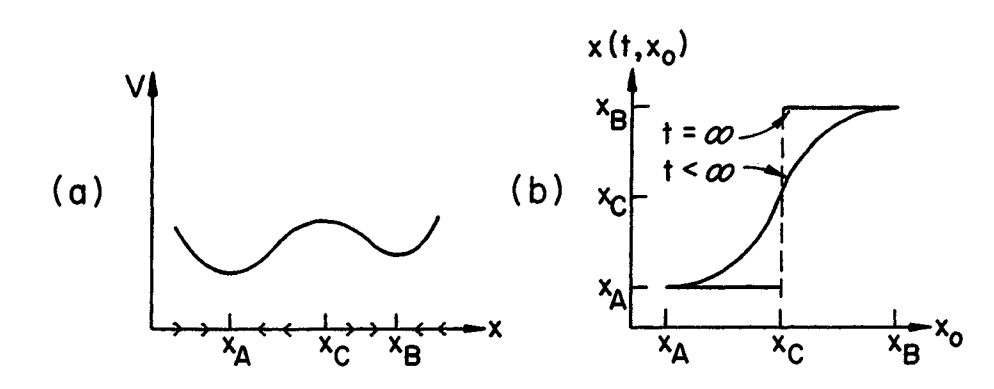
\includegraphics[width=13cm]{graphics/Bistable Evolution.png}
	\end{figure}
	For  $t=\infty$ it exhibits a discontinuity in the phase space diagram(or how you would call it). The set of initial conditions $\lbrace x_0 \rbrace$ which flow to a given fixed point is called the \textbf{basin of attraction} of that fixed point.
	
	The same principals apply when doing an infinite amount of RG-Transformations. Every Transformation is analytic but doing infinitely many can introduce singular behavior. With every RG-Transformation, the series $K_0^{(n)},K_1^{(n)} $ can be thought of as a point moving in coupling constant space (just like advancing time in our first example). A given system represented by its initial set of coupling constants traces out a trajectory in coupling constant space and the set of all those trajectories generates a \textbf{renormalization group flow}. The trajectories almost always become attracted to fixed points and we will see that scaling behavior is associated with the dynamics near a particular sort of fixed point and the nature of the fixed point gives information about the phase diagram of the system.
	
	\textbf{Fixed Points:} \\
	If we know the RG transformation $R_l[K]$, we define a fixed point $[K^*]$:
	\begin{equation}
		[K^*] =	R_l[K^*] \qquad \Rightarrow \quad \xi[K^*]  =	\xi[K^*] /	l
	\end{equation}
	Which implies that the Correlation length at the fixed point must be zero (trivial FP) or infinity (critical FP).
	\textbf{Reminder:} Temperature is nothing else than a coupling constant.
	
	Since $\xi[K] =	l^N \xi[K^{(N)}]$, all points in the basin of attraction of a critical fixed point have infinite correlation length. The basin of attraction is often called the critical manifold. The fact that all points on the critical manifold flow towards the same fixed point is the basic mechanism for universality. The critical fixed points describe the singular critical behavior, whereas the trivial fixed points describe the bulk phases of the system. Fixed points do not have to be isolated points, but can be lines and surfaces and this will be classified by their codimension ($c = d - d_{FP}$).
	\textbf{RG Flows near FP:} Consider a system near a fixed point $K_n =	K_n^* + \delta K_n$ and now perform an RG-Transformation, then:
	\begin{equation}
		K_n' = K_n^* + \delta K_n' \qquad \text{with} \qquad \delta K_m' =	\sum_m M_{nm} \delta K_m \quad \text{and} \quad M_{nm} =	\frac{\partial K_n'}{\partial K_m}\bigg|_{K=K^*}
	\end{equation}
	$M_{mn}$ is the linearised RG transformation in the vicinity of the fixed point $K^*$. We assume for now that $M$ is symmetric. We denote its eigenvalues and eigenvectors by $\Lambda_l^{(\sigma)}$ and $e_n^{(\sigma)}$ ($n$ is the component of the vector). Semi-group property of RG-Transformation implies:
	\begin{equation}
		M^{(l)}M^{(l')} =	M^{(ll')} \qquad \text{and thus} \qquad \Lambda_l^{(\sigma)}\Lambda_{l'}^{(\sigma)} =	\Lambda_{ll'}^{(\sigma)}
	\end{equation}
	The functional equation for the eigenvalues is solvable and yields:
	\begin{equation}
		\Lambda_{(l)}^{(\sigma)} =	l^{y_\sigma} \qquad \text{with $y_\sigma$ TBD}
	\end{equation}
	We now want to identify which coupling constant shrinks and which one grows, therefore we expand $\delta K$ in the eigendirections
	\begin{equation}
		\delta K =	\sum_\sigma 	a^{(\sigma)} e^{(\sigma)} \qquad \text{and} \qquad \delta K' =	M \delta K =	\sum_\sigma a^{(\sigma)} \Lambda^{(\sigma)} e^{(\sigma)}
	\end{equation}
	Those equations are very important since they tell us which components grow and shrink. We can distinguish three cases:
	
	\begin{enumerate}
		\item $|\Lambda^{(\sigma)}| >	1 \quad \Rightarrow \quad y^\sigma > 0 \quad \Rightarrow \quad a^{(\sigma)'}$ grows as l increases. (\textbf{relevant} EV)
		\item $|\Lambda^{(\sigma)}| <	1 \quad \Rightarrow \quad y^\sigma < 0 \quad \Rightarrow \quad a^{(\sigma)'}$ shrinks as l increases (\textbf{irrelevant EV})
		\item $|\Lambda^{(\sigma)}| =	1 \quad \Rightarrow \quad y^\sigma = 0 \quad \Rightarrow \quad a^{(\sigma)'}$ does not change (\textbf{marginal} EV)
	\end{enumerate}
	The flows away from ${K^*}$ i.e. in directions \textbf{out }of the critical manifold are associated with \textbf{relevant }eigenvalues. The \textbf{irrelevant} eigenvalues correspond to directions of flow \textbf{into} the fixed point. Remember that the terms relevant, ..., are always to be specified with respect to a particular fixed point.
	
	\textbf{Types of Fixed points:} The state of the system described by the fixed point it flows to represents the phase at the original point in the phase diagram, that's why it is useful to classify the fixed points. The type of fixed point depends on it's codimension and its correlation length. Lets call a fixed point with codimension $c=2$ and correlation lenght $\xi =	\infty$ \textbf{critical fixed point}. What happens to a system close to criticality? Trajectories of the system \textbf{on} the critical manifold remein on the manifold and flow towards the fixed point. Trajectories which start slightly off the critical manifold initially flow towards the critical fixed point, but ultimately are repelled from the critical manifold, because the critical fixed point has two unstable directions (two relevant directions).
	
	The fact that it is the \textbf{same eigenvalues} which drive \textbf{all} slightly off-critical systems away from the fixed point is the origin of universality. Thus, the initial values of the coupling constants do not determine the critical behavior. Only the flow behavior near the fixed point controls the critical behavior.
	
	The flow diagram for the Ising model with NNN:
	\begin{equation}
		\mathcal{H} =	K_1 \sum_{\langle ij \rangle} {S_i S_j} + K_2 \sum_{ij = NNN}^{} S_i S_j + h \sum_{i}^{} S_i
	\end{equation}
	is shown in the next figure. We can see here that the nearest neighbor and next nearest neighbor ising hamiltonians are in the same universality class (since they flow to the same FP? Or because they are both driven away from the Critical FP?). The High Temperature FP in the figure has codimension one (the relevant direction is out of the h=0 plane) and so attracts for high temps. The critical FP has two unstable directions, it doesn't even attract in the $h=0$ plane, here the flows direct to the high or low temperature FPs.
	\begin{figure}[htp]
		\centering
		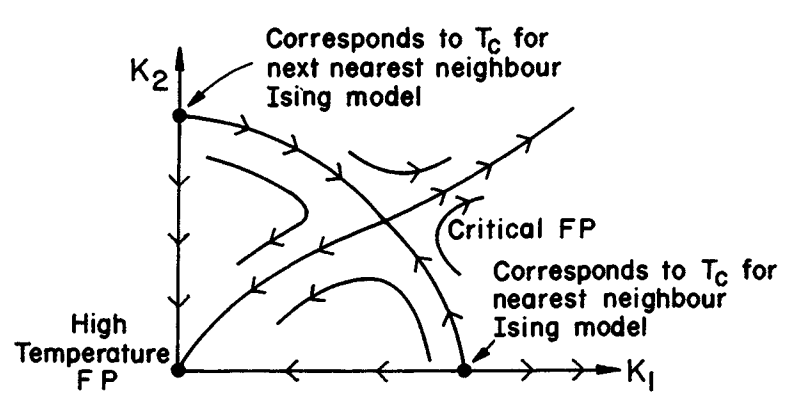
\includegraphics[width=12cm]{graphics/FP-Phase-Diagram.png}
	\end{figure}
	
	
	\textbf{Origin of Scaling:} \\
	Consider a System with only one coupling constant (the temperature $T$), so that we linearize in the vicinity of a fixed point and write
	\begin{equation}
		T' - T^* =	R_l(T) - R_l(T^*) \approx \Lambda_l(T - T^*) + O((T - T^*)^2)
	\end{equation}
	with $\Lambda_l = \frac{\partial R_l(T)}{\partial T}\big|_{T=T^*} =	l^{y_\epsilon}$. Using the reduced temperature the equation becomes
	\begin{equation}
		\epsilon' = \epsilon l^{y_\epsilon} \qquad \text{and after n RG-Iterations} \qquad \epsilon^{(n)} =	(l^{y_\epsilon})^n \epsilon
	\end{equation}
	For the correlation length we get
	\begin{equation}
		\xi(\epsilon) =	l^n \xi(\epsilon^{(n)}) =	l^n \xi(\epsilon l^{n y_\epsilon})
	\end{equation}
	We can choose $l$ arbitrary and our goal is to obtain a form for the correlation length where we can see the scaling with the temperature. Since we don't know the function $\xi(\epsilon')$, it would be smart to choose $l$ in a manner so that the argument of the function becomes constant. So we choose $l^n =	\left(\frac{b}{\epsilon}\right)^{1/y_\epsilon}$ so that we get
	\begin{equation}
		\xi(\epsilon) =	\left(\frac{\epsilon}{b}\right)^{-1/y_\epsilon} \xi(b) \qquad \text{Comparing with Definition for $\nu$} \quad \Rightarrow \quad \nu =	\frac{1}{y_\epsilon}
	\end{equation}
	\textbf{This is an important and central result}, since we know $y_\epsilon$ or at least can approximate it if we know $R_l$. We can make similar arguments for the free energy density and get
	\begin{equation}
		f(\epsilon) =	\left(\frac{\epsilon}{b}\right)^{d/y_\epsilon} f(b) \qquad \Rightarrow	 \qquad \frac{d}{y_\epsilon} =	2 - \alpha
	\end{equation}
	Which in combination with $\nu$ gives the \textbf{Josephson scaling law}
	\begin{equation}
		2 - \alpha =	\nu d
	\end{equation}
	With two coupling constants $\epsilon, h$, we get for the (singular part of the?) free energy density
	\begin{equation}
		f(t,h) =	l^{-nd} f(l^{ny_\epsilon \epsilon, l^{ny_h} h}) \quad \Rightarrow \quad f(t, h) =	t^{d/y_\epsilon} b^{-d} f(b, h / \epsilon^{y_h /	y_\epsilon}) \quad \text{with} \quad l^n =	b \epsilon^{-1/y_\epsilon}
	\end{equation}
	Which is the scaling form we got from the block spin argument that also recovers Josephson scaling law and
	\begin{equation}
		\Delta =	y_h/y_\epsilon
	\end{equation}
	
	\textbf{RG in differential form:} \\
	So, what we did was discrete RG, why discrete?
	For two RG-Transformations with $l$ and $s$ respectively, we already now that $[K]_{sl} =	R_s [K_l]$. Now choose $s =	1 + \varepsilon$ and the \textbf{differential RG transformation} is then obtained by
	\begin{equation}
		\frac{\text{d}[K_l]}{dl} =	\lim_{\varepsilon \rightarrow 0} \frac{[K]_{(1 + \varepsilon)l} - [K]_l}{\varepsilon l} \quad \text{with} \quad \lim_{\varepsilon \rightarrow 0} \frac{[K]_{(1 + \varepsilon)l} - [K]_l}{\varepsilon l} =	\frac{1}{l} \frac{\partial R_s[K_l]}{\partial s} \equiv \frac{1}{l} B [K_l]
	\end{equation}
	which defines the non-linear transformation $B[K_l]$. We can rewrite this(recursion relation?) with the time-like variable $\tau \equiv \ln (l) \Rightarrow \frac{\text{d}[K_\tau]}{\text{d} \tau} =	B[K_\tau]$. The fixed points are the solution of
	\begin{equation}
		B[K^*] =	0
	\end{equation}
	It seems to be possible to integrate the above defined non-linear ordinary differential equations out to any desired length scale where \textbf{perturbation theory} applies and then matching the solutions of the differential equations to the ones from perturbation theory.
	
	\textbf{RG Example:} \\
	Calculation for ising model on triangular lattice, just sketch the steps
	\begin{enumerate}
		\item	think of the transformation and figure out the length scale $l$ that it imposes
		\item Hard part:	Calculate the coarse grained Hamiltonian, you probably need to sum over the combined degrees of freedom to find the ansatz? Like $e^{\mathcal{H}'\lbrace S_I \rbrace} =	\sum_{\lbrace \sigma \rbrace} e^{\mathcal{H}(S_I, \sigma_I)}$. To find $\mathcal{H}'$ use approximations, pertubation theory, do some calculations... to bring it to the form of the original Hamiltonian (why is that legal?)
		\item Once you have $\mathcal{H}$ in the right form, read of the $K'$ and look at their dependence on $K$, this is your recursion relation.
		\item If you have identified your recursion relation, use it to calculate the eigenvalues of your linearized transformation in the means of $\Lambda_\epsilon =	\frac{\partial K'}{\partial K} \big|_{K^*}$ at the fixed points (which are also defined by the recursion relation). Combined with the length scale $l$ the eigenvalues give the critical exponents.
	\end{enumerate}
	Try to find such a transformation for your system?
	
	\textbf{Crossover Phenomena:} \\
	Crossover phenomena are phenomena associated with the failure of a system to attain its asymptotic scaling regime. Besides other things, interactions that break the symmetry might generate relevant directions at fixed points which are not associated with the external variables such as temperature. For me this would be the double Well potential that breaks the $O(2)$ - Symmetry of my pointers (Or the translation symmetry for $z$) (or at least it would be a bit like that? It is not weak but yeah).
	
	An example for this would be the Heisenberg-Model with a single ion anisotropy
	\begin{equation}
		\mathcal{H} = K \sum_{\langle ij \rangle}^{} S_i S_j + g \sum_{i} (S_i^z)^2
	\end{equation}
	Which looks a bit like my quadratic interaction with a harmonic trap in one direction, which could reproduce my system (at least with anisotropic interaction). At high temperatures we still expect a paramagnetic phase, but at low temperatures the spins align and if $g > 0$ the spins can lower the energy $H =	-k_B T \mathcal{H}$ by aligning along th z axis and at low enough temperatures
	\begin{equation}
		\langle S_i^z \rangle =	\pm 1
	\end{equation}
	Which is a stat characteristic of the low temperature behavior of the Ising model. A consequence of these considerations is that, for large g, the phase transition from the paramagnetic phase as T is reduced will be in the Ising universality class (for $g>0$, for $g < 0$ it will be in the XY universality class.). For non-zero values of $g$, $g$ will grow under renormalization and will carry the system towards the Ising fixed point and around this fixed point, the scaling phenomena will be different from those of the Heisenberg fixed point.
	
	To describe this crossover phenomenon, we use two relevant scaling fields near the Heisenberg fixed point. One is $\epsilon$, the other is $g$ and the singular part of the free energy density will transform as:
	\begin{equation}
		f_s(\epsilon, g) =	l^{-d} f_s(tl^{y_\epsilon}, gl^{y_g}) =	|\epsilon|^{2 - \alpha} F_{\pm}(g|\epsilon|^{-\phi})
	\end{equation}
	with the \textbf{crossover exponent} $\phi = y_g / y_t > 0 \quad (\text{since}~ y_g > 0 \quad (\text{since g grows?}))$. This implies that we expect Ising behavior when $|g| |\epsilon|^{-\phi} \gg 1$.
	
	\textbf{Corrections to Scaling:} \\
	We already heard in the section mean field theory that it is difficult to access the asymptotical critical regime and we therefore need to consider corrections to scaling. Consider the susceptibility:
	\begin{equation}
		\chi_T(\epsilon, h) = |\epsilon|^{-\gamma} F_\chi^{\pm} \left(\frac{h}{\epsilon^\Delta} , \tilde{K}_3 \epsilon^{-y_3 / y_t}, ... \right)
	\end{equation}
	with $\tilde{K}_3$ being an irrelevant scaling field and $y_3 < 0$. The scaling function should be analytic so we expand it for small values of its arguments:
	\begin{equation}
		\chi_T(\epsilon, 0) =	|\epsilon|^{-\gamma} \left(A_\pm + B_\pm \tilde{K}_3 |\epsilon|^{-y_3 /	y_\epsilon} + ... \right)
	\end{equation}
	The leading behavior at $\epsilon \rightarrow 0$ is $|\epsilon|^{-\gamma}$, but there is a first correction of order $|t|^{-y_3 / y_\epsilon}$. Depending on the cases $|y_3| / y_\epsilon \lessgtr 1$ the correction becomes smaller as we approach the critical point, or grows and is therefore not even negligible for small $\epsilon$. Such a correction is called a \textbf{confluent singularity}.
	
	For the Ising universality class (which dimension?), the leading correction term due to irrelevant variable is
	\begin{equation}
		y_3 / y_t \approx 0.5
	\end{equation}
	(How do we know what $y_3$ is, doesn't this depend on the specific hamilton? I think it is the greatest irrelevant variable, but what if we don't even have three coupling constants?) \textbf{This correction is observed in numerical calculations and must be taken into account when attempting to extract critical exponents from data}.
	
	\textbf{Finite Size scaling}\\
	Again: strictly speaking there are no phase transitions in a finite system at non-zero temperature and in real life or (especially) numerical calculations we always work with finite systems. How does this effect the RG and what can we nevertheless learn about the phase transition? Consider a system of size $V = L^d$. $L$ transforms after the RG-transformation like $L' = L/l$. Therefore the singular part of the free energy density, written in dependency of the system size, scales like
	\begin{equation}
		f_s([K], L^{-1}) =	l^{-d} f_s([K'], l L^{-1})
	\end{equation}
	Close to a fixed point of the RG, we can write this in terms of eigenvectors and eigenvalues
	\begin{equation}
		f_s(t, h, \tilde{K}_3, ..., L^{-1}) =	l^{-d} f_s(t l^{y_t}, h l^{y_h}, \tilde{K}_r l^{y_3}, ..., l L^{-1})
	\end{equation}
	We can see that $L^{-1}$ behaves like a relevant eigenvector with eigenvalue
	\begin{equation}
		\Lambda_L =	l \qquad \Rightarrow \qquad y_L = 1
	\end{equation}
	$L^{-1}$ is a relevant parameter that has to be tuned to $L^{-1} = 0$ for the phase transition to happen, as well as $\epsilon = 0$. So we see that in this context $\epsilon$ is the critical temperature in the thermodynamic limit.
	
	So for finite L, crossover effects become important. Consider the singular part of the free energy density at $h=0$:
	\begin{align}
		f_s(\epsilon, L^{-1}) &= |\epsilon|^{2 - \alpha} F_f^\pm(L^{-1} |\epsilon|^{y_L / y_\epsilon}) \\
		&= |\epsilon|^{2 - \alpha} F_f^\pm(L^{-1} |\epsilon|^{-1 / y_\epsilon}) \\
		&=	|\epsilon|^{2 - \alpha} F_f^\pm(\xi_\infty L^{-1}) \quad \text{with bulk corr length of  $\infty$-system} \quad \xi_\infty(\epsilon)
	\end{align}
	The true critical behavior happens if $L^{-1} = 0$, so in the limit $x \rightarrow 0$ of $F_f^\pm(x)$, meaning, when $L^{-1}\epsilon^{-\nu} \ll 1$, or equivalently $L \gg \xi_\infty(\epsilon)$, then the correlation length is not affected by the boundaries of the system and the thermodynamic properties are those of the infinite system.
	
	The scaling of the specific heat has a similar form like above:
	\begin{align}
		c(\epsilon, L^{-1}) &=	|\epsilon|^{-\alpha} F_f^\pm(L^{-1} |\epsilon|^{-\nu}) \\
		&= |\epsilon|^{-\alpha} (L^{-1}t^{-\nu})^{-\alpha/\nu} D^\pm (\epsilon L^{1/\nu}) \\
		&= L^{\alpha/ \nu} D^\pm (\epsilon L^{1/\nu})
	\end{align}
	with the new defined scaling function $D(x)$ (with a maximum at $x = x_0$?). The specific heat peak therefore occurs at a reduced temperature shifted from that in the infinite system by an amount
	\begin{equation}
		\epsilon_L = x_0 /	L^{1/\nu} \propto L^{-1/\nu}
	\end{equation}
	And the maximum height is
	\begin{equation}
		c(\epsilon_L, L^{-1}) = L^{\alpha/\nu} D(x_0) \alpha L^{\alpha/\nu}
	\end{equation}
	The next figure shows a sketch for the specific heat capacity for infinite and finite systems.
	\begin{figure}[htp]
		\centering
		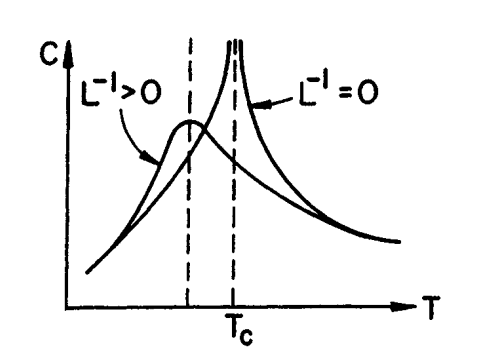
\includegraphics[width=10cm]{graphics/heat-finite-system.png}
	\end{figure}
	We can exploit these phenomena in practice to obtain estimate of the true critical behavior. Consider the finite size scaling of the correlation length itself
	\begin{align}
		\xi(\epsilon, L^{-1}) &=	l \xi(\epsilon l^{y_t}, l L^{-1}) \\
		&=\varepsilon^{-\nu} F_\xi (L^{-1} \varepsilon^{-\nu}) \\
		&= \varepsilon^{-\nu}(L \varepsilon^\nu) \bar{F}(L\epsilon^\nu) \\
		&=L \bar{F}(L\epsilon^\nu)
	\end{align}
	With again a new scaling function $\bar{F}(x)$, which must have the following limiting behavior: For $L \rightarrow \infty$ at fixed $\epsilon \ll 1$, we expect $\xi(\epsilon, 0) \sim \epsilon^{-\nu}$, thus $\bar{F}(x) \rightarrow x^{-1} $ as $x \rightarrow \infty$. For L finite and $t \rightarrow 0$, $\bar{F}(x)$ tends towards a constant (since the correlation length cant get greater than L? $\xi \sim L$). At finite L we can expand about $\epsilon =0$ \cite{pelissetto2002critical} \cite{goldenfeld2018lectures}:
	\begin{equation}
		\frac{L}{\xi(\epsilon, L^{-1})} =	A + B \epsilon L^{1/\nu} + O(\epsilon^2)
	\end{equation}
	This is a very important equation, since if we plot $L/\xi$ versus the coupling constant $K$ (in this case $\epsilon$), for different values of L, all the curves will pass through the same point when $K =	K^*$, thus we can determine $K^*$ (or in this case, the critical temperature). We can also compute the the critical exponents, using the fact that
	\begin{equation}
		\frac{\partial}{\partial K} \left(\frac{L}{\xi(\epsilon, L^{-1})}\right) = B L^{1/\nu} \quad \text{or in practice via} \quad \ln \frac{\partial}{\partial K}\left(\frac{L}{\xi}\right) =	\ln B + \frac{1}{\nu} \ln L
	\end{equation}
	
	I am not sure if those equations already use the corrections to scaling or if they are totally independent from them. The next figure shows a sketch of th finite size scaling of the correlation length:
	
	\begin{figure}[htp]
		\centering
		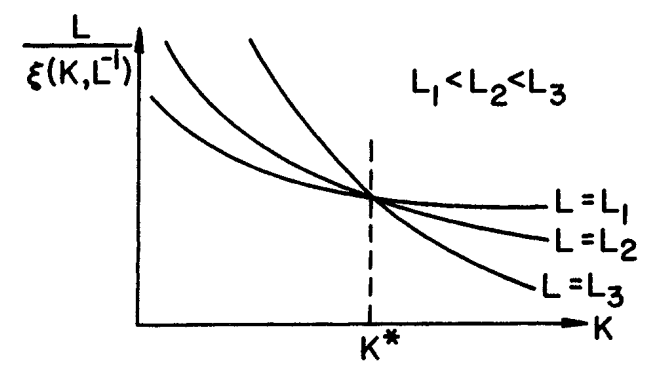
\includegraphics[width=12cm]{graphics/corr-ffs.png}
	\end{figure}
	
	The equations above neglect corrections to scaling. And how to consider them will be explained in the following. We consider some so called ''phenomenological couplings'' like the binder cumulant $U_L$:
	\begin{equation}
		U_L =	\frac{\langle m_L^4 \rangle}{\langle m_L^2 \rangle^2}
	\end{equation}
	It is important that we are aware that $m_L$ is the magnetization of a system of size $L$, but to get correct results, we need to simulate a large system and look at the magnetization of subsystems of size $L$. $m_L$ is therefore basically the coarse grained local magnetization.
	
	Another phenomenological coupling is $\xi_{2nd}/L$, with $\xi_{2nd}$ being the ''\textbf{second moment correlation length}'' which seems to have better properties for numerical extraction and converges fast to the actual correlation length $\xi_{exp} = \xi$
	
	We will denote the phenomenological couplings with $R$. Their finite size scaling can be shown \cite{hasenbusch2008critical} to follow
	\begin{equation}
		R(\varepsilon, L) =	R^* + r' \varepsilon L^{y_\varepsilon} + ... + c_\omega L^{-\omega}
	\end{equation}
	close to the critical point. $\omega =	- y_\omega$ is the RG dimension of the leading irrelevant scaling field (irrelevant coupling constant). At the critical point, all systems assume the value $R^*$ and therefore intersect. We can extract the critical temperature this way. A plot for my system is shown in the next figure.
	
	\begin{figure}
		\centering
		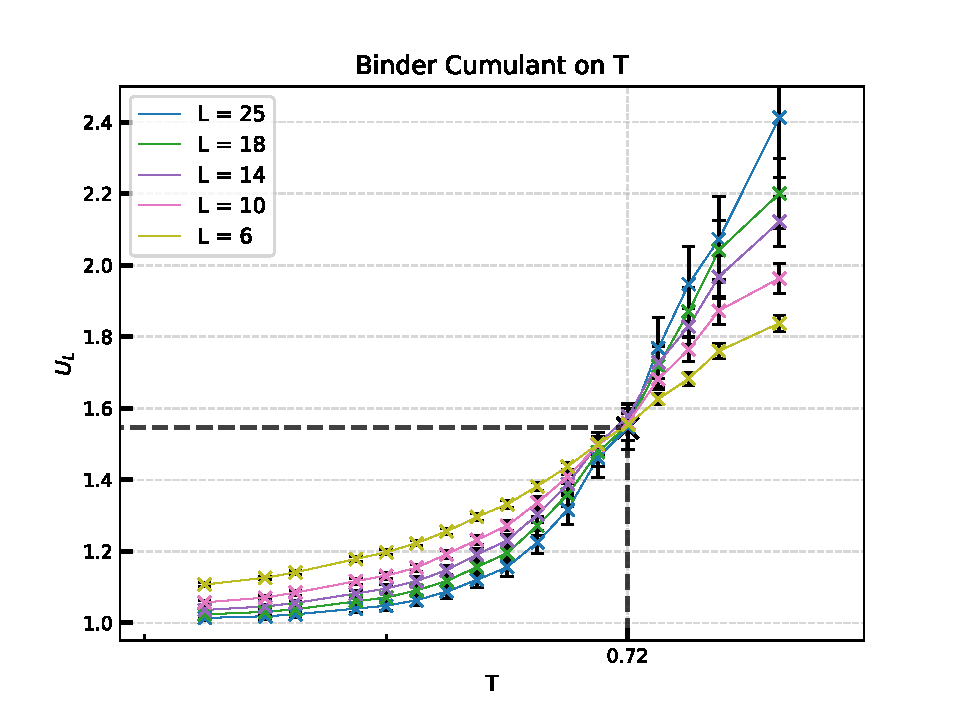
\includegraphics[width=13cm]{graphics/binder-cum.pdf}
	\end{figure}
	
	By deriving the finite size scaling law for the reduced temperature (neglecting the corrections) we obtain (in the region where this form is valid, so for $\varepsilon \approx 0 $)
	
	\begin{equation}
		\ln \frac{d R}{d \varepsilon} \Big |_{\varepsilon =	0} =	\ln \left(r' L^{y_\varepsilon} \right) =	\ln(r') + y_\varepsilon 	\ln L =	\ln(r') + \frac{1}{\nu}	\ln L
	\end{equation}
	So we can derive the Binder cumulant at the critical temperature (for the reduced temperature) for the different sizes and do a linear fit to extract the critical exponent. Like shown in the next figure.
	\begin{figure}
		\centering
		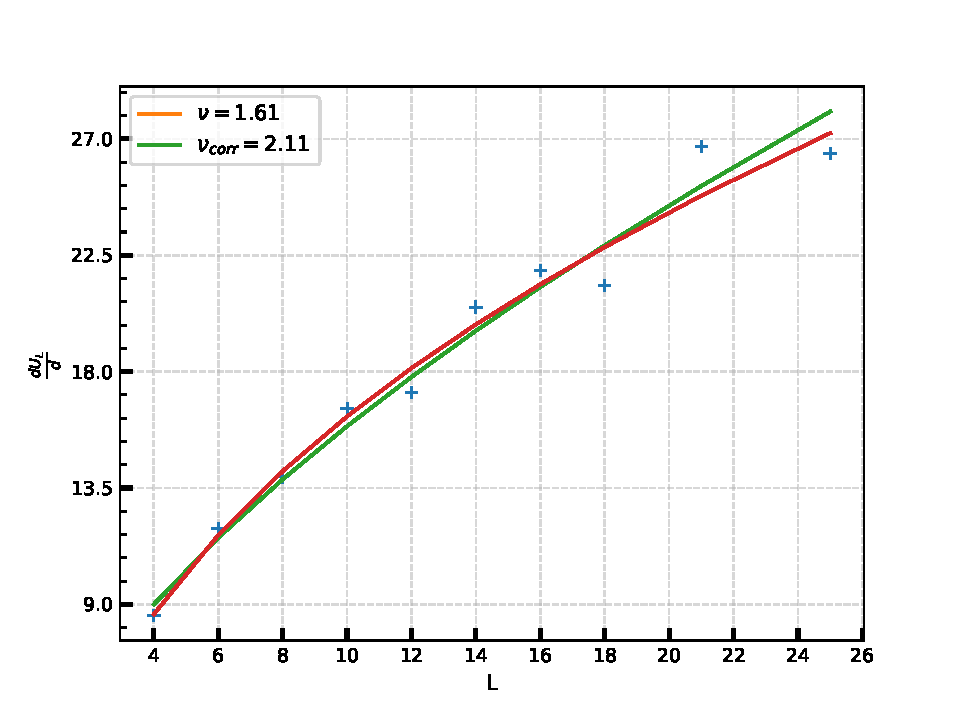
\includegraphics[width=12cm]{graphics/critical_exponent.pdf}
	\end{figure}
	
	The critical Exponents for relevant Models are
	\begin{center}
		\begin{tabular}{ c c c c}
			Model & $\nu$ & $\omega$ &  $\mu$ \\
			\hline
			Ising 2D & 1 & 2 & 2.14\\
			My Model & 1.2 - 2 & ? & 2 - 3
		\end{tabular}
	\end{center}
	The initial thought was that we should be in Ising universality class they share \textbf{$\boldsymbol{\mathbb{Z}_2}$-Symmetry}, \textbf{short-range interactions} (we are using coulomb which is actually long range but since we only consider NN it should still be short range?) and \textbf{dimensionality $\mathbf{d=2}$}.
	
	\subsubsection{Nonequilibrium Relaxation method}
	Another method for the extraction of critical exponents and estimation of the transition temperature. The idea is that we do not need to let the model relax to equilibrium but deduce the critical exponents from the way that the system approaches equilibrium.
	
	\textbf{Estimation of $T_c$:}
	
	We record the order parameter, in our case $m(t)$, called the \textbf{NER function}. The asymptotic relaxation of $m(t)$ for large $t$ in the different phases is summarized as
	\begin{equation}
		m(t) \sim \begin{cases}
			e^{-t /	\tau} \quad (T > T_c) \\
			t^{-\lambda_m} \quad (T =	T_c) \\
			m_{eq} \quad (T < T_c)
		\end{cases}
	\end{equation}
	With corrections, at the critical point
	\begin{equation}
		m(t) =	A t^{-\lambda_m} (1 + B / t^\omega)
	\end{equation}
	\begin{figure}[htp]
		\centering
		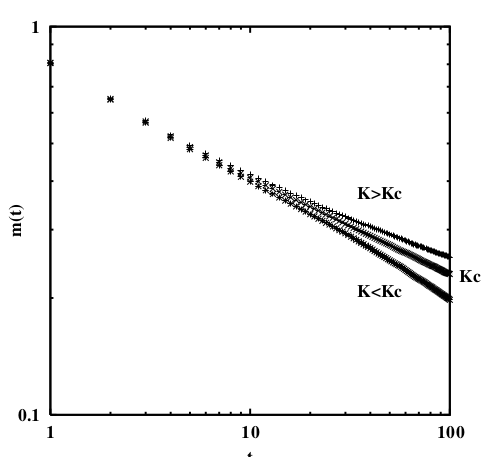
\includegraphics[width=10cm]{graphics/NER-m.png}
		\caption{Just a caption}
		\label{NER-m}
	\end{figure}
	
	is valid. Only at the critical temperature the $m(t)$-curve will be a line in a log-log-plot (see \autoref{NER-m}). So we can roughly estimate the critical temperature by looking at which temperatures the curves start to bend up- or downwards.
	
	It is usually easier to see if we fit for $\lambda_m$ and see for which temperature it stays constant in dependence of $t$. We practically do this by fitting the line equation
	\begin{equation}
		y =	\ln \left(m(t)\right) =	\ln \left(1 + B /	t^\omega \right) + \ln A - \lambda_m \ln t
	\end{equation}
	to our data in certain intervals $\left[t, t + \Delta t\right]$. For large $t$, the function $\lambda_m(t)$ should become constant (\autoref{NER-lambda_m}).
	\begin{figure}[htp]
		\centering
		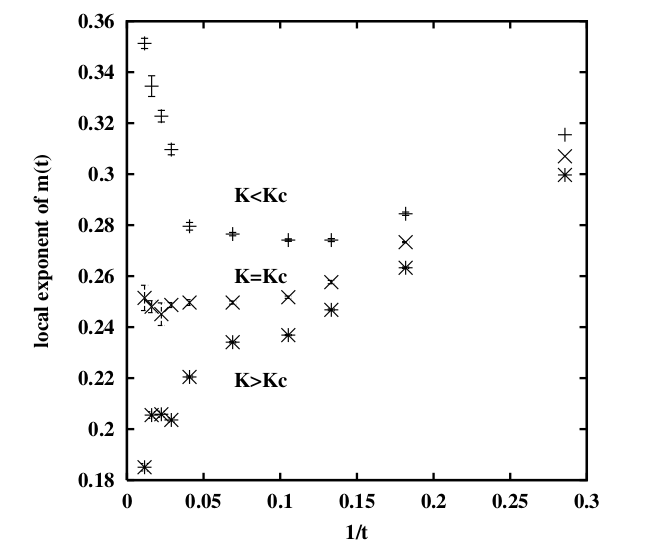
\includegraphics[width=10cm]{graphics/NER-lambda_m.png}
		\caption{Just a caption}
		\label{NER-lambda_m}
	\end{figure}
	
	\textbf{Estimation of $z$ and $\nu$:}
	
	From renormalization group considerations \cite{ozeki2007nonequilibrium} we can identify the relation
	\begin{equation}
		\lambda_m =	\frac{\beta}{z \nu}
	\end{equation}
	But since we don't know any of those exponents for our model beforehand, we need some more information. We get that from the \textbf{NER	fluctuation functions}, which are basically the susceptibility $\chi$, the specific heat $C$ and $\frac{\partial m(t)}{\partial T}$ over time $t$. We write their definition in dimensionless form:
	\begin{equation}
		(\chi) \quad f_{mm}(t) =	n \left[\frac{\left\langle m^2\right \rangle_t}{\left\langle m\right \rangle_t^2} - 1 \right] \quad \text{and} \quad \left(\frac{\partial m}{\partial T}\right) \quad f_{me}(t) =	n \left[\frac{\left\langle me\right \rangle_t}{\left\langle m\right \rangle_t  \left\langle e \right \rangle_t} - 1 \right]
	\end{equation}
	where $ \left\langle e \right \rangle$ is the average energy per site. From the critical power law divergence of $\chi$ and $\frac{\partial m(t)}{\partial T}$ \cite{sadiq1984dynamics}, we make the scaling ansatz
	\begin{equation}
		f_{mm} \sim t^{\lambda_{mm}} \qquad \text{and} \qquad f_{me} \sim t^{\lambda_{me}}
	\end{equation}
	and identify
	\begin{equation}
		\lambda_{mm} =	\frac{d}{z} \qquad \text{and} \qquad \lambda_{me} =	\frac{1}{z \nu}
	\end{equation}
	
	The \textbf{local exponents} are defined as
	\begin{equation}
		\lambda_{mm}(t) =	\frac{d\ln f_{mm} (t)}{d\ln t} \qquad \text{and} \qquad \lambda_{me}(t) =	\frac{d\ln f_{me} (t)}{d\ln t}
	\end{equation}
	and are supposed to converge to their time independent correspondents for $t \rightarrow \infty$. In practice we plot the local exponents vs $1/t^\Omega$ and extrapolate to $ 1 /	t^\Omega =	0$. The value of $\Omega$ depends on the system and the exponent we are considering and is expected to be a result of corrections from irrelevant scaling fields \cite{yao2001appc}.
	One can also define the local exponents
	\begin{equation}
		z(t) = \frac{d}{\lambda_{mm} (t)} \qquad \text{and} \qquad \nu(t) =	\frac{\lambda_{mm}(t)}{d \cdot \lambda_{me}(t)}
	\end{equation}
	The extrapolation to $t \rightarrow \infty$ is shown for $\nu (t)$ in \autoref{NER-nu}.
	
	\begin{figure}[htp]
		\centering
		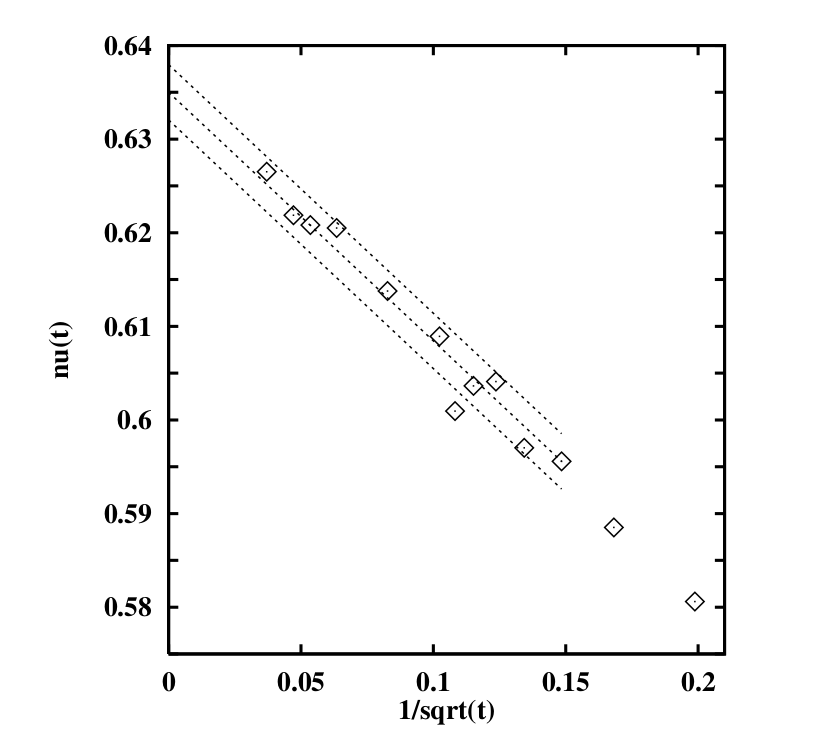
\includegraphics[width=10cm]{graphics/NER-nu.png}
		\caption{just a caption}
		\label{NER-nu}
	\end{figure}
	For me, this is obviously not working again.
	\subsection{Kibble-Zurek-Mechanism}
	\label{KZM}
	\subsubsection{Phenomenological Approach}
	So what happens really phenomenologically is that the correlation lenght as well as the relaxation time diverge at the phase transition, at least in the thermodynamic limit. A diverging correlation lenght would actually mean, that every lattice site in the system is correlated with one another, but causality and the diverging of the relaxation time forbid this. Two lattice sites in two points of spacetime can only be correlated, if their separation is less than the distance light can travel in their time difference. So two lattice sites far apart from each other cannot be correlated during/after the phase transition, if the phase transition was faster than light/sound would have needed to travel between the two sites. In other words: the relaxation time diverges because the equilibrium correlation length diverges and it would take an infinite amount of time to correlate two infinitly far apart lattice sites since the speed of sound is finite.
	
	That being said, it is obvious that two lattice sites far apart can take on different values since they are totally uncorrelated. And if thats the case, there has to be a domain wall between the two sites. The Problem of the KZM is to describe the scaling of the density of those domain walls depending on how fast the phase transition took place. We can already very intuitively say that faster phase transitions will result in higher densities, since the system won't have much time to equilibriate.
	
	\subsubsection{Mathematical basics}
	From RG-Theory, we know the scaling of the correlation length and the relaxation time:
	\begin{equation}
		\xi \propto \epsilon^{-\nu} \qquad \tau \propto \epsilon^{-\mu}
	\end{equation}
	And I think we also know the connection between the critical exponents \cite{goldenfeld2018lectures}
	\begin{equation}
		\nu z = \mu
	\end{equation}
	
	We introduce proportionality constants with $\xi =	\xi_0 $ at $\epsilon = 1$ and analogous for $\tau$:
	\begin{equation}
		\xi =	\frac{\xi_0}{|\epsilon|^\nu} \qquad \tau =	\frac{\tau_0}{|\epsilon|^\mu}
	\end{equation}
	Another way to look at this would be to say: The equilibration time to equilibrate to the correlation length $\xi$ scales with $\xi$ as
	\begin{equation}
		\tau \propto \xi^z \qquad \Rightarrow \qquad \tau \propto \varepsilon^{-z\nu} \qquad \Rightarrow \mu =	z \nu
	\end{equation}
	The question would be to find out those equilibrium values for my system. Can we calculate this somehow? It will surely not work if we try to calculate it at different times in the phase transition and fit it like they did in the Zurek paper. My Correlation lenght wont diverge at $\epsilon =	0$. And especially not for my finite system.
	
	We can also 'define' another understanding of the correlation length. The correlation lenght ist the distance over which the order parameter returns back to its equilibrium value, when perturbed, meaning that the \textbf{correlation function} of perturbations $\delta \phi(x,t) =	\phi(x,t) - \left\langle \phi \right\rangle $ behaves as
	\begin{equation}
		\left\langle \delta \phi(x,t), \delta \phi(x + r,t) \right\rangle \propto e^{- |r| / \xi}~.
	\end{equation}
	The question is what the proportionality constant is, otherwise i cannot get quantitative values.
	
	Usually in the KZM we assume a linear quench, so that the temperature changes linearly with time:
	\begin{equation}
		\epsilon =	\frac{t}{\tau_Q}
	\end{equation}
	Here, $\tau_Q$ is the Quench time scale. If it is large, the Quench is slow.
	
	For arbitrary $\tau_Q$, there will come a time, where the derivative of $\xi$ becomes larger than the speed of sound. Meaning, that the equilibrium correlation length grows faster, than correlations could possibly propagate. So the \textbf{actual} correlation length will grow with the speed of sound, but it won't be able to keep up with the equilibrium correlation length. This can also be called \textbf{critical slowing down}. This will approximately happen when the relaxation time equals the time that remains to the phase transition. We could say, at this point, i would have exactly enough time to equilibriate to my equilibrium correlation length in $\hat{t}$ if my system didn't change anymore. But know i reduce the temperature further, so i won't have a chance to equilibriate. So when
	\begin{equation}
		\tau(\hat{t}) =	\hat{t} \qquad \text{and} \qquad \tau(\hat{t}) =	\tau(\hat{\varepsilon}) =	\tau_0 |\hat{\varepsilon}|^{-\mu} =	\tau_0 \Big |\frac{\hat{t}}{\tau_Q} \Big |^{-\mu}
	\end{equation}
	the equilibrium correlation length will start to outgrow the actual correlation length. The correlation length won't be able to converge. Instead, it will only approximately reach the value that it has at the freeze out time $\hat{t}$:
	\begin{equation}
		\hat{\xi} \approx \frac{\xi_0}{|\hat{\epsilon}|} =	\xi_0 \left( \frac{\tau_Q}{\tau_0}\right) ^{\nu/(1+\mu)} \qquad \text{with} \qquad \hat{\epsilon} =	\epsilon(\hat{t}) =	\frac{\hat{t}}{\tau_Q}
	\end{equation}
	It would surely be good to know those exponents for my system? Do I have to categorize it in an universality class for that? Then we could directly estimate the scaling.
	
	In practice, one would surely fit the logarithm of this relation:
	\begin{equation}
		\log \hat{\xi} =	\log \xi_0 - \frac{\nu}{1 + \mu} \log \tau_0 + \frac{\nu}{1 + \mu} \log \ \tau_Q
	\end{equation}
	The two former terms are just contants and can be absorbed in one. Getting the exponents results in extracting the slope of this equation.
	More accurately, $\xi$ will probably reach a value like
	\begin{equation}
		\hat{\xi} =	\xi(\hat{t}) + v_s \cdot \hat{t}
	\end{equation}
	With the speed of sound $v_s$. But the second term is probably not so important for scaling. Anyways, regions that are more distant than $\hat{\xi}$ will be 'forced' to select the new vacuum (their equilibrium) independently.
	
	[Source of this picture with the correlation length growing linearly?]
	corr
	For the defect density this means that it will be in leading order \textbf{given by }$\hat{\xi}$. But we have to \textbf{take into account that the choices of some domains might be similar anyway}.
	
	In the paper they do some more estimates for overdamped evolution and rewrite Eq. 9 with the dampening coefficient to estimate $\mu = 1$. Then they adopt $\nu =	1/2$ from Landau-Ginzburg (Isn't that a mean field prediction?) and find that
	\begin{equation}
		\hat{\xi} \propto \tau_Q^{\alpha} \qquad \text{with} \qquad \alpha = 1/4
	\end{equation}
	The numerical simulation with Langevin equation yields $\alpha = 0.28 \pm 0.02$. The number/density of kinks
	\begin{equation}
		n  \approx \frac{1}{f \cdot \hat{\xi}}
	\end{equation}
	Is satisfied for $f=8$. Problem for me: I cannot just count zeros like they did in a paper and with the raw eye it is also not possible. But i don't think i actually need this f.
	
	The critical exponent of the 2D Ising universality class is approximately $z \approx 2.15$ \cite{adzhemyan2022dynamic} \cite{dammann1993dynamical}.
	
	\subsection{Correlation Function and Correlation Length}
	The Definition of the Corr
	elation Function in 2D is
	\begin{equation}
		C(q, s) = \langle \sigma_{i,j} \sigma_{i +q ,j +s} \rangle = \lim\limits_{m \rightarrow \infty } \lim\limits_{ n \rightarrow \infty}	\frac{1}{Z(\beta)} \sum_{\lbrace\sigma\rbrace} \sigma_{i,j} \sigma_{i +q ,j +s} e^{- \beta \epsilon(\lbrace \sigma \rbrace)}
	\end{equation}
	If every state is equally probable, we can simplify the explicit expression as
	\begin{equation}
		\langle \sigma_{i,j} \sigma_{i +q ,j +s} \rangle = 	\frac{1}{m \cdot n} \sum_{i, j} \sigma_{i,j} \sigma_{i +q ,j +s}
	\end{equation}
	Actually, $\langle \cdot \rangle$ denotes the thermic average, so the average over multiple realizations of the system. I don't know the mathematically rigorous explanation, but we just average over the lattice sites of one system and over multiple system of the ensemble simultaneously.
	For the 2D anisotropic Ising Model, we can write down the Correlation Function in the limit for large distances as:
	\begin{equation}
		C(q, s) = \langle \sigma_{i,j} \sigma_{i +q ,j +s} \rangle \sim \frac{f_\gtrless(\theta)}{r^{\vartheta_\gtrless}} 	e^{-r /	\xi_\gtrless(\theta)} \qquad \text{with} \qquad r =	\sqrt{q^2 + s^2}
	\end{equation}
	\begin{figure}
		\centering
		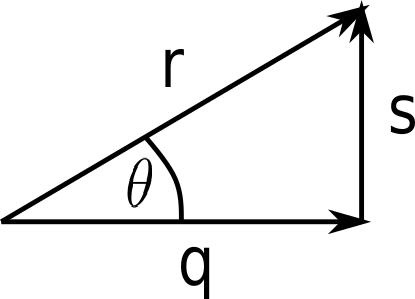
\includegraphics[width=5cm]{graphics/corr-func-angle.png}
	\end{figure}
	With known Functions $f_\gtrless(\theta)$ and $\xi_\gtrless(\theta)$ depending on the angle of the correlation vector and the Temperature $ T \gtrless T_c$. The exponent $\vartheta_\gtrless$ is for the Ising model $\vartheta_< =	2$ and $\vartheta_> = 1/2$.
	To find out the complete function of the correlation length would be pretty difficult, since we would need to calculate for every distance and every angle. For now, we are only interested in
	\begin{equation}
		\xi_x =	\xi(\theta = 0) \quad \Rightarrow \quad s =	0 \qquad \text{and} \qquad \xi_y = \xi(\theta = \pi /	2) \quad \Rightarrow \quad q = 0
	\end{equation}
	so we can write
	\begin{align}
		&C(q, 0) =	C_x(q) = \langle \sigma_{i,j} \sigma_{i +q ,j} \rangle \sim \frac{f_x}{q^{\vartheta_\gtrless}} 	e^{-q /	\xi_x} \qquad \\
		&C(0, s) =	C_y(s) =	\langle \sigma_{i,j} \sigma_{i ,j + s} \rangle \sim \frac{f_y}{s^{\vartheta_\gtrless}} 	e^{-s /	\xi_y} \qquad
	\end{align}
	We now look at the Fourier Transform of $C(q, 0)$ and $C(0, s)$ and for simplicity only do the calculation for $C(q, 0)$. To do that, we first look at the 2D Fourier Transform of $C(q, s)$ assuming we are on a lattice with $n$ columns and $m$ rows:
	\begin{equation}
		S(k, l) =	\sum_{q = 0}^{n-1} \sum_{s = 0}^{m-1} C(q, s) e^{-2\pi \mathrm{i} \left(\frac{qk}{n} + \frac{sl}{m}\right)}
	\end{equation}
	And now set $s=0$. (Or would we just do the fourier transform of $C_x$, which would yield in another normalization factor):
	\begin{equation}
		S(k, l) = S_x(k) =	\sum_{q = 0}^{n-1} \sum_{s = 0}^{m-1} C_x(q) e^{-2\pi \mathrm{i} \left(\frac{qk}{n}\right)} = m \cdot \sum_{q = 0}^{n-1} C_x(q) e^{-2\pi \mathrm{i} \left(\frac{qk}{n}\right)}
	\end{equation}
	We now insert the explicit form of the correlation function from above, which yiels
	\begin{equation}
		S_x(k) = \frac{1}{n} \cdot \sum_{q = 0}^{n-1} \left(\sum_{i = 0}^{n-1} \sum_{j =	0}^{m - 1} \sigma_{i,j} \sigma_{i +q ,j}\right) e^{-2\pi \mathrm{i} \left(\frac{qk}{n}\right)}
	\end{equation}
	We now make an index shift $p =	i + q$ and rearange the sums (indexes are a bit wobbly here but i am sure it is right anyway):
	\begin{equation}
		S_x(k) = \frac{1}{n} \cdot \sum_{j = 0}^{m-1} \left(\sum_{i = 0}^{n-1} \sum_{p = 0}^{n - 1} \sigma_{i,j} \sigma_{p ,j} e^{-2\pi \mathrm{i} \left(\frac{(p-i)k}{n}\right)} \right) =	 \frac{1}{n} \cdot \sum_{j = 0}^{m-1} \left(\sum_{i = 0}^{n-1} \ \sigma_{i,j} e^{2\pi \mathrm{i}\frac{ik}{n}} \right) \left( \sum_{p = 0}^{n - 1}\sigma_{p ,j} e^{-2\pi \mathrm{i} \frac{pk}{n}} \right)
	\end{equation}
	Now the last to sums look like the 1D Fourier Transform of the \textbf{row} $j$, which will now be denoted as $\tilde{\sigma}_j^x(k)$. With that we get
	\begin{equation}
		S_x(k) = \frac{1}{n} \cdot \sum_{j = 0}^{m-1} \left(\tilde{\sigma}_j^x(k)\right)^* \tilde{\sigma}_j^x(k)  =	\frac{1}{n} \cdot \sum_{j = 0}^{m-1} |\tilde{\sigma}_j^x(k)|^2 =	\frac{m}{n} \left\langle |\tilde{\sigma}^x(k)|^2 \right\rangle
	\end{equation}
	What we have achieved now is that the structure function in x direction is proportional to the  squared absolute value of the 1D Fourier Transformation of a \textbf{single row}, averaged over all rows. Which I think is \textbf{NOT} the same as: $S_x(k) \sim \left\langle |\tilde{\sigma}(k)|^2 \right\rangle$ the average of the ''normal'' 2D Fourier Trafo of the lattice.
	
	How does this help us to get the correlation length? Since we know $S_x(k)$ is the Fourier Transformation of $C_x(q)$ and we know the asymptotic behaviour of $C_x(q)$, which is approximately
	\begin{equation}
		C_x(q) \sim e^{-q /	\xi_x} \qquad \Rightarrow \qquad \Re\left(\tilde{C}_x(k)\right) = \Re \left(S_x(k) \right) \sim \frac{2 \xi_x}{1 + 4 \pi^2 k^2 \xi_x^2}
	\end{equation}
	we can extract the Correlation Length by calculating the averaged 1D Fourier Trafo of the Lattice, fitting a Lorentzian peak to it and extracting the width of the peak.
	
	\subsubsection{Inverse considerations}
	It is easier to find a relation to fit the correlation length by going the inverse way. We write down the 2D DFT of the order parameter:
	\begin{equation}
		\tilde{\sigma}_{kl} =	\sum_{i =	0,j = 0}^{n-1} \sigma_{ij} e^{-2 \pi i \frac{ik}{n}} e^{-2 \pi i \frac{jl}{n}}
	\end{equation}
	Which yields
	\begin{align}
		|\tilde{\sigma}_{kl}|^2 &=	\tilde{\sigma}_{kl}	\tilde{\sigma}_{kl}^* =	\sum_{i,j}^{} \sigma_{ij} e^{-2 \pi i \frac{ik}{n}} e^{-2 \pi i \frac{jl}{n}} \sum_{r, s}^{} \sigma_{rs} e^{2 \pi i \frac{rk}{n}} e^{2 \pi i \frac{sl}{n}} \\
		&= \sum_{ijrs}^{} \sigma_{ij} \sigma_{rs} e^{-2 \pi i \frac{(i- r) k}{n}} e^{-2 \pi i \frac{(j-s)l}{n}}
	\end{align}
	Using the ''orthogonality''	relation of exponential functions
	\begin{equation}
		\sum_{k =	0}^{n-1} e^{2\pi i \frac{(j-s) k }{n} } =	n \delta_{ls} = \begin{cases}
			0, \qquad &\text{for} \quad j \neq s \\
			n, \qquad &\text{for} \quad j =	s
		\end{cases}
	\end{equation}
	We can sum over 2D DFT:
	\begin{equation}
		\sum_k |\tilde{\sigma}_{kl}|^2  =	 \sum_{ijrs}^{} \sigma_{ij} \sigma_{rs} \left(\sum_k e^{-2 \pi i \frac{(i- r)k}{n}} \right) e^{-2 \pi i \frac{(j-s)l}{n}} =	n \sum_{ijs}^{} \sigma_{ij} \sigma_{is} e^{-2 \pi i \frac{(j-s)l}{n}}
	\end{equation}
	Now comes the fishy part that I don't quite understand why this is completely valid. Might have something to do with thermodynamic limit considerations. We replace $s$ by $q =	j-s \qquad \Rightarrow \qquad j =	s + q$ which yields
	\begin{equation}
		\sum_k |\tilde{\sigma}_{kl}|^2 =n  \sum_{q=0}^{n - 1}  \sum_{is}^{} \sigma_{is} \sigma_{i,s+q} e^{-2 \pi i \frac{ql}{n}}	\propto	n \sum_q C_y(q) e^{-2 \pi i \frac{ql}{n}} =	n S_y(l)
	\end{equation}
	What i don't quite understand here is that $(j-i) \in \left[-n, n\right]$ and now $q \in \left[0, n\right]$, so the sum should have changed. Furthermore it does not even make sense with PBC to define $C_y(q)$ for $q > \frac{n}{2}$, because those distances do not exist with PBC. So the fourier trafo of the correlation function would actually be
	\begin{equation}
		S_y(l) = \sum_{q =	0}^{\frac{n}{2} - 1} C_y(q) e^{-2 \pi i \frac{ql}{n}}
	\end{equation}
	But for  $ \sigma_{is} \sigma_{i,s+q}$ to include all the same terms as $ \sigma_{is} \sigma_{ij}$, $(s+q)$ has to be $(s+q) \in \left[0, 2n\right]$ (With PBC we can so include every spin in front of and after $\sigma_{is}$ for fixed $s$ by summing over $q$). Might those uncertainties here lead to the effect that my fourier transforms heavily oscillate and won't really average out even with 150 runs?´
	
	Actually a cleaner way to write it down is with doing also the thermic average:
	\begin{equation}
		\left \langle \sum_k |\tilde{\sigma}_{kl}|^2 \right \rangle  =	 \sum_{q=0}^{n - 1}  \left\langle \sum_{is}^{} \sigma_{is} \sigma_{i,s+q} \right\rangle e^{-2 \pi i \frac{ql}{n}} =	n \sum_q C_y(q) e^{-2 \pi i \frac{ql}{n}} =	n S_y(l)
	\end{equation}
	So we now that the structure factor ''in y-direction''	is proportional to the sum over the $p_x$-direction of the 2D DFT of the order parameter. Since we know the form of $S_y$ (Lorentzian) and with the FFT we have an easy and fast way to calculate the 2D DFT of the lattice, we should be able to access a function that is dependent on the correlation length $\xi_y$ and thus should be able to determine it by fitting.
	
	\subsubsection{Second Order Correlation Length}
	The fitting of a lorentzian function to the structure factor is sometimes difficult if we do not have enough realizations. It also has problems to extract the correlation length of sharply peaked structure factors, so for systems with large correlation lengths. A widely used quantity to extract an approximate value for the correlation length is the \textbf{second order correlation length}. It is defined as:
	\begin{equation}
		\xi_2 =	\sqrt{\frac{\mu_2}{2 d \mu_0}}
	\end{equation}
	With the $\mu_k$ being something like the 0th and 2nd Order summed correlation functions:
	\begin{equation}
		\mu_0 =	\frac{1}{N} \sum_{ij}^{} \langle \sigma_i \sigma_j \rangle \qquad \qquad \mu_2 =	\frac{1}{N} \sum_{ij}^{} (i-j)^2 \langle \sigma_i \sigma_j \rangle
	\end{equation}
	Our $\sigma$ only have one index since we need to extract the correlation length in x- and y-direction. So to calculate $\xi^x_2$, the thermal average also averages over the y-direction, which should not be a problem. But if every row of every realization of the system is ''its own system in x-Direction'', the N would be the dimension of the lattice, so $N \equiv L$. Otherwise we can calculate m for a whole lattice and perform the thermal average over those m's. And that should actually make a difference. I think we will implement it like ever row or column is its own system. Otherwise i,j would be multi-indices and that would effectively mean that i would not get different correlation lengths for the different dimensions.
	$\mu_0$ is simultaneously the magnetic suszeptibility
	\begin{equation*}
		\chi =	\mu_0 =	\frac{1}{N} \sum_{ij}^{} \langle \sigma_i \sigma_j \rangle =	\frac{1}{N} \Big \langle \sum_{ij}^{}  \sigma_i \sigma_j \Big \rangle =	{N} \Bigg \langle \left( \frac{1}{N} \sum_{i}^{}  \sigma_i \right) \left( \frac{1}{N} \sum_{j}^{} \sigma_j \right) \Bigg \rangle =	N	\langle m^2 \rangle
	\end{equation*}
	Numerically it is not suitable to to perform the thermal average for every lattice-site-pair $(i,j)$ as we would have to read every realization for every pair, so i like to think about $\mu_2$ as:
	\begin{equation}
		\mu_2 =	\frac{1}{N}  \Big \langle  \sum_{ij}^{} (i-j)^2 \sigma_i \sigma_j  \Big \rangle
	\end{equation}
	Which means we sum the term $(i-j)^2 \sigma_i \sigma_j$ for every lattice-site-pair $(i,j)$ of one realization, save it, and afterwards average over the realizations.
	The ratio of the second order correlation length and the exponential correlation length ''gives an idea of the density of the lowest states of the spectrum''. If the lowest states are well separated the ratio between them will be almost one.
	However, the critical behavior of $\xi_2$ is governed by the same critical index $\nu$. Hopefully that is also true for the dynamic critical behavior?
	\subsection{Langevin Equation and Stochastic Differential Equations}
	\subsubsection{SDEs as Generalization of ODE}
	With differential equations we can describe how a quantity $X$ evolves with time t, following an equation of the form \cite{gillespie1996mathematics}:
	\begin{equation}
		\frac{dX(t)}{dt} =	A(X(t), t)
	\end{equation}
	which is equivalent to the form
	\begin{equation}
		X(t + dt) =	X(t) + A(X(t), t)dt
	\end{equation}
	This form can be interpreted as an \textbf{update formula} for the process X. Since we always can calculate $X(t + dt)$ if we know $X(t)$, we call the process \textbf{deterministic} and because we can choose dt arbitrarily small, we call it \textbf{continuous}. Stochastic differential equations can be regarded as a generalization of the equations above. They describe a stochastic, rather than deterministic, process. How such an equation could look is strictly limited by the self consistency condition, meaning that an update formula that is first applied from $t \rightarrow t + \alpha dt$ ($0 < \alpha < 1$) and then from $t + \alpha dt \rightarrow t + dt$ should always give the same result to the lowest order in $dt$. This restriction, in addition with some smoothness and continuity conditions, yields that an update formula for an stochastic, continuous, \textbf{memoryless} process (continuous markov process), has to be of the form
	\begin{equation}
		X(t + dt) =	X(t) + A(X(t), t))dt + D^{1/2}(X(t), t) N(t) (dt)^{1/2}
	\end{equation}
	with $N(t)$ being a sample value of a gaussian distribution $\mathcal{N}(0, 1)$. $D(x, t)$ is called the \textbf{diffusion function} and $A(x,t)$ the drift function. This equation is called the (\textit{standard form}) \textbf{Langevin equation}. By dividing by $dt$ we can get
	\begin{equation}
		\frac{X(t + dt) -	X(t)}{dt} =	A(X(t), t)) + \frac{D^{1/2}(X(t), t) N(t) }{(dt)^{1/2}}
	\end{equation}
	If we know take the limit $dt \rightarrow 0$ (which btw will not exist in conventional sense) and define the \textbf{Gaussian white noise process $\Gamma(t)$}
	\begin{equation}
		\Gamma(t) =	\lim\limits_{dt \rightarrow 0} \frac{N(t)}{(dt)^{1/2}}
	\end{equation}
	We can write the Langevin equation in a form that resembles a differential equation:
	\begin{equation}
		\frac{X(t)}{dt} = A(X(t), t) + D^{1/2}(X(t), t) \Gamma(t)
	\end{equation}
	For an Ornstein-Uhlenbeck process, the drift- and diffusion functions have the form:
	\begin{equation}
		A(x, t) =	- \frac{1}{\tau} x =	-\eta x \quad \text{(dampening)} \qquad \text{and} \qquad D(x,t)^{1/2} =	c^{1/2} =\sqrt{2\eta\frac{k_B T}{m}}
	\end{equation}
	\subsubsection{Convergence and CLT}
	How do I know whether my stuff converged?
	In this book they check wether the Var of a random walk
	\begin{equation}
		S_N(t_n^{N}) =	(X_1 + X_2 + ... + X_n) \sqrt{\Delta t} =	S_N(t)
	\end{equation}
	with
	\begin{equation}
		0 = t_0^{(N)} < ... < t_N^{(N)} =	1
	\end{equation}
	converges like
	\begin{equation}
		Var(S_N(t)) \rightarrow t \quad \text{as} \quad N \rightarrow \infty
	\end{equation}
	But what even is the Variance of a single random walk? To calculate this, I would have to sample multiple paths, right?
	
	\subsection{Numerical Methods}
	With ordinary differential Equations we can describe the deterministic evolution of certain quantities. With stochastic differential Equations we can describe the stochastic evolution of certain quantities, or, one possible path the evolution could take. Sometimes the solution to those equations is not obtainable or there is just none. That is why a common approach is to solve the equation numerically. For stochastic processes, the update formula is a good starting point:
	\begin{equation}
		X(t + dt) =	X(t) + A(X(t), t))dt + D^{1/2}(X(t), t) N(t) (dt)^{1/2}
	\end{equation}
	This equation is exact for $dt \rightarrow 0$, but still an approximation for small $dt$. Numerically we obviously have to choose finite $dt$, since we would not advance in time otherwise.
	
	For our implementation, $X_{ij}$ is basically the impuls of the lattice site:
	\begin{equation}
		X_{ij}(t) =	p_{ij}(t)
	\end{equation}
	The drift component of the equation is in contrast to the OU-Process extended by the addition of a force $F_{ij} =	- \frac{\partial V_{ij}}{\partial q_{ij}}$ , resulting out of a potential $V(\left\lbrace q_{ij}\right\rbrace)$. The Diffusion stays the same. Since we are also or actually interested in the position of the site, which satisfies
	\begin{equation}
		\dot{q_{ij}} =	p_{ij}
	\end{equation}
	we get a system of two differential equations:
	\begin{align}
		\text{(I)} \quad &\dot{q_{ij}} =	p_{ij} \\
		\text{(II)}\quad &\dot{p_{ij}} =	-\eta p_{ij} - \frac{\partial V(\left\lbrace q_{ij}\right\rbrace)}{\partial q_{ij}} + \sqrt{2\eta\frac{k_B T}{m}} \Gamma
	\end{align}
	Gamma being the gaussian white noise process.
	
	In update formula form this system looks the following:
	\begin{align}
		\text{(I)} \quad &q_{ij}(t + dt) =	q_{ij}(t) + p_{ij}(t) dt \\
		\text{(II)}\quad &p_{ij}(t + dt) = p_{ij}(t)	-\left(\eta p_{ij}(t) + \frac{\partial V(\left\lbrace q_{ij}\right\rbrace)}{\partial q_{ij}} \right)dt + \sqrt{2\eta\frac{k_B T}{m}} n \sqrt{dt}
	\end{align}
	n being a sample of $\mathcal{N}(0, 1)$. The direct implementation of this update form is called the \textbf{Euler-Maruyama-Method}.
	\subsubsection{Overdamped Case}
	We can rewrite the differential equation system to a second order stochastic differential equation:
	\begin{equation}
		\ddot{q_{ij}} =	-\eta \dot{q_{ij}} - \frac{\partial V(\left\lbrace q_{ij}\right\rbrace)}{\partial q_{ij}} + \sqrt{2\eta\frac{k_B T}{m}} \Gamma
	\end{equation}
	In the overdamped case we assume that the intertial force $|m \ddot{q_{ij}}|$ is much smaller than the frictional force $|\eta \dot{q_{ij}}|$, so we approximately set the inertia term to be zero $\ddot{q_{ij}} =	0$, so that we are left with
	\begin{equation}
		\dot{q_{ij}} =	- \frac{1}{\eta} \frac{\partial V(\left\lbrace q_{ij}\right\rbrace)}{\partial q_{ij}} + \sqrt{2\frac{k_B T}{\eta m}} \Gamma
	\end{equation}
	Which translates numerically to
	\begin{equation}
		q_{ij}(t + dt) = q_{ij}(t)	- \frac{1}{\eta} \frac{\partial V(\left\lbrace q_{ij}\right\rbrace)}{\partial q_{ij}}dt + \sqrt{2\frac{k_B T}{\eta m}} n \sqrt{dt}
	\end{equation}
	The question is: when is the inertial force much smaller than the frictional force?
	\subsubsection{Adaptive Stepsize}
	Choosing the Stepsize dynamically is a common feature for ODEs. This is very advantageous since sometimes the numerical solution can suffer from stability issues, so controlling the stepsize during instable phases is very good. For ODEs there is a whole range of different possibilities on how to control the stepsize, but it usually involves calculating a intermediate step and calculating the error between the two fine steps and one large step. This does not directly convert to SDEs since we draw random numbers for the two steps and so the two small steps could yield another trajectory than the big step which does not mean that the big step is wrong, but simply another possible trajectory.
	
	One possibility to control stepsize is for example by only looking at the drift part of the equation and calculate an error there. This is then very similar to the methods used for ODEs. What we are using is the following: We choose our $dt$ so that:
	\begin{equation}
		|A(X + A(X)dt) - A(X)| < \gamma
	\end{equation}
	So basically that the drift \textbf{after one step of drift} and the momentary drift deviate by less than a parameter $\gamma$. This is very useful for us, since it helps us to control istabilities arising from the $q^4$ potential. To find a $dt$ that satisfies this we modify $dt$ by the following:
	\begin{equation}
		dt =	\frac{1}{r^k}~ dt_{max} \qquad \text{with} \qquad r > 1, \quad k \in \mathbb{N}
	\end{equation}
	We increment k if the error assertion fails and we decrement k if it succeeds. So what we basically do is:
	\begin{enumerate}
		\item calculate drifted values:
		\begin{equation}
			X^*(t)	=	X(t) + A(X, t)~dt
		\end{equation}
		\item check the error, which could be defined as you wish, but we are using
		\begin{equation}
			\Delta =	\sqrt{\sum_{i, j} (q_{i,j} - q_{i,j}^*)^2 + (p_{i,j} - p_{i,j}^*)^2}
		\end{equation}
		In the future we could maybe think about only calculating the error in $p$, but works for now.
		\item if assertion succeeds, calculate and apply diffusion
		\begin{equation}
			X(t) =	X^*(t) + D^{1/2}(X, t) n \sqrt{dt}
		\end{equation}
		This process is short called ''simple adaptive''
		
		Since we have to do effectively every step two times since we always decrement k if the error assertion succeeds, the adaptive stepsize has some performance drawbacks. So what we can do is only use the adaptive steps for the instable beginning and switch to normal euler steps once the system is basically equilibrated. We see that the system is equilibrated if the error assertion succeeds for always the same k. This method will be called ''combined''.
	\end{enumerate}
	
	
	For a 100 x 100 lattice until $t =	1000$, the time taken for the three methods is:
	\begin{center}
		\begin{tabular}{c| c|c|c}
			\centering
			Tolerance & Euler-Mayurama & Simple adaptive & Combined \\  [0.5ex]
			\hline
			1 & 106s (0.0003s) & 320s & 100s \\
			2 & 10 & 125 & 50s (wrong result) \\
		\end{tabular}
	\end{center}
	
	\subsubsection{Brünger-Brooks-Karplus (BBK) algorithm}
	Originally developed to describe the ST2 model of water, the BBK algorithm has become a popular choice for molecular dynamics simulation in general \cite{brunger1984stochastic}.
	
	It is defined by
	\begin{align}
		&\tilde{p} =	p(t) + \frac{dt}{2} F(q(t)) \\
		&q(t + dt) =	q(t) + \frac{\left[1 - \exp( - \eta dt)\right]}{\eta} \tilde{p} + \sqrt{2T/\eta} \zeta_1 \\
		&p(t + dt) =	\exp(-\eta dt) \tilde{p} + \frac{dt}{2} F(q(t + dt)) + \sqrt{2 T \eta} \zeta_2
	\end{align}
	$F(x(t))$ is the force acting on the brownian particle (without dampening force). $\zeta_{1/2}$ are stochastic variables and defined as
	\begin{align}
		&\zeta_1 =	\sqrt{\tau_2} n_1 \qquad \qquad \zeta_2 = \frac{\tau_1 - \tau_2}{\sqrt{\tau_2}} n_1 + \sqrt{dt - \frac{\tau_1^2}{\tau_2}} n_2 	\qquad \qquad \text{with} \\
		&\tau_1 =	\frac{1}{\eta} \left[1 - e^{-\eta dt}\right] \qquad \qquad \tau_2 =	\frac{1}{2 \eta} \left[1 - e^{-2 \eta dt}\right]
	\end{align}
	The advantages of the BBK algorithm are that it is fairly accurate and fast compared to other common molecular dynamics models \cite{larini2007langevin}.
	
	\textbf{Second Implementation:}
	
	Since this parameterization did not work, I looked for another one and found \cite{izaguirre2001langevin}. It also seems to be a bit simpler. It is defined by \textit{half a kick} $\rightarrow$ \textit{drift} $\rightarrow$ \textit{half a kick}:
	\begin{align}
		&p\left(t + \frac{dt}{2}\right) =	\left(1 - \frac{1}{2} \eta dt \right) p(t) + \frac{1}{2} dt F(q(t)) + \frac{1}{2} \sqrt{2\eta{k_B T}} n_t \sqrt{dt}\\
		&q(t + dt) = q(t) + dt~ p\left(dt + \frac{1}{2} dt\right) \\
		&p\left(t\right) =	\left(1 + \frac{1}{2} \eta dt \right)^{-1} \left( p\left(t + \frac{dt}{2}\right) + \frac{1}{2} dt F(q(t)) + \frac{1}{2} \sqrt{2\eta{k_B T}} n_{t + dt} \sqrt{dt} \right)
	\end{align}
	And this implementation actually works. A Comparison between the Euler-Mayurama-Method and the BBK-Method will be shown in Benchmarking.
	\subsection{System under consideration}
	The System under consideration is the Silicon Si(001) Surface. On this surface, the structural key elements are dimers composed of two Si surface atoms. Because of a Jahn-Teller distortion the dimers become asymmetrically buckled, as sketched in Fig. 1(a). There are two choices for the buckling angle. In my model, we also want to allow for intermediate values. At low temperatures, surface stress minimization causes alternating orientation of the dimer buckling angles along and across the dimer rows. The interaction between the dimers, that is anisotropic, is short ranged and dominate the coupling energies. The transition between the disordered and ordered state takes place at $\boldsymbol{T_c \approx 200K}$. The experimental values, that were analyzed in the framework of the two-dimensional Ising universality class leads to accurate values:
	\begin{figure}
		\centering
		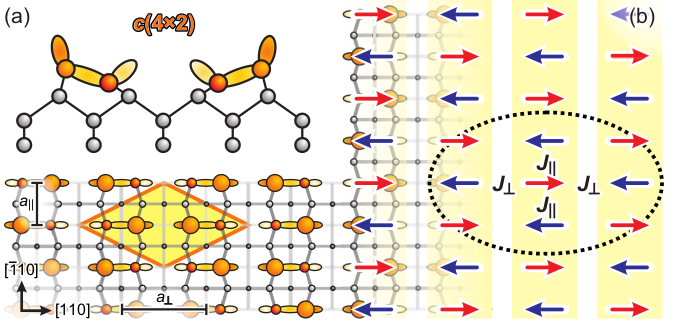
\includegraphics[width=13cm]{graphics/Silicon-System.png}
		\caption{Atomic structure model of the Si(001) surface reconstruction and a Spin model describing the arrangement of alternation of dimer buckling. Coupling energies $J_{\parallel}$ along dimer rows and $J_{\perp}$ \cite{brand2023dimer}}
	\end{figure}
	With the 2D Ising
	\begin{align}
		&T_c =	190.6 \text{K}  \\
		&\xi_{\parallel}^{\dagger}/\xi_{\perp} =	5.2 		\\
		&J_{\parallel} =	-24.9 \text{meV} \\
		&J_{\perp} = -0.8 \text{meV}
	\end{align}
	We can describe the system by mapping the anisotropic 2D Ising model on a rectangular lattice, mapping the the Ising spins $\sigma_{i,j} =	\pm 1$ on the two buckling orientations. The two dimer configurations are separated by an energy barrier $E_b \approx 90 \text{meV}$ that is large compared to the thermal fluctuations at the critical point. But what does that mean? Two Flip one spin I need to put in 90 meV? That is pretty large and why doesn't the transition just happen earlier then? This seems to mean that intermediate states get exponentially suppressed. The Hamilton of the 2D anisotropic Ising model without external field is known. It was solved by Onsager and exhibits its phase transition at
	\begin{equation}
		\sinh(\frac{2 |J_{\parallel}|}{k_B T_c}) \sinh(\frac{2 |J_{\perp}|}{k_B T_c}) =	1
	\end{equation}
	We can use that to estimate our phase transition? Or is that a whole different thing? For my tries without anisotropy The equation simplifies to
	\begin{equation}
		\sinh\left(\frac{2 |J|}{k_B T_c}\right) =	1 \qquad \Rightarrow \qquad |J| =	\frac{1}{2}k_B T_c \cdot \text{arsinh}\left(1\right)
	\end{equation}
	Oups that was the wrong umformung.
	\begin{equation}
		\sinh\left(\frac{2 |J|}{k_B T_c}\right) =	1 \qquad \Rightarrow \qquad T_c = \frac{2 |J|}{k_B ~ \text{arsinh}\left(1\right)} = 113 \qquad \text{for} \qquad J = 50
	\end{equation}
	yeah that doesn't really check out.
	Btw., the lattice spacing of the dimerized Si(001) surface are
	\begin{equation}
		a_{\parallel} =	3.84 \text{~\AA} \qquad \text{and} \qquad a_{\perp} =	2a_{\parallel} = 7.68 \text{~\AA}
	\end{equation}
	Universality we also get it's scaling with that we can approximate the scaling of the system. It is also possible to derive explicit equations for the correlation length in the different directions. It is even possible to determine the coupling strengths with the ratios of the correlation lengths, so that we can calculate them from the experiment.
	
	Because of the large correlation length anisotropy it is valid to only look at nearest neighbor couplings. But it seems that the effective $J_\perp$ actually changes sign when switching from NNN to NN. $J_\perp$ is actually positive for NNN, but the coupling to the diagonal dimers is almost as strong as the coupling to the horizontal dimer and since there are two diagonal dimers, this interaction is actually stronger. Now the Dimer between the diagonal ones couples to them with a stronger coupling strength $J_\parallel$ which is negative and therefore flips. So we have a positive $J_\perp$ for NNN and a negative one for $J_\parallel$.
	
	\subsection{Open Quantum Systems}
	The theory of open quantum systems deals with systems, that are not closed in itself (or isolated), but rather coupled to its environment, leading to different dynamics and quantum dissipation. It is based on the assumption that the density matrix of the universe (or the global density matrix), that includes the system as well as it's environment, evolves according to the von Neumann equation:
	\begin{equation}
		\frac{\text{d}{\rho_{SB}}}{\text{d}{t}} = - i \left[H_{tot}, \rho_{SB} \right]
	\end{equation}
	We usually decompose the total Hamiltonian to be $H_{tot} =	H_S + H_B + H_I$, $H_S$ describing the system hamiltonian, $H_B$ the one of the bath and $H_I$ the interaction (between the two) hamiltonian. The time evolution can also be described with the time evolution $U(t)$ operator
	\begin{equation}
		\rho_{SB}(t) =	U(t) \rho_{SB}(0) U^\dagger(t)
	\end{equation}
	Usually we are only interested in the time evolution of the system and the bath is usually taken to be large and stationary. We can obtain the density matrix of the system by performing a partial trace $\rho_S(t) =	\text{tr}_B \left\{\rho_{SB}(t)\right\}$. Every form of time evolution for $\rho$ should be completely positive and trace preserving, so that it preserves hermiticity, normalization and positivity, or in other words, that it maps density matrix to density matrix.
	
	The most general form for a differential equation that is CPTP (completely positive and trace preserving) is one of the Lindblad form:
	\begin{equation}
		\frac{\text{d} \rho_S}{\text{d}t} -i \left[H_S, \rho_S\right] + \sum_k \left(L_k \rho_S L_k^\dagger - \frac{1}{2} \left\{L_k^\dagger L_k, \rho_S \right\}\right)
	\end{equation}
	The $L_k$ are called jump operators.
	\subsubsection{Weak system-bath coupling}
	For weak system-bath coupling it is usually useful to switch to the interaction picture with respect to $H_S + H_B$ (why actually?). The von Neumann equation then reads (denoting Operators in interaction picture with \textbf{bold} symbols):
	\begin{equation}
		\dot{\boldsymbol{\rho}}_{SB}(t) =	-i \left[\mathbf{H_I}(t), \boldsymbol{\rho}_{SB}(t)\right]
	\end{equation}
	We can usually decompose $\mathbf{H_I}(t)$  as $\mathbf{H_I} =	\mathbf{A_I}(t) \otimes \mathbf{B_I}(t)$ if $H_I =	A_I \otimes B_I$ and since (per Definition? I mean they act on totally different fock spaces) $\left[H_S, H_B\right] =	0$:
	\begin{equation}
		\mathbf{H_I}(t) =	e^{i (H_S + H_B)t} H_I e^{-i (H_S + H_B)t} =	e^{i H_S t} A_I e^{- i H_S t} \otimes e^{i H_B t} B_I e^{-i H_B t} =	\mathbf{A_I}(t) \otimes \mathbf{B_I}(t)
	\end{equation}
	We can formally integrate the von Neumann equation in interaction picture with the initial condition $\boldsymbol{\rho}_{SB}(0) = \rho_{SB}(0) =	\rho_0$
	\begin{equation}
		\int_{0}^{t} \dot{\boldsymbol{\rho}}_{SB}(t') dt' =	\boldsymbol{\rho}_{SB}(t) - \rho_0 = -i \int_{0}^{t} \left[\mathbf{H_I}(t'), \boldsymbol{\rho}_{SB}(t')\right]	dt'
	\end{equation}
	solving for $\boldsymbol{\rho}_{SB}(t)$ and inserting back into von Neumann equation then yields
	\begin{equation}
		\dot{\boldsymbol{\rho}}_{SB}(t) =	-i \left[\mathbf{H_I}(t), \rho_0 \right] -\int_{0}^{t} \left[\mathbf{H_I}(t)\left[\mathbf{H_I}(t'), \boldsymbol{\rho}_{SB}(t')\right]\right]	dt'
	\end{equation}
	We are mainly interested in the time evolution of the system, so we trace out the degrees of freedom of the bath and since $\dot{\boldsymbol{\rho}}_S =	\frac{\text{d}}{\text{dt}} \boldsymbol{\rho}_S =	\frac{\text{d}}{\text{dt}} \text{tr}_B\left\{ \boldsymbol{\rho}_{SB}\right\} = \text{tr}_B\left\{ \dot{\boldsymbol{\rho}}_{SB}\right\}$:
	\begin{equation}
		\dot{\boldsymbol{\rho}}_{S}(t) =	-i ~\text{tr}_B \left\{\left[\mathbf{H_I}(t), \rho_0 \right]\right\} - \int_{0}^{t} \text{tr}_B \left\{\left[\mathbf{H_I}(t)\left[\mathbf{H_I}(t'), \boldsymbol{\rho}_{SB}(t')\right]\right]\right\}	dt'
	\end{equation}
	This equation can be closed by using the \textbf{Born Approximation} $\boldsymbol{\rho}_{SB} =	\boldsymbol{\rho}_S(t) \otimes \overline{\rho}_B$, which basically states that the bath is in a constant state that does not change.
	\subsubsection{Quantum Brownian Motion}
	In the Setting
	\begin{equation}
		H_S = \frac{1}{2m} p^2 + V(x) \qquad H_B =	\sum_k \omega_k b_k^\dagger b_k \qquad H_{SB} =	- x \otimes \sum_k h_k x_k
	\end{equation}
	One can derive in the limit for fast decaying correlation functions with respect to the relaxation time of the combined system and with respect with the relaxation time of the considered system, so
	\begin{equation}
		\tau_{Bath} \ll \tau_{Combined} \qquad \wedge \qquad \tau_{Bath} \ll \tau_{System}
	\end{equation}
	the \textbf{Caldeira-Leggett Master equation} that looks like \cite{breuer2002theory}
	\begin{equation}
		\frac{d}{dt} \rho_S(t) =	- i \left[H_S, \rho_{S}(t)\right] - i \frac{\eta}{2} \left[x, \left\{ p, \rho_S(t) \right\}\right] - { \eta k_B T} \left[x, \left[x, \rho_S(t)\right]\right]
	\end{equation}
	The Caldeira-Leggett Master equation is not in Lindblad form so it is not CPTP, but it can be brought to Lindblad form by adding a term that is small in the high-temperature limit.
	From the Caldeira-Leggett Master equation one can derive equations of motions for the mean values the usual way. For Moments of $x$ and $p$ one obtains:
	\begin{align}
		\frac{d}{dt}\langle x \rangle &= \frac{1}{m} \langle p \rangle \\
		\frac{d}{dt}\langle p \rangle &=	- \langle V'(x)\rangle -  \eta \langle p \rangle \\
		\frac{d}{dt} \langle x^2 \rangle &= \frac{1}{m} \langle px + xp \rangle \\
		\frac{d}{dt} \langle p^2 \rangle &=	- \langle p V'(x) + V'(x)p \rangle - 2 \eta \langle p^2 \rangle + 2 \eta k_B	T
	\end{align}
	We can compare those to the differential equations arising form classical brownian motion (in a potential) (or rather the Ornstein- Uhlenbeck process!)
	\begin{align}
		\frac{d}{dt} \langle p(t) \rangle &=	- \eta \langle p(t) \rangle \\
		\frac{d}{dt} \langle p^2(t) \rangle &= - 2 \eta \langle p^2(t) \rangle + 2 \eta k_B T
	\end{align}
	The latter term in the equation for the second moment of $p$ corresponds to the diffusion function of the Langevin equation. The equations for the means look the same so we can identify the classical pendant to the quantum mechanical mean ODEs are the langevin-equations (or stochastic differential equations)
	\begin{align}
		\frac{d}{dt} x(t) &=	p(t) \\
		\frac{d}{dt} p(t) &= - \frac{d}{dx} V(x) - \eta p(t) + \sqrt{2 \eta k_B T} ~ \Gamma (t)
	\end{align}
	Which are analog to the stochastic differential equations in section numerical methods.¸
	\section{Model}
	\subsection{Potential}
	We assume the Dimers live in a double well potential of the form:
	\begin{equation}
		V(q) = \frac{1}{2}	\alpha \left(q^4 - \beta q^2 \right) \qquad \text{with} \qquad \alpha, \beta > 0
	\end{equation}
	The force acting on a lone Dimers is then
	\begin{equation}
		F(q) =	\frac{\partial V}{\partial q} =	\alpha \left(2q^3 - \beta q \right)
	\end{equation}
	The potential has its maximums and minimums where
	\begin{equation}
		F(q^*) = 0 \qquad \Rightarrow \qquad 2(q^*)^3 =	\beta q^* \qquad \Rightarrow \qquad q^*_\pm = \pm	\sqrt{\frac{\beta}{2}} \quad \text{or} \quad q^*_0 = 0
	\end{equation}
	
	Since $V(q^*_0) = 0$, the energy difference between minimum and maximum is
	\begin{equation}
		|V(q^*_\pm)| =	- \frac{1}{2}\alpha \left((q^*_\pm)^4 - \beta (q^*_\pm)^2\right) =  -\frac{1}{2}\alpha \left(\left(\sqrt{\frac{\beta}{2}}\right)^4 - \beta \left(\sqrt{\frac{\beta}{2}}\right)^2\right)	=	\frac{1}{8} \alpha \beta^2
	\end{equation}
	A graph of the potential is shown in ...
	\begin{figure}
		\centering´
		\includegraphics[width=12cm]{graphics/potential.png}
	\end{figure}
	A reasonable assumption would be to suspect that the phase transition occurs when $|V(q^*_\pm)|$ is approximately as large as the thermic energy. For a single particle moving in \textbf{1D} in a bath of Temperature $T$, its average kinetic energy should be
	\begin{equation}
		\langle E_{\text{kin}} \rangle = \frac{1}{2} k_B T
	\end{equation}$\alpha$
	
	meaning the critical temperature $T_c$ should be around
	\begin{equation}
		\langle E_{\text{kin}} \rangle (T_c) \approx |V(q^*_\pm)| \qquad \Rightarrow \qquad T_c(\alpha, \beta) \approx \frac{1}{4} \frac{\alpha \beta^2}{k_B}
	\end{equation}
	
	I just did a sweep with the values $\alpha = 1$ and $\beta = 10$, which means the critical temperature should be around $T_c \approx 25$ (natural units). My usual parameters were $\alpha = 5$ and $\beta = 10$, which means the phase transition should have happened at $T_c \approx 125$, which was not the case I think.
	
	I just saw that the value of $T_c$ was heavily influenced by the kind of Interaction in used. So the strength of the interaction also has to be taken into account. But i actually don't really know how i would do this.
	
	Maybe kinetic energy should be of the same order as energy of the combined potential?
	But if they are aligned, the Interaction potential actually has a value of 0.
	
	\begin{center}
		\begin{tabular}{c|c|c|c}
			\centering
			$\alpha$ & $\beta$ & $T_c^{\text{theo}}$ & $T_c^{\text{actual}}$ \\  [0.5ex]
			\hline
			1 & 10 & 25 & ?	\\
			5 & 10 & 125 & 40 \\
			5 & 20 &
		\end{tabular}
	\end{center}
	
	For a quadratic potential, the Interaction Energy between a dimer and its neighbors, if all its neighbors sit in the right minimum is:
	\begin{equation}
		\begin{split}
			V_I (\lbrace q_{i, j} \rbrace_{NN^+}) &= \frac{1}{2}	\alpha \left(q_{i, j}^4 - \beta q_{i, j}^2 \right)&+ J_{\parallel}/2 \left(\left( q_{i, j} - q^*_+   \right)^2 + \left(q_{i, j} - q^*_+\right)^2 \right)\\
			&~&+ J_{\perp}/2 \left(\left( q_{i, j} - q^*_+   \right)^2 + \left(    q_{i, j} - q^*_+\right)^2 \right)\\
			&\overset{J_\parallel =	J_\perp}{=} \frac{1}{2}	\alpha \left(q_{i, j}^4 - \beta q_{i, j}^2 \right)&+ 2J \left( q_{i, j} -\sqrt{\frac{\beta}{2}}   \right)^2 \\
		\end{split}
	\end{equation}
	This potential has its minima at:
	\begin{equation}
		F(q_{i, j}) =	\frac{\partial 	V_I (\lbrace q_{i, j} \rbrace_{NN^+})}{\partial q_{i, j}} =	\alpha \left(2q_{i, j}^3 - \beta q_{i, j} \right) + 4 J	\left( q_{i, j} -\sqrt{\frac{\beta}{2}}   \right) =	0
	\end{equation}
	It has one trivial minimum at $q_{i, j} = \sqrt{\frac{\beta}{2}}$ and another one depending on $\alpha, \beta, J$. This minimum exists approximately if $J < \frac{1}{17} 	\alpha  \beta$. We want it to exist, since otherwise we are very likely to see only one phase in the system.
	
	\subsubsection{Damping in potential}
	For motion in a harmonic potential one can classify the over- and underdamped regime. To get a feeling for the motion our system performs, we assume that we are most of the time located around one of the minima of the potential. In the Minimum, we can taylor the double well potential to second order to get a harmonic potential that approximates the $q^4$ potential around the minimum. We can then classify whether our system is approximately in the over- or underdamped case and get a feeling for the motion.
	
	Since we want to taylor around the minimum, the first derivative of the potential is $\frac{\partial V}{\partial q} =	0$ and we can write the second order taylor expansion as
	\begin{equation}
		T_2 V(q, q^*_\pm) =	V(q^*_\pm) + \left(q -q^*_\pm \right)^2 \frac{\partial^2 V}{\partial^2 q} \Big |_{q^+_\pm} =	- \frac{1}{8} \alpha \beta^2 + 2 \alpha \beta \left(q -q^*_\pm \right)^2
	\end{equation}
	Which means the dynamics around our minima should behave similar to the dynamics of a harmonic potential with the spring constant $k =	4 \alpha \beta$. Therefore the critical dampening is
	\begin{equation}
		\eta_c =	2 \sqrt{k} =	4 \sqrt{\alpha \beta}
	\end{equation}
	The damping ratio $\zeta =	\frac{\eta}{\eta_c}$ describes whether we are underdamped $\zeta < 1$ or overdamped $\zeta > 1$.
	\begin{center}
		\begin{tabular}{ c c c c c c}
			$\alpha$ & $\beta$& $\eta$ & $\eta_c$ & $\zeta$ & Equil. time \\
			\hline
			10 & 1 & 1.5  & 12.64 & 0.12 & > $10^4$\\
		\end{tabular}
	\end{center}
	Turns out probably all my runs were done in heavily underdamped case. This could be the reason for slow equilibration, but could also be not significant at all. We should do some simulations and somehow think of a criteria for equilibration. I think the ''goodness-of-intersection'' or the form of the derivative of a phenomenological coupling could be some inidicators.
	\subsection{System}
	We already described the physical system, now we describe our model for this system. Since we have inclined Dimers in the real physical system, it would be reasonable to use the inclination angle as coordinate. Our Dimers have no arrowheads, which means, our Inclination angle only reaches from $ \left[-\frac{\pi}{2}, ~\frac{\pi}{2}\right)$. The inclination angle is therefore limited in contrast to the conjugated coordinate of the potential in the last section. This means we need to have some kind of transformation $f:	\left[-\frac{\pi}{2}, ~\frac{\pi}{2}\right) \rightarrow \mathbb{R}, \quad \vartheta \rightarrow f(\vartheta)$. Such a Transformation would be
	\begin{figure}
		\centering
		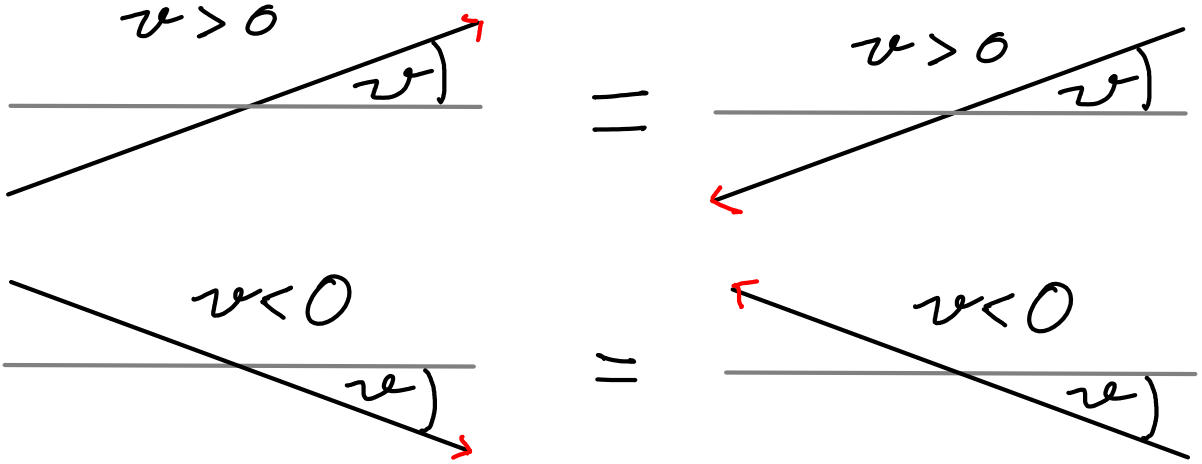
\includegraphics[width=10cm]{graphics/coordinate.png}
	\end{figure}
	\begin{equation}
		f(\vartheta) =	a \cdot \text{arctanh}\left(\frac{2 \vartheta}{\pi}\right)
	\end{equation}
	With this our cosine interaction doesn't make to much sense anymore?
	
	With this transformation the back transformation would be
	\begin{equation}
		\vartheta(q) =	\frac{\pi}{2} \tanh\left(\frac{q}{a}\right)
	\end{equation}
	\subsection{Interaction}
	The plan now would be to calculate with $q$ and plot $\theta$.
	Since the maximum inclination angle difference is $\Delta \vartheta =	\pi$, we could also use a linear interaction potential like
	\begin{equation}
		V_I(\vartheta_1, \vartheta_2) = J \cdot \left(\pi - |\vartheta_1 - \vartheta_2|\right) \qquad \text{or}	\qquad  V_I(\vartheta_1, \vartheta_2) = J \cdot \left(\pi^2 - (\vartheta_1 - \vartheta_2)^2 \right)
	\end{equation}
	Here ($J > 0$) for larger $\Delta \vartheta$, we have a smaller Interaction Energy and therefore the antisymmetric alignment would be favored. The first one would result in a constant force, which is probably not what we want. If I am doing the simulation with q, probably the force would be
	\begin{equation}
		F_I(\vartheta_1(q_1), \vartheta_2(q_2)) = \frac{\partial V_I(\vartheta_1(q_1), \vartheta_2(q_2))}{\partial q_1} =	\frac{\partial V_I(q_1, q_2)}{\partial q_1}
	\end{equation}
	Or is it just
	\begin{equation}
		F_I(\vartheta_1(q_1), \vartheta_2(q_2)) =	\frac{\partial V_I(\vartheta_1, \vartheta_2)}{\partial \vartheta_1}
	\end{equation}
	And then replace the $\vartheta$ with the $q$? $\Rightarrow$ depends on the differential equation we are looking at. I want to deal with the SDE for the transformed coordinate $q$, so will have to differentiate for $q$.
	
	The current implementation uses an Interaction which is based on the cosine:
	\begin{equation}
		V_I(\vartheta_1, \vartheta_2) =	J \cdot (1 - \cos\left(\theta_1 - \vartheta_2\right)) \qquad \Rightarrow \qquad F_I(\vartheta_1, \vartheta_2) = J	\cdot \sin\left(\vartheta_1 - \vartheta_2\right)
	\end{equation}
	This potential also has the the absolute value of $V_I$ is the smallest for $\vartheta_1 =	\vartheta_2$ and largest for $\Delta \varphi =	\pi$. Depending on the sign of J, this means either ferromagnetic ($J>0$) or antiferromagnetic ($J < 0$) interaction.
	
	\textbf{Important realization:} I am currently using the transformed coordinates $q$ to calculate the interaction, which is totally wrong, since cosine is periodic and for a difference of $\Delta q > \pi$ (which is totally possible), the direction of the interaction changes sign.
	\begin{figure}
		\centering
		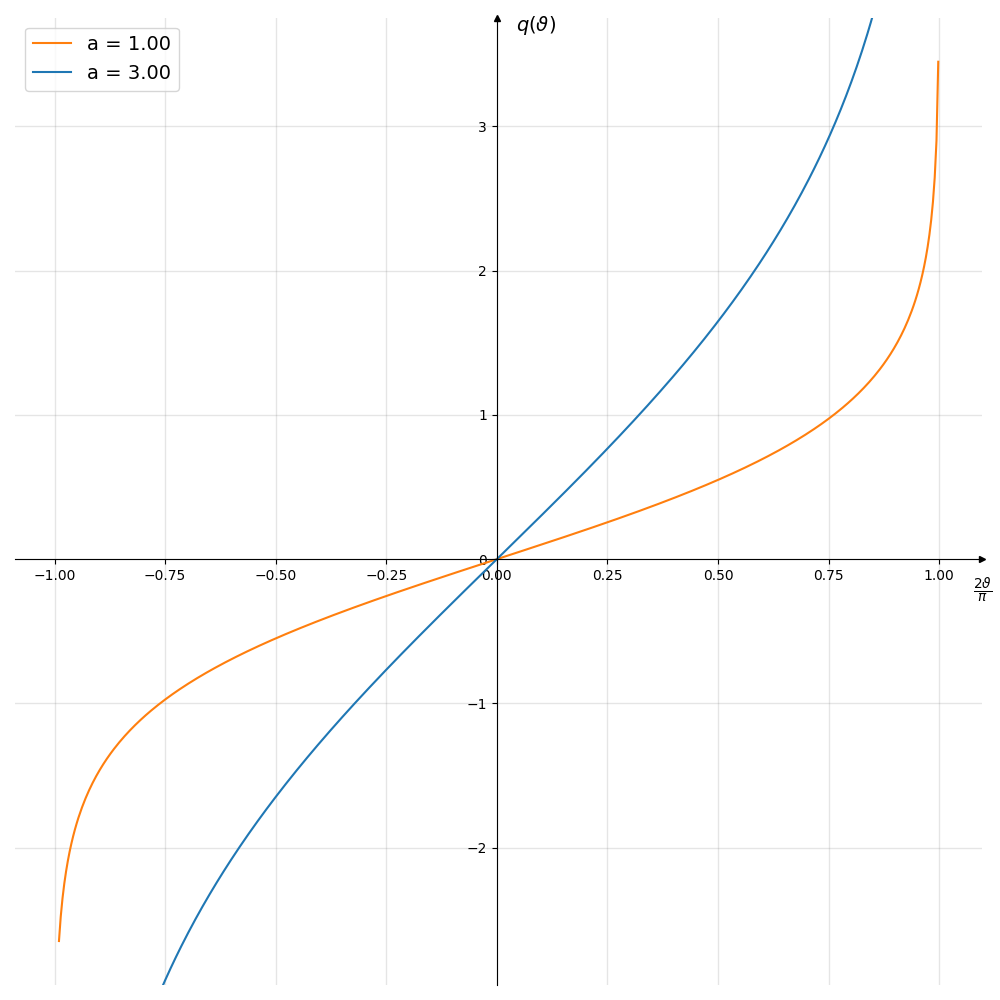
\includegraphics[width=12cm]{graphics/coordinate-trafo.png}
	\end{figure}
	So we need another Interaction potential. The thing is, if we choose a quadratic potential:
	\begin{equation}
		V_I (q_1, q_2) = \frac{J}{2} \cdot (q_1 - q_2) ^2 \qquad \Rightarrow \qquad F_I (q_1, q_2) = J \cdot (q_1 - q_2)
	\end{equation}
	This term can get arbitrarily large if we increase the $\Delta q$. I am thinking about a situation in anitferromagnetic interaction where the dimers run away from each other to infinity. But I think that should be suppressed by th $q^4$ potential, which rises faster than the Interaction potential.
	
	In terms of NN	Interaction the whole potential would look like this:
	\begin{align}
		V_I (\lbrace q_{i, j} \rbrace_{NN}) =	~~&J_{\parallel}/2 \left(\left( q_{i, j} - q_{i, j-1}   \right)^2 + \left(    q_{i, j} - q_{i, j+1}\right)^2 \right) \\
		+ &J_{\perp}/2 \left(\left( q_{i, j} - q_{i-1, j}   \right)^2 + \left(    q_{i, j} - q_{i+1, j}\right)^2 \right)
	\end{align}
	And therefore the force:
	\begin{align}
		\frac{\partial V_I(\lbrace q_{i, j} \rbrace_{NN})}{\partial q_{i, j}} =	~~&J_{\parallel} \left(\left( q_{i, j} - q_{i, j-1}   \right) + \left(    q_{i, j} - q_{i, j+1}\right) \right) \\
		+ &J_{\perp} \left(\left( q_{i, j} - q_{i-1, j}   \right) + \left(    q_{i, j} - q_{i+1, j}\right) \right)
	\end{align}
	\subsubsection{Coulomb Interaction}
	We could also imagine our particles to be charged and confined to a rail pointing in z-direction. In this z-direction there is also the double well potential which makes the bistable potential. The particles are of opposite or same charge and therefore want to order ferromagnetic or antiferromagnetic. The rails sit on designated positions in the X-Y-plane, and therefore with lattice spacings $a_x, a_y$, the coulomb interaction energy between two sites will be
	\begin{equation}
		V_I (q_{i,j}, q_{i+q, j+s}) =	\frac{C}{\sqrt{(q a_x)^2 + (s a_y)^2 + (q_{i, j} - q_{i+q, j+s})^2}}
	\end{equation}
	The Dimension of C is $[C] = \text{J} \cdot \text{m}$.
	This interaction is ferromagnetic for $C < 0$ and antiferromagnetic for $C > 0$. For the antiferromagnetic case, the interaction term tends to be minimized, this happens by making the distance between the particles very large. Asymptotically the interaction energy vanishes $\left(\Delta q \rightarrow \infty \Rightarrow V_I \rightarrow 0\right)$. For the ferromagnetic case, the particles are attracting and the interaction term tends to be maximized. This happens by minimizing the distance between the particles $\left(\Delta q \rightarrow 0 \Rightarrow V_I \rightarrow \frac{C}{\sqrt{(q a_x)^2 + (s a_y)^2}} =	C^*\right)$. In the ferromagnetic case, in the equilibrium the interaction term will be an additive constant to the double well potential, not changing the position of our dips. In the antiferromagnetic case, the interaction does not vanish in the dips of the bistable potential, potentially moving the equilibrium positions to slightly higher q. More on this might be investigated later, we would have to minimize the potential for $q_{i, j}$, the rest of the system being in equilibrium (probably).
	
	With $d_{xy}(q, s) =(q a_x)^2 + (s a_y)^2	$, the Taylor expansion of the coulomb interaction for small differences in z-direction is
	\begin{equation}
		V_I (q_{i,j}, q_{i+q, j+s}) =	C \left(\frac{1}{d_{xy}} - \frac{(q_{i,j}-q_{i+q, j+s})^2}{2 \left(d_{xy}\right)^{3}} + ... \right)
	\end{equation}
	which is basically the quadratic interaction from above, this lets us expect similar behavior and motivates the benchmarking of quadratic interaction.
	
	The force acting between two particles will then be
	\begin{equation}
		\frac{\partial V_I (q_{i,j}, q_{i+q, j+s})}{\partial q_{i, j}} =	- C \left(\frac{(q_{i, j} - q_{i+q, j+s})}{\left((q a_x)^2 + (s a_y)^2 + (q_{i, j} - q_{i+q, j+s})^2\right)^{3/2}}\right)
	\end{equation}
	
	
	\subsubsection{Dipole-Dipole Interaction}
	Another interaction that would reproduce the behavior of the real system would be a dipole-dipole interaction between the dimers. Let's assume that the dimers have a permanent dipole moment $\vec{p} =	q \cdot \vec{d}$ that is somehow induced by the lattice. Whether this is justifiable shall be discussed later. $d =	|\vec{d}|$ will be the fixed bond length of the dimer, which is approximately known from theoretical calculations \cite{ramstad1995theoretical}. $q$ is the charge of one silicon atom in the dimer. The equilibrium angles will be
	\begin{equation}
		\vartheta_{r} =	18.8^\circ \qquad \text{and} \qquad \vartheta_{l} = (180 - 18.8)^\circ
	\end{equation}
	For a dimer pointing up right and up left respectively. We assume without loss of generality that the upper silicon atom is positively charged. The interaction energy of two electrical dipoles separated by $\vec{r}$ is
	\begin{equation}
		E(\vec{p}_1, \vec{p}_2, \vec{r}) =	\frac{\vec{p}_1 \cdot \vec{p}_2 - 3 \left(\vec{p}_1 \cdot \hat{r} \right) \left(\vec{p}_2 \cdot \hat{r}\right)}{|\vec{r}|^3}
	\end{equation}
	If we fix one dimer $\vec{p}_1$ in the upper right equilibrium position and parametrize the moment of the neighboring dimer (see \autoref{dipoleansatz}):
	\begin{equation}
		\vec{p}_2 = \left(\begin{array}{c}
			\sin \varphi \\
			\cos \varphi \\
			0
		\end{array} \right)
	\end{equation}
	\begin{figure}[htb]
		\centering
		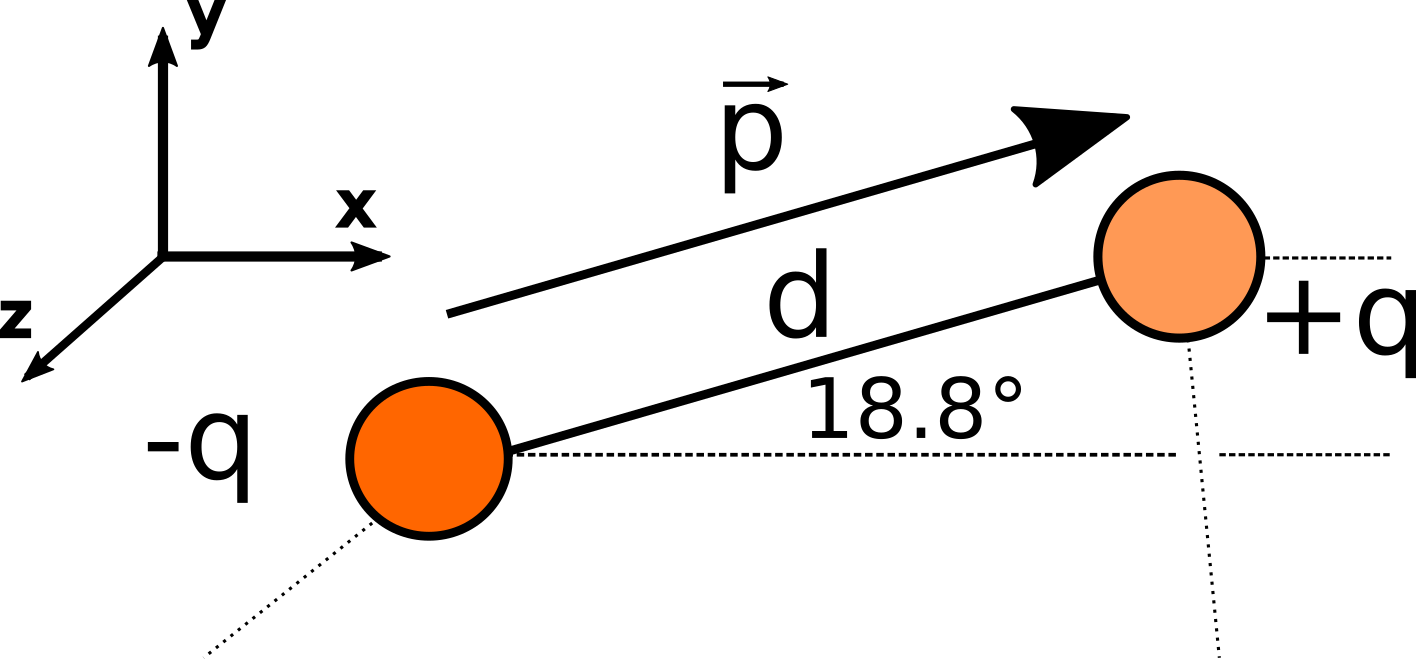
\includegraphics[width=10cm]{graphics/dipole-ansatz.png}
		\caption{dimer ansatz}
		\label{dipoleansatz}
	\end{figure}
	we can minimize the interaction energy depending on $\varphi$. Considering next nearest neighbors, we would consider interaction energies in 3 different directions (see \autoref{dipole4x2})
	\begin{equation}
		\vec{r}_x =	\left(\begin{array}{c}
			2 a \\
			0 \\
			0
		\end{array} \right)\qquad  	\qquad
		\vec{r}_{xz} =	\left( \begin{array}{c}
			2 a \\
			0 \\
			a
		\end{array} \right) \qquad 		\qquad
		\vec{r}_x =	\left(\begin{array}{c}
			0 \\
			0 \\
			a
		\end{array} \right)
	\end{equation}
	and their counterpart directions. The angle $\varphi$ that minimizes the interaction energy (obviously) depends on the direction of $\vec{r}$. For the three directions we calculate the minimal angles to be:
	\begin{equation}
		\varphi_x =	-9.7^\circ \qquad \qquad \varphi_z = 198.8^\circ \text{(just flipped)} \qquad \varphi_{xz} < 0 \text{(mistake in calc)}
	\end{equation}
	So fixing the first dipole moment to point to the upper right, the favored position of a dipole in $\vec{r}_x$ direction would also be upper right. Same goes for $\vec{r}_{xz}$ direction. In $\vec{r_z}$ direction a dipole moment flip would minimize the dipole interaction energy, meaning that the dipole pointing upper left would be favored over an aligned one.
	\begin{figure}[htb]
		\begin{subfigure}{0.5\textwidth}
			\centering
			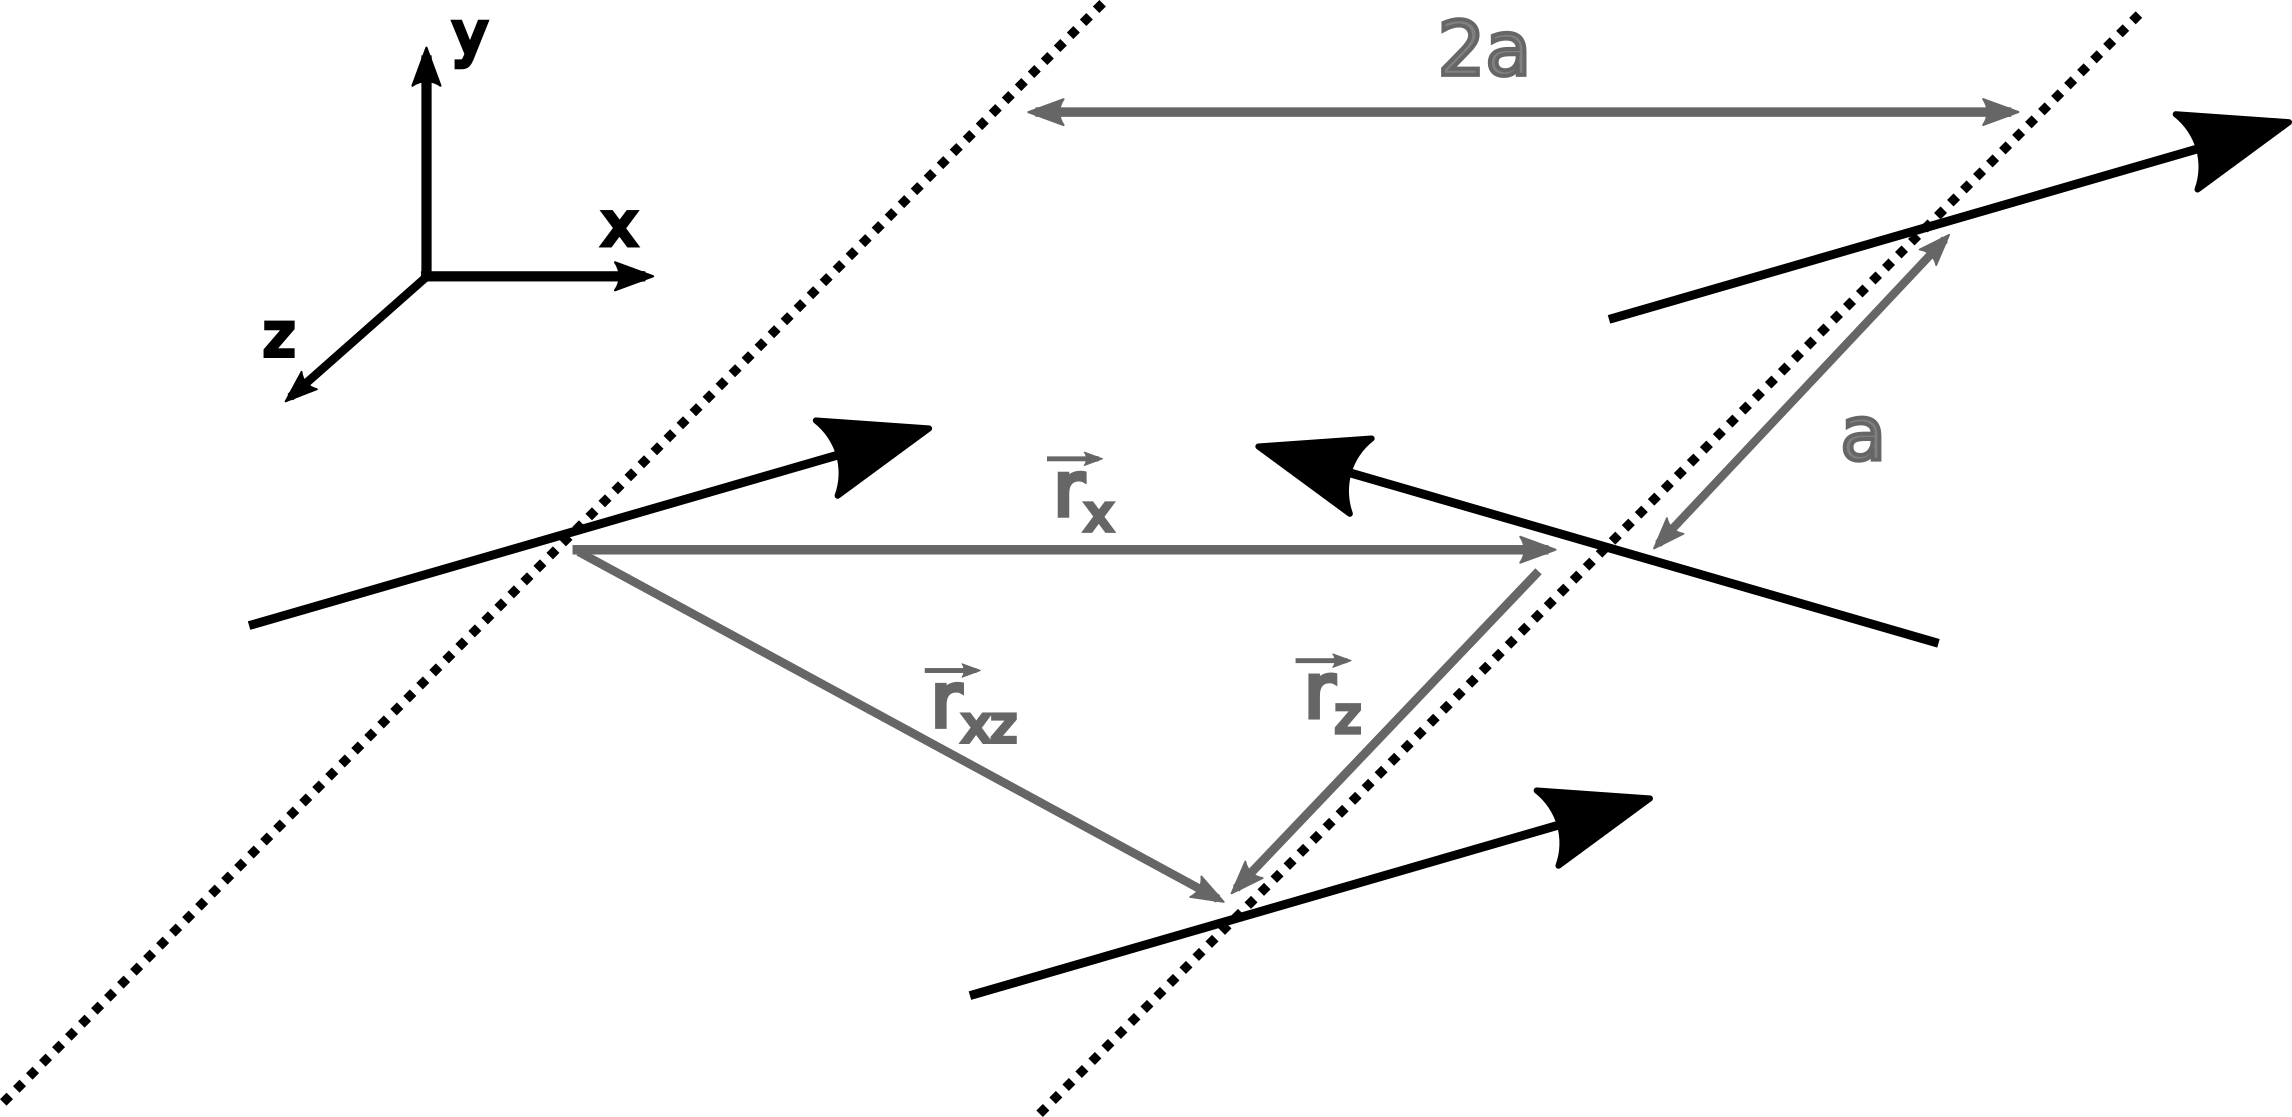
\includegraphics[width=0.8\textwidth]{graphics/c(4x2)-dipole.png}
			\caption{c(4x2) config with dipoles}
			\label{dipole4x2}
		\end{subfigure}
		\begin{subfigure}{0.5\textwidth}
			\centering
			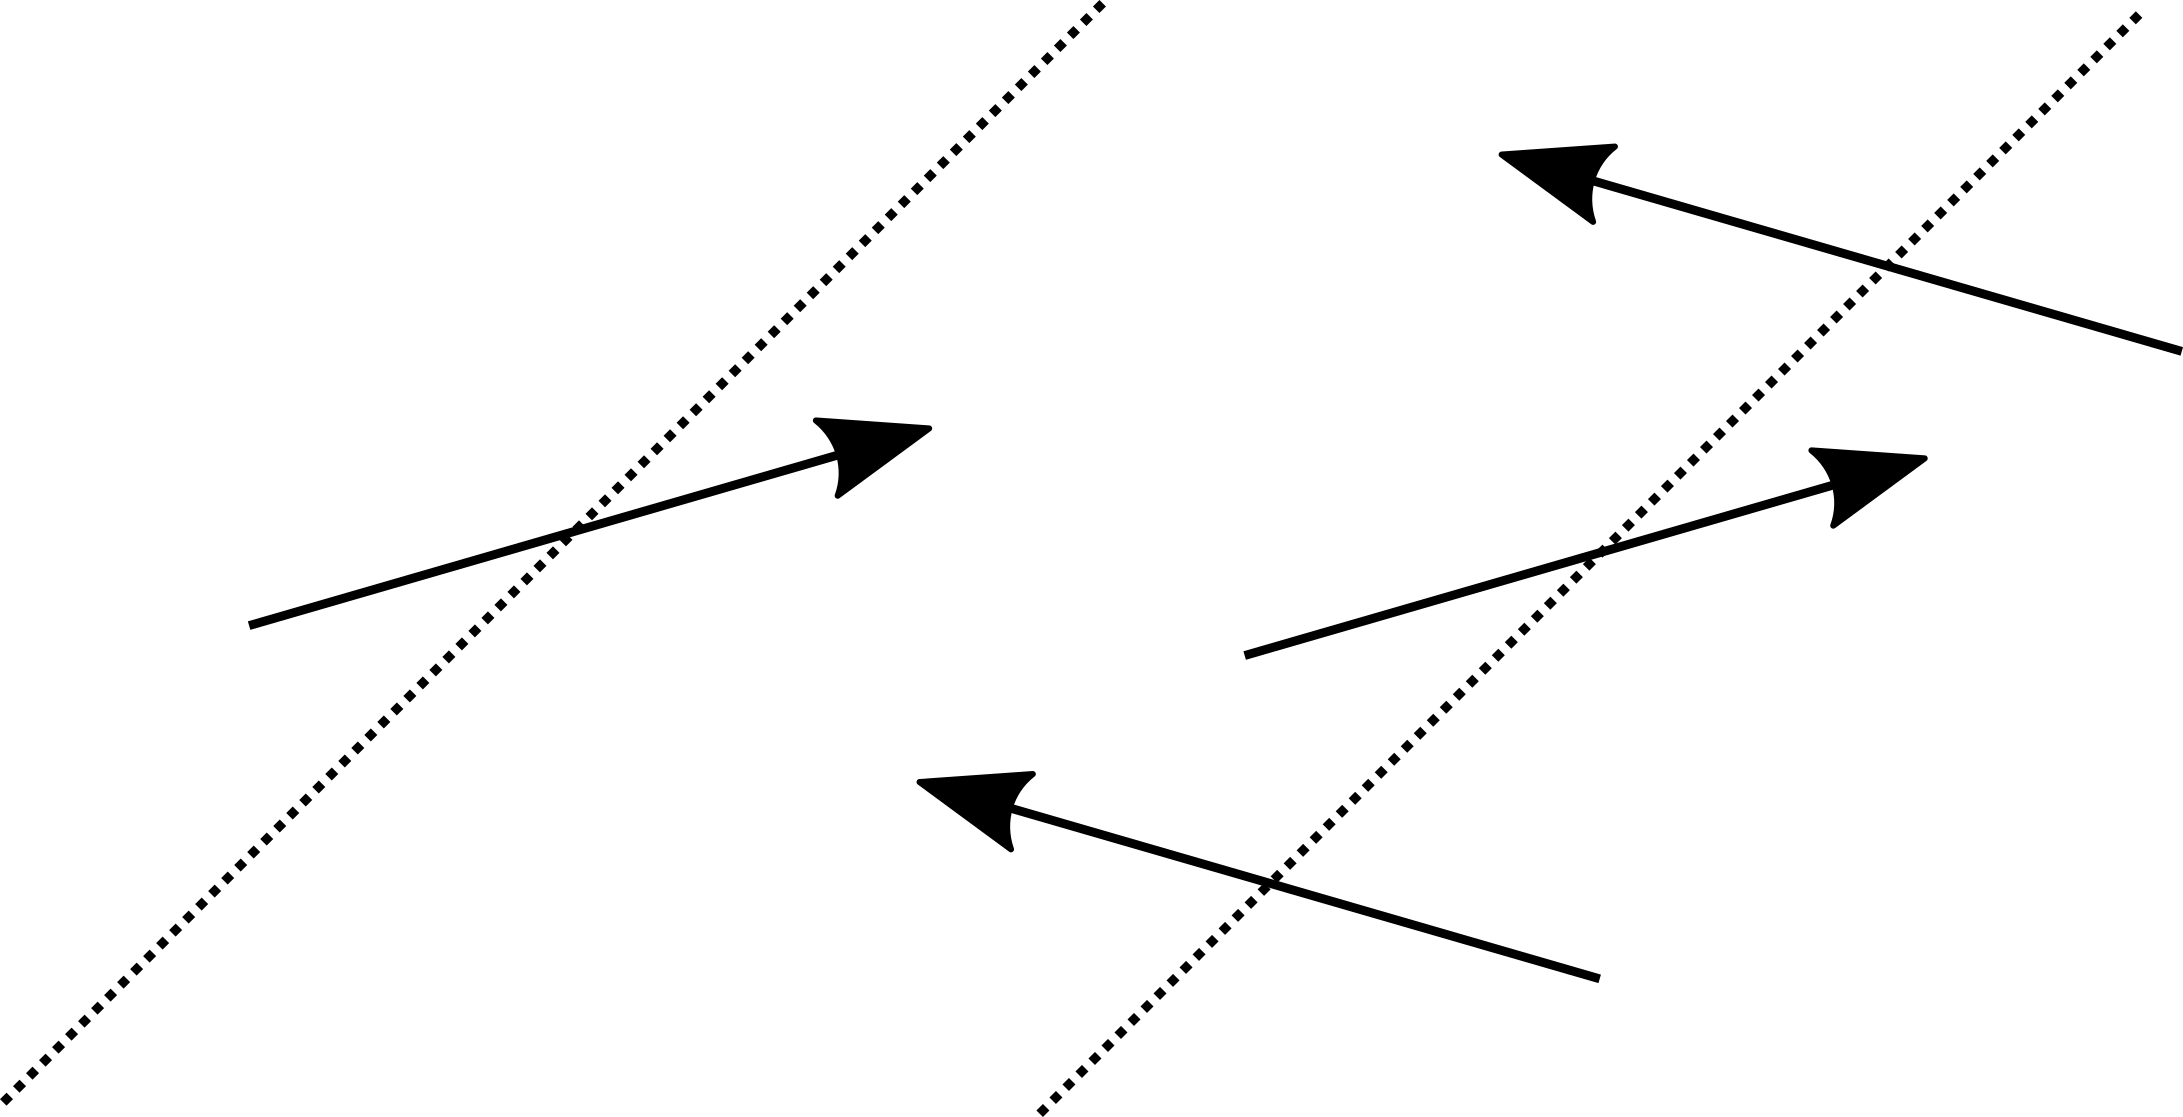
\includegraphics[width=0.8\textwidth]{graphics/2x2-dipole.png}
			\caption{p(2x2) config with dipoles}
			\label{dipole2x2}
		\end{subfigure}
		\caption{the two different possible configs}
		\label{dimer-configs}
	\end{figure}
	Calculating the total interaction energy between a fixed dipole and two different triplets, one representing the c(4x2)-reconstruction and one the p(2x2)-reconstruction shows that the c(4x2) has a slightly lower energy, just as was found in other theoretical calculations. Also the interaction across dimer rows is actually attractive, but becomes effectively repulsive in the nearest neighbor approximation. Those might be indicators that the dipole-dipole interaction might be a worth to think about?
	
	\textbf{Parameterization:}
	
	The idea was to not use a double well potential, but just a harmonic potential. That won't be suitable for the dipole-dipole interaction since the minimum would be at $\vartheta = 0$ and so we would have to measure the angle from the x-axis like in \autoref{DimerAxes}(1), so that the minimum corresponds to the $\rightarrow$-state. The Problem then would be that we have a polarization flip at $\vartheta = 0$, so $\vartheta > 0$ corresponds to a $\nearrow$-state and $\vartheta < 0$ to a $\nwarrow$-state. Which means that the total equilibrium position for two dimers along a dimer row would be $\vartheta_1 =	\varepsilon$ and $\vartheta_2 =	- \varepsilon$, so they would be flipped but still infinitesimal close to the harmonic minimum, meaning we could not reproduce the equilibrium angle of the Si(001)-surface. Also we would have to change the parameterization of the dipole moment depending on the sign:
	\begin{equation}
		\vec{p} =	l  Q \left(\begin{array}{c}
			\cos \vartheta \\
			0 \\
			\sin \vartheta
		\end{array} \right) \quad \text{for} \quad \vartheta > 0 \qquad \text{and} \qquad \vec{p} = l  Q	\left(\begin{array}{c}
			\cos \vartheta \\
			0 \\
			- \sin \vartheta
		\end{array} \right) \quad \text{for} \quad \vartheta < 0
	\end{equation}
	\begin{figure}[htp]
		\centering
		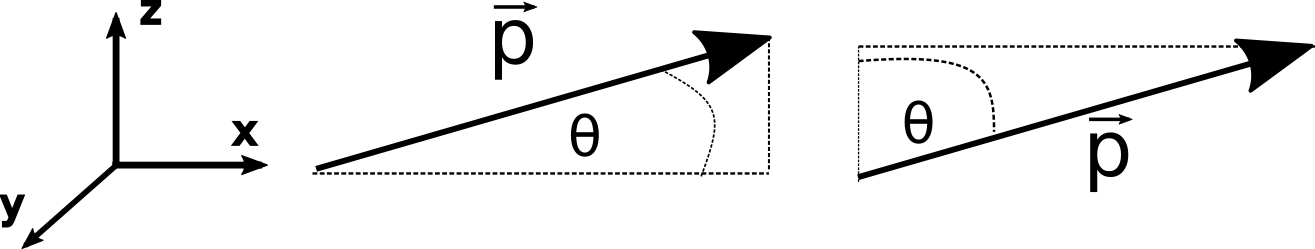
\includegraphics[width=0.8\linewidth]{graphics/DimerAngleParameterization.png}
		\caption{Possible Axes to measure the dimer buckling angle}
		\label{DimerAxes}
	\end{figure}
	Measuring from the z-Axis would provide the desired behavior, since the dipoles would repel and try to gain antiparallel configuration, at some point, which would be tuned to be at the equilibrium angle, the harmonic part would overcome the interaction potential and the dimers would stop rotating. But this would mean that the on-site potential had a minimum at a $\uparrow$-state, which is not realistic. Also the whole dynamic would take place around this state, which probably does not happen in the real system. Measuring from the z-axis, the dipole moment does not depend on the sign of the angle:
	\begin{equation}
		\vec{p} =	lQ\left( \begin{array}{c}
			\sin \vartheta \\
			0 \\
			\cos \vartheta
		\end{array} \right)
	\end{equation}
	So a description with a harmonic potential is probably not suitable, which means we turn to a bistable potential again. There are two choices: (I) ordinary double well potential which would have to be reparameterized in case (2) since we want the walls to be around the $\vartheta =	0$ location. (II) cos-like potential like in the upcoming case with the XY-model with anisotropic perturbations, see \autoref{DipolOnsite}.
	\begin{figure}[htp]
		\begin{subfigure}{0.5\textwidth}
			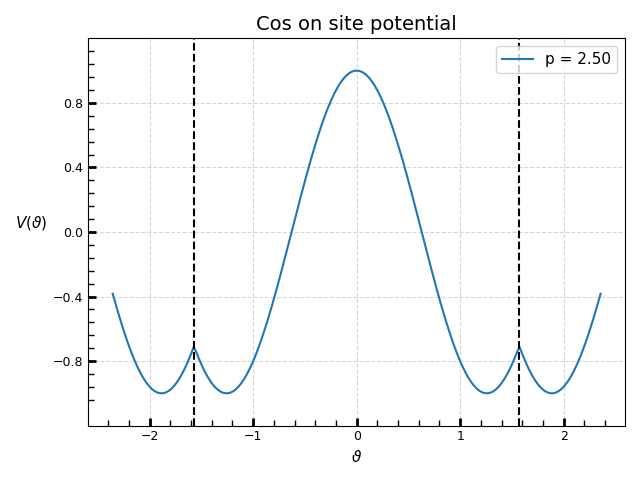
\includegraphics[width=0.8 \linewidth]{graphics/CosOnSite.png}
		\end{subfigure}
		\begin{subfigure}{0.5\textwidth}
			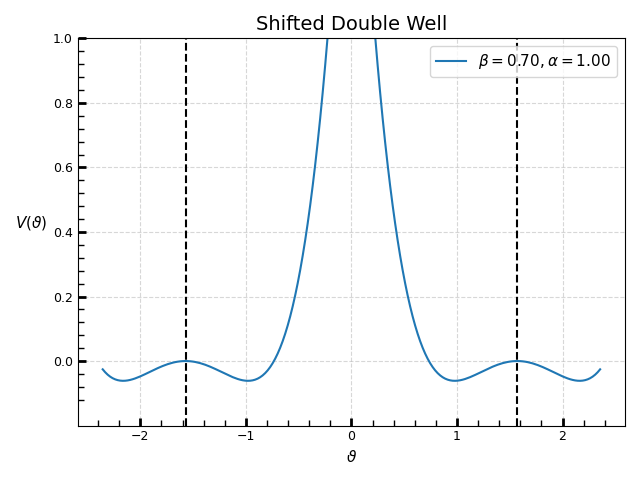
\includegraphics[width=0.8 \linewidth]{graphics/ShiftedDoubleWell.png}
		\end{subfigure}
		\caption{Possible On site potentials form z-axis angle parameterization}
		\label{DipolOnsite}
	\end{figure}
	The third possibility would be to use the x-axis parameterization and use the usual centered double well, but then we would have to calculate the Interaction depending on the sign of $\vartheta$.
	
	If we use the angle as order parameter, we need to adapt our equations of motion to rotational motion. The time derivative of the buckling angle of the dimer is the angular velocity, which is a vector. Our dimer is only allowed to rotate in the x-z-plane, so only the y-component of the \textbf{angular velocity} is relevant, since this is the component that describes the rotation around the y-axis:
	\begin{equation}
		\dot{\vartheta} =	\vec{\omega} \hat{e}_y
	\end{equation}
	The change in time of the \textbf{angular velocity} is described by the \textbf{angular acceleration} $\vec{\alpha}$.
	\begin{equation}
		\dot{\vec{\omega}} =	\vec{\alpha}
	\end{equation}
	The angular acceleration results out of an applied \textbf{torque} $\vec{\tau}$ and scales with the \textbf{moment of intertia} $I$.
	\begin{equation}
		\vec{\alpha}=	\frac{1}{I} \vec{\tau}
	\end{equation}
	The torque on a dimer in the field of another dimer is given by
	\begin{equation}
		\vec{\tau}(\vec{p}_1, \vec{p}_2, \vec{r}) =	\vec{p}_2 \times \vec{E}(\vec{p_2}, \vec{r})
	\end{equation}
	$\vec{E}$ being the electric field that the second dipole induces at the position of the first dipole $\vec{r}$. For a general force that acts at the position $\vec{r}$, the resulting torque is
	\begin{equation}
		\vec{\tau} =	\vec{r} \times \vec{F}
	\end{equation}
	If we want to calculate a torque out of the on-site potential, we have to determine where the force acts and then use
	\begin{equation}
		\vec{F} =	- \nabla V
	\end{equation}
	If the potential is only dependent on the angle $\vartheta$, we can rewrite the $\nabla$-operator in cylinder coordinates and the force becomes
	\begin{equation}
		\vec{F}(\rho, \vartheta) =	 - \frac{1}{\rho}  \vec{e}_\vartheta \frac{\partial}{\partial \vartheta} V(\vartheta).
	\end{equation}
	$\rho$ is in this case the distance from the chosen coordinate system origin at which we calculate the derivative. In case of the dimers, we can for example postulate that the force attacks at the silicon atoms at that the kos origin is in the center of the dimer. The force generated by a potential that is only dependent on an angle has to decrease with the distance to the origin, as you have to transverse a greater distance to get from $\vartheta_1$ to $\vartheta_2$ if you are located further outside. So the derivative in real space has to become smaller since the slope of the V values increases. Since the torque scales with the radius at which it attacks and the force scales with the inverse radius, the radius in the end cancels out.
	
	We could also parameterize the dipole-moment with the z-Value of the right Silicon atom of the dimer, see \autoref{DipoleQParameterization}.
	\begin{figure}[htp]
		\centering
		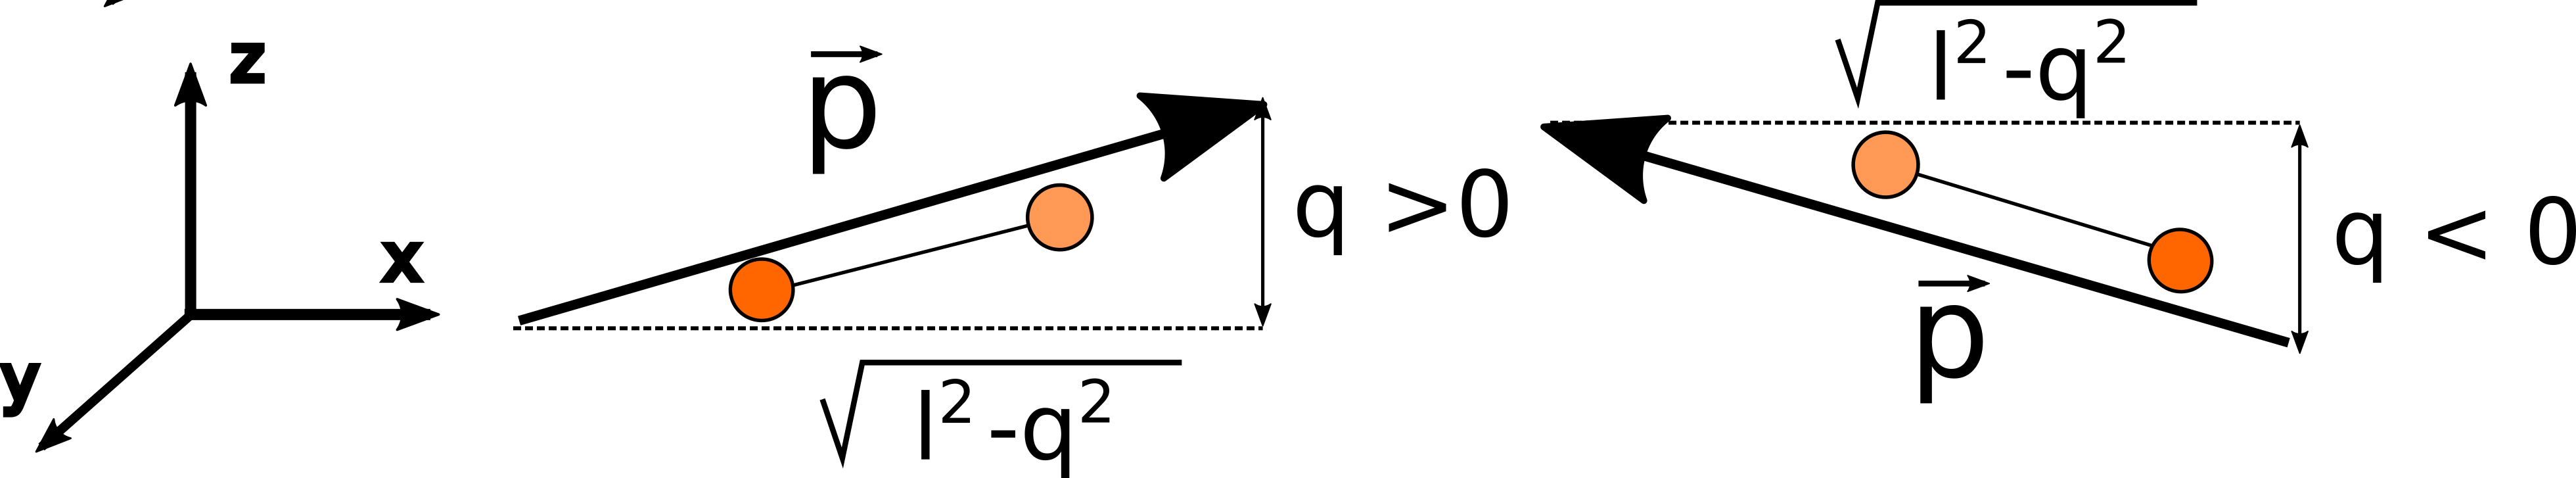
\includegraphics[width=0.8\linewidth]{graphics/DimerQParameterization.png}
		\caption{Parameterization of the dipole moment via z coordinate of right dimer}
		\label{DipoleQParameterization}
	\end{figure}
	The dipole moment can then be written as:
	\begin{equation}
		\vec{p} =	Q\left( \begin{array}{c}
			\sqrt{l^2 -  q^2} \\
			0 \\
			q
		\end{array} \right) \quad \text{for} \quad q > 0 \qquad \text{and} \qquad \vec{p} =  Q	\left(\begin{array}{c}
			\sqrt{l^2 -  q^2} \\
			0 \\
			-q
		\end{array} \right) \quad \text{for} \quad q < 0
	\end{equation}
	We have to confine $q \in \left[-l, l\right]$ then. With this parameterization we could use the usual double well potential. For the interaction, one would probably write down the interaction energy of one dipole in the field of another and then derive for $q$:
	\begin{align}
		\dot{q} &=	p \\
		\dot{p} &=	- \frac{\partial}{\partial q} \left( E(\vec{p}_1(q), \vec{p}_2, \vec{r}) \right) + ...
	\end{align}
	\subsubsection{XY-Model Interaction}[htp]
	We consider a System Hamiltonian of the Form:
	\begin{equation}
		H =	 - \sum_{\left \langle i, j \right \rangle}^{} J \cos \left(\vartheta_i - \vartheta_j \right)  + \sum_i h \cos \left(p	\vartheta_j\right)
	\end{equation}
	The $h$ is associated with a \textbf{symmetry breaking} field. The Pointer angles are confined to $\vartheta \in \left[0, 2\pi \right]$. The $SO(2)$-symmetry is broken through the perturbation, but the $\mathbb{Z}_2$-Symmetry should still be intact (in form of a pointer flip ''$ +\pi$''). The model for $p=2$ has two equilibrium states at $\vartheta =	\frac{\pi}{2}, \frac{3 \pi}{2}$ and is therefore similar to the Ising model. Indeed in \cite{jose1977renormalization} it was shown that a renormalization group approach shows that the model does a second order phase transition with exponents corresponding to a \textbf{p-state planar model} (hopefully it means p-state Potts model?), see \autoref{PhaseXY}.
	
	\begin{figure}
		\centering
		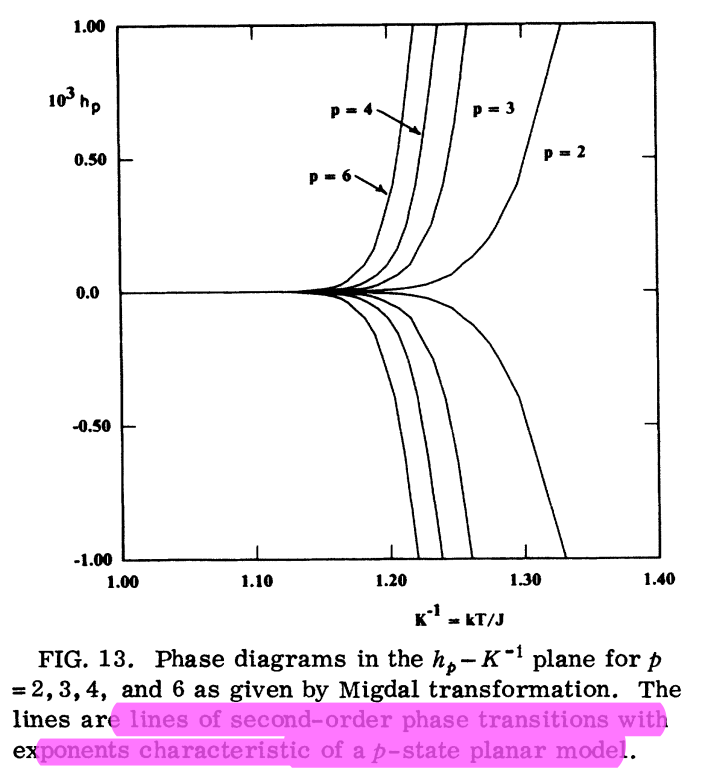
\includegraphics[width=0.8\linewidth]{graphics/Phase-Diagram-XY.png}
		\caption{Phase diagram of symmetry broken XY-model}
		\label{PhaseXY}
	\end{figure}
	\subsection{Quantum Description}
	We will try to describe our model as a two state system, each state living in a displaced harmonic oscillator. The hamiltonian of one lattice site then would be
	\begin{equation}
		H_S =	P_0 \varepsilon_0 + P_1 \varepsilon_1 + \lambda (P_0 - P_1) \otimes (a^\dagger  + a) + \Omega a^\dagger a
	\end{equation}
	This hamiltonian is not diagonal in the eigen-energy basis of the harmonic oscillator which would make the transition to interaction picture difficult. Thats why we introduce the polaron transformation:
	\begin{equation}
		U_p =	e^{\frac{\lambda}{\Omega} (P_0 - P_1) \otimes (a^\dagger - a)}
	\end{equation}
	To transform $H_S$ into the polaron picture, we need to know how the polaron transformation acts on $a^{(\dagger)}$:
	\begin{align}
		U_p a &=	\sum_{k=0}^{\infty} \frac{\left(\frac{\lambda}{\Omega} (P_0 - P_1)\right)^k }{k!} \otimes (a^{\dagger} - a)^k a \\
		&=	\sum_{k=0}^{\infty} \frac{\left(\frac{\lambda}{\Omega} (P_0 - P_1)\right)^k }{k!} \otimes \left(a(a^{\dagger} - a)^k - k (a^\dagger - a)^{k-1}\right) \\
		&= a U_p -  \left(\frac{\lambda}{\Omega} (P_0 - P_1)\right)  \sum_{k}^{} \frac{\left(\frac{\lambda}{\Omega} (P_0 - P_1)\right)^{k -1} \not k (a^\dagger - a)^{k-1} }{ \not k (k-1)!} \\
		&= a U_p - \left(\frac{\lambda}{\Omega} (P_0 - P_1)\right) U_p
	\end{align}
	Implying that
	\begin{equation}
		a_p =	U_p a U_p^\dagger = a  - \left(\frac{\lambda}{\Omega} (P_0 - P_1)\right) \quad \text{and} \quad a_p^\dagger =	a^\dagger  - \left(\frac{\lambda}{\Omega} (P_0 - P_1)\right)
	\end{equation}
	The projectors transform trivially since they commute with every operator in the polaron transformation.
	For the transformed Hamiltonian we then get
	\begin{alignat*}{2}
		H_S^P &=	U_P H_S U_P^\dagger =	&& P_0\varepsilon_0 + P_1 \varepsilon_1 + \lambda (P_0 - P_1) \otimes (U_p a^\dagger U_p^\dagger  +U_p a U_p^\dagger) + \Omega U_p a^\dagger U_p^\dagger U_p a U_p^\dagger \\
		& =	P_0 \varepsilon_0 + P_1 \varepsilon_1 && + \lambda (P_0 - P_1) \otimes \left(	a  - \left(\frac{\lambda}{\Omega} (P_0 - P_1)\right) + 	a^\dagger  - \left(\frac{\lambda}{\Omega} (P_0 - P_1)\right) \right) \\
		& &&+ \Omega \left(a^\dagger  - \left(\frac{\lambda}{\Omega} (P_0 - P_1)\right)\right)\left(a  - \left(\frac{\lambda}{\Omega} (P_0 - P_1)\right)\right) \\
		&=P_0 \varepsilon_0 + P_1 \varepsilon_1 && + \lambda (P_0 - P_1) \otimes (a^\dagger  + a) -\frac{\lambda^2}{\Omega} - \frac{\lambda^2}{\Omega} \\
		& &&+\Omega a^\dagger a - \Omega \frac{\lambda}{\Omega} (P_0 - P_1) \otimes (a^\dagger +a) + \Omega \frac{\lambda^2}{\Omega^2} \\
		&= P_0 \varepsilon_0 + P_1 \varepsilon_1 && -\frac{\lambda^2}{\Omega} + \Omega a^\dagger a
	\end{alignat*}
	\subsubsection{Interaction with state transition}
	If we want to describe a transition from one well to another of the double well potential, we need to model transitions from state $|0\rangle$ to $|1\rangle$ (and the other way around), which means we need to consider jump operators like
	\begin{equation}
		\sigma^- =	|0\rangle \langle 1| \qquad \text{and} \qquad \sigma^+ =	(\sigma^-)^\dagger =	|1\rangle\langle 0 |
	\end{equation}
	with (BCH)
	\begin{alignat*}{2}
		U_p \sigma^- U_p^\dagger &=	\sigma^- &&+ \left[\frac{\lambda}{\Omega} (P_0 - P_1) \otimes (a^\dagger - a), \sigma^-\right] \\
		& &&+	\frac{1}{2!} \left[\frac{\lambda}{\Omega} (P_0 - P_1) \otimes (a^\dagger - a) , \left[\frac{\lambda}{\Omega} (P_0 - P_1) \otimes (a^\dagger - a), \sigma^-\right]\right] \\
		& &&+ ...  \\
		&= \sigma^- &&+ \sigma^- \frac{2 \lambda}{\Omega} (a^\dagger - a) + \sigma^- \frac{1}{2!} \left(\frac{2 \lambda}{\Omega} (a^\dagger - a)\right)^2 + ... \\
		&= \sigma^- && e^{\frac{2\lambda}{\Omega} (a^\dagger -a)} \\
		& =	\sigma_p^{-}
	\end{alignat*}
	The interaction Hamiltonian that we want to look at will be
	\begin{equation}
		H_I^p =	A_I^p \otimes B_I =	(\sigma_p^- + \sigma_p^+) \otimes \sum_k (h_k b_k + h_k^* b_k^\dagger)
	\end{equation}
	Since we want to go into the interaction picture with respect to $H_S^P$ and $H_B =	\sum_k \omega_k b_k^\dagger b_k$, we need to know the time evolution of $\sigma_p^-$:
	\begin{equation}
		\boldsymbol{\sigma}_p^- =	e^{iH_S^pt} \sigma_p^- e^{-iH_S^p t´} =	e^{i (P_0 \varepsilon_0 + P_1 \varepsilon_1)t} \sigma^- e^{-i (P_0 \varepsilon_0 + P_1 \varepsilon_1)t} e^{i (\Omega a^\dagger a)t}e^{\frac{2\lambda}{\Omega} (a^\dagger -a)}  e^{-i (\Omega a^\dagger a)t}
	\end{equation}
	Since $P_a^k =	P_a$, we can rewrite
	\begin{equation}
		e^{iP_0\epsilon_0t} =	\sum_{k=0} \frac{(i\varepsilon_0 t)^k}{k!} P_0^k =	1 + \sum_{k=1} \frac{(i\varepsilon_0 t)^k}{k!} P_0 =	1 + (e^{i\varepsilon_0 t} - 1) P_0
	\end{equation}
	With that
	\begin{equation}
		e^{i (P_0 \varepsilon_0)t} \sigma^- e^{-i (P_0 \varepsilon_0)t} =		\left[1 + (e^{i\varepsilon_0 t} - 1) P_0\right] \sigma^- 	\left[1 + (e^{-i\varepsilon_0 t} - 1) P_0\right] =	\sigma^- e^{i\varepsilon_0t}
	\end{equation}
	For $e^{i (\Omega a^\dagger a)t}e^{\frac{2\lambda}{\Omega} (a^\dagger -a)}  e^{-i (\Omega a^\dagger a)t}$ we can use that the time evolution is unitary and write
	\begin{equation}
		e^{i (\Omega a^\dagger a)t}e^{\frac{2\lambda}{\Omega} (a^\dagger -a)}  e^{-i (\Omega a^\dagger a)t} =	e^{\frac{2\lambda}{\Omega} e^{i (\Omega a^\dagger a)t} (a^\dagger -a) e^{-i (\Omega a^\dagger a)t}}
	\end{equation}
	Which reduces the problem to calculating $e^{i (\Omega a^\dagger a)t} a^{(\dagger)} e^{-i (\Omega a^\dagger a)t}$. We do that by deriving a differential equation:
	\begin{align}
		\frac{d}{dt} \tilde{a}(t) &=	\frac{d}{dt} \left( e^{i (\Omega a^\dagger a)t} a e^{-i (\Omega a^\dagger a)t} \right) =	e^{i (\Omega a^\dagger a)t} \left[i\Omega a^\dagger a, a\right] e^{-i (\Omega a^\dagger a)t} \\
		&= - i \Omega \tilde{a}(t)
	\end{align}
	Which implies that $\tilde{a}(t) =	C e^{-i\Omega t}$, and with the initial condition that $\tilde{a}(0) = a$ we get
	\begin{equation}
		\tilde{a}(t) = e^{i (\Omega a^\dagger a)t} a e^{-i (\Omega a^\dagger a)t} =	a e^{-i\Omega t}
	\end{equation}
	That gives us in total
	\begin{equation}
		\boldsymbol{\sigma}_p^-(t) =	\sigma^- e^{i(\varepsilon_0 - \varepsilon_1) t}  \otimes e^{\frac{2\lambda}{\Omega} (a^\dagger e^{i \Omega t} -a e^{-i \Omega t})}
	\end{equation}
	so that we can now express $\mathbf{A}_I^p (t) =			\boldsymbol{\sigma}_p^-(t) + 		\boldsymbol{\sigma}_p^+(t)$. For deriving a Lindblad-Equation, we start at the Redfield-II equation that already has the degrees of freedom of the bath traced out:
	\begin{align}
		\dot{\boldsymbol{\rho}}_S^p(t) &=	- \int_{0}^{\infty} \left[\boldsymbol{A}_I^p (t), \boldsymbol{A}_I^p (t - \tau) \boldsymbol{\rho}_S^p(t)\right]C(\tau) d\tau + h.c. \\
		&= - \int_{0}^{\infty} \left[\boldsymbol{\sigma}_p^-(t) + 		\boldsymbol{\sigma}_p^+(t), \boldsymbol{\sigma}_p^-(t - \tau) + 		\boldsymbol{\sigma}_p^+(t - \tau) \boldsymbol{\rho}_S^p(t)\right]C(\tau) d\tau + h.c.
	\end{align}
	If we want to do the secular approximation now, we need to consider the $e^{e^{\pm i \Omega t}}$ factors in  $\boldsymbol{\sigma}_p^\pm(t)$ and one (or the only) way to do this is rewriting $\boldsymbol{\sigma}_p^\pm(t)$ as exponential series:
	\begin{align}
		\boldsymbol{\sigma}_p^-(t) &=	\sum_{k, l}^{}e^{-\frac{2\lambda^2}{\Omega^2}} \frac{\left(\frac{2\lambda}{\Omega}\right)^k \left(-\frac{2\lambda}{\Omega}\right)^l}{k! l!}e^{ik\Omega t} (a^\dagger)^k e^{-il\Omega t} a^l \otimes e^{i(\varepsilon_0 - \varepsilon_1)t} \sigma^- \\
		&= \sum_{k, l}^{}e^{-\frac{2\lambda^2}{\Omega^2}} \frac{\left(\frac{2\lambda}{\Omega}\right)^k \left(-\frac{2\lambda}{\Omega}\right)^l}{k! l!} (a^\dagger)^k a^l \otimes \sigma^-  e^{i(\varepsilon_0 - \varepsilon_1 + (k-l)\Omega )t}
	\end{align}
	If we now look at combinations like $\boldsymbol{\sigma}_p^-(t)\boldsymbol{\sigma}_p^-(t - \tau)$, we see that (for every term)
	\begin{equation}
		\boldsymbol{\sigma}_p^-(t)\boldsymbol{\sigma}_p^-(t- \tau) \propto e^{i (2(\varepsilon_0 - \varepsilon_1) - (k-l) \Omega - (m-n) \Omega) t} \cdot e^{-i ((\varepsilon_0 - \varepsilon_1) + (m-n)\Omega)\tau}
	\end{equation}
	If now $2(\varepsilon_0 - \varepsilon_1)$ is not an integer multiple of $\Omega$, as we will assume in the following,  terms like $\boldsymbol{\sigma}_p^\pm(t)\boldsymbol{\sigma}_p^\pm(t- \tau) \boldsymbol{\rho}_S^p(t)$ or $\boldsymbol{\sigma}_p^\pm(t- \tau)  \boldsymbol{\rho}_S^p(t)\boldsymbol{\sigma}_p^\pm(t)$ will oscillate in $t$ and are thus dropped in secular approximation. Therefore we are only interested in terms like:
	\begin{align*}
		\boldsymbol{\sigma}_p^\pm(t)\boldsymbol{\sigma}_p^\mp(t- \tau) \boldsymbol{\rho}_S^p(t) &=	\sum_{klmn}^{} D_{klmn}^\mp e^{\mp i (\varepsilon_0 - \varepsilon_1) \tau} e^{i (k-l) \Omega t} e^{i (m-n) \Omega (t- \tau)} (a^\dagger)^k a^l (a^\dagger)^m a^n \sigma^+ \sigma^- \boldsymbol{\rho}_S^p(t) \\
		&\propto e^{i (\mp(\varepsilon_0 - \varepsilon_1) - (m-n)\Omega) \tau} \cdot e^{i (k-l +m - n)t}
	\end{align*}
	\begin{align*}
		\boldsymbol{\sigma}_p^\pm(t- \tau) \boldsymbol{\rho}_S^p(t)\boldsymbol{\sigma}_p^\mp(t)  &=	\sum_{klmn}^{} D_{klmn}^\mp e^{\pm i (\varepsilon_0 - \varepsilon_1) \tau} e^{i (k-l) \Omega (t - \tau)} e^{i (m-n) \Omega t} \sigma^- (a^\dagger)^k a^l \boldsymbol{\rho}_S^p(t) (a^\dagger)^m a^n  \sigma^+ \\
		&\propto e^{i (\pm(\varepsilon_0 - \varepsilon_1) - (k-l)\Omega) \tau} \cdot e^{i (k-l +m - n)t}
	\end{align*}
	The last exponential factor oscillating in t yields in secular approximation a delta distribution of the form $\delta_{k-l, n-m}$.\\
	The property of the prefactor
	\begin{equation}
		D_{klmn}^+ =	e^{\frac{4\lambda^2}{\Omega^2}} \frac{\left(\frac{2\lambda}{\Omega}\right)^{k + n} \left(-\frac{2\lambda}{\Omega}\right)^{l + m}}{k! l! m! n!} =	D_{mnkl}^-
	\end{equation}
	lets us combine the terms $\boldsymbol{\sigma}_p^\pm(t)\boldsymbol{\sigma}_p^\mp(t- \tau) \boldsymbol{\rho}_S^p(t) + \boldsymbol{\sigma}_p^\mp(t- \tau) \boldsymbol{\rho}_S^p(t)\boldsymbol{\sigma}_p^\pm(t)$ to
	\begin{align*}
		\dot{\boldsymbol{\rho}}_S^p(t) =	&- \int_{0}^{\infty} \sum_{klmn}^{} D_{klmn}^+ \left[\sigma^- \otimes (a^\dagger)^k a^l, \sigma^+ \otimes (a^\dagger)^m a^n \boldsymbol{\rho}_S^p\right] e^{i((\varepsilon_0 - \varepsilon_1) - (m-n)\Omega) \tau} C(\tau) \delta_{k-l, n-m} d\tau \\
		&- \int_{0}^{\infty} \sum_{klmn}^{} D_{klmn}^- \left[\sigma^+ \otimes (a^\dagger)^k a^l, \sigma^- \otimes (a^\dagger)^m a^n \boldsymbol{\rho}_S^p\right] e^{i((\varepsilon_1 - \varepsilon_0) - (m-n)\Omega) \tau} C(\tau) \delta_{k-l, n-m} d\tau \\
		&+ h.c.
	\end{align*}
	The calculation of the Correlation function $C(\tau)$ will be written down later, if we express it through the spectral coupling density, we can write it as a fourier transform:
	\begin{equation}
		C(\tau) =	\frac{1}{2 \pi} \int_{-\infty}^{\infty} \gamma(\omega) e^{-i \omega \tau}d\omega
	\end{equation}
	Inserted in the equation above (and using $\Delta \varepsilon =	\varepsilon_0 - \varepsilon_1$)
	\begin{align*}
		\dot{\boldsymbol{\rho}}_S^p(t) =	&- \int_{-\infty}^{\infty}\int_{0}^{\infty} \sum_{klmn}^{} D_{klmn}^+ \left[..,..\right] e^{-i(\omega - \Delta \varepsilon + (m-n)\Omega) \tau} \frac{1}{2\pi}\gamma(\omega) \delta_{k-l, n-m} d\tau d\omega \\
		&- \int_{-\infty}^{\infty} \int_{0}^{\infty} \sum_{klmn}^{} D_{klmn}^- \left[.., ..\right] e^{-i(\omega + \Delta \varepsilon + (m-n)\Omega) \tau} \frac{1}{2\pi}\gamma(\omega) \delta_{k-l, n-m} d\tau d\omega \\
		&+ h.c.
	\end{align*}
	We can now use the \textbf{Sokhotskij-Plemelj theorem} to perform the $\int d\tau$- integration, leading to
	\begin{align*}
		\dot{\boldsymbol{\rho}}_S^p(t) = -& \int_{-\infty}^{\infty} \sum_{klmn}^{} D_{klmn}^+ \left[...\right] \gamma(\omega) \left(\frac{1}{2} \delta(\omega - (\Delta \varepsilon - (m-n) \Omega)) - \frac{i}{2\pi} \mathcal{P} \frac{1}{\omega - \Delta \varepsilon + (m-n) \Omega}\right) \delta_{k-l, n-m} d\omega  \\
		-& \int_{-\infty}^{\infty} \sum_{klmn}^{} D_{klmn}^- \left[...\right] \gamma(\omega) \left(\frac{1}{2} \delta(\omega + (\Delta \varepsilon + (m-n) \Omega)) - \frac{i}{2\pi} \mathcal{P} \frac{1}{\omega + \Delta \varepsilon + (m-n) \Omega}\right) \delta_{k-l, n-m} d\omega d\omega \\
		&+ h.c.
	\end{align*}
	The second term in the integrals results in the lambs shift which is small and which will be neglected in the following.
	We can use the $\delta$-Distribution to perform the $\int d\omega$-integration, leading to our, for now, final result:
	\begin{align*}
		\dot{\boldsymbol{\rho}}_S^p(t) = &- \frac{1}{2} \sum_{klmn}^{}  D_{klmn}^+ \gamma(\Delta \varepsilon - (m-n) \Omega) \left\{ \left[\sigma^- \otimes (a^\dagger)^k a^l, \sigma^+ \otimes (a^\dagger)^m a^n \boldsymbol{\rho}_S^p\right] + h.c. \right\} \delta_{k-l, n-m} \\
		&-\frac{1}{2} \sum_{klmn}^{}  D_{klmn}^- \gamma(- \Delta \varepsilon - (m-n) \Omega) \left\{ \left[\sigma^+ \otimes (a^\dagger)^k a^l, \sigma^- \otimes (a^\dagger)^m a^n \boldsymbol{\rho}_S^p\right] + h.c. \right\} \delta_{k-l, n-m}
	\end{align*}
	This is still not in Lindblad form and sadly also won't be since we have different powers of creation and annihilation operators in the commutator. We could transform back to the Schrödinger picture now via
	\begin{equation}
		\dot{{\rho}}_S^p(t) =	-i \left[H_S^p, {\rho}_S^p(t)\right] + e^{-i H_S^p t} \dot{\boldsymbol{\rho}}_S^p (t) e^{i H_S^p t}
	\end{equation}
	The $\delta_{k-l, n-m}$ factor ensures that the $e^{i\Omega t}$-Terms that arise when we transform the $a^{(\dagger)}$ compensate so that we just get for the (not yet) Lindblad equation
	\begin{align*}
		\dot{\rho}_S^p(t) = &-i \left[H_S^p,  {\rho}_S^p(t)\right] \\
		&- \frac{1}{2} \sum_{klmn}^{}  D_{klmn}^+ \gamma(\Delta \varepsilon - (m-n) \Omega) \left\{ \left[\sigma^- \otimes (a^\dagger)^k a^l, \sigma^+ \otimes (a^\dagger)^m a^n {\rho}_S^p\right] + h.c. \right\} \delta_{k-l, n-m} \\
		&-\frac{1}{2} \sum_{klmn}^{}  D_{klmn}^- \gamma(- \Delta \varepsilon - (m-n) \Omega) \left\{ \left[\sigma^+ \otimes (a^\dagger)^k a^l, \sigma^- \otimes (a^\dagger)^m a^n {\rho}_S^p\right] + h.c. \right\} \delta_{k-l, n-m}
	\end{align*}
	From here i don't now how to calculate expectation values because of the powers of the creation and annihilation operators. But i tried anyway for the seemingly easiest case $\frac{d}{dt} {\langle \sigma^- \rangle}$:
	It seemed easier to transform back to the ''normal'' picture, since otherwise we would have had to calculate $[\sigma_p^\pm, (a^{(\dagger)})^k]$. Doing the transformation yields:
	\begin{align*}
		\dot{\rho}_S(t) &=	U_p^\dagger \dot{\rho}_S^p(t) U_p \\
		=&-i \left[H_S,  {\rho}_S(t)\right] \\
		&- \frac{1}{2} \sum_{klmn}^{}  D_{klmn}^+ \gamma(\Delta \varepsilon - (m-n) \Omega) \left\{ \left[\sigma^-_{-p} \otimes (a^\dagger_{-p})^k a^l_{-p}, \sigma^+_{-p} \otimes (a^\dagger_{-p})^m a^n_{-p} {\rho}_S\right] + h.c. \right\} \delta_{k-l, n-m} \\
		&-\frac{1}{2} \sum_{klmn}^{}  D_{klmn}^- \gamma(- \Delta \varepsilon - (m-n) \Omega) \left\{ \left[\sigma^+_{-p} \otimes (a^\dagger_{-p})^k a^l_{-p}, \sigma^-_{-p} \otimes (a^\dagger_{-p})^m a^n_{-p} {\rho}_S\right] + h.c. \right\} \delta_{k-l, n-m}
	\end{align*}
	With $_{-p}$ denoting the polaron transformation with $\lambda' =	-\lambda $ yielding
	\begin{equation}
		\sigma^\pm_{-p} =	\sigma^\pm e^{\pm \frac{2\lambda}{\Omega} (a^\dagger -a)} \qquad \text{and} \qquad a^{(\dagger)}_{-p} =	a^{(\dagger)} + \frac{\lambda}{\Omega}(P_0 - P_1)
	\end{equation}
	The commutator of $[(a^{(\dagger)}_{-p})^k, \sigma^-]$ is zero:
	\begin{align*}
		(a^{(\dagger)}_{-p})^k \sigma^- &=	(a^{(\dagger)} + \frac{\lambda}{\Omega}(P_0 - P_1))^k \sigma^- =	\sum_i \binom{k}{i} (a^{(\dagger)})^{k-i} \left(\frac{\lambda}{\Omega}\right)^i (P_0 - P_1)^i \sigma^- \\
		&= \sum_i \binom{k}{i} (a^{(\dagger)})^{k-i} \left(\frac{\lambda}{\Omega}\right)^i \begin{cases}
			\mathbf{1} \sigma^- &\quad \text{i even} \\
			(P_0 - P_1) \sigma^- &\quad \text{i uneven}
		\end{cases} \\
		&= \sigma^- \sum_i \binom{k}{i} (a^{(\dagger)})^{k-i} \left(\frac{\lambda}{\Omega}\right)^i (P_0 - P_1)^i =	\sigma^- (a^{(\dagger)}_{-p})^k
	\end{align*}
	Now we are ready to ''compute''	$\frac{d}{dt} {\langle \sigma^- \rangle}$ via $ \frac{d}{dt} {\langle \sigma^- \rangle} =	\text{tr}\left\{\sigma^- \dot{\rho}_S\right\}$. We split the calculation into three terms, each representing one line of the equation for $\dot{\rho}_S$:
	\begin{alignat*}{2}
		(1) &=	&&-i~ \text{tr}\left\{\sigma^- \left[H_S, \rho_S\right]\right\} \\
		&=	&&-i~ \text{tr} \left\{ \sigma^- P_0 \varepsilon_0 \rho_S + \sigma^- P_1 \varepsilon_1 \rho_S + \lambda (P_0 - P_1) \otimes (a^\dagger + a) \rho_S +\sigma^- \Omega a^\dagger a \rho_S \right\} \\
		& &&- i~ \text{tr} \left\{ \sigma^- \rho_S \varepsilon_0 P_0 - \sigma^- \rho_S \varepsilon_1 P_1 - \sigma^- \rho_S \lambda (P_0 - P_1) \otimes (a^\dagger +a) - \sigma^- \rho_S \Omega a^\dagger a\right\} \\
		&= && - i ~\text{tr} \left\{(\varepsilon_1 - \varepsilon_0)\sigma^- \rho_S - 2 \lambda \sigma^- \otimes (a^\dagger + a) \rho_S\right\} \\
		&= && ~i \Delta \varepsilon \langle \sigma^- \rangle + 2 i \lambda \langle \sigma^- \rangle \sqrt{2 \Omega} \langle x \rangle
	\end{alignat*}
	Here i already am suspicious that this differential equation is complex?
	The next terms only become worse:
	\begin{alignat*}{2}
		(2) =	&- \frac{1}{2} \sum_{klmn}^{}  D_{klmn}^+ \gamma(...) \text{tr}\left\{ \sigma^- \left[\sigma^-_{-p} \otimes (a^\dagger_{-p})^k a^l_{-p}, \sigma^+_{-p} \otimes (a^\dagger_{-p})^m a^n_{-p} {\rho}_S\right] \right\} \delta_{k-l, n-m} \\
		&- \frac{1}{2} \sum_{klmn}^{}  D_{klmn}^+ \gamma(...) \text{tr}\left\{ \sigma^- \left[\rho_S \sigma^-_{-p} \otimes (a^\dagger_{-p})^n a_{-p}^m, \sigma_{-p}^+ \otimes (a^\dagger_{-p})^l a_{-p}^k\right]\right\} \delta_{k-l, n-m}
	\end{alignat*}
	Since $\sigma^- \sigma^- = 0$ and we can freely swap cyclic and commute, actually only one term survives and we get
	\begin{equation}
		(2) =- \frac{1}{2} \sum_{klmn}^{}  D_{klmn}^+ \gamma(...) \text{tr} \left\{ \sigma^- e^{-\frac{2\lambda}{\Omega} (a^\dagger -a)}  (a^\dagger_{-p})^n a_{-p}^m  (a^\dagger_{-p})^l a_{-p}^k\right\}
	\end{equation}
	Yeah i don't now what to do after here.
	
	\subsubsection{Getting to diagonal Lindblad-Form}
	Starting from the Master equation in polaron-schrödinger picture, we consider the term
	\begin{equation}
		D_{klmn}^+ \gamma^+_{(m-n)} \left\{ \left[\sigma^- (a^\dagger)^k a^l, \sigma^+ (a^\dagger)^m a^n {\rho}_S^p\right] + \left[{\rho}_S^p \sigma^- (a^\dagger)^n a^m, \sigma^+ (a^\dagger)^l a^k \right] \right\} \delta_{k-l, n-m}
	\end{equation}
	using $\gamma^+_{m-n} =	\gamma(\Delta \varepsilon - (m-n)\Omega)$. We make the replacements $l = m, k =	n$ in the second term, which yields
	\begin{equation*}
		\left\{ \gamma^+_{(m-n)} D_{klmn}^+ \left[\sigma^-  (a^\dagger)^k a^l, \sigma^+ (a^\dagger)^m a^n {\rho}_S^p\right] + \gamma^+_{(l-k)} D_{nmlk}^+ \left[{\rho}_S^p \sigma^-  (a^\dagger)^k a^l, \sigma^+  (a^\dagger)^m a^n \right] \right\} \delta_{k-l, n-m}
	\end{equation*}
	Note that $D_{klmn}^+ =	D_{nmlk}^+ $ and $\gamma^+_{(m-n)} \delta_{k-l, n-m} =\gamma^+_{(l-k)}	\delta_{k-l, n-m}$, so that we get
	\begin{alignat}{2}
		&=\gamma^+_{(m-n)} D_{klmn}^+&&\{\sigma^-  (a^\dagger)^k a^l \sigma^+ (a^\dagger)^m a^n {\rho}_S^p - \sigma^+ (a^\dagger)^m a^n {\rho}_S^p \sigma^-  (a^\dagger)^k a^l \\
		&~&&+{\rho}_S^p \sigma^-  (a^\dagger)^k a^l \sigma^+  (a^\dagger)^m a^n - \sigma^+  (a^\dagger)^m a^n  {\rho}_S^p \sigma^-  (a^\dagger)^k a^l \} \delta_{k-l, n-m} \\
		&=- \gamma^+_{(m-n)} D_{klmn}^+&& \left\{2 \sigma^+ (a^\dagger)^m a^n {\rho}_S^p \sigma^-  (a^\dagger)^k a^l - \left\{\sigma^-\sigma^+  (a^\dagger)^k a^l (a^\dagger)^m a^n,  {\rho}_S^p\right\} \right\}\delta_{k-l, n-m}
	\end{alignat}
	Which looks a bit more Lindblad but still isn't. To get to a Lindblad form we rewrite the sum
	\begin{equation}
		\sum_{klmn} \gamma^+_{(m-n)} D_{klmn}^+ \left\{2 \sigma^+ (a^\dagger)^m a^n {\rho}_S^p \sigma^-  (a^\dagger)^k a^l - \left\{\sigma^-\sigma^+  (a^\dagger)^k a^l (a^\dagger)^m a^n,  {\rho}_S^p\right\} \right\}\delta_{k-l, n-m}
	\end{equation}
	to sum over $q =	l - k$ and $r =	m - n$ (if i am not mistaken $\sum_{k=0,l=0}^{\infty} A^k B^l = \sum_{q=0}^{\infty} \sum_{k=0}^{\infty} A^k B^{k+q} $)
	\textbf{This is obviously horribly wrong and neglects the terms with $k > l$. Skip to next section for the correct result}:
	\begin{align*}
		&= \sum_{q = 0, r=0}^{\infty} \sum_{kn}^{} \gamma^+_{(r)} D_{k, k+q}^+ D_{n, n+r}^+ \left\{2 \sigma^+ (a^\dagger)^{n+r} a^n {\rho}_S^p \sigma^-  (a^\dagger)^k a^{k+q} - \left\{\sigma^-\sigma^+  (a^\dagger)^k a^{k+q} (a^\dagger)^{n+r} a^n,  {\rho}_S^p\right\} \right\}\delta_{r, q} \\
		&= \sum_q \Bigg \{2 \left(\sqrt{\gamma_q^+} \sum_n D_{n, n+q}^+ \sigma^+ (a^\dagger)^{n+q} a^n\right) {\rho}_S^p \left(\sqrt{\gamma_q^+} \sum_k D_{k, k+q}^+ \sigma^- (a^\dagger)^k a^{k+q}\right) \\
		&\qquad- \left\{\left(\sqrt{\gamma_q^+} \sum_k D_{k, k+q}^+ \sigma^- (a^\dagger)^k a^{k+q}\right) \left(\sqrt{\gamma_q^+} \sum_n D_{n, n+q}^+ \sigma^+ (a^\dagger)^{n+q} a^n\right), \rho_S^p\right\}\Bigg \}
	\end{align*}
	With
	\begin{equation}
		D_{k,k+q}^+ =	e^{\frac{2\lambda^2}{\Omega^2}} \frac{\left(\frac{2\lambda}{\Omega}\right)^{k} \left(-\frac{2\lambda}{\Omega}\right)^{k+q}}{k! (k+q)! }
	\end{equation}
	Since we can obviously rename $n \rightarrow k$ and $\left(\sqrt{\gamma_q^+} \sum_k D_{k, k+q}^+ \sigma^+ (a^\dagger)^{k+q} a^k\right)^\dagger =	\left(\sqrt{\gamma_q^+} \sum_k D_{k, k+q}^+ \sigma^- (a^\dagger)^k a^{k+q}\right) $, we have achieved Lindblad form with the jump operator:
	\begin{equation}
		L_q^+ =	\sqrt{\gamma_q^+} \sum_k D_{k, k+q}^+ \sigma^+ (a^\dagger)^{k+q} a^k
	\end{equation}
	For the term with the $\gamma^-_q =	\gamma(-\Delta \varepsilon - q \Omega))$ prefactor we can do the same calculation and arrive at the jump operator
	\begin{equation}
		L_q^- =	\sqrt{\gamma_q^-} \sum_k D_{k, k+q}^- \sigma^- (a^\dagger)^{k+q} a^k
	\end{equation}
	Which lets us write down the Lindblad equation in polaron picture:
	\begin{align*}
		\dot{\rho}_S^p(t) = &-i \left[H_S^p,  {\rho}_S^p(t)\right] \\
		&+\sum_{q}^{}  \left(L_q^+ \rho_S^p \left(L_q^+\right)^\dagger - \frac{1}{2} \left\{\left(L_q^+\right)^\dagger L_q^+, \rho_S^p \right\}\right) \\
		&+\sum_{q}^{}  \left(L_q^- \rho_S^p \left(L_q^-\right)^\dagger - \frac{1}{2} \left\{\left(L_q^-\right)^\dagger L_q^-, \rho_S^p \right\}\right)
	\end{align*}
	To pursue the idea that we can factorize the two-level expectation values and the harmonic-oscillator expectation values, we transform back into the ''normal'' picture to calculate $\frac{d}{dt} \langle \sigma^- \rangle $. We need to know how the jump operators transform:
	\begin{align}
		U_p^\dagger L_q^+ U_p &=	\sqrt{\gamma_q^+} \sum_k D_{k, k+q}^+ \sigma^+_{-p} (a^\dagger_{-p})^{k+q} a_{-p}^k \\
		&= \sqrt{\gamma_q^+} \sum_k D_{k, k+q}^+ \sigma^+ e^{\frac{2\lambda}{\Omega} \left(a^\dagger - a\right)} \left(a^\dagger + \frac{\lambda}{\Omega} \sigma^z\right)^{k+q} \left(a + \frac{\lambda}{\Omega} \sigma^z \right)^k
	\end{align}
	It is straightforward to commute $\sigma^+$ and $a_p$:
	\begin{align}
		\sigma^+ \left(a + \frac{\lambda}{\Omega} \sigma^z \right)^k &=	\sigma^+ \left(a + \frac{\lambda}{\Omega} \sigma^z \right) \left(a + \frac{\lambda}{\Omega} \sigma^z \right)^{k-1} =	\left(a + \frac{\lambda}{\Omega}\right) \sigma^+ \left(a + \frac{\lambda}{\Omega} \sigma^z \right)^{k-1} \\
		& =	\left(a + \frac{\lambda}{\Omega}\right)^k \sigma^+
	\end{align}
	which leads to
	\begin{align}
		U_p^\dagger L_q^+ U_p &=	\sqrt{\gamma_q^+} \sum_k D_{k, k+q}^+ e^{\frac{2\lambda}{\Omega} \left(a^\dagger - a\right)} \left(a^\dagger + \frac{\lambda}{\Omega}\right)^{k+q} \left(a + \frac{\lambda}{\Omega}\right)^k \otimes \sigma^+ \\
		&= \mathcal{L}_q^+ \otimes \sigma^+
	\end{align}
	Defining
	\begin{align}
		\mathcal{L}_q^+  &= \sqrt{\gamma_q^+} \sum_k D_{k, k+q}^+ e^{\frac{2\lambda}{\Omega} \left(a^\dagger - a\right)} \left(a^\dagger + \frac{\lambda}{\Omega}\right)^{k+q} \left(a + \frac{\lambda}{\Omega}\right)^k \qquad \text{and equivalently} \\
		\mathcal{L}_q^- &= U_p^\dagger L_q^- U_p =	\sqrt{\gamma_q^-} \sum_k D_{k, k+q}^- e^{\frac{2\lambda}{\Omega} \left(a^\dagger - a\right)} \left(a^\dagger- \frac{\lambda}{\Omega}\right)^{k+q} \left(a - \frac{\lambda}{\Omega}\right)^k
	\end{align}
	And $\mathcal{L}_q^+$ acting only on the bosonic modes. So in the normal picture the Lindblad equation has the form
	\begin{align}
		\dot{\rho}_S(t) = &-i \left[H_S,  {\rho}_S(t)\right] \\
		&+\sum_{q}^{}  \left(\mathcal{L}_q^+ \otimes \sigma^+ \rho_S \left(\left(\mathcal{L}_q^+\right)^\dagger \otimes \sigma^-\right) - \frac{1}{2} \left\{\left(\left(\mathcal{L}_q^+\right)^\dagger \otimes \sigma^-\right) \mathcal{L}_q^+ \otimes \sigma^+, \rho_S \right\}\right) \\
		&+\sum_{q}^{}  \left(\mathcal{L}_q^- \otimes \sigma^- \rho_S \left(\left(\mathcal{L}_q^-\right)^\dagger \otimes \sigma^+\right) - \frac{1}{2} \left\{\left(\left(\mathcal{L}_q^-\right)^\dagger \otimes \sigma^+\right) \mathcal{L}_q^- \otimes \sigma^-, \rho_S \right\}\right)
	\end{align}
	In this representation it is easy to see that when calculating $\frac{d}{dt} \langle \sigma^- \rangle$, only the already known term coming from $H_S$ and one from every anticommutator each survive:
	\begin{alignat*}{2}
		\frac{d}{dt} \langle \sigma^- \rangle  &=&&+i \Delta \varepsilon \langle \sigma^- \rangle + 2 i \lambda \langle \sigma^- \rangle \sqrt{2 \Omega} \langle x \rangle \\
		~&~&&-\frac{1}{2} \sum_q \text{tr}\left\{\sigma^- \rho_S  \left(\left(\mathcal{L}_q^+\right)^\dagger \otimes \sigma^-\right) \mathcal{L}_q^+ \otimes \sigma^+ \right\} \\
		~&~&&-\frac{1}{2} \sum_q \text{tr}\left\{\sigma^-\left(\left(\mathcal{L}_q^-\right)^\dagger \otimes \sigma^+\right) \mathcal{L}_q^- \otimes \sigma^- \rho_S \right\} \\
		&= &&+i \Delta \varepsilon \langle \sigma^- \rangle + 2 i \lambda \langle \sigma^- \rangle \sqrt{2 \Omega} \langle x \rangle \\
		~&~&&-\frac{1}{2} \sum_q \text{tr}\left\{\sigma^- \otimes \left(\mathcal{L}_q^+\right)^\dagger \mathcal{L}_q^+  \rho_S  \right\} \\
		~&~&&-\frac{1}{2} \sum_q \text{tr}\left\{\sigma^- \otimes \left(\mathcal{L}_q^-\right)^\dagger  \mathcal{L}_q^- \rho_S \right\} \\
		&= +i &&\Delta \varepsilon \langle \sigma^- \rangle + 2 i \lambda \langle \sigma^- \rangle \sqrt{2 \Omega} \langle x \rangle - \frac{1}{2} \sum_q \left(\left\langle \left(\mathcal{L}_q^+\right)^\dagger \mathcal{L}_q^+\right\rangle  + \left\langle \left(\mathcal{L}_q^-\right)^\dagger \mathcal{L}_q^-\right\rangle \right) \langle \sigma^- \rangle
	\end{alignat*}
	Calculating this expectation value for coherent states, which should or might be possible, could result in just a number for the sum and therefore an actual simple equation?
	\subsubsection{Correction to diagonal Lindblad form}
	Using that
	\begin{align*}
		\sum_{k,l,m,n=0}^{\infty} \delta_{k-l, n-m} = ~~~&\sum_{k}^{} \sum_{l > k}^{} \sum_{m}^{} \sum_{n \geq m}^{} \delta_{k-l, n-m} + \sum_{k}^{} \sum_{l \leq k}^{} \sum_{m}^{} \sum_{n \geq m}^{} \delta_{k-l, n-m} \\
		+ &\sum_{k}^{} \sum_{l \leq k}^{} \sum_{m}^{} \sum_{n < m}^{} \delta_{k-l, n-m} + \sum_{k}^{} \sum_{l > k}^{} \sum_{m}^{} \sum_{n < m}^{} \delta_{k-l, n-m} \\
		=~~~&\sum_{k}^{} \sum_{l \leq k}^{} \sum_{m}^{} \sum_{n \geq m}^{} \delta_{k-l, n-m} + \sum_{k}^{} \sum_{l > k}^{} \sum_{m}^{} \sum_{n < m}^{} \delta_{k-l, n-m} \\
	\end{align*}
	(The first and third term are zero since the condition of the $\delta$ cannot be fulfilled), one can obtain an expression for
	\begin{align*}
		\sum_{klmn}^{} A^m B^n A^k A^l \delta_{k-l, n-m} =	&~~~\sum_{mk}^{} A^m B^m A^k B^k \\
		&+\sum_{q=1}^{\infty}\sum_{mk}^{} A^m B^{m+q} A^{k+q} B^k \\
		&+\sum_{q=1}^{\infty}\sum_{mk}^{} A^{m+q}  B^{m} A^k B^{k+q}
	\end{align*}
	Those relations applied to the Polaron master equation lead to
	\begin{align*}
		\dot{\rho}_S^p(t) = &-i \left[H_S^p,  {\rho}_S^p(t)\right] \\
		&+\sum_{q=1}^{}  \left(L_q^{+-} \rho_S^p \left(L_q^{+-}\right)^\dagger - \frac{1}{2} \left\{\left(L_q^{+-}\right)^\dagger L_q^{+-}, \rho_S^p \right\}\right) \\
		&+\sum_{q=0}^{}  \left(L_q^{++} \rho_S^p \left(L_q^{++}\right)^\dagger - \frac{1}{2} \left\{\left(L_q^{++}\right)^\dagger L_q^{++}, \rho_S^p \right\}\right) \\
		&+\sum_{q=1}^{}  \left(L_q^{-+} \rho_S^p \left(L_q^{-+}\right)^\dagger - \frac{1}{2} \left\{\left(L_q^{-+}\right)^\dagger L_q^{-+}, \rho_S^p \right\}\right) \\
		&+\sum_{q=0}^{}  \left(L_q^{--} \rho_S^p \left(L_q^{--}\right)^\dagger - \frac{1}{2} \left\{\left(L_q^{--}\right)^\dagger L_q^{--}, \rho_S^p \right\}\right) \\
	\end{align*}
	With
	\begin{equation*}
		L_q^{+-} =	\sqrt{\gamma_{-q}^+} \sum_k D_{k + q,k}^+ \sigma^+ (a^\dagger)^{k} a^{k+q} \qquad L_q^{++} =	\sqrt{\gamma_{q}^+} \sum_k D_{k,k+q}^+ \sigma^+ (a^\dagger)^{k+q} a^{k}
	\end{equation*}
	\begin{equation*}
		L_q^{-+} =	\sqrt{\gamma_{q}^-} \sum_k D_{k,k+q}^- \sigma^- (a^\dagger)^{k+q} a^{k} \qquad L_q^{--} =	\sqrt{\gamma_{-q}^-} \sum_k D_{k+q,k}^- \sigma^- (a^\dagger)^{k} a^{k+q}
	\end{equation*}
	A nicer way to write this down would be
	\begin{align*}
		\dot{\rho}_S^p(t) = &-i \left[H_S^p,  {\rho}_S^p(t)\right] \\
		&+\sum_a  \left(L^{aa} \rho_S^p \left(L^{aa}\right)^\dagger - \frac{1}{2} \left\{\left(L^{aa}\right)^\dagger L^{aa}, \rho_S^p \right\}\right)  \qquad \quad \left(L^{aa} =	L_0^{aa}\right) \\
		&+\sum_{ab} \sum_{q=1}^{}  \left(L_q^{ab} \rho_S^p \left(L_q^{ab}\right)^\dagger - \frac{1}{2} \left\{\left(L_q^{ab}\right)^\dagger L_q^{ab}, \rho_S^p \right\}\right) \\
	\end{align*}
	\subsubsection{Expanding in $\lambda$}
	To \textbf{0th order} only the terms with $q=0$ and $k=0$ survive, e.g. the first term of the $L^{aa}-$operators, which results in
	\begin{align*}
		\dot{\rho}_S^p(t) = &-i \left[H_S^p,  {\rho}_S^p(t)\right] \\
		&+\gamma_0^+ \left( \sigma^+ \rho_S^p \sigma^- - \frac{1}{2} \left\{\sigma^- \sigma^+, \rho_S^p \right\}\right) + \gamma_0^- \left(  \sigma^- \rho_S^p \sigma^+ - \frac{1}{2} \left\{\sigma^+ \sigma^-, \rho_S^p \right\}\right)
	\end{align*}
	To \textbf{first order} in $\lambda$: There are no first order terms since the $k=1$-Term of $L^{aa}$ is already second order in $\lambda$, as well as the $q=1$ terms of combinations $L_q^{ab}(L_q^{ab})^\dagger$. So we advance to \textbf{second order}: We now have to take into account the $k=1$-Terms of the $L^{aa}$ and the $q = 1, k,l =	0$-Terms of the $L^{ab}_q$. The former yields an additional $-\frac{4\lambda^2}{\Omega^2} a^\dagger a$ to the $\sigma^\pm$:
	\begin{align*}
		&\gamma_0^+ \left( \sigma^+\left(1 - \frac{4 \lambda^2}{\Omega^2} a^\dagger a\right)\rho_S^p \sigma^- \left(1 - \frac{4 \lambda^2}{\Omega^2} a^\dagger a\right) - \frac{1}{2} \left\{\sigma^-\left(1 - \frac{4 \lambda^2}{\Omega^2} a^\dagger a\right) \sigma^+ \left(1 - \frac{4 \lambda^2}{\Omega^2} a^\dagger a\right), \rho_S^p \right\}\right)
	\end{align*}
	For the $L^{ab}_q$-Terms we get terms like
	\begin{align*}
		L_1^{+-} \rho_S^p \left(L_1^{+-}\right)^\dagger - \frac{1}{2} \left\{\left(L_1^{+-}\right)^\dagger L_1^{+-}, \rho_S^p \right\} =	\frac{4 \lambda^2}{\Omega^2} \gamma_{-1}^+ \left(a \otimes \sigma^+ \rho_S^P a^\dagger \otimes \sigma^-  - \frac{1}{2} \left\{a^\dagger a \otimes P_0, \rho_S^p\right\}\right)
	\end{align*}
	Following this scheme, we arrive at the 2nd order approximation
	\begin{align*}
		\dot{\rho}_S^p(t) = &-i \left[H_S^p,  {\rho}_S^p(t)\right] \\
		&+\gamma_0^+ \left( \sigma^+ \rho_S^p \sigma^- - \frac{1}{2} \left\{\sigma^- \sigma^+, \rho_S^p \right\}\right) + \gamma_0^- \left(  \sigma^- \rho_S^p \sigma^+ - \frac{1}{2} \left\{\sigma^+ \sigma^-, \rho_S^p \right\}\right) \\
		&- \frac{4 \lambda^2}{\Omega^2} \gamma^+_0 \left(\sigma^+ \otimes a^\dagger a \rho_S^p \sigma^- + \frac{1}{2} \left\{\sigma^- \sigma^+ \otimes a^\dagger a, \rho_S^p \right\}\right) \\
		&- \frac{4 \lambda^2}{\Omega^2} \gamma^+_0 \left(\sigma^+ \rho_S^p \sigma^- \otimes a^\dagger a  + \frac{1}{2} \left\{\sigma^- \sigma^+ \otimes a^\dagger a, \rho_S^p \right\}\right) \\
		&- \frac{4 \lambda^2}{\Omega^2} \gamma^-_0 \left(\sigma^- \otimes a^\dagger a \rho_S^p \sigma^+ + \frac{1}{2} \left\{\sigma^+ \sigma^- \otimes a^\dagger a, \rho_S^p \right\}\right) \\
		&- \frac{4 \lambda^2}{\Omega^2} \gamma^-_0 \left(\sigma^- \rho_S^p \sigma^+ \otimes a^\dagger a  + \frac{1}{2} \left\{\sigma^+ \sigma^- \otimes a^\dagger a, \rho_S^p \right\}\right) \\
		&+ \frac{4 \lambda^2}{\Omega^2} \gamma^+_{1} \left(a^\dagger \otimes \sigma^+ \rho_S^p a \otimes \sigma^- - \frac{1}{2}\left\{aa^\dagger \otimes P_0, \rho_S^p \right\}\right) \\
		&+ \frac{4 \lambda^2}{\Omega^2} \gamma^+_{-1} \left(a\otimes \sigma^+ \rho_S^p a^\dagger  \otimes \sigma^- - \frac{1}{2}\left\{a^\dagger a\otimes P_0, \rho_S^p \right\}\right) \\
		&+ \frac{4 \lambda^2}{\Omega^2} \gamma^-_{1} \left(a^\dagger \otimes \sigma^- \rho_S^p a \otimes \sigma^+ - \frac{1}{2}\left\{aa^\dagger \otimes P_1, \rho_S^p \right\}\right) \\
		&+ \frac{4 \lambda^2}{\Omega^2} \gamma^-_{-1} \left(a\otimes \sigma^- \rho_S^p a^\dagger  \otimes \sigma^+ - \frac{1}{2}\left\{a^\dagger  a\otimes P_1, \rho_S^p \right\}\right) \\
	\end{align*}
	\subsubsection{Rate Equation}
	For the rate equation, which describes the rate at which states transform into each other, we need to calculate terms like
	\begin{equation}
		\gamma_{ab,ab} =	\delta_{E_b - E_a, E_b - E_a} \gamma \left(E_b - E_a \right) \langle a | A | b \rangle \langle a | A^\dagger | b \rangle
	\end{equation}
	The states $|a / b\rangle$ are energy eigenstates and are in polaron picture states like
	\begin{equation}
		|a\rangle =	|s\rangle \otimes |n\rangle \qquad \text{with} \qquad s \in \{0, 1\}, \quad n \in \mathbb{N}
	\end{equation}
	In polaron picture $A \equiv A_p =	\sigma^+ \otimes e^{- \frac{2 \lambda}{\Omega} (a^\dagger -a)} + \sigma^- \otimes e^{\frac{2 \lambda}{\Omega} (a^\dagger -a)} $, so that
	\begin{align*}
		\langle a | A | b \rangle &=	\left(\langle s | \otimes \langle n | \right) \left(\sigma^+ \otimes e^{- \frac{2 \lambda}{\Omega} (a^\dagger -a)} + \sigma^- \otimes e^{\frac{2 \lambda}{\Omega} (a^\dagger -a)}\right) (|s'\rangle \otimes |n'\rangle) \\
		&= \langle s | \sigma^+ | s' \rangle \langle n | e^{- \frac{2 \lambda}{\Omega} (a^\dagger -a)} | n' \rangle + \langle s | \sigma^- | s' \rangle \langle n | e^{ \frac{2 \lambda}{\Omega} (a^\dagger -a)} | n' \rangle
	\end{align*}
	The $\langle s | \sigma^\pm | s' \rangle$ are easy to evaluate
	\begin{equation}
		\langle s | \sigma^+ | s' \rangle =	\delta_{s, 1} \delta_{s', 0} \qquad \qquad  \langle s | \sigma^- | s' \rangle =	\delta_{s, 0} \delta_{s', 1}
	\end{equation}
	The $\langle n | e^{ \frac{2 \lambda}{\Omega} (a^\dagger -a)} | n' \rangle$ on the other hand...
	We can use BCH again:
	\begin{align}
		\langle n | e^{ -\frac{2 \lambda}{\Omega} (a^\dagger -a)} | n' \rangle &=	e^{-\frac{2\lambda^2}{\Omega^2}} \sum_{kl} \frac{\left(-\frac{2\lambda}{\Omega}\right)^k \left(\frac{2 \lambda}{\Omega} \right)^l}{k! l!} \langle n | \left(a^\dagger\right)^k a^l | n' \rangle \\
		&= e^{-\frac{2\lambda^2}{\Omega^2}} \sum_{kl} \frac{\left(-\frac{2\lambda}{\Omega}\right)^k \left(\frac{2 \lambda}{\Omega} \right)^l}{k! l!} \sqrt{\frac{n!}{(n-k)!}} \sqrt{\frac{n'!}{(n'-l)!}} \langle n - k|n'-l \rangle \\
		&= e^{-\frac{2\lambda^2}{\Omega^2}} \sum_{kl} \frac{\left(-\frac{2\lambda}{\Omega}\right)^k \left(\frac{2 \lambda}{\Omega} \right)^l}{k! l!} \sqrt{\frac{n!}{(n-k)!}} \sqrt{\frac{n'!}{(n'-l)!}} \delta_{n-k, n'-l}
	\end{align}
	So we get for
	\begin{align*}
		\langle a | A | b \rangle \langle a | A^\dagger | b\rangle =&	e^{\frac{4\lambda^2}{\Omega^2}} \sum_{klpm} \frac{\left(-\frac{2\lambda}{\Omega}\right)^{k+m} \left(\frac{2 \lambda}{\Omega} \right)^{l+p}}{k!m! l!p!} \frac{n!n'!}{(n-k)! (n'-p!)} \delta_{n-k, n'-l} \delta_{n-m, n'-p} \delta_{s,1} \delta_{s', 0} \\
		+& e^{\frac{4\lambda^2}{\Omega^2}} \sum_{klpm} \frac{\left(\frac{2\lambda}{\Omega}\right)^{k+m} \left(-\frac{2 \lambda}{\Omega} \right)^{l+p}}{k!m! l!p!} \frac{n!n'!}{(n'-k)! (n-p!)} \delta_{n-k, n'-l} \delta_{n-m, n'-p} \delta_{s,0} \delta_{s', 1}
	\end{align*}
	And for $\gamma_{ab, ab}$:
	\begin{equation}
		\gamma_{|s\rangle \otimes |n\rangle, |s' \rangle \otimes |n'\rangle } =	\gamma_{ab} \equiv \gamma_{ab, ab} = (\varepsilon_{s'} - \varepsilon_{s} + (n' -n) \Omega) \langle a | A | b \rangle \langle a | A^\dagger | b\rangle
	\end{equation}
	In the rate equation, one would then sum over
	\begin{align}
		\rho_{ib} \propto \sum_a \gamma_{ab} =&	\sum_{s'=0}^{1} \sum_{n'=0}^{\infty}  	\gamma_{|s'\rangle \otimes |n'\rangle, |s \rangle \otimes |n\rangle } \\
		=& 	e^{\frac{4\lambda^2}{\Omega^2}} \sum_{klpm} \frac{\left(-\frac{2\lambda}{\Omega}\right)^{k+m} \left(\frac{2 \lambda}{\Omega} \right)^{l+p}}{k!m! l!p!} \frac{n!(n + (l-k))!}{(n-k)! ((n + (l-k))-p!)} \delta_{k-l, m-p} \delta_{s, 0} \\
		&+ e^{\frac{4\lambda^2}{\Omega^2}} \sum_{klpm} \frac{\left(\frac{2\lambda}{\Omega}\right)^{k+m} \left(-\frac{2 \lambda}{\Omega} \right)^{l+p}}{k!m! l!p!} \frac{n!(n + (l-k))!}{(n-k)! ((n + (l-k))-p!)} \delta_{k-l, m- p}  \delta_{s,1}
	\end{align}
	\subsubsection{Interaction with only creation and annihilation operator}
	Looking at the Interaction (B as before)
	\begin{equation}
		H_I =	(a^\dagger + a) \otimes B_I \qquad \Rightarrow \qquad \boldsymbol{H}_I^P (t) =	(\boldsymbol{a}_p^\dagger + \boldsymbol{a}_p) \otimes \boldsymbol{B}_I
	\end{equation}
	With
	\begin{equation}
		\boldsymbol{a}_p^{(\dagger)} =	e^{iH_S^pt} a_p^{(\dagger)} e^{-iH_S^p t} = a^{(\dagger)} e^{(-) -i \Omega t}	 - \frac{\lambda}{\Omega} (P_0 - P_1)
	\end{equation}
	Which gives us
	\begin{equation}
		\boldsymbol{H}_I^P (t) =	\left(a^{\dagger} e^{i \Omega t}	 + a e^{- i \Omega t} - \frac{2\lambda}{\Omega} (P_0 - P_1) \right) \otimes \boldsymbol{B}_I
	\end{equation}
	Since we use the same bath as before, we can again start at the Redfield-II equation:
	\begin{align*}
		\dot{\boldsymbol{\rho}}_S^p(t) &=	- \int_{0}^{\infty} \left[\boldsymbol{A}_I^p (t), \boldsymbol{A}_I^p (t - \tau) \boldsymbol{\rho}_S^p(t)\right]C(\tau) d\tau + h.c. \\
		&= - \int_{0}^{\infty} \left[\boldsymbol{a}_p^\dagger(t) + 		\boldsymbol{a}_p(t), (\boldsymbol{a}_p^\dagger(t - \tau) + 		\boldsymbol{a}_p(t - \tau)) \boldsymbol{\rho}_S^p(t)\right]C(\tau) d\tau + h.c. \\
		&=	- \int_{0}^{\infty} \left[a^{\dagger} e^{i \Omega t}	 + a e^{- i \Omega t} - \frac{2\lambda}{\Omega} (P_0 - P_1), \left(a^{\dagger} e^{i \Omega (t - \tau)}	 + a e^{- i \Omega (t - \tau)} - \frac{2\lambda}{\Omega} (P_0 - P_1)\right) \boldsymbol{\rho}_S^p(t)\right]C(\tau) d\tau + h.c.
	\end{align*}
	In secular approximation only terms with mixed $a, a^\dagger$ or none at all survive, leaving us with
	\begin{align*}
		\dot{\boldsymbol{\rho}}_S^p(t) =	&- \int_{0}^{\infty} \left\{\left[a^\dagger, a \boldsymbol{\rho}_S^p(t)\right]e^{i \Omega \tau}  + \left[a, a^\dagger \boldsymbol{\rho}_S^p(t) \right]e^{-i \Omega \tau}  + \frac{4\lambda^2}{\Omega^2} \left[(P_0 - P_1), (P_0 - P_1) \boldsymbol{\rho}_S^p(t) \right]\right\} C(\tau) d\tau \\
		&+ h.c.
	\end{align*}
	The first two terms are known from the calculation for the harmonic oscillator, which leaves us to deal with the last term.
	\begin{align*}
		&~- \int_{0}^{\infty} \left\{\frac{4\lambda^2}{\Omega^2} \left[(P_0 - P_1), (P_0 - P_1) \boldsymbol{\rho}_S^p(t) \right]\right\} C(\tau) d\tau + h.c	 \\
		=&- \int_{-\infty}^{\infty}\int_{0}^{\infty} \left\{\frac{4\lambda^2}{\Omega^2} \left[(P_0 - P_1), (P_0 - P_1) \boldsymbol{\rho}_S^p(t) \right]\right\}  \frac{1}{2\pi} \gamma(\omega) e^{-i\omega \tau }d\tau d\omega + h.c \\
		=&-\int_{-\infty}^{\infty} \left\{\frac{4\lambda^2}{\Omega^2} \left[(P_0 - P_1), (P_0 - P_1) \boldsymbol{\rho}_S^p(t) \right]\right\}   \gamma(\omega) \left\{\frac{1}{2} \delta(\omega) - \frac{i}{2 \pi} \mathcal{P} \frac{1}{\omega}\right\} d\omega + h.c \\
		=&- \frac{1}{2} \gamma(0) \frac{4\lambda^2}{\Omega^2} \left\{\left[(P_0 - P_1), (P_0 - P_1) \boldsymbol{\rho}_S^p(t) \right] + \left[  \boldsymbol{\rho}_S^p(t) (P_0 - P_1), (P_0 - P_1) \right] \right\} \\
		~&-\frac{i}{2 \pi} \mathcal{P} \frac{4\lambda^2}{\Omega^2} \int_{-\infty}^{\infty} \frac{\gamma(\omega)}{\omega}  \left\{\left[(P_0 - P_1), (P_0 - P_1) \boldsymbol{\rho}_S^p(t) \right] - \left[  \boldsymbol{\rho}_S^p(t) (P_0 - P_1), (P_0 - P_1) \right] \right\} \\
		=&+\frac{4 \lambda^2}{\Omega^2} \gamma(0) \left[(P_0 - P_1) \boldsymbol{\rho}_S^p(t) (P_0 - P_1) - \boldsymbol{\rho}_S^p(t)\right] \\
		~&-\frac{i}{2 \pi} \mathcal{P} \frac{4\lambda^2}{\Omega^2} \int_{-\infty}^{\infty} \frac{\gamma(\omega)}{\omega} \left[(P_0 - P_1)^2, \boldsymbol{\rho}_S^p(t)\right] \qquad \text{This term is zero since } (P_0 - P_1)^2 =	1
	\end{align*}
	When transforming to the Schrödinger picture, this new term also transforms trivially as the projection operators do not transform at all, which leaves us with
	\begin{align}
		{\rho}_S^p(t) =	&-i \left[\varepsilon_0 P_0 + \varepsilon_1 P_1 + (\Omega + \Delta \Omega) a^\dagger a , {\rho}_S^p(t)\right] \\
		&+ \Gamma(\Omega) \left[1 + n_B(\Omega)\right] \left[a {\rho}_S^p(t) a^\dagger - \frac{1}{2} \left\{a^\dagger a, {\rho}_S^p(t)\right\}\right] \\
		&+\Gamma(\Omega) n_B(\Omega) \left[a^\dagger {\rho}_S^p(t) a- \frac{1}{2} \left\{aa^\dagger , {\rho}_S^p(t)\right\}\right] \\
		&+ \frac{4 \lambda^2}{\Omega^2} \Gamma(0)n_B(0) \left[(P_0 - P_1) {\rho}_S^p(t) (P_0 - P_1) - {\rho}_S^p(t)\right]
	\end{align}
	Now we can derive differential equations for the operator mean values. For a general operator $C$ what actually should be true is
	\begin{align}
		\frac{\text{d}}{\text{d}t} \langle C \rangle &=	\frac{\text{d}}{\text{d}t} \text{tr}\left\{C \rho_S\right\} = \text{tr}\left\{C  \frac{\text{d}}{\text{d}t} \rho_S\right\} =	 \text{tr}\left\{C  \frac{\text{d}}{\text{d}t} (U_p^\dagger \rho_S^p U_p)\right\} =	\text{tr}\left\{ U_p C U_p^\dagger  \frac{\text{d}}{\text{d}t} \rho_S^p \right\} \\
		&=	\text{tr} \left\{C_p \frac{\text{d}}{\text{d}t} \rho_S^p \right\} =	\frac{\text{d}}{\text{d}t} \langle C_p \rangle
	\end{align}
	So it should not matter in which picture we calculate the differential equation. For some reason i get different results, probably a error, but I will present both ways here and hopefully recover the error in the process. \\
	\textbf{Calculation in polaron picture}: \\
	We start by calculating $\frac{\text{d}}{\text{d}t} \langle a_p \rangle$:
	\begin{equation}
		\frac{\text{d}}{\text{d}t} \langle a_p \rangle =	\text{tr} \left\{\left(a - 1 \otimes \frac{\lambda}{\Omega} (P_0 - P_1)\right) \dot{\rho}_S^p\right\} =	\text{tr} \left\{a \dot{\rho}_S^p\right\} - \text{tr} \left\{1 \otimes \frac{\lambda}{\Omega} (P_0 - P_1) \dot{\rho}_S^p\right\}
	\end{equation}
	For a lindblad-equation, if an operator commutes with a certain jump operator $\left[L_k^{(\dagger)}, a\right] =	0$, the trace operation over the corresponding dissipator term will be zero since:
	\begin{align}
		&~\text{tr} \left\{ a \left(L_k \rho_S L_k^\dagger - \frac{1}{2} \left\{L_k^\dagger L, \rho_S \right\}\right) \right\} =	\text{tr} \left\{ a L_k \rho_S L_k^\dagger - \frac{1}{2} a L_k^\dagger L \rho_S - \frac{1}{2} a \rho_S L_k^\dagger L \right\} \\
		=&~ \text{tr} \left\{ a L_k^\dagger L \rho_S - \frac{1}{2} a L_k^\dagger L \rho_S - \frac{1}{2} a L_k^\dagger L \rho_S \right\} = 0
	\end{align}
	The same applies for parts of system hamiltonian that the operator commutes with $ \left[H_S^0, a\right] = 0$ with $H_S =	H_S^0 + H_S^1$ since
	\begin{align*}
		\text{tr} \left\{a \left[H_S^0 + H_S^1, \rho_S\right]\right\} &=	\text{tr} \left\{a \left[H_S^0 , \rho_S\right]\right\} +\text{tr} \left\{a \left[H_S^1, \rho_S\right]\right\} \\
		&=	\text{tr} \left\{a H_S^0 \rho_S - a \rho_S H_S^0 \right\} + \text{tr} \left\{a \left[H_S^1, \rho_S\right]\right\} \\
		&= \text{tr} \left\{a H_S^0 \rho_S - a H_S^0 \rho_S  \right\} + \text{tr} \left\{a \left[H_S^1, \rho_S\right]\right\} =	\text{tr} \left\{a \left[H_S^1, \rho_S\right]\right\}
	\end{align*}
	Which means we only have to look after the not-commuting terms when performing the trace, meaning that $	\text{tr} \left\{a \dot{\rho}_S^p\right\}$ is basically calculated by the exact same steps as in the harmonic oscillator case, but we have to be careful when rewriting the trace as expectation value:
	\begin{align*}
		\text{tr} \left\{a \dot{\rho}_S^p\right\} &=	\left[-i \Omega - \frac{\Gamma(\Omega)}{2}\right] \text{tr}\left\{a \rho_S^p\right\} = \left[-i \Omega - \frac{\Gamma(\Omega)}{2}\right] \text{tr}\left\{\left(a_p + \frac{\lambda}{\Omega} (P_0 - P_1)\right) \rho_S^p\right\} \\
		&= \left[-i \Omega - \frac{\Gamma(\Omega)}{2}\right] \left( \langle a_p \rangle + \frac{\lambda}{\Omega } \langle P_0 - P_1 \rangle\right)
	\end{align*}
	In the second term, $\text{tr} \left\{1 \otimes \frac{\lambda}{\Omega} (P_0 - P_1) \dot{\rho}_S^p\right\}$, the operator commutes with everything, so the trace operation yields just zero leaving us with:
	\begin{equation}
		\frac{\text{d}}{\text{d}t} \langle a_p \rangle = \left[-i \Omega - \frac{\Gamma(\Omega)}{2}\right] \left( \langle a_p \rangle + \frac{\lambda}{\Omega } \langle P_0 - P_1 \rangle\right)
	\end{equation}
	Complex conjugating yields
	\begin{equation}
		\frac{\text{d}}{\text{d}t} \langle a_p^\dagger \rangle = \left[i \Omega - \frac{\Gamma(\Omega)}{2}\right] \left( \langle a_p^\dagger \rangle + \frac{\lambda}{\Omega } \langle P_0 - P_1 \rangle\right)
	\end{equation}
	Which lets us calculate a differential equation for the expectation value of x:
	\begin{align}
		\frac{\text{d}}{\text{d}t} \langle x \rangle &= \frac{\text{d}}{\text{d}t} \left\langle \frac{1}{\sqrt{2 \Omega}}(a_p^\dagger + a_p) \right\rangle =	\frac{1}{\sqrt{2 \Omega}} \left(\frac{\text{d}}{\text{d}t} \langle a_p^\dagger \rangle + \frac{\text{d}}{\text{d}t} \langle a_p \rangle\right) \\
		&= i\sqrt{\frac{\Omega}{2}} \left( \langle a_p^\dagger \rangle - \langle a_p \rangle \right) - \frac{\Gamma(\Omega)}{2 \sqrt{2 \Omega}} \left( \langle a_p^\dagger \rangle + \langle a_p \rangle +  \frac{2 \lambda}{\Omega } \langle P_0 - P_1 \rangle \right) \\
		&= \langle p \rangle - \frac{\Gamma(\Omega)}{2} \left( \langle x \rangle + \frac{2\lambda}{\sqrt{2 \Omega^3} } \langle P_0 - P_1 \rangle\right)
	\end{align}
	Which only differs from the differential equation for the harmonic oscillator from the constant term that depends on whether we are in state 0 or 1. This seems logical considering that we looked at a harmonic potential that was imposed with a linear term that depended on the state.
	
	For the differential equation of $\langle p \rangle$ we get
	\begin{align}
		\frac{\text{d}}{\text{d}t} \langle p \rangle &= \frac{\text{d}}{\text{d}t} \left\langle i\sqrt{\frac{\Omega}{2}}(a_p^\dagger - a_p) \right\rangle =	i\sqrt{\frac{\Omega}{2}} \left(\frac{\text{d}}{\text{d}t} \langle a_p^\dagger \rangle - \frac{\text{d}}{\text{d}t} \langle a_p \rangle\right) \\
		&= i\sqrt{\frac{\Omega}{2}} i \Omega \left( \langle a_p^\dagger \rangle + \langle a_p \rangle \right) - \frac{\Gamma(\Omega)}{2} \sqrt{\frac{2}{\Omega}} \left( \langle a_p^\dagger \rangle - \langle a_p \rangle \right)  + i\sqrt{\frac{\Omega}{2}}  (2 i \lambda)  \langle P_0 - P_1 \rangle \\
		&= - \Omega^2 \langle x \rangle - \frac{\Gamma(\Omega)}{2}  \langle p \rangle - \sqrt{2 \Omega} \lambda \langle P_0 - P_1 \rangle
	\end{align}
	
	TODO:	How to get to a real Langevin equation from here or from the Lindblad equation?
	
	\subsubsection{Transitions induced by intra system    }
	
	We now look at a lattice of interacting bosons which can each be in state $|0\rangle$ or $|1 \rangle$. Every site is now coupled to its own bath of harmonic oscillators (since I think this yields the same calculation as for the one-site case and probably doesn't make a difference anyway). The system hamiltonian without site-to-site interaction will be
	\begin{equation}
		H_S^0 = \sum_{j}^{} H_S^j =	\sum_j 	\left[P_0^j \varepsilon_0 + P_1^j \varepsilon_1 + \lambda (P_0^j - P_1^j) \otimes ((a^j)^\dagger  + a^j) + \Omega (a^j)^\dagger a^j\right]
	\end{equation}
	And the total environment Hamiltonian:
	\begin{equation}
		H_B =	\sum_j H_B^j \qquad \text{with $H_B$ as usual}
	\end{equation}
	The transitions between the states are now not induced by the bath, but by the intra system interaction between the sites. To ensure that our hamiltonian has a lower spectral bound, we write the interaction into the $a^\dagger a$- Term:
	\begin{equation}
		H_S =	\sum_j 	\left[... + \Omega \left((a^j)^\dagger +  \frac{\xi}{\Omega} \sum_{i \in NN(j)}^{} \left( \alpha^i \otimes \sigma_j^+ \right) \right) \left(a^j + \frac{\xi}{\Omega} \sum_{i \in NN(j)}^{} \left( (\alpha^i)^\dagger \otimes \sigma_j^- \right) \right)\right]
	\end{equation}
	With some operator $\alpha^i$ that acts on (the state Hilbert space of) site i and somehow makes the transition likelier if the neighboring site is in the opposite state.
	
	If we expand this and neglect the term quadratic in $\frac{\xi}{\Omega}$ (only valid if it is small, so we assume small site to site interaction here), we get a representation of the form
	\begin{equation}
		H_S =	H_S^0 + H_S^1 =	\sum_j H_S^j + \sum_{ij} H_S^{ij} =		\sum_j H_S^j + \sum_{\langle i, j \rangle } \left( (a^j)^\dagger + a^j \right) \otimes \left( \alpha^i \otimes \sigma_j^+ + (\alpha^i)^\dagger \otimes \sigma_j^-\right)
	\end{equation}
	I don't know whether this is a useful or sensible hamiltonian...
	
	We could probably also just introduce for the Interaction a quadratic Term like
	\begin{equation}
		\left(1  +  \xi \sum_{\langle i, j \rangle}^{} \left( \alpha^i \otimes \sigma_j^+ \right) \right) \left(1 + \xi \sum_{\langle i, j \rangle}^{} \left( (\alpha^i)^\dagger \otimes \sigma_j^- \right) \right)
	\end{equation}
	Which would also ensure positivity and yield
	\begin{equation}
		H_S^1 =	\xi \sum_{\langle i, j \rangle}^{} \left( \alpha^i \otimes \sigma_j^+ + (\alpha^i)^\dagger \otimes \sigma_j^-\right) \qquad \text{(first order in $\xi$ neglecting constant terms)}
	\end{equation}
	
	We could now go into interaction picture with respect to $H_S^0 + H_B$, but then we would transform $H_S^1$ and get the exponential terms again. So I think the play here would be to go into interaction picture with respect to $H_S = H_S^0 + H_S^1 + H_B$? \\
	If we now did the usual polaron transformation as before, the new $H_S^p$ would contain $e^a$-Terms, which we want to avoid, since we then would have to deal with transformations like $e^{ie^at} a e^{-ie^a}t$ and i can imagine this being very difficult. So we could either do no polaron transformation at all or a different one.
	I guess if we wrote the system hamiltonian as
	\begin{align*}
		H_S =	\sum_j \Omega &\left((a^j)^\dagger  +  \frac{\xi}{\Omega} \sum_{i \in NN(j)}^{} \left( \alpha^i \otimes \sigma_j^+ \right) + \frac{\lambda}{\Omega} (P_0^j - P_1^j)\right) \\
		& \cdot \left(a^j + \frac{\xi}{\Omega} \sum_{i \in NN(j)}^{} \left( (\alpha^i)^\dagger \otimes \sigma_j^- \right) + \frac{\lambda}{\Omega} (P_0^j - P_1^j) \right)
	\end{align*}
	and neglected terms with $\frac{\lambda \xi}{\Omega}$, we would end up with our now defined Hamiltonian and then could try to define the coupling operator $S$ as:
	\begin{equation}
		S_{j} =	\frac{\xi}{\Omega} \sum_{i \in NN(j)}^{} \left( \alpha^i \otimes \sigma_j^+ \right) + \frac{\lambda}{\Omega} (P_0^j - P_1^j)
	\end{equation}
	and then try to do a Polaron transformation with
	\begin{equation}
		U_p =	e^{\sum_{j}^{} S_{j}}
	\end{equation}
	I don't know, it might be possible to get a simple $H_S^P$ with that? But seems difficult for now, it seems easier to just transform  $e^{i (H_S^0 + H_S^1)t} a_j e^{-i (H_S^0 + H_S^1)t}$. What is $[H_S^0, H_S^1]$, it is sadly not just 0, right? Otherwise the transformation of $a$ would be easy:	$e^{iH_S^0t} a e^{-iH_S^0 t}$. This is probably not a reasonable model...
	\subsubsection{Weak Coupling between $\hat{x}$ and $\sigma^z$}
	Another Idea would be to split the System Hamiltonian into:
	\begin{align*}
		H_S &= H_S^0 + H_S^1 \qquad \text{with} \\
		H_S^0 &=	\varepsilon + \Omega a^\dagger a \\
		H_S^1 &=	\lambda \sigma^z \otimes (a^\dagger + a) \qquad \qquad \left(\sigma^z = P_0 - P_1 \right)
	\end{align*}
	And now going into Interaction picture with respect to $H_S^0 + H_B$ ($H_B$ as usual), but I think this requires $H_S^1$ to be weak (with respect to $H_S^0$) somewhere along the way. It is questionable whether this is a reasonable assumption, since it would mean that (the first) excited states of the oscillator have larger energy than the ''barrier'' induced by $H_S^1$ and so the first excited state already lives in such high energy states that it differs strongly from the actual excited state in the double well potential. Anyway, we investigate if it at least yields some interesting dynamics.
	
	We now allow the bath to introduce transitions between the states:
	\begin{equation}
		H_I = \sigma^x \otimes B \qquad \qquad B\text{ as usual,} \qquad \qquad \sigma^x = \sigma^+ + \sigma^-
	\end{equation}
	
	Following the derivation in  \cite{landi2022nonequilibrium} we arrive at the equation
	\begin{align*}
		\dot{		\boldsymbol{\rho}}_S(t) = &- i \left[\boldsymbol{H}_S^1(t), \text{tr}_B \boldsymbol{\rho}(t)\right]	- i \text{tr}_B \left\{\left[\boldsymbol{H}_I(t),  \boldsymbol{\rho}(0)\right]\right\} \\
		&- \int_{0}^{t} \text{tr}_B \left\{\left[\boldsymbol{H}_I(t)\left[\boldsymbol{H}_I(t'), \boldsymbol{\rho}(t')\right]\right]\right\}	dt' - \int_{0}^{t} \text{tr}_B \left\{\left[\boldsymbol{H}_I(t)\left[\boldsymbol{H}_S^1(t'), \boldsymbol{\rho}(t')\right]\right]\right\}	dt'
	\end{align*}
	The second terms in each line vanish since they are linear in the bath operators and the trace thus yields zero, leaving us with the first and third term. We already know the third term from our usual considerations and know that it yields the Redfield-II equation with
	\begin{equation}
		\boldsymbol{A}_I(t) =	e^{i (H_S^0 +H_B)t} \sigma^x e^{- i (H_S^0 +H_B)t} =	\sigma^x
	\end{equation}
	So that we are left with
	\begin{equation}
		\dot{		\boldsymbol{\rho}}_S(t) = - i \left[\boldsymbol{H}_S^1(t),  \boldsymbol{\rho}_S(t)\right]	- \int_{0}^{\infty} \left\{\left[\sigma^x, \sigma^x \boldsymbol{\rho_S}(t)\right]C(\tau)+h.c. \right\}d\tau
	\end{equation}
	Performing the $\tau$-Integration yields a very simple Lindblad-Equation
	\begin{equation}
		\dot{		\boldsymbol{\rho}}_S(t) =	- i \left[\boldsymbol{H}_S^1(t),  \boldsymbol{\rho}_S(t)\right] + \gamma(0) \left\{\sigma^x \boldsymbol{\rho}_S(t) \sigma^x - \boldsymbol{\rho}_S(t) \right\}
	\end{equation}
	Which is in Schrödinger picture just
	\begin{equation}
		\dot{{\rho}}_S(t) =	- i \left[{H}_S(t), {\rho}_S(t)\right] + \gamma(0) \left\{\sigma^x {\rho}_S(t) \sigma^x - {\rho}_S(t) \right\}
	\end{equation}
	The dynamics of $\langle P_{0/1} \rangle$ are at least not trivial:
	\begin{align*}
		\frac{\text{d}}{\text{dt}} \langle P_{0} \rangle &=	\text{tr}\left\{P_{0} \dot{\rho}_S\right\} = \gamma(0) \text{tr}\left\{ P_0 \sigma^x {\rho}_S \sigma^x - P_1 {\rho}_S \right\}\\
		&= \gamma(0) \text{tr}\left\{  \sigma^x \sigma^- {\rho}_S  - P_0 {\rho}_S \right\} = \gamma(0) \text{tr}\left\{  P_1 {\rho}_S  - P_0 {\rho}_S \right\} \\
		&= \gamma(0) \text{tr}\left\{  (1 - 2 P_0) {\rho}_S \right\} \\
		&= \gamma(0) (1 - 2\langle P_0 \rangle )
	\end{align*}
	Which has the solution
	\begin{equation}
		\langle P_0 \rangle =	P_0^0 e^{-2 \gamma(0) t} + \frac{1}{2}
	\end{equation}
	So the probability to be in one state relaxes to $1/2$ with time.
	Interesting is also that the dynamics of $\langle \sigma^x \rangle$ seem to be dependent on $\langle x \rangle$:
	\begin{align*}
		\frac{\text{d}}{\text{dt}} \langle \sigma^x \rangle &= -i \text{tr} \left\{\sigma^x \left[ \lambda \sigma^z \otimes (a + a^\dagger), \rho_S\right]\right\} \\
		&~~~+ \gamma(0) \text{tr} \left\{\sigma^x \sigma^x \rho_S \sigma^x - \sigma^x \rho_S \right\} \\
		&= - i \text{tr} \left\{\lambda \sigma^x \sigma^z \otimes (a^\dagger + a) \rho_S - \lambda \sigma^x \rho_S \sigma^z \otimes (a^\dagger + a)\right\} \\
		&=- i \text{tr} \left\{\lambda \left(\sigma^x \sigma^z - \sigma^z \sigma^x \right) \otimes (a^\dagger + a) \rho_S \right\}  =	- 2i\lambda \text{tr}\left\{ \left(\sigma^+ - \sigma^- \right) \otimes (a^\dagger +a) \rho_S \right\}\\
		&= -2 i \lambda \left(\langle \sigma^+\rangle -  \langle \sigma^-  \rangle\right) \langle x \rangle \qquad \quad \text{if} \quad \text{tr}_{A + B} \left\{ O_A \otimes O_B \rho_A \otimes \rho_B \right\} =	\text{tr}_A\left\{ O_A \rho_A\right\} \text{tr}_B\left\{ O_B \rho_B\right\}
	\end{align*}
	But I find that counter-intuitive that this depend on x and $P_1$ not.
	
	Would it be reasonable to consider such a system for multiple lattice sites and introduce an ''Ising-like'' interaction
	\begin{equation}
		H_S^{\mu \nu} = J \sigma_\mu^z \sigma_\nu^z
	\end{equation}
	and hope for interesting dynamics (that might even resemble my system?).
	
	Interesting review article (kind of) about the dynamics of the dissipative two-state system, or spin-boson model: \cite{leggett1987dynamics}. It even considers the possibility to approximate a double well system with a two state system. But it rather deals with short times and an approximation for oscillator energies much smaller than the double well.
	\section{Benchmarking}
	We need to make sure that our simulation leads to correct results, so we benchmark our system compared to analytically solvable cases. An important basic equation for this would be the Fokker-Planck-Equation:
	\begin{equation}
		\frac{\partial}{\partial t} p(x, t) = -\frac{\partial}{\partial x}(a(x, t)p(x,t)) + \frac{\partial^2}{\partial x^2}(D(x, t)p(x,t))
	\end{equation}
	Fokker-Planck-Equation is obtained from the master equation through something called the ''Kramers-Moyal expansion''.
	(Source: Wikipedia)
	Which describes the evolution of the probability density for a random Variable $X_t$ to assume the value $x$ at the time $t$. $a(x, t)$ is called the drift coefficient and $D(x, t)$ the diffusion coefficient. There is also a Version of the Fokker-Planck equation in higher dimensions, meaning if the random Variable $\mathbf{X_t}$ is a vector. A important special case would be the Fokker-Planck equation for distribution functions in position and velocity space, also called the \textbf{Klein-Kramers-, Kramers- or Smoluchowski- equation} \cite{risken1996fokker}(p. 7):
	\begin{equation}
		\frac{\partial}{\partial t} p(x, v, t) = \left(-\partial_x v + \partial_v\left(\gamma v - \frac{1}{m} \partial_x V\right) + \frac{\gamma k_B T}{m} \partial_v^2\right)p(x, v, t)
	\end{equation}
	
	
	\subsection{statistics of single/independent harmonic oscillator}
	With the probability density described by the Fokker-Planck equation we can calculate the average values of the position and velocity of particles moving in a potential with thermal coupling:
	\begin{equation}
		\langle x \rangle (t) =	\int x p(x, v, t) dx dv \qquad \text{and} \qquad \langle v \rangle (t) =	\int v p(x, v, t) dx dv
	\end{equation}
	deriving for t, replacing with the FP equation, and partial integration leads to the common ODEs:
	\begin{equation}
		\partial_t \langle x \rangle = \langle v \rangle \qquad \text{and} \qquad \partial_t \langle v \rangle = - \frac{\gamma}{m} \langle v \rangle - \frac{1}{m} \left\langle \frac{\partial V}{\partial x} \right\rangle
	\end{equation}
	For a harmonic potential $V(x) =\frac{1}{2} k x^2$ we obtain the solution for a damped harmonic oscillator
	\begin{equation}
		\langle x \rangle (t) =	A e^{-\frac{1}{2}\gamma t} \cos\left(\omega t - \phi \right) \quad \text{with} \quad \omega =	\omega_0 \sqrt{1 - \frac{\gamma^2}{4  \omega_0^2}} \quad \text{and} \quad \omega_0 = \sqrt{\frac{k}{m}}
	\end{equation}
	So if we evaluate many different realizations of a particle in a harmonic potential coupled to a thermic bath, in the average we get the usual behaviour. Simulating this then looks like in the upcoming figure.
	\begin{figure}[htp]
		\centering
		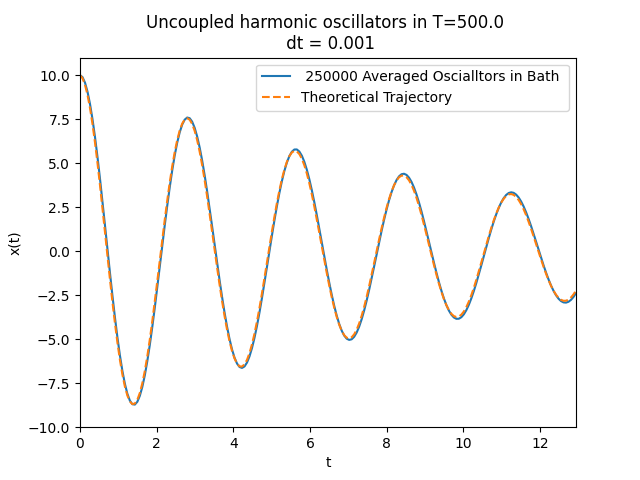
\includegraphics[width =12cm]{graphics/convharmonicmean.png}
	\end{figure}
	The mean is independent of the temperature of the bath, even though with high temperatures we would amplify the deviation from the mean, meaning the MAD and MSD which would be visible in the figure through larger deviation from the mean?
	
	We can do the same thing for the second moments of the harmonic oscillator. But since this is not absolute trivial to solve, we look at the overdamped case, which somehow(?) means that $x$ and $v$ are unambiguously linked, meaning that we can only look at $x$ since there is a unambiguous dependence of $v$ from x, leading to a equation like the first FP equation with
	\begin{equation}
		a(x,t) \overset{?}{=}	\gamma + \partial_x V(x, t)
	\end{equation}
	(No Source)
	
	For the second moment of $x$, we then get the equation
	\begin{equation}
		\partial_t \langle x^2 \rangle =	2 \frac{\gamma k_B T}{m} - 2 \frac{k}{\gamma} \langle x^2 \rangle
	\end{equation}
	(Source Aufschrieb Gernot, but unsure about coefficients)
	
	With the Solution
	\begin{equation}
		\langle x^2 \rangle (t) =	\frac{k_B T}{\gamma} \left(1 - e^{-2 \frac{k}{\eta} t}\right)
	\end{equation}
	We see that this is now dependent on the bath temperature, but it only scales the solution. Comparison with the simulation is shown in the next figure
	\begin{figure}[htp]
		\centering
		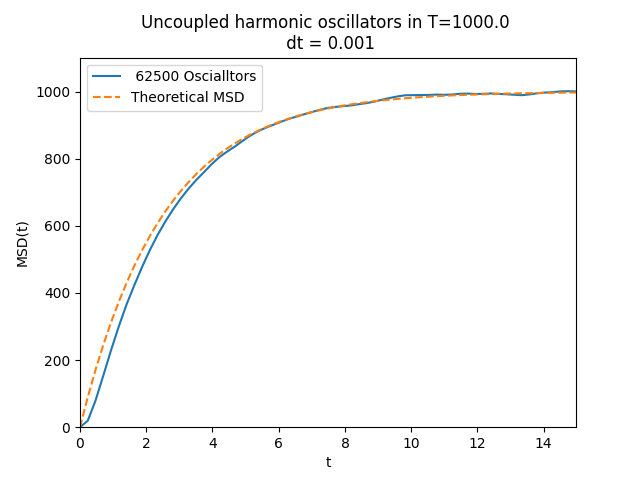
\includegraphics[width=12cm]{graphics/convharmonicmsd.png}
	\end{figure}
	The deviation for small t might be a result of the overdamped approximation.
	
	From \cite{risken1996fokker} we know the MSD for arbitrary dampening:
	\begin{align}
		\lambda_{1/2} &=	\frac{1}{2} \left(\eta \pm \sqrt{\eta^2 - 4 k}\right) \\
		\sigma_{xx}(t) &=	\frac{\eta {k_B T}}{m (\lambda_1 - \lambda_2)^2} \left[ \frac{\lambda_1 + \lambda_2}{\lambda_1 \lambda_2} + \frac{4}{\lambda_1 + \lambda_2} \left(e^{- (\lambda_1 + \lambda_2) t} - 1\right) - \frac{1}{\lambda_1} e^{-2\lambda_1 t} - \frac{1}{\lambda_2} e^{- 2 \lambda_2 t}\right]
	\end{align}
	$\sigma_{xx}$ is one diagonal entry of the $\boldsymbol{\sigma}$-matrix, which is (I think) the square root of the covariance matrix. So $=	\sqrt{\left \langle x^2\right \rangle (t)} = \sigma_{xx}(t)$ is valid.
	
	Comparing the Euler-Mayurama-Method with the BBK method we can see that the BBK method we can see that the BBK method yields much better results. While a stepsize of 0.001 is the maximum for the Euler method, a stepsize of 0.05 is still acceptable for the BBK method. Since this method does not need to generate more random numbers or evaluate the Forces more often, this translates to a huge performance boost. We also see little to no artefacts in the probability distribution for the BBK method, while we can certainly see them for the Euler method even if the stepsize is 10 times smaller.
	
	\begin{figure}[htp]
		\begin{subfigure}{0.5\textwidth}
			\centering
			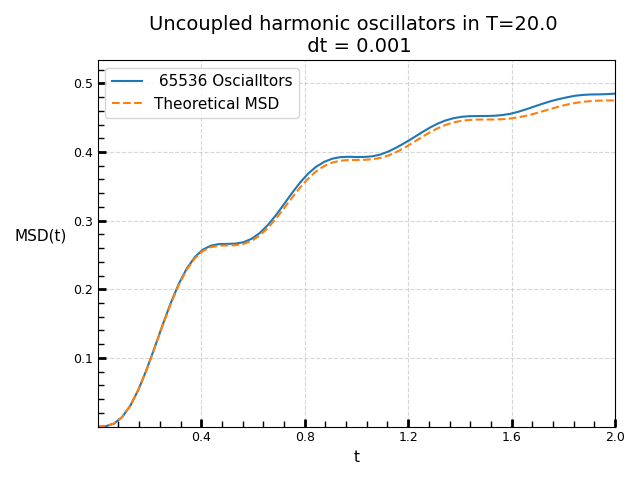
\includegraphics[width=0.8\linewidth]{graphics/MSD-Euler-0.001.png}
			\caption{Euler}
		\end{subfigure}
		\begin{subfigure}{0.5\textwidth}
			\centering
			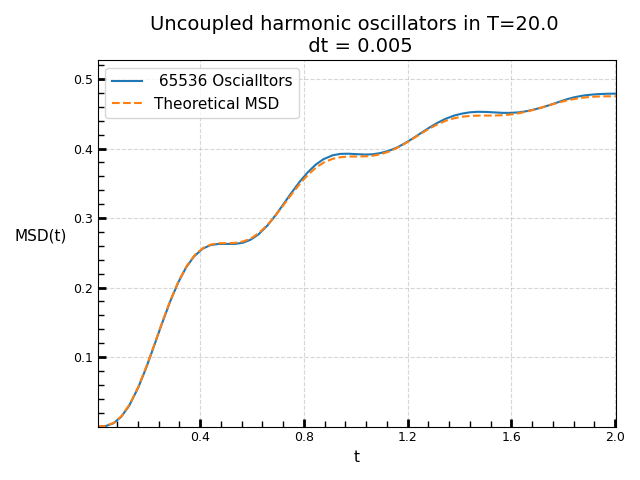
\includegraphics[width=0.8\linewidth]{graphics/MSD-BBK-0.005.png}
			\caption{BBK}
		\end{subfigure}  \\
		\begin{subfigure}{0.5\textwidth}
			\centering
			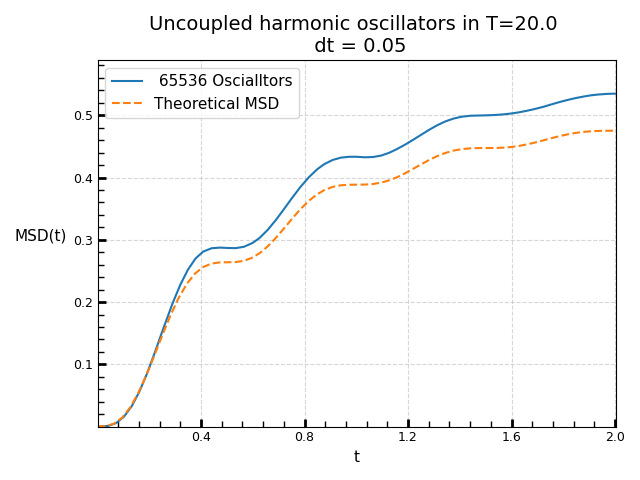
\includegraphics[width=0.8\linewidth]{graphics/MSD-Euler-0.05.png}
			\caption{Euler}
		\end{subfigure}
		\begin{subfigure}{0.5\textwidth}
			\centering
			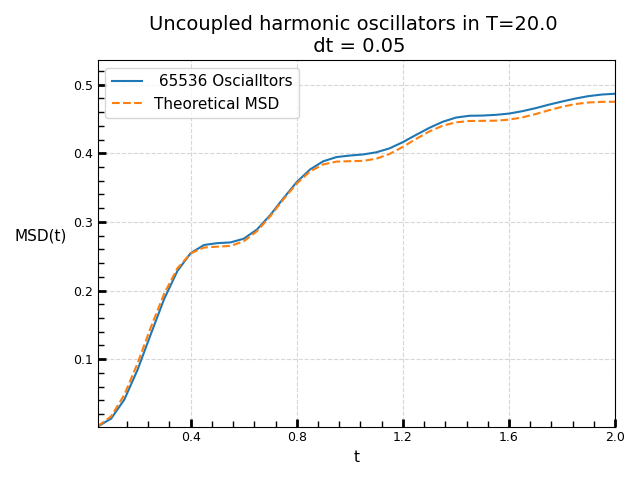
\includegraphics[width=0.8\linewidth]{graphics/MSD-BBK-0.05.png}
			\caption{BBK}
		\end{subfigure}
		\label{MSD-Comparison}
		\caption{Comparison of the calculated MSD of uncoupled harmonic oscillators for the different methods with differen Stepsizes}
	\end{figure}
	
	\begin{figure}[htp]
		\begin{subfigure}{0.5\textwidth}
			\centering
			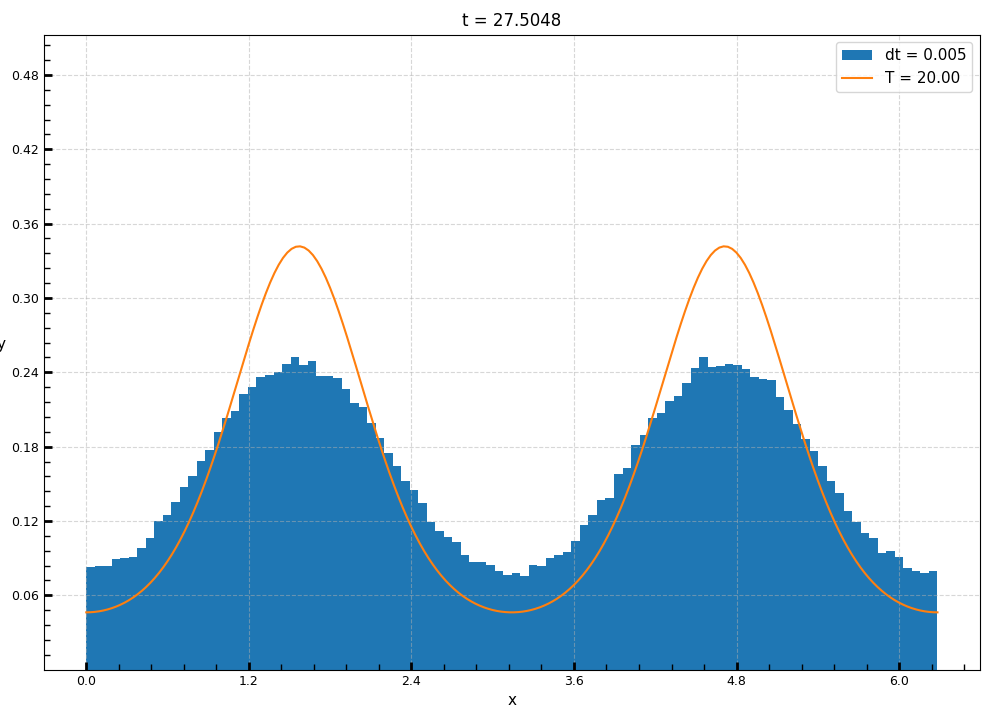
\includegraphics[width=0.8\linewidth]{graphics/Distribution-Euler-0.005.png}
			\caption{Euler}
		\end{subfigure}
		\begin{subfigure}{0.5\textwidth}
			\centering
			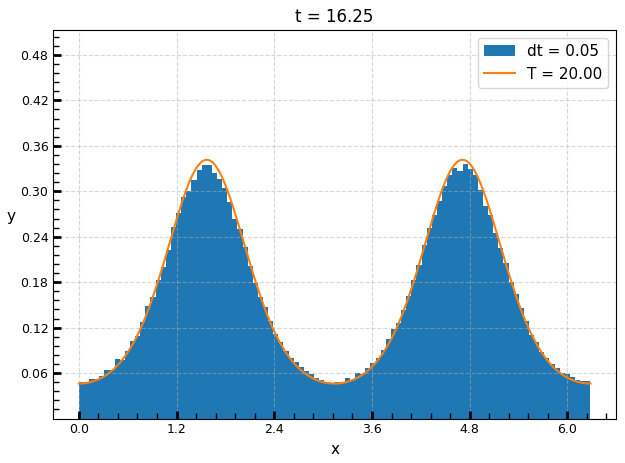
\includegraphics[width=0.8\linewidth]{graphics/Distribution-BBK-0.05.png}
			\caption{BBK}
		\end{subfigure}  \\
		\label{Dist-Comparison}
		\caption{Comparison of probability distribution of the XY model with no Interaction and a bistable cos-potential.}
	\end{figure}
	\subsection{Classical Free particles with quadratic interaction}
	In the previous section we checked for correct dynamics in a harmonic potential for uncoupled particles. Now we check for correct dynamics with free particles, but with a quadratic interaction between them.
	
	We assume the particles can move in one dimension and the interaction energy is dependent on the distance in this one dimension. The Hamiltonian of the whole system will then be
	\begin{equation}
		H(\mathbf{q}, \mathbf{p}) = \sum_i \frac{1}{2} p_i^2 + \frac{1}{2} \sum_{i, j} J (q_i - q_j)^2 + C	=	T(p_1, ..., p_N) + V(q_1, ..., q_N)
	\end{equation}
	The system is coupled to a bath and I want to calculate the partition function of this system to assess to static properties. I will have to diagonalize this hamilton to be able to evaluate the integral in the definition of the partition function. With the partition function we have access to values like the energy of the system in thermal equilibrium. The partition function for a system of N particles in one dimension is
	\begin{equation}
		Z =	\int e^{-\beta H(q, p)} d^Nq d^Np
	\end{equation}
	The integration over the impulses won't be a problem, since this is just a gaussian integral. But the integral over the interaction is another thing. The first step in diagonalizing the hamiltonian is to taylor the potential to second order around the equilibrium positions. Since
	\begin{equation}
		\frac{\partial V}{\partial q_i} = 2J \sum_j \left[(q_i - q_j) - (q_j - q_i)\right] \overset{!}{=} 0
	\end{equation}
	the system is in equilibrium for $q_i = q_j \quad \forall ~~ i, j$. I think we can w.l.o.g. set $\vec{q}^* = \vec{0}$. To make it a bit more easy for us, we only look at nearest neighbor interactions, so that we can rewrite the potential to
	\begin{equation}
		V(q_1, ..., q_N) = \sum_{i = 1}^{N} J (q_i - q_{i+1})^2
	\end{equation}
	The second order taylor expansion of a function $V: \mathbb{R}^N \rightarrow \mathbb{R}$ around the equilibrium position $\vec{q}^*$ is:
	\begin{equation}
		T_2(V(\vec{q}, \vec{q}^*)) =	\frac{1}{2} \sum_{i,j}^{N} \frac{\partial^2 V}{\partial q_i \partial q_j} (\vec{q}^*) (q_i - q_i^*) (q_j - q_j^*)
	\end{equation}
	(since we are tayloring around a minima the first order term is zero). For our potential the second derivative becomes
	\begin{equation}
		\frac{\partial^2 V}{\partial q_i \partial q_j} = V_{i, j} =	\begin{cases}
			0 \qquad  &\text{for} \quad |i - j| > 1 \\
			-2J \qquad &\text{for} \quad |i - j| = 1 \\
			4J \qquad &\text{for} \quad i = j
		\end{cases}
	\end{equation}
	As matrix form this looks like
	\begin{equation}
		U = \frac{1}{2} V_{ij} =	\begin{pmatrix}
			2J & -J & 0 &... & 0\\
			-J & 2J & -J & ... & 0 \\
			0 & -J & 2J & -J & ... \\
			... & ... & ... & ... & -J \\
			... & ... & ... & -J & 2J \\
		\end{pmatrix}
	\end{equation}
	This is the matrix that we want to diagonalize to diagonalize the hamilton. Diagonalizing means to calculate the eigenvalues and maybe the eigenvectors. The matrix $U$ luckily is a \textbf{tridiagonal toeplitz matrix}, for which the eigenvalues are known. In our case the eigenvalues become:
	\begin{equation}
		\lambda_k =	2J + 2 J \cos \left(\frac{k \pi}{N + 1}\right) \qquad \geq 0
	\end{equation}
	The eigenvectors $a_k$ to the eigenvalues are
	\begin{equation}
		(a_k)_i =	c \cdot \sin \left(\frac{k i \pi}{N + 1}\right)
	\end{equation}
	In the new coordinates $Q =	a^{-1} q$, $a$ being the matrix of the eigenvectors, the hamilton diagonalizes and we can write it as
	\begin{equation}
		H =	\frac{1}{2} \dot{Q}^T \dot{Q} + Q^T \lambda Q =	\frac{1}{2} \sum_k \dot{Q}_k^2 + \sum_k \lambda_k Q_k^2
	\end{equation}
	Now we can try to calculate the partition function. The impuls term is almost trivial:
	\begin{align}
		Z &=	\int_{-\infty}^{\infty} e^{-\beta \left(\frac{1}{2} \sum_k \dot{Q}_k^2 + \sum_k \lambda_k Q_k^2\right)} d^N\dot{Q}d^NQ = \left(\prod_k \int e^{- \frac{1}{2} \beta  \dot{Q}_k^2 } d\dot{Q}_k\right)	\left( \int e^{-\beta \left(\sum_k \lambda_k Q_k^2\right)}d^NQ\right) \\
		&= \left(\frac{2 \pi}{\beta}\right)^{N/2} 	\left( \int e^{-\beta \left(\sum_k \lambda_k Q_k^2\right)}d^NQ\right)
	\end{align}
	But with the work done diagonalizing the hamilton, the potential term can be calculated very similar:
	\begin{equation}
		Z =	\left(\frac{2 \pi}{\beta}\right)^{N/2} \left(\prod_k \int e^{- \beta \lambda_k  {Q}_k^2 } d{Q}_k\right) =		\left(\frac{2 \pi}{\beta}\right)^{N/2} \prod_k \sqrt{\frac{2 \pi }{\beta \lambda_k}} =		\left(\frac{2 \pi}{\beta}\right)^{N} \prod_k \frac{1}{\sqrt{\lambda_k}}
	\end{equation}
	With $C_N =	\prod_k \frac{1}{\sqrt{\lambda_k}}$ being a constant term depending on the system size, which should be easy to evaluate numerically. Final result:
	\begin{equation}
		Z_N =	C_N  \left(\frac{2 \pi}{\beta}\right)^{N}
	\end{equation}
	We can now calculate the mean energy via
	\begin{equation}
		\langle E_N \rangle =	- \frac{\partial \ln (Z_N)}{\partial \beta} =	- \frac{\partial}{\partial \beta} \left(\ln(C_N) + N \ln \left(\frac{2 \pi }{\beta}\right)\right) = \left( N	\frac{\beta}{2 \pi} \frac{2\pi}{\beta^2}\right) =	\frac{N}{\beta} =	N k_B T
	\end{equation}
	...Which would just be the mean energy for a system with N	particles with respectively 2 degrees of freedom?
	
	We should maybe check for other observables that depend on the coupling $J$. Since with the partition function we now now the probability distribution we can calculate arbitrary average values:
	\begin{equation}
		\langle f \rangle_N =	\int f(\vec{q}, \vec{p}) P(\vec{q}, \vec{p}) d^Nq d^Np \qquad \text{with} \qquad P_N(\vec{q}, \vec{p}) =	\frac{1}{Z_N} e^{-\beta H(\vec{q}, \vec{p})}
	\end{equation}
	Since the Hamiltonian is symmetric in $q$ and $p$, the magnetization with
	\begin{equation}
		M(\vec{q}, \vec{p}) = \frac{1}{N} \sum_i q_i
	\end{equation}
	will be zero. I	think even the MSD of the Magnetization will not depend on $J$, since the absolute position of the particles is not important for the energy. What probably should depend on $J$ would be the average distance between two spins:
	\begin{equation}
		d(\vec{q}, \vec{p}) =	\frac{1}{N} \sum_i |q_i - q_{i+ 1}|
	\end{equation}
	I could either try to evaluate the integral above numerically, or i could try to transform $Q = a^{-1} q$ again and solve it analytically.
	\subsubsection{QM particles with quadratic interaction}
	Now Hamilton Operator is
	\begin{equation}
		\hat{H}_{tot} =	\sum_{i = 1} \frac{\hat{p}_i^2}{2} + J \sum_{i = 1} (\hat{q}_i - \hat{q}_{i+1})^2
	\end{equation}
	The matrix or the eigenvalues $\lambda_k$ that diagonalize this Hamiltonian are the same as above. Meaning that we can write down the total Hamiltonian with the new coordinates
	\begin{equation}
		\hat{H}_{tot} =	\sum_{k = 1} \frac{\hat{P}_k^2}{2} + \sum_{k = 1} \hat{Q}_k \lambda_k \hat{Q}_{k} = \sum_k \hat{H}_k \qquad \text{with} \qquad \hat{H}_k =	\frac{\hat{P}_k^2}{2} + \frac{1}{2} \omega_k^2 \hat{Q}_k^2
	\end{equation}
	The transformed Hamiltonian now looks like the sum of decoupled harmonic oscillators with their own frequency $\omega_k$.
	Analogous to the quantum mechanical harmonic oscillator we can now introduce creation and destruction operators $\hat{a}^\dagger_k$ and $\hat{a}_k$ for every oscillator $k$. With those we can rewrite the Hamiltonian $\hat{H}_k$ as
	\begin{equation}
		\hat{H}_k =	\omega_k \left(\hat{a}^\dagger_k \hat{a}_k + \frac{1}{2}\right)
	\end{equation}
	The partition function for the whole system is
	\begin{equation}
		Z =	\text{Tr} \left(e^{-\beta \hat{H}_{ges}}\right)
	\end{equation}
	And it can be shown that the partition function of the whole system is just the product of the partition function of a single oscillator:
	\begin{equation}
		Z =	\prod_k Z_k \qquad \text{with} \qquad Z_k =	\text{Tr} \left(e^{-\beta \hat{H}_k}\right) =	\sum_{n_k =	0}^{\infty} \langle n_k | e^{-\beta \hat{H}_k} | n_k \rangle =	\frac{1}{e^{\frac{1}{2} \beta \omega_k} - e^{-\frac{1}{2}\beta \omega_k}}
	\end{equation}
	Now we can calculate the mean energy of the ensemble of oscillators
	\begin{equation}
		\langle E \rangle =	\text{Tr} \left(\hat{H}_{tot} \hat{\rho} \right) \qquad \text{with} \qquad \hat{\rho} = \frac{1}{Z} e^{-\beta \hat{H}_{tot}}
	\end{equation}
	Use trick with derivative:
	\begin{align}
		\langle E \rangle &=	\text{Tr} \left( \hat{H}_{tot} \frac{1}{Z} e^{-\beta \hat{H}_{tot}} \right) =	\frac{1}{Z} \text{Tr} \left( \left(-\frac{\partial}{\partial \beta}\right)e^{-\beta \hat{H}_{tot}} \right) =\frac{1}{Z}	\left(-\frac{\partial}{\partial \beta}\right) Z = - \frac{\partial \ln (Z)}{\partial \beta} \\
		&= \sum_k \frac{\partial}{\partial \beta} \ln \left(e^{\frac{1}{2} \beta \omega_k} - e^{-\frac{1}{2}\beta \omega_k}\right) =	\sum_k \frac{\omega_k}{2} \frac{e^{\beta \omega_k} + 1}{e^{\beta \omega_k} - 1}
	\end{align}
	Comparison between Classical and quantum mechanical derivation in the next figure
	\begin{figure}[htp]
		\centering
		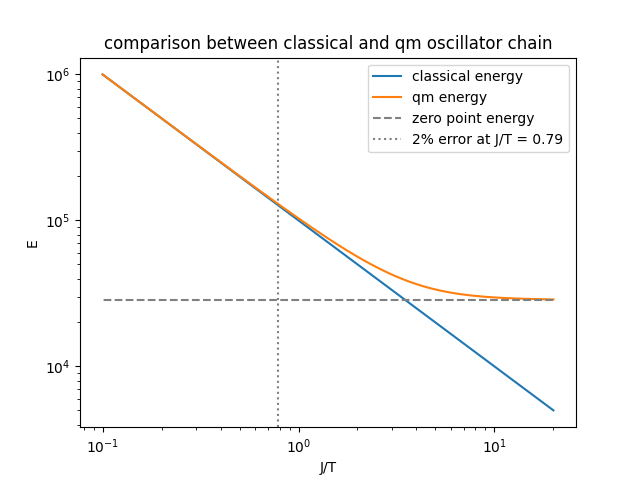
\includegraphics[width=13cm]{graphics/qmvsclassical.png}
	\end{figure}
	
	\subsection{Quenching}
	We want to do a linear Quench for starters from a defined $T_{\text{start}}$ until $T_{\text{end}}$. So we need to have an equilibrated system at $T_{\text{start}}$. We want to spend as little time as possible equilibrating, so it would surely make sense to initialize a system that already has its thermic energy. Since our system has two degrees of freedom (1 kinetic, 1 potential), the ensemble average energy will be
	\begin{equation}
		E_{\text{thermic}} =	E_{\text{pot}, \text{thermic}} + E_{\text{kin}, \text{thermic}} =	\frac{1}{2} N k_B T + \frac{1}{2} N k_B T =	N k_B T
	\end{equation}
	To initialize a system that has this energy, it is easiest to give our initial system kinetic energy that satisfies $E_{\text{kin, start}} = E_\text{thermic}$. We still want to initialize a random initial state, preferably one that is gaussian. So we can just look the mean absolute value of the impulse it we distribute it gaussian, which is the boltzmann distribution (Attention, only in 3d). The mean value of the absolute of a gaussian distributed parameter is:
	\begin{equation}
		\langle |p| \rangle =	\sqrt{\frac{2}{\pi}} \sigma
	\end{equation}
	the standard deviation of the according gaussian distribution is
	\begin{equation}
		\sigma = \sqrt{k_B T}
	\end{equation}
	We want that the starting kinetic energy satisfies:
	\begin{equation}
		E_{\text{kin, start}} =	E_{\text{thermic}} \quad \Leftrightarrow \quad \frac{1}{2} 	\langle |p| \rangle^2 = \frac{\sigma^2}{\pi}  =	k_B T_{start} \quad \Rightarrow \quad \sigma =	\sqrt{\pi k_B T}
	\end{equation}
	Meaning if we distribute our impulses with a standard deviation of $\sigma =	\sqrt{\pi k_B T}$, we should get a kinetic energy that is as large as the thermic energy.
	
	Since currently we give an amplitude to the initial state generation, it is useful to know that the gaussian distribution satisfies:
	\begin{equation}
		\alpha + \beta \mathcal{N}(\mu, \sigma^2) =	\mathcal{N}(\mu + \alpha, \beta^2	\sigma^2)
	\end{equation}
	Which means $\sigma$ will just be the amplitude of our initialization $p_0 = \sigma$
	
	\section{Analysis}
	\subsection{static critical exponents}
	An important classification of our system would be to calculate the critical exponents. One of the most vital critical exponents for us would be $\nu$, since it shows how the correlation length scales with the (reduced) temperature:
	\begin{equation}
		\xi =	\frac{\xi_0}{\varepsilon^\nu}
	\end{equation}
	This static scaling is valid for systems in equilibrium. We could find out $\nu$ numerically by simulating systems at constant temperature, let them equilibrate and then calculating the correlation length. In principle, it should not matter with what initial state we begin the equilibration, so we might have 3 possibilities:
	\begin{itemize}
		\item high energy initial state with $E_{System} \gg E_{thermal}$
		\item thermal state with $E_{System} \approx E_{thermal}$
		\item low energy state with $E_{System} \ll E_{thermal}$ or $E_{System} =0$
	\end{itemize}
	For temperatures significantly above the critical temperature, it should not matter which initial state we choose, but for Systems below the critical temperature at least the low energy state will probably not be practical since the system won't have the energy to surpass the potential barrier and therefore will take a really long time to equilibrate.
	
	The computational difficulty is that the equilibration will take a really long time around the phase transition, as it is described by the critical slowdown, and the correlation length exceeds the system size, which makes the computation really expensive.
	
	We should probably try to start from above $T_c$ and increase our system size as we approach the critical temperature.
	
	Using the finite size methods described in the last part of the section \hyperref[withoutsecRG]{Renormalization Group methods}, we try to extract the static critical exponent of our system.
	
	\begin{figure}[ht]
		\begin{subfigure}{0.5\textwidth}
			\centering
			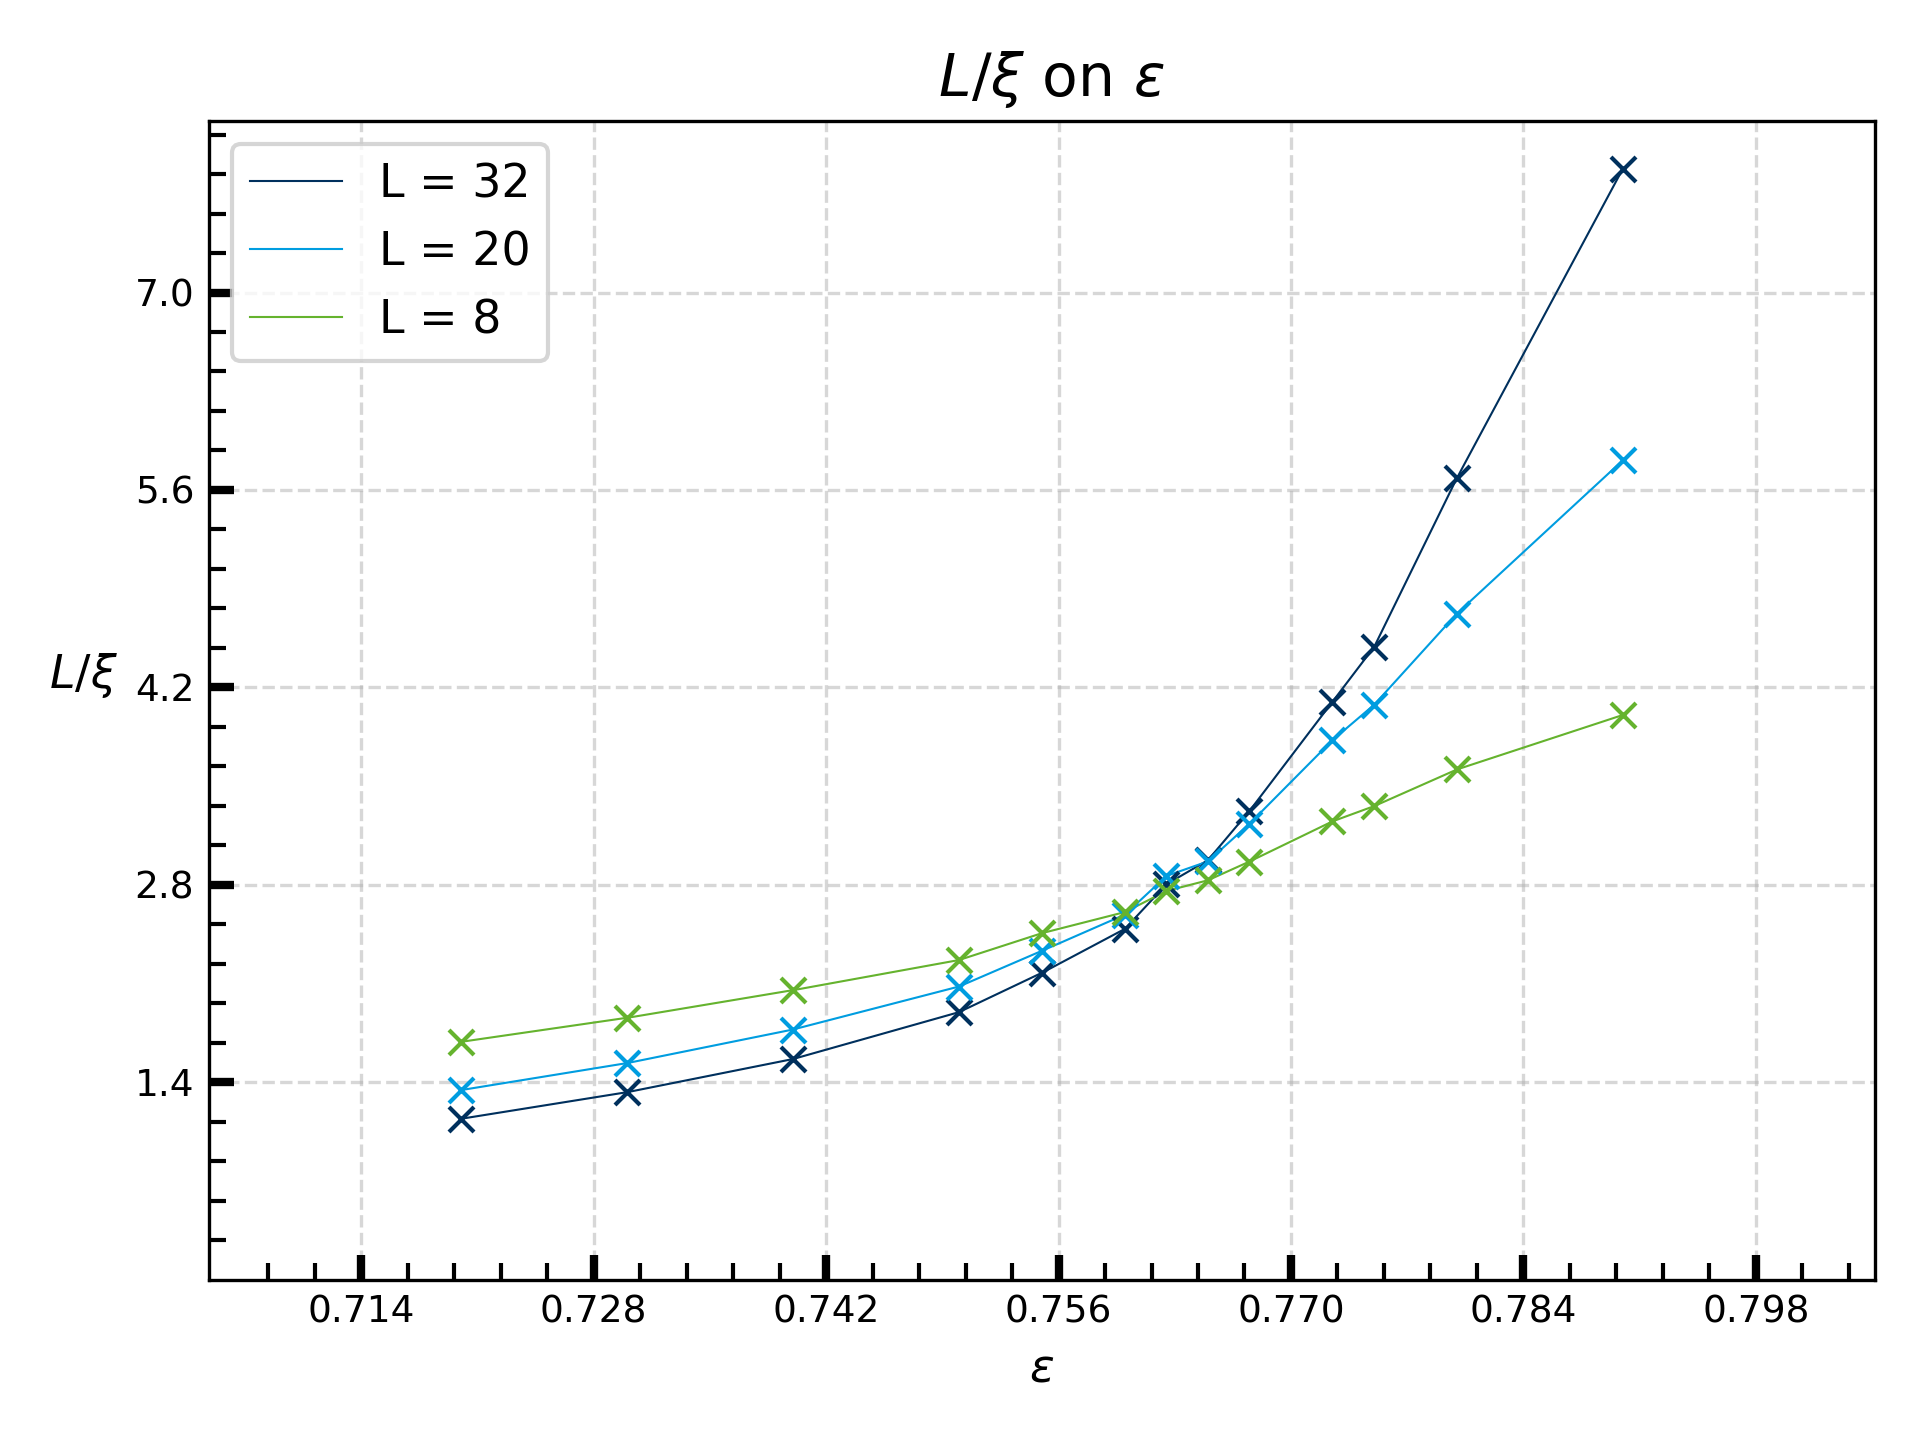
\includegraphics[width=0.8\linewidth]{graphics/L_xi.png}
			\caption{$\frac{L}{\xi}$ on reduced temperature for different system sizes}
		\end{subfigure}
		\begin{subfigure}{0.5\textwidth}
			\centering
			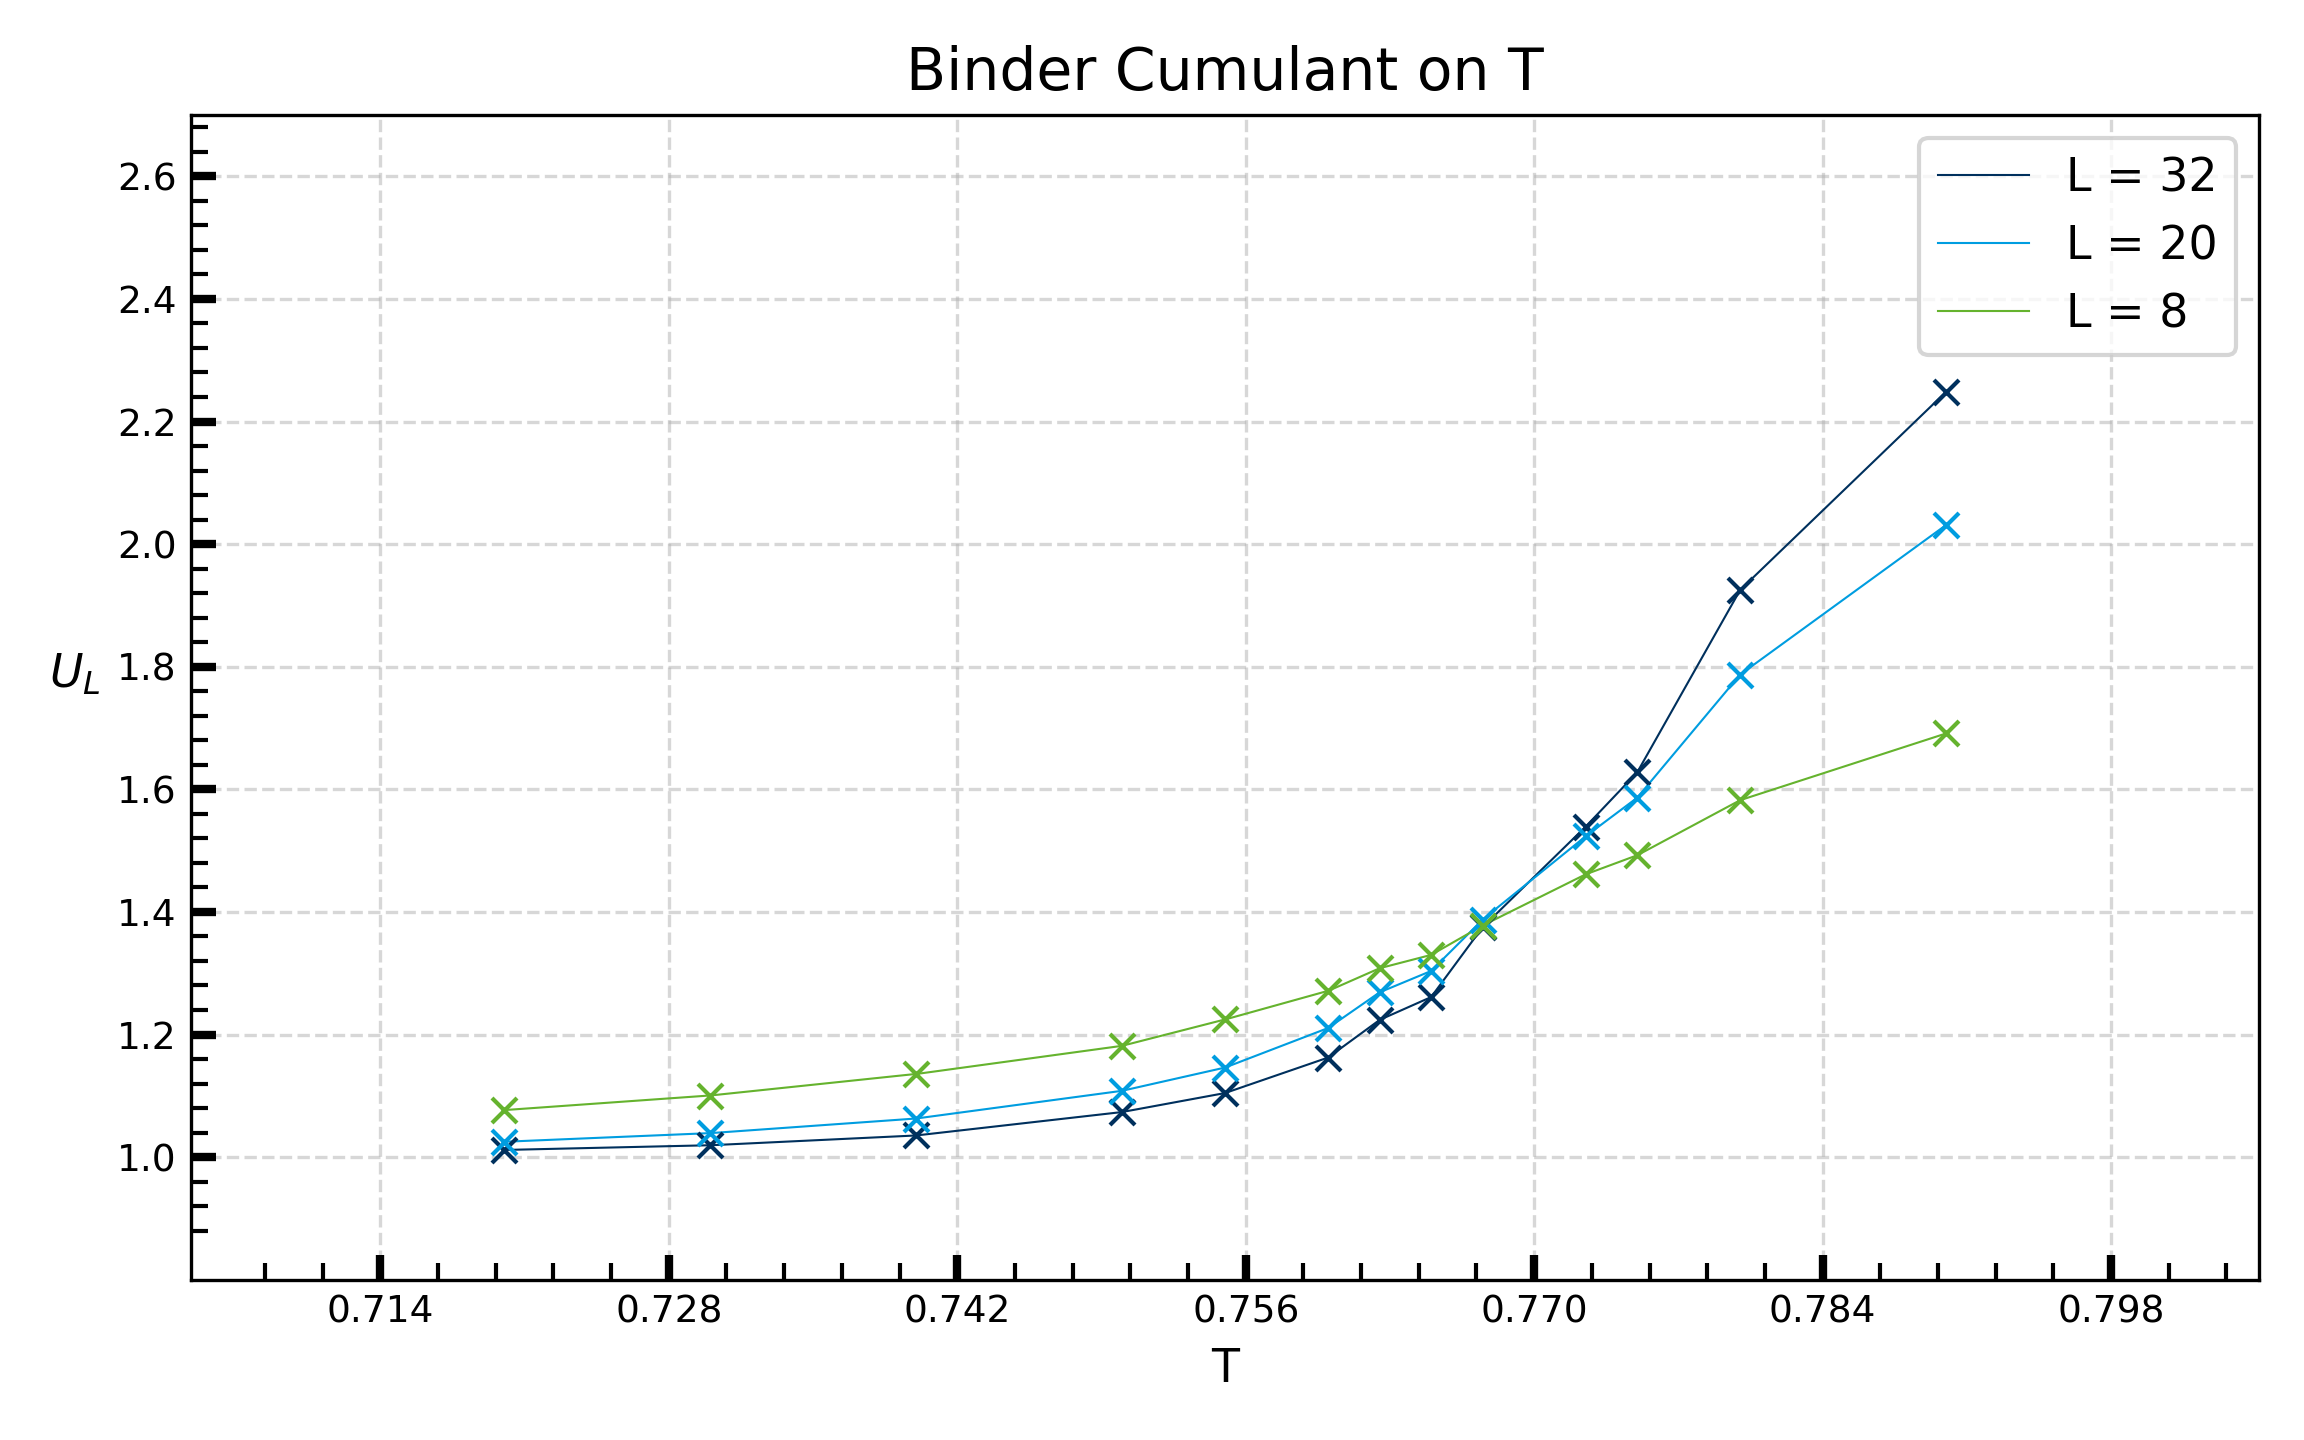
\includegraphics[width=0.8\linewidth]{graphics/cum2.png}
			\caption{$\frac{L}{\xi}$ on reduced temperature for different system sizes}
		\end{subfigure} \\
		\begin{subfigure}{0.5\textwidth}
			\centering
			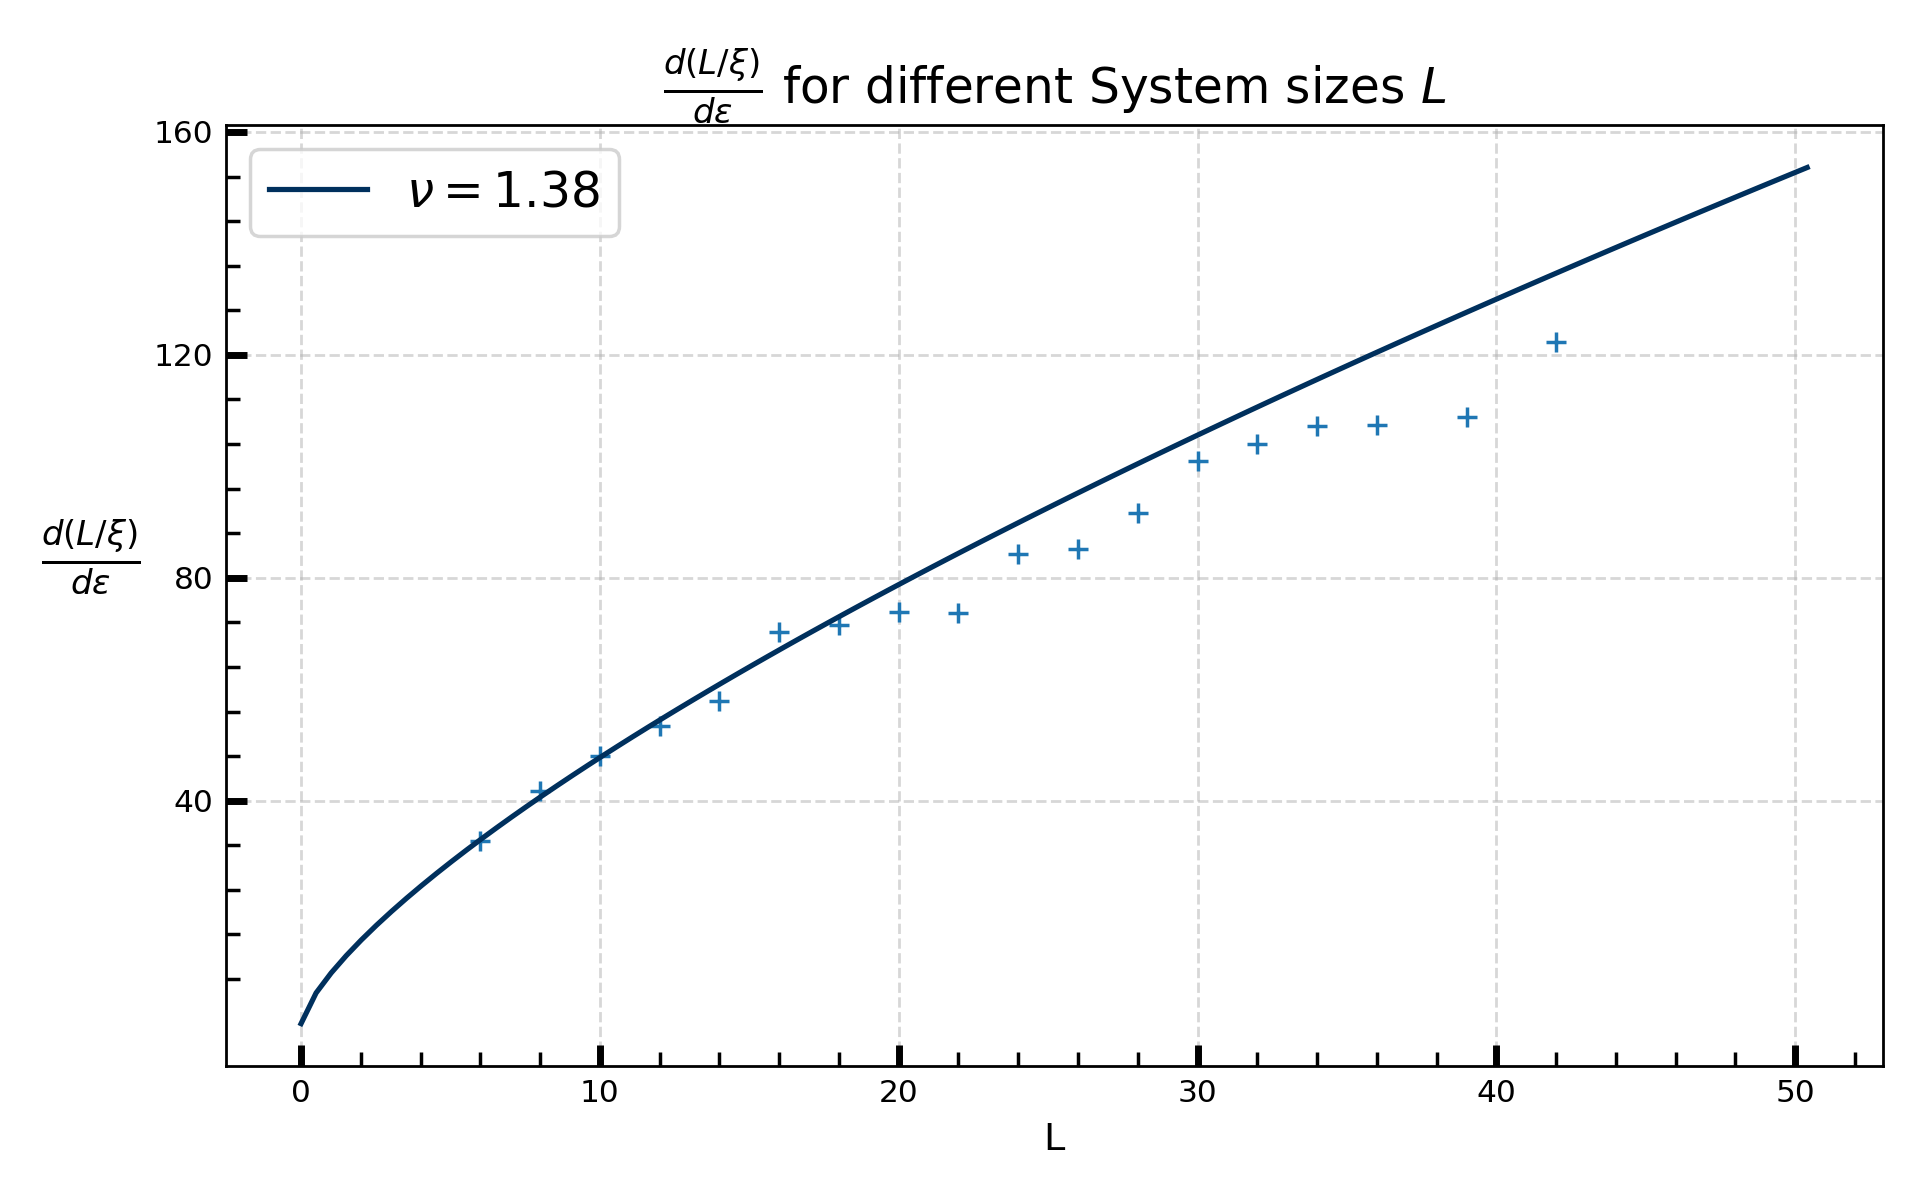
\includegraphics[width=0.8\linewidth]{graphics/critical exponent L_xi.png}
			\caption{$\frac{L}{\xi}$ on reduced temperature for different system sizes}
		\end{subfigure}
		\begin{subfigure}{0.5\textwidth}
			\centering
			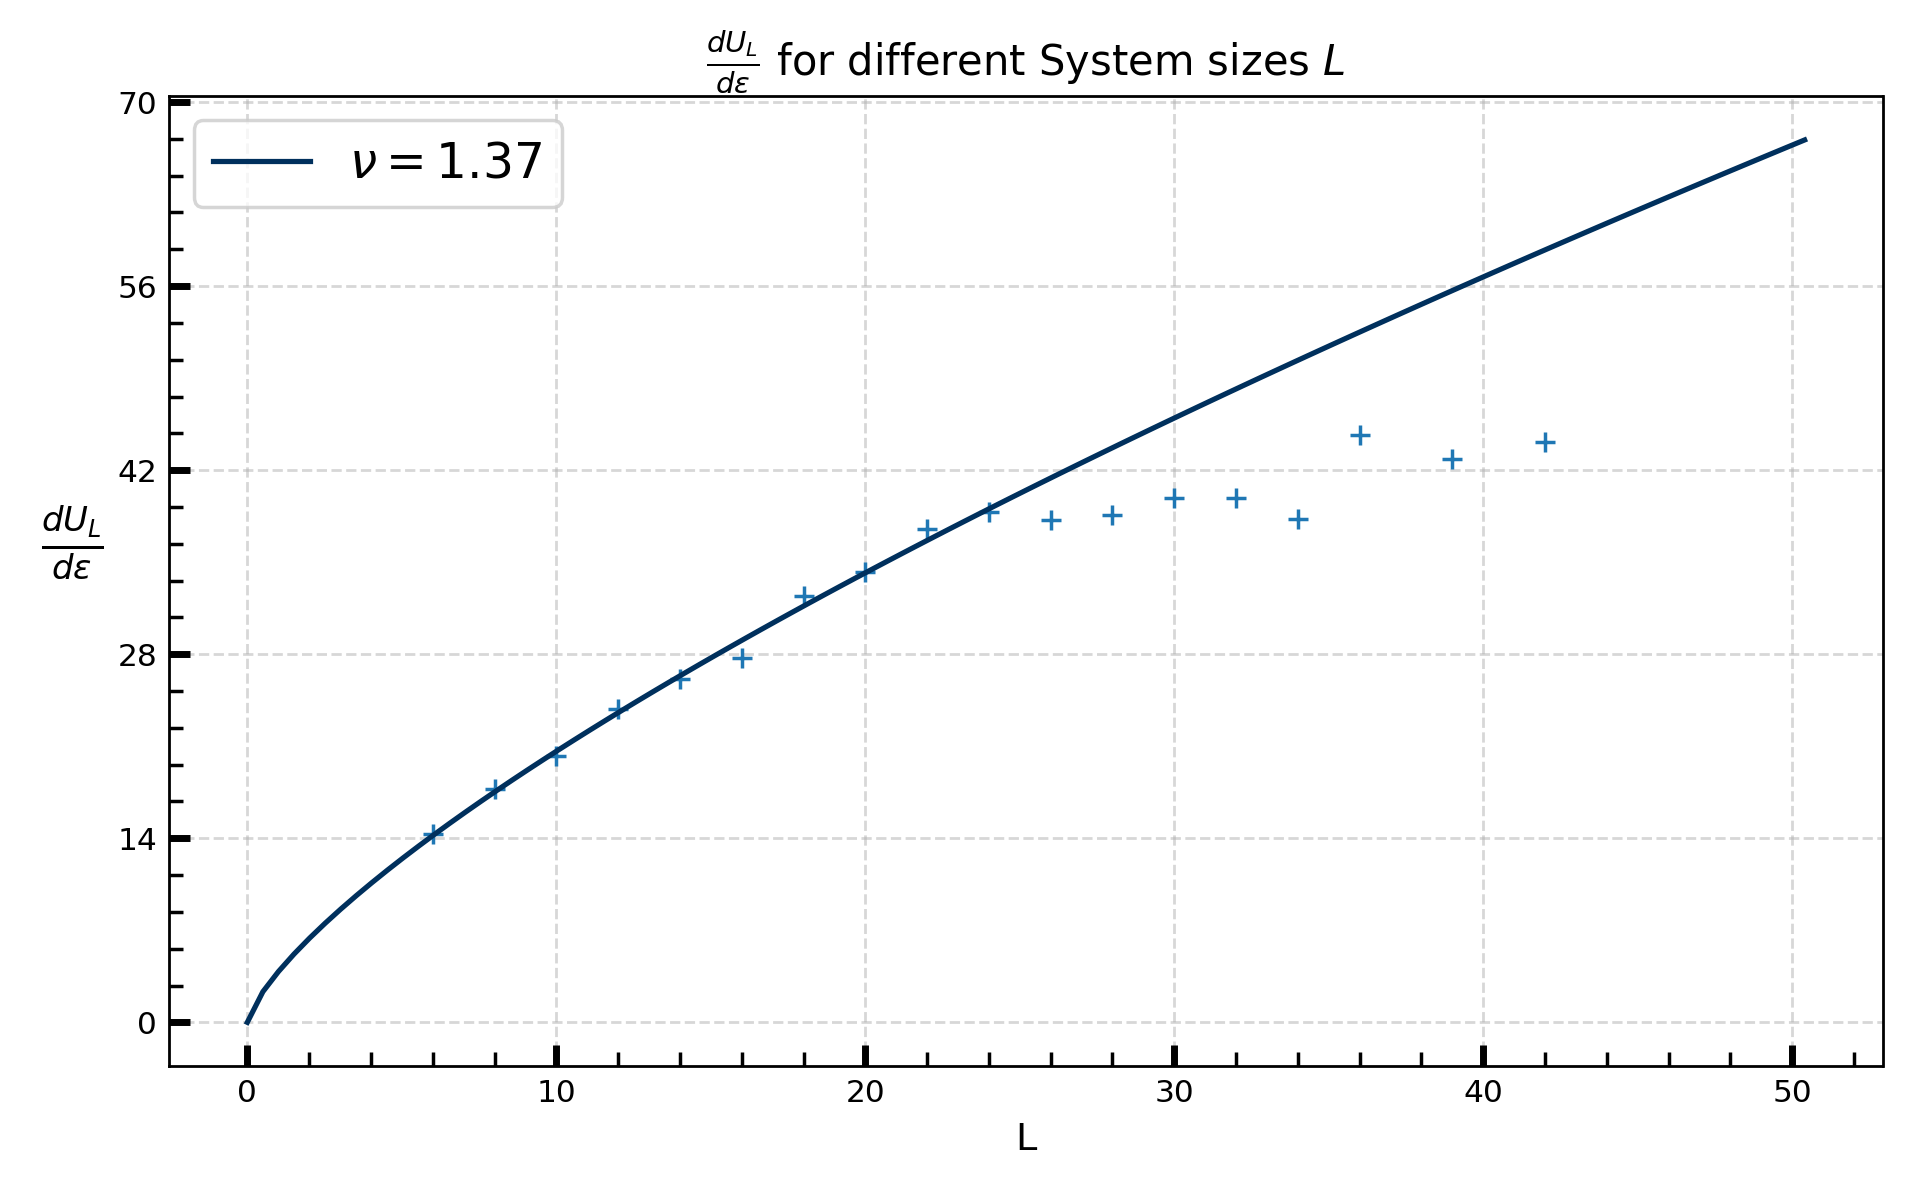
\includegraphics[width=0.8\linewidth]{graphics/critical exponent U_L.png}
			\caption{$\frac{L}{\xi}$ on reduced temperature for different system sizes}
		\end{subfigure}
		\caption{Finite size methods for the phenomenological couplings $\frac{L}{\xi}$ and $U_L$}
	\end{figure}
	Considering only small system sizes where we can be sure that our system equilibrated during our time of simulation, we obtain a critical exponent of $\nu = 1.38$, which is significantly higher than the expected one for the Ising-model, which would be $\nu  = 1$.
	
	\begin{table}
		\begin{center}
			\begin{tabular}{ccc}
				\centering
				& Our Model & 2D Ising \\  [0.5ex]
				\hline
				$\nu$ & 1.37 & 1 \\
				$z$ & 1.90 & 2.15 \\
				$\frac{\nu}{1 + \nu z}$ & 0.38 & 0.32
			\end{tabular}
			\caption{Comparison between the expected 2D Ising critical exponents and the extracted critical exponents of our model}
		\end{center}
	\end{table}
	
	\subsection{dynamic critical exponent}
	Using the relations between the correlation length and the quench timescale of section \hyperref[KZM]{Kibble-Zurek Mechanism}, we can extract the correlation length and perform a linear fit to extract $\frac{\nu}{1 + \nu z}$. Seen in \autoref{Fig:z-Extraction}.
	
	\begin{figure}[ht]
		\begin{subfigure}{0.5\textwidth}
			\centering
			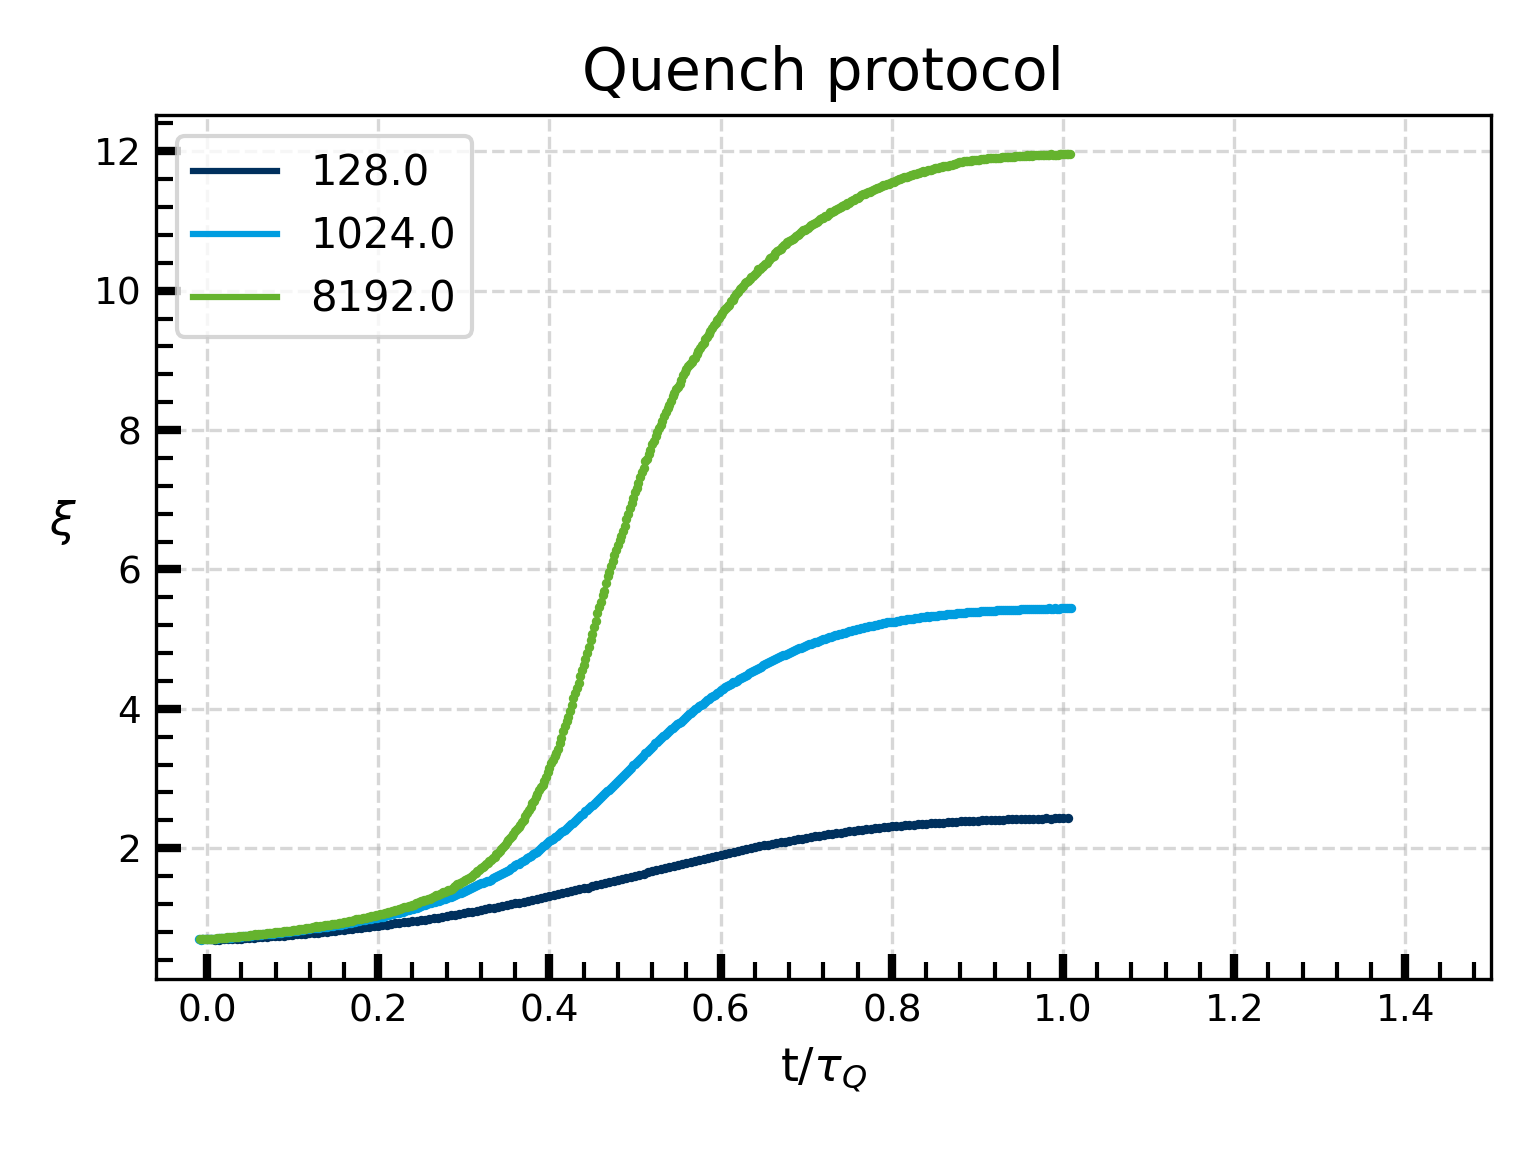
\includegraphics[width=0.8\linewidth]{graphics/quench process.png}
			\caption{averaged ${\xi}$ on time for different quench timescales}
		\end{subfigure}
		\begin{subfigure}{0.5\textwidth}
			\centering
			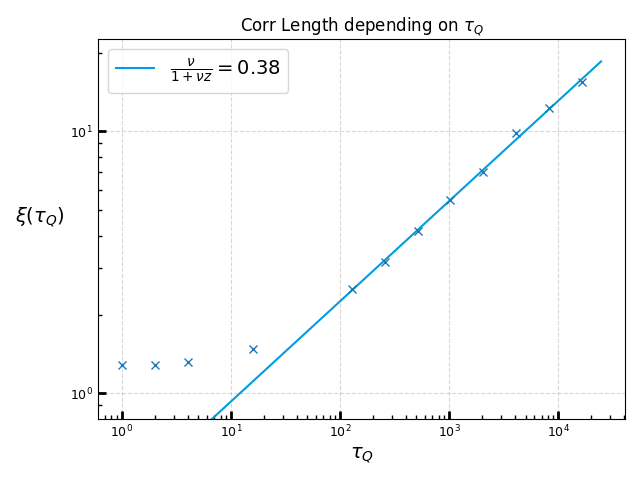
\includegraphics[width=0.8\linewidth]{graphics/critical exponent z.png}
			\caption{final correlation length ${\xi}$ on the quench timescale}
		\end{subfigure}
		\caption{\label{Fig:z-Extraction}Our system is linearly quenched and its correlation length is extracted for multiple times and quench timescales}
	\end{figure}
	We can see that for very small timescales the $\xi$-scaling predicted by the Kibble-Zurek mechanism is not valid and the quench is so fast that the system is no able to adapt at all. This is probably because the quench timescale is small compared to the equilibration time even far away from the phase transition so that the system freezes instantly and we do not see any change in the correlation length at all.
	Summary of the most important points and what I am doing. For more detailed Information you can look into the sections.
	
	We look at a 2D isotropic lattice, denoting each site with its row and column number $(i,j)$. Every lattice site inhibits a dimer, which can be inclined and has an inclination angle $\vartheta_{i, j}$. The inclination angle is confined ($\vartheta \in \left[-\frac{\pi}{2}, ~\frac{\pi}{2}\right)$), and since we want to simulate the dynamics of the system with SDEs, we either need to project the inclination angle on the said interval every step, or we work with a transformed coordinate $\vartheta_{i, j} \rightarrow q_{i, j}$ (More about this transformation in Section Model, System).
	
	The inclination angle has in the ordered phase two minima /	equilibrium positions, so we want to model $\vartheta_{i, j}$ to live in a double well potential, which is equivalent to $q_{i, j}$ living in a double well potential. The double well potential is of the form
	\begin{equation}
		V_{DW}(q) = \frac{1}{2}	\alpha \left(q^4 - \beta q^2 \right) \qquad \Rightarrow \qquad 	F_{DW}(q) =	\frac{\partial V}{\partial q} =	\alpha \left(2q^3 - \beta q \right)
	\end{equation}
	More about the potential in section Model, Potential.
	
	The Dimers interact, which leads to the proposal of an interaction potential. We for now assume that only nearest neighbors (NN)  interact. The angle-nature of the system and parallels to the XY-Model lead me to the proposal of a cosine interaction:
	\begin{align}
		V_I(\lbrace q_{i, j}\rbrace_{NN}) =	~~&J_{\parallel} \left(\cos\left( q_{i, j} - q_{i, j-1}   \right) + \cos\left(    q_{i, j} - q_{i, j+1}\right) \right) \\
		+ &J_{\perp} \left(\cos\left( q_{i, j} - q_{i-1, j}   \right) + \cos\left(    q_{i, j} - q_{i+1, j}\right) \right)
	\end{align}
	\textbf{Important:} I earlier realized that this is horribly wrong when using the transformed coordinate instead of the angle. The difference of the transformed coordinates can exceed the period.
	
	This leads to the total potential
	\begin{equation}
		V(\lbrace q_{i, j}\rbrace_{NN}) =	V_{DW}(q_{i, j}) + V_I(\lbrace q_{i, j}\rbrace_{NN})
	\end{equation}
	
	We want to simulate the system using stochastic differential equations, or more precisely, Langevin-equations (More on that in the Section ''Langevin Equations''). They are of the form
	\begin{equation}
		X(t + dt) =	X(t) + A(X(t), t))dt + D^{1/2}(X(t), t) N(t) (dt)^{1/2}
	\end{equation}
	In our case, $X(t)$ represents the derivative of the transformed inclination angle, the transformed angle velocity so to say, called $p_{i, j}$ from now on. The Drift Function for us consists of the dampening part and the part resulting out of the above described potential. The Diffusion part results out of a thermic coupling of the dimers on the surface to the bulk of the silicon probe. They have the form:
	\begin{equation}
		A(q_{i, j}, p_{i, j}, t) = - \eta p_{i, j} - \frac{\partial V(\lbrace q_{i, j}\rbrace_{NN})}{\partial q_{i, j}} \qquad \text{and} \qquad D^{1/2}(t) =	\sqrt{2\eta T(t)}
	\end{equation}
	Plugging this into the Langevin-equation yields a first order system for our transformed coordinate and impuls:
	\begin{align}
		&(I)  ~~~&&q_{i, j}(t + dt) = q_{i, j}(t) +	p_{i, j}(t) dt  \\
		&(II) &&p_{i, j}(t + dt) = p_{i, j}(t)- \left(\eta p_{i, j}(t) + \frac{\partial V(\lbrace q_{i, j}\rbrace_{NN}(t))}{\partial q_{i, j}}  \right) dt		+ \sqrt{2 \eta T(t)} n \sqrt{dt}
	\end{align}
	with n being a sample value of $\mathcal{N}(0, 1)$.
	
	$T(t)$ is the bath temperature and therefore an important parameter for the phase transition. For high $T > T_c$, the influence of the dissipation term is so large, that the double well character of the potential is not important and the dimers behave as if they lived in a parabolic potential. For very small temperatures $T < T_c$, the kicks that the system gets from the bath won't be large enough to escape one of the minimums (at least not for long times) and so the dimer has to settle into one of the two. Which one is now determined by the Interaction during the cooling of the bath. At $T =	T_c$, the kicks are still strong enough so that ''the dimers can draw one another into the same minimum'' and therefore induce some ordering in form of patches of same or antiparallel orientation. The timescale on which we pass the critical temperature now determines how large those patches are, which is exactly the Kibble-Zurek-mechanism. The cooling atm is linear:
	\begin{equation}
		T(t) =	\max\left(T_{start} - \frac{t}{\tau}, T_{end}\right)
	\end{equation}
	A typical Quench with initial conditions $q_{i,j} =	0, p_{i, j} =0$ then looks like in the upcoming figure.
	
	\begin{figure}[t]
		\centering
		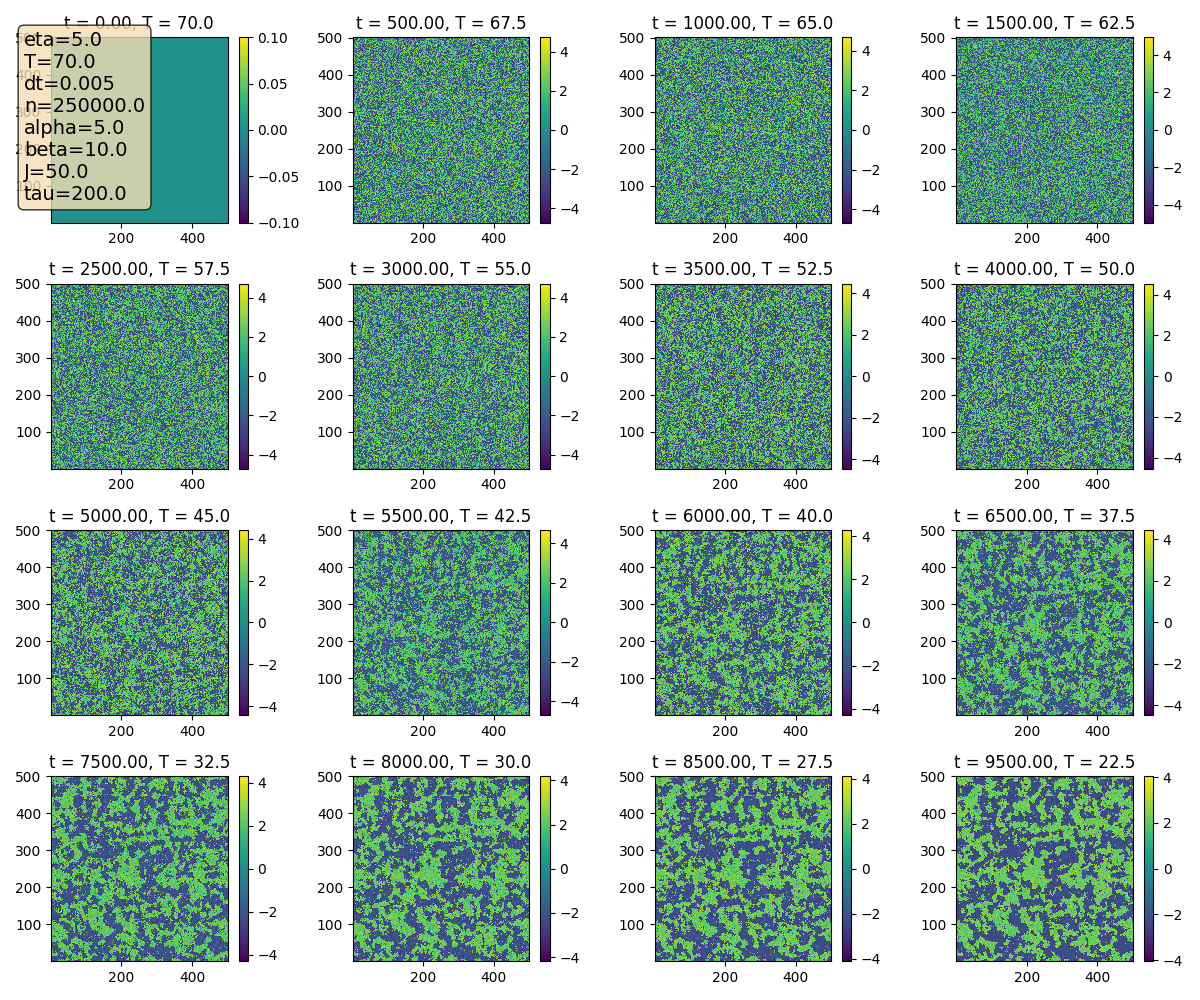
\includegraphics[width=13cm]{graphics/500x500.png}
	\end{figure}
	In this figure, it looks like the phase transition occurs somewhere around $T_c =	50 - 40$, which is not in accordance with the estimation in System, potential section.
	
	After doing the simulation, we need to extract the correlation length to find out how the the defect density is scaling. The way I do this at the moment is the following:
	The correlation function is defined as:
	\begin{equation}
		C(q,s) =	\langle \sigma_{i,j} \sigma_{i +q ,j +s} \rangle = 	\frac{1}{m \cdot n} \sum_{i, j} \sigma_{i,j} \sigma_{i +q ,j +s}
	\end{equation}
	We know that the two-point-correlation function exponentially decays with the distance between the two sites:
	\begin{align}
		&C(q, 0) =	C_x(q) = \langle \sigma_{i,j} \sigma_{i +q ,j} \rangle \sim \frac{f_x}{q^{\vartheta_\gtrless}} 	e^{-q /	\xi_x} \qquad \\
		&C(0, s) =	C_y(s) =	\langle \sigma_{i,j} \sigma_{i ,j + s} \rangle \sim \frac{f_y}{s^{\vartheta_\gtrless}} 	e^{-s /	\xi_y} \qquad
	\end{align}
	The Fourier Transform of the Correlation function is called the structure factor, and for exponential decay the fourier transform is a lorentzian peak, or more accurately for the Correlation function in x direction:
	\begin{equation}
		C_x(q) \sim e^{-q /	\xi_x} \qquad \Rightarrow \qquad \Re\left(\tilde{C}_x(k)\right) = \Re \left(S_x(k) \right) \sim \frac{2 \xi_x}{1 + 4 \pi^2 k^2 \xi_x^2}
	\end{equation}
	If we can calculate the Structure factor, we can extract the width of its peak and therefore calculate the correlation length.
	We can also show, that the Structure factor is proportional to the averaged/summed absolute squared value of the fourier transform of the lattice:
	\begin{align}
		\langle |\tilde{\sigma}_{k, l}|^2 \rangle_x &=	\frac{1}{N_x} \sum_k  |\tilde{\sigma}_{k, l}|^2 \overset{?}{=} \sum_{i, j} \sum_q \sigma_{i, j}\sigma_{i, j+s} e^{2\pi \mathrm{i} \frac{sl}{N_y}} \overset{(0.63)}{=} N_x N_y \sum_q C(0, s) e^{2\pi \mathrm{i} \frac{sl}{N_y}}	\\
		&= N_x N_y \tilde{C}_x^*(l) =	N_x N_y S_x^*(l)
	\end{align}
	$\langle ~ \cdot~ \rangle_x$ denotes averaging over the x direction. In my implementation, the average is directly proportional to the structure factor and not to the complex conjugate. In 0.66 it looks like I should only look at the real part of the structure factor? But in 0.67 we can see that the structure factor should be real anyway? Fourier transforming an exponential decay actually yields an imaginary part in addition to the lorentzian peak.
	
	$\tilde{\sigma}_{k, l}$ is the 2D fourier transform of the lattice, defined by
	\begin{equation}
		\tilde{\sigma}_{k, l} =	\sum_{i = 0}^{n-1} \sum_{j =	0}^{m - 1} \sigma_{i,j}  e^{-2\pi \mathrm{i} \left(\frac{ik}{n} + \frac{jl}{m}\right)}
	\end{equation}
	
	If i calculate $S_x(l)$ and $S_y(k)$ through transformation of the lattice, for a single trajectory/lattice I get something like in the next figure.
	\begin{figure}
		\centering
		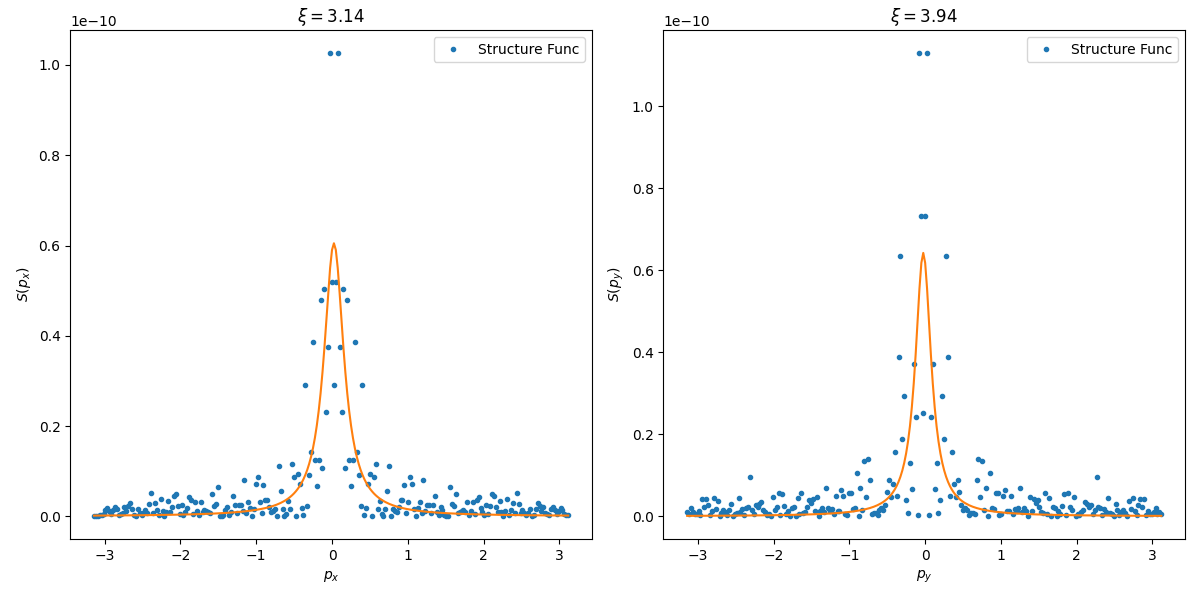
\includegraphics[width=13.5cm]{graphics/structfunc.png}
	\end{figure}
	We can see that the Structure factor is oscillating pretty heavily. My next step will be to average over multiple lattices.
	
	More detailed info on the correlation length can be found in the ''Correlation Function and Correlation Length'' section.
	
	\mainmatter
	\renewcommand{\chapterautorefname}{Chapter}
	\renewcommand{\sectionautorefname}{Section}
	\chapter{Introduction}
	\section{Motivation}
	In the area of semiconductor technology, silicon has become the cornerstone material driving the innovations that power our modern world. Its versatility, reliability, and abundance have solidified its position as the basic building block of the semiconductor industry, making silicon responsible for large parts of the recent human revolution. Its semiconducting properties facilitate the creation of wafers and integrated circuits, which are the centerpieces of computers, smartphones, and virtually any recent electronic device. \\
	
	The most important part of integrated circuits are transistors. They function as switches which make up binary numbers and logic gates that every processor uses to do math. The speed at which processors perform calculations is majorly influenced by the number of transistors available. Therefore the pursuit of further miniaturization is crucial for performance enhancement. Up-to-date transistors approach wire diameters of about $5\text{ nm}$. (reference?) This is close to atomic scales as the diameter of a silicon atom and the lattice constant are around $0.2\text{ nm}$ or $0.55 \text{ nm}$ respectively. At these scales surface effects play an ever-increasing role in influencing the behavior and conductivity of the wires. Indeed manufacturers have difficulties controlling the current flow through the channels of the transistors. Hence a better understanding of the behavior of the surface is critical to ensure progress in classical computing. \\
	
	Specifialy the Si(001) surface of monocrystalline silicon is important because it forms an interface with the oxide layer in transistors, that isolates silicon wires from their environment. Also wafers are cut along the Si(001) surface. The orientation of the cut is important since many of a crystal's structural and electronic properties are highly anisotropic. \\
	
	The Si(001) surface undergoes an order-disorder phase transition between two surface reconstructions. While static properties like possible reconstructions, their energies and electronic structures are thoroughly investigated, the dynamic properties are not yet well understood. A rich dynamic phenomenon to consider is the Kibble-Zurek mechanism which describes the unavoidable non-adiabatic evolution of systems as they cross phase boundaries. The quench time is directly related to the number of domains of different order which in turn influence the electronic properties of the surface. \\
	
	\section{Thesis Structure}
	This thesis aims to contribute to the understanding of the dynamic behavior of Si(001) during a quench. The already existing discrete Ising-like description of the surface is extended to a continuous XY-like model and adapted to the silicon surface. Well established molecular dynamics methods are used in combination with state-of-the-art parallel programming and GPU acceleration techniques to overcome the numerous numerical obstacles that are inherent to the nature of phase transitions. The used Langevin-type stochastic differential equations are motivated from a quantum mechanics point of view. Renormalization group techniques are employed to set a theoretical baseline for the investigation of the phase transition. \\
	
	\autoref{Section::Silicon} firmly concludes the current viewpoint on and knowledge of the Si(001) surface and its order-disorder phase transition. \autoref{Chapter::Phase-Transitions} explores the renormalization group description of phase transitions to create a theoretical understanding for what follows. It introduces the concept of universality and the methods of finite size scaling which are used to investigate and interpret the simulation results.  \autoref{Chapter::Simulating-Dynamics} explains the used numerics and motivates our description from a quantum point of view. Moreover, the XY model used to describe the Si(001) surface is introduced and investigated. The results of various investigations like dynamic quenches, but also static measurements are written in \autoref{Chapter::Implementation-Results}. In \autoref{Chapter::Summary-Lookout} the main points of the thesis are summarized and an outlook for possible further research is given. The appendix contains calculations to various parts of the work as well as benchmarks for the simulation. \\
	
	The simulation is written in \texttt{C++} using \texttt{CUDA} \cite{cuda} and \texttt{Thrust} \cite{thrust}. The evaluation and plotting is done in \texttt{python}. The whole source code can be obtained at \texttt{github.com}.
	
	The surface is semiconducting \cite{himpsel1979photoemission, uhrberg1981experimental, handa1989plasma} \\
	
	
	\chapter{The Si(001) Surface} \label{Section::Silicon}
	\section{Surface Reconstruction}
	Below a temperature of $T =	1687~\text{K}$ silicon crystallizes in a diamond cubic crystal structure as shown in \autoref{Fig::SiliconDiamond} with a lattice constant of $a =	5.431~\text{\AA} $ \cite{tiesinga2021codata}. When cutting this crystal structure along the crystallographic (001) plane, the resulting system exhibits a surface reconstruction. Surface atoms are left in a high-energy state with two dangling bonds. One of those bonds can be invested into forming a dimer with the neighboring Si atom in (110) direction \cite{chadi1979atomic}, which, as shown by theoretical calculations \cite{ramstad1995theoretical, batra1990atomic, dabrowski1992self}, leads to a large reduction of surface energy of roughly $1.8~\text{eV}$ per dimer.
	\begin{figure}[htp]
		\centering
		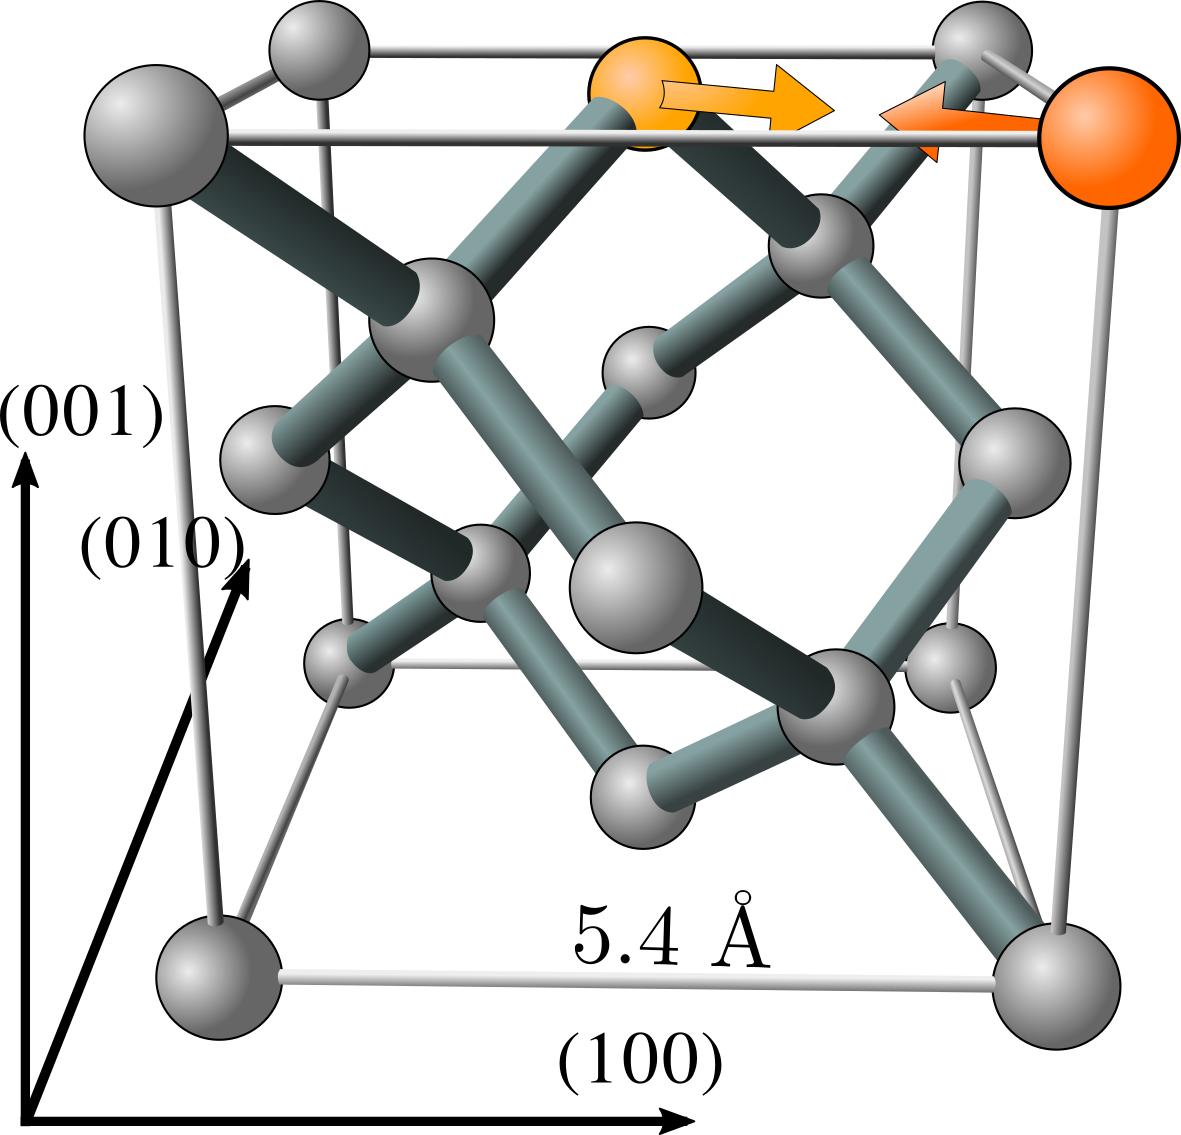
\includegraphics[width=0.5\linewidth]{graphics/Sili.png}
		\caption{The crystalline structure of Si in its solid state is shown \cite{sistrucure}. The orange colored atoms form a dimer when cutting the diamond structure along the (001) plane. The coordinate system axis are denoted by their Miller indices and normal to their corresponding crystallographic planes. The orange silicon atoms dimerize during reconstruction of the (001) surface.}
		\label{Fig::SiliconDiamond}
	\end{figure}
	
	The resulting dimers can further reduce their energy by vertical buckling. The dimers tilt to an angle of about $18^\circ$ \cite{ramstad1995theoretical, pillay2004revisit}, which lowers the surface energy by another $0.15~\text{eV}$ \cite{inoue1994order} per dimer. A charge transfer of approximately $0.1 e$  \cite{brand2023critical, landemark1992core} is induced by the buckling. The electrostatic interaction of the dimers is characterized by a coupling strength $J$. The surface reconstruction with the lowest energy was through theoretical \cite{ramstad1995theoretical, pillay2004revisit, inoue1994order, brand2023critical} and experimental (low energy electron diffraction \cite{matsumoto2003low, kubota1994streak, brand2023critical} and scanning tunnel microscope \cite{wolkow1992direct, tochihara1994low})  methods found to be the $c(4\times 2)$ reconstruction, shown in \autoref{Fig::dimer-configs} (b). It minimizes the interaction energy as well as the surface stress. The alternative buckling in both directions suggests an antiferromagnetic interaction along $(110)$, $J_\parallel$, and across $(1\overline{1}0)$, $J_\perp$, the dimer rows, but the interaction across the row is actually ferromagnetic. However, the dimer interactions are strongly anisotropic with $J_\parallel$ being much larger than $J_\perp$ which causes a guaranteed alternating buckling in $(110)$ direction. The ferromagnetic diagonal interactions $J_\times$ overpower $J_\perp$ so diagonal alignment is preferred, which in turn implies anti-alignment in $(1\overline{1}0)$ direction. It has been suggested that the interaction is of dipole kind \cite{pillay2004revisit}.
	\begin{figure}[htb]
		\begin{subfigure}{0.5\textwidth}
			\centering
			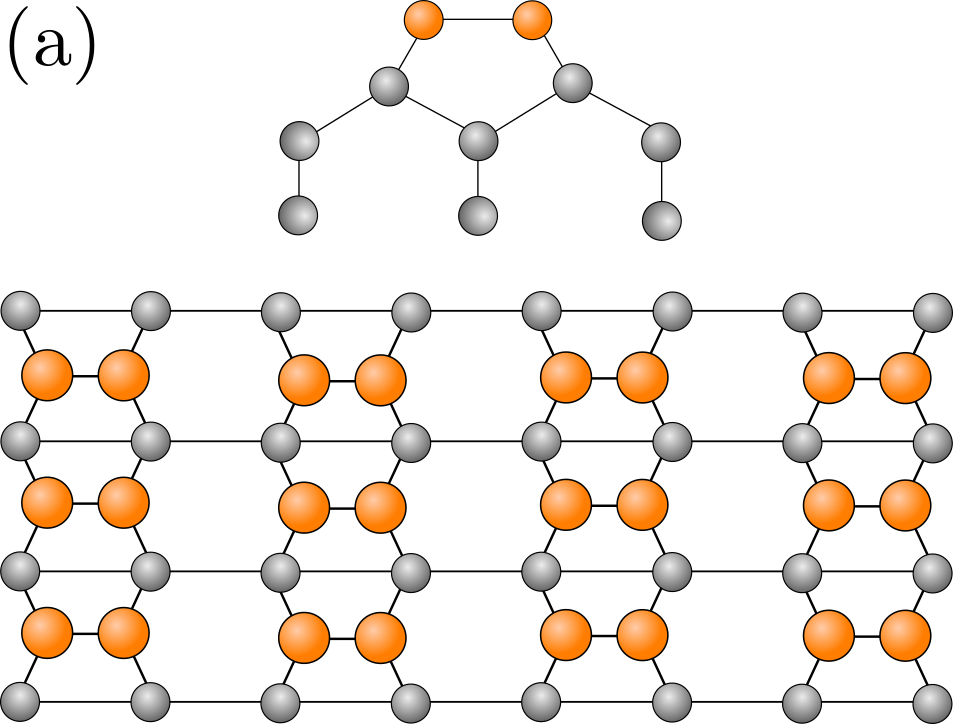
\includegraphics[width=0.8\textwidth]{graphics/p(2x1)-sym.png}
			\label{p(2x1)-symmetric}
		\end{subfigure}
		\begin{subfigure}{0.5\textwidth}
			\centering
			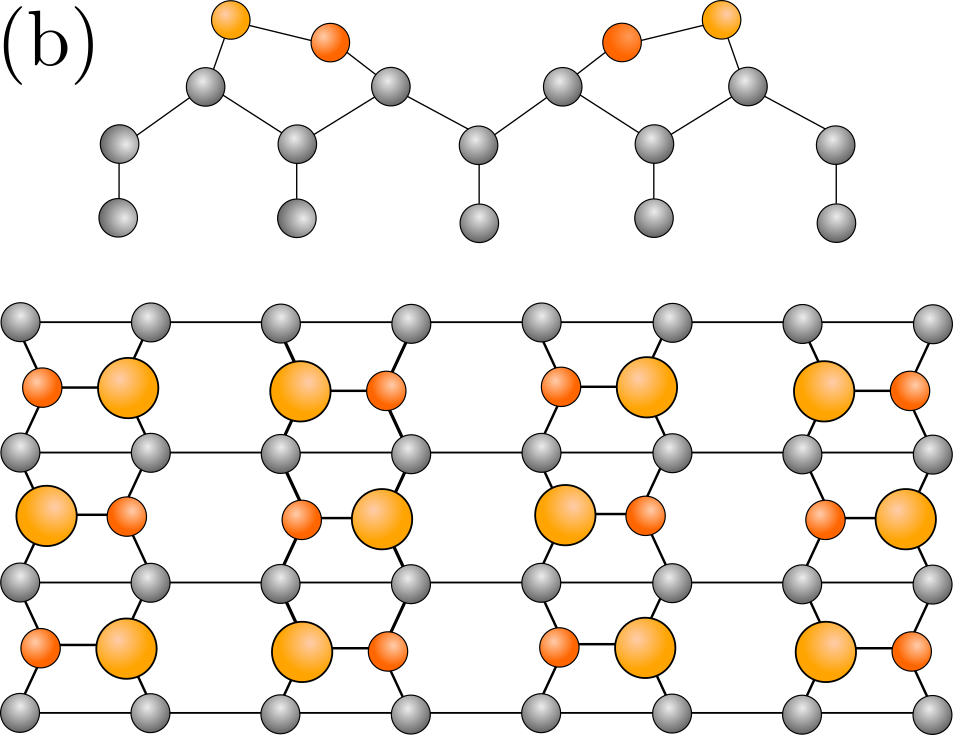
\includegraphics[width=0.8\textwidth]{graphics/c(4x2).png}
			\label{c(4x2)}
		\end{subfigure}
		\caption{ \textbf{(a)}The formation of dimers results in the symmetric $p(2\times1)$ reconstruction and saves a large amount of $1.8~\text{eV}$ per dimer compared to the ideal $p(1\times1)$ structure. \textbf{(b)} The dimers are unstable to vertical buckling. The buckling pattern that was found to have the lowest surface energy is the $c(4\times2)$ reconstruction.}
		\label{Fig::dimer-configs}
	\end{figure}
	\section{Phase Transition of the Si(0,0,1) Surface}
	The Si(001) surface exhibits an order-disorder phase transition from the disordered $p(2\times1)$ phase shown in \autoref{Fig::dimer-configs} (a) to the ordered $c(4\times2)$ reconstruction at a critical temperature of about $T_c \approx 200~\text{K}$ \cite{tabata1987order}. This continuous phase transition will be of central importance in the following discussion. The $p(2\times1)$ structure is short term for the disordered phase since fast flipping of the dimers at a frequency of about $ 10^{-11} \text{ Hz}$ let the system appear to be in the $p(2\times1)$ state at high-temperature measurements. \\
	
	The strong anisotropy leads to long streaks of order along the dimer rows ($\parallel$) and short domains of order across the dimer rows ($\perp$) . Brand et. al \cite{brand2023dimer} found that the ratio of correlation length amplitudes $\xi^+$ is ${\xi_{\parallel}^+}/{\xi_{\perp}^+} \approx 5.2$. The lattice spacing along the dimer rows is $a_\parallel =	3.84~\text{\AA}$, while it is $a_\perp =	2 a_\parallel =	7.68~\text{\AA}$ across. \\
	
	To understand the phase transition of the Si(001) surface we need to have a general knowledge of phase transitions.
	\chapter{Phase Transitions} \label{Chapter::Phase-Transitions}
	
	The term phase transition describes the process of transition between states of a system by changing an external parameter, like pressure $p$ or temperature $T$. Common types are transitions from an unordered to an ordered state after cooling a system below its critical temperature $T_c$ like the transition from paramagnets to ferromagnets. Intuitively the transitions happen as a result of free energy $F =	U - TS$ minimization. At high temperatures entropy $S$ dominates, leading to unordered states, but at low temperatures the impact of the internal energy $U$ takes over. The minimization of $U$ usually leads to a form of ordering dictated by the microscopic Hamiltonian. \\
	
	%A common type of phase transition is order-disorder transitions when the critical temperature $T_c$ of the system is exceeded, like the transition from ferromagnets to paramagnets. Phenomenologically one could say that the driving force behind the phase transition is the minimization of the free energy $F = U - TS $, with internal energy $U$ and entropy $S$. Below the critical temperature, the internal energy U is minimized leading to a form of ordering dictated by the microscopic Hamiltonian.
	\textbf{Mathematical definition:}
	
	Let $N$ denote the number of components, or equivalently the number of lattice sites, and $V$ the volume of the system in question. The \textbf{thermodynamic limit} $N \rightarrow \infty$ and $V \rightarrow \infty$ describes the limit to infinitely large systems while keeping the density $N/V$ constant. For a system dependent on a set of coupling constants $[K]$ the free energy per site $f$ is defined as
	%In the \textbf{thermodynamic limit} (system volume $V \rightarrow \infty$ or number of sites $N \rightarrow \infty$), we can give a mathematical definition of a phase transition. Consider our system to be dependent on a set of coupling constants $[K]$, which for example can be temperature $T$, pressure $p$ or interaction strength $J$. We define the free energy per site as
	\begin{equation}
		f[K] =	\lim\limits_{N \rightarrow \infty} \frac{F[K]}{N} ~.
	\end{equation}
	%If the thermodynamic limit exists,
	With $f$ a precise definition of the phase boundary is possible. The $d$ coupling constants $[K]$ span the so called phase space. In this $d$-dimensional phase space, the free energy density $f$ is analytic almost everywhere except from the possibility of non-analyticities at certain points, lines, planes, etc. up to dimensionality $d-1$. The connected areas of analyticity are called \textbf{phases} and non-analyticitys with dimension $d-1$ are called \textbf{phase boundaries} or \textbf{critical manifolds}. Since $f$ has to be continuous everywhere, the phase boundaries come in two classes:
	\begin{enumerate}
		\item at least one of the first derivatives $\frac{\partial f}{\partial K_i}$ is discontinuous across the phase transition. This case belongs to the \textbf{first-order phase transition}.
		\item all derivatives $\frac{\partial f}{\partial K_i}$ are continuous. This transition is called the \textbf{continuous phase transition}.
	\end{enumerate}
	The phase transition of the silicon surface belongs to the continuous phase transitions. As the thermodynamic limit is never obtained, descriptions using $f$ are not always reliable. Using the correlation length $\xi$, which simply put describes the spatial extent of fluctuations in the system, a criterion for accurate predictions can be given. If the system size $L$ is much greater than the correlation length $\xi \ll L$ the considered system can be expected to behave according to the ideal behavior described by $f$. \\
	%	The free energy density gives reasonable predictions, when the correlation length $\xi$, which is basically the spatial extent of fluctuations in the system, is much smaller than the system size L, so $\xi \ll L$.

	Phase transitions exhibit rich phenomena like the divergence of the correlation length $\xi$ at the critical point. The reason for the universality of this behavior across different systems will be outlined in the next section with the help of renormalization group theory.
	\section{Renormalization Group Considerations} \label{Section::RG}
	The renormalization group (RG) theory is a general framework to study phase transitions and particle physics. It employs scale invariance arguments, meaning the self-similarity characteristics of systems at different length scales, to investigate their properties. In the following basic considerations as well as important results shall be presented briefly. \\
	\begin{figure}[t]
		\centering
		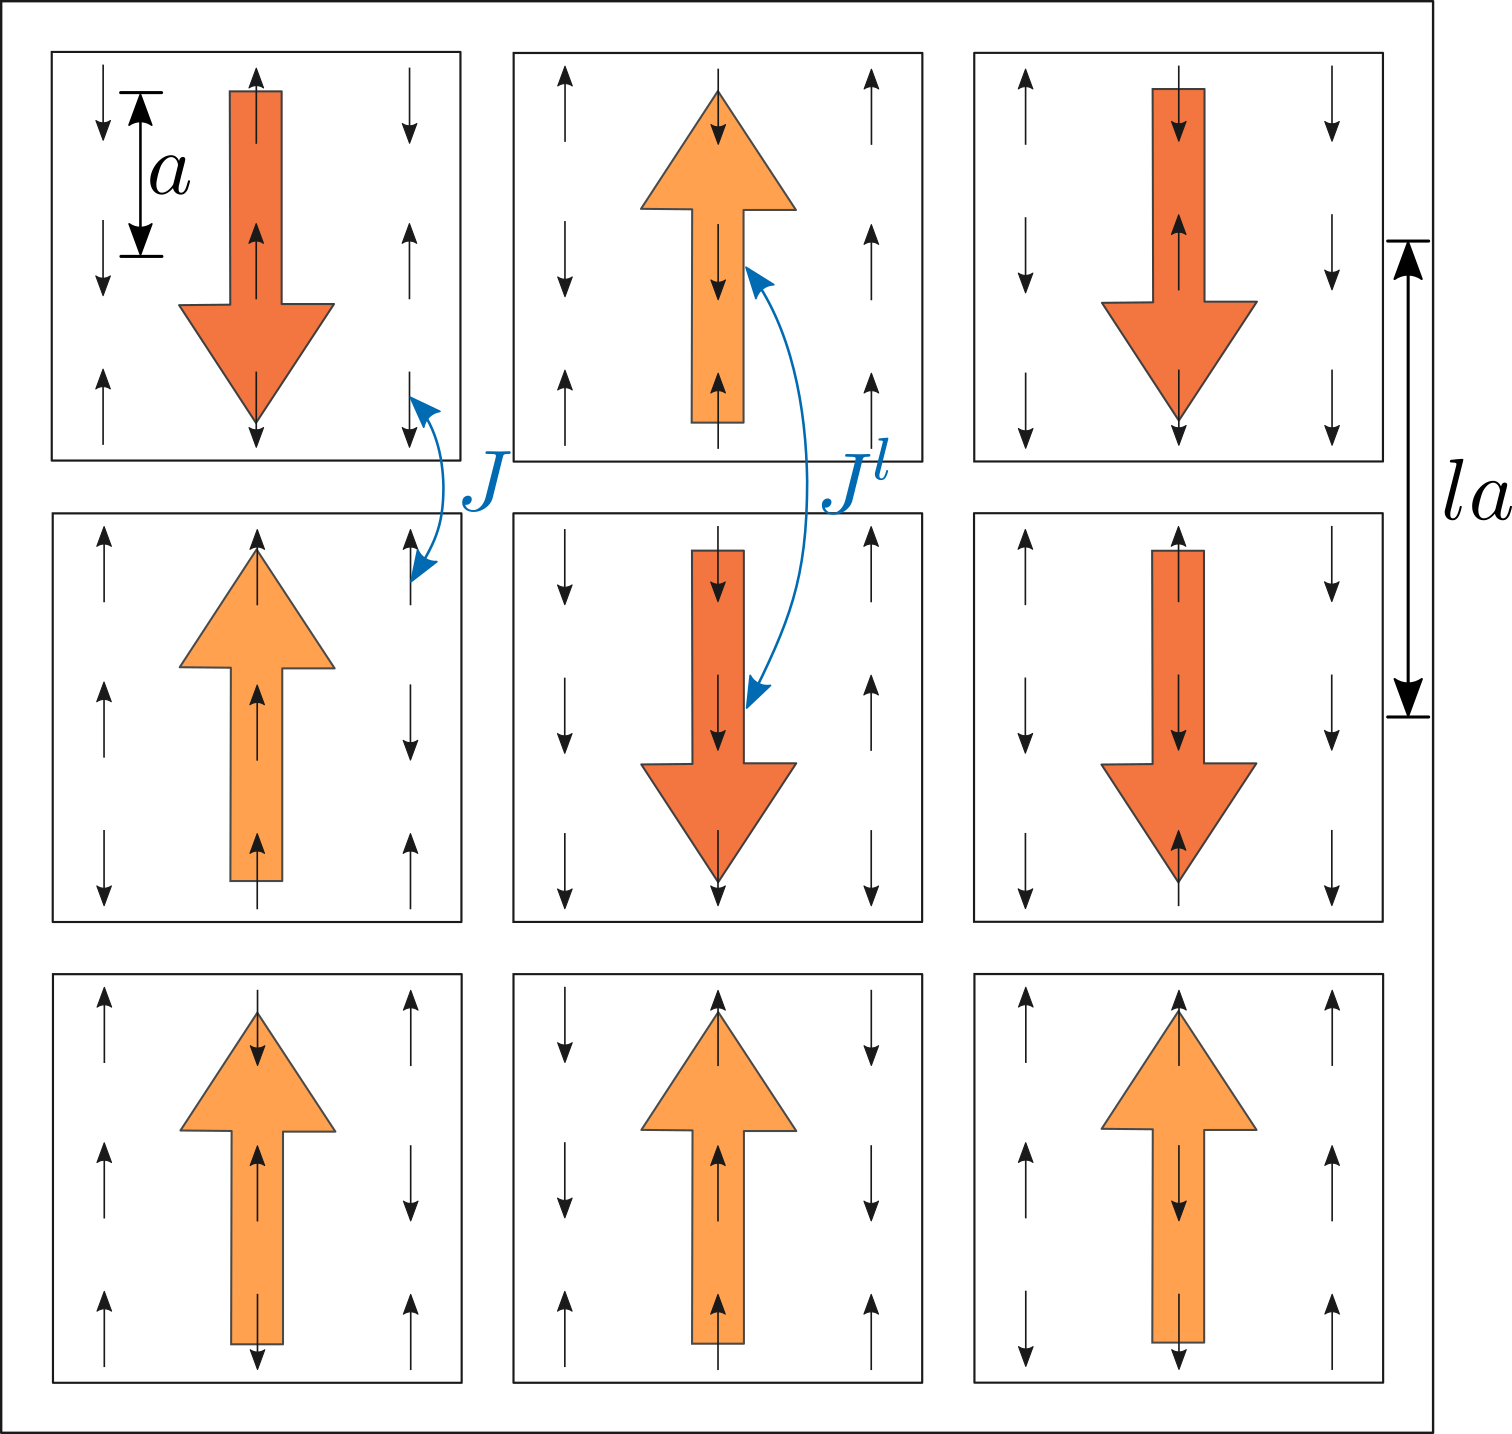
\includegraphics[width=0.7\linewidth]{graphics/RG-Iteration.png}
		\caption{In Kadanoffs block spin picture, $l^2$ Ising-spins are combined to a composite spin that takes on the value of the majority of spins. The block spin is the standard example for a renormalization group transformation. Under the RG transformation, the relevant length scales change from $a$ to $la$ and the coupling strengths from $J$ to $J^l =	R_l(J)$.}
		\label{Fig::RG-Iteration}
	\end{figure}
	
	Consider an infinite two-dimensional $d=2$ lattice with Ising-like spins $s_{mn}$ on each site. The site is denoted by a tuple of indices $(m,n)$. Following Kadanoff \cite{kadanoff1966scaling}, we examine a square of length $l$ in lattice spacing units $a$ and map  their combined $l^2$ spins to a single value $S^l$. This block spin is renormalized to $\pm 1$ by taking on the value of the majority of spins. The obtained $S_{ij}^l$ define a new Ising system, but on a different length scale with a new lattice spacing $la$ like shown in \autoref{Fig::RG-Iteration}. The proposal is that there exists a set of coupling parameters $[K^l]$ defining the interaction of the block spins so that the total free energy stays the same. In terms of the free energy density we can write
	\begin{equation} \label{free-energy-density}
		f[K] =	l^{-2} f[K^l]~,
	\end{equation}
	since the free energy density after the transformation has to increase by a factor $l^2$ as we measure in an $l$-times larger length scale. The same considerations are made for the correlation length, giving
	\begin{equation}
		\xi[K] = l \xi[K^l]~.
	\end{equation}
	Suppose we know how the coupling constants change under an RG transformation $R_l$
	\begin{equation}
		[K^l] =	R_l([K])~.
	\end{equation}
	This is the starting point to comprehend why phase transitions exhibit singular behavior. The idea is that even though the partition function
	\begin{equation}
		Z(\{K\})	= \sum_{\{s\}} e^{- \beta H(\{s\}, \{K\})}
	\end{equation}
	is a sum of exponentials which are analytic in $[K]$, the singularities can arise after an infinite number of RG iterations. Applying multiple RG transformations traces out a trajectory in coupling constant space $[K^{(l_1)}] \rightarrow [K^{(l_2)}]  \rightarrow ... \rightarrow [K^{(l_n)}]$ the \textbf{RG flow}. This trajectory is almost always attracted to fixed points. The behavior of a system near a fixed point is the origin of scaling and lets us extract important information, like the shape of the phase diagram.

	A fixed point of the RG	map satisfies
	\begin{equation}
		[K^{(*)}] =	R_l[K^{(*)}] ~.
	\end{equation}
	At this point the correlation length transforms according to
	\begin{equation}
		\xi[K^{(*)}] =	\xi[K^{(*)}] / l~,
	\end{equation}
	meaning that the correlation length either has to be $0$ or $\infty$. The same is true for the free energy density. In proximity of a fixed point we write the initial coupling constants as
	\begin{equation}
		K_i =	K_i^{(*)} + \delta K_i \qquad \text{and} \qquad K_i^l =	R_l(K_i^{(*)} + \delta K_i) =	K_i^{(*)} + \delta K_i^l~.
	\end{equation}
	The RG Transformation of $K_i$ is in general dependent on all $K$ so that
	\begin{equation}
		K^l_i =	K^l_i[K] =	K^l_i(K_1^{(*)} + \delta K_1, K_2^{(*)} + \delta K_2, ...).
	\end{equation}
	The Taylor expansion of $K_i^l$ around the fixed point $[K^{(*)}]$ yields the linearized RG Transformation
	\begin{equation} \label{linearized-RG}
		K_i^l =	K_i^{(*)} + \sum_j \frac{\partial K_i^l}{\partial K_j} \bigg |_{K_j = K_j^{(*)}} \delta K_j + O((\delta K_j)^2) = K_i^{(*)} + \delta K_i^l + O((\delta K_j)^2) ~.
	\end{equation}
	Omitting terms quadratic in $\delta K_j$ identifies
	\begin{equation}
		\delta K_i^l =	\sum_j \frac{\partial K_i^l}{\partial K_j} \bigg |_{K_j = K_j^{(*)}} \delta K_j~.
	\end{equation}
	We write down the partial derivatives as a matrix
	\begin{equation}
		M^l_{ij} =	\frac{\partial K_i^l}{\partial K_j} \bigg |_{K_j = K_j^{(*)}}~,
	\end{equation}
	and construct an eigenvalue problem
	\begin{equation} \label{ev-problem}
		M^l k^{(\sigma)} =	\lambda^{(\sigma)}_l k^{(\sigma)}~,
	\end{equation}
	where $\sigma$ labels the eigenvalues. Because two consecutive RG Transformations by $l_1$ and $l_2$ have to yield the same result as one  by $l_1l_2$, we know that
	\begin{equation}
		M^{l_1}M^{l_2} =	M^{l_1l_2}~,
	\end{equation}
	implying that
	\begin{equation}
		\lambda_{l_1}^{(\sigma)} \lambda_{l_2}^{(\sigma)} =	\lambda_{l_1l_2}^{(\sigma)} ~.
		\label{ev-equation}
	\end{equation}
	Setting $l_2 = 1$ gives $\lambda_{l_1}^{(\sigma)} \lambda_{1}^{(\sigma)} =	\lambda_{l_1}^{(\sigma)}$ which lets conclude that $\lambda_{1}^{(\sigma)} =	1$. Differentiating \autoref{ev-equation} with respect to $l_2$ yields
	%	\begin{equation}
		%		\begin{split}
			%			\frac{\text{d}}{\text{d}l_2} \left(\lambda_{l_1}^{(\sigma)} \lambda_{l_2}^{(\sigma)}\right) &= 	\frac{\text{d}}{\text{d}l_2} \lambda_{l_1l_2}^{(\sigma)} \\
			%			\lambda_{l_1}^{(\sigma)}  \left(\frac{\text{d}}{\text{d}l_2} \lambda_{l_2}^{(\sigma)}\right) +  			  \left( \frac{\text{d}}{\text{d}l_2} \lambda_{l_1}^{(\sigma)}\right) \lambda_{l_2}^{(\sigma)} &= l_1 \frac{\text{d}}{\text{d}(l_1l_2)} \lambda_{l_1l_2}^{(\sigma)} \\
			%			\left(\frac{\text{d}}{\text{d}l_2} \lambda_{l_2}^{(\sigma)}\right) \lambda_{l_1}^{(\sigma)}   &= l_1 \frac{\text{d}}{\text{d}(l_1l_2)} \lambda_{l_1l_2}^{(\sigma)}	~.
			%		\end{split}
		%	\end{equation}
	\begin{equation}
		\frac{\text{d}}{\text{d}l_2} \left(\lambda_{l_1}^{(\sigma)} \lambda_{l_2}^{(\sigma)}\right) = \lambda_{l_1}^{(\sigma)}  \left(\frac{\text{d}}{\text{d}l_2} \lambda_{l_2}^{(\sigma)}\right) +  			  \left( \frac{\text{d}}{\text{d}l_2} \lambda_{l_1}^{(\sigma)}\right) \lambda_{l_2}^{(\sigma)} 	= \left(\frac{\text{d}}{\text{d}l_2} \lambda_{l_2}^{(\sigma)}\right) \lambda_{l_1}^{(\sigma)}
	\end{equation}
	for the left hand side and
	\begin{equation}
		\frac{\text{d}}{\text{d}l_2} \lambda_{l_1l_2}^{(\sigma)} =	\frac{\text{d}}{\text{d}(l_2 l_1)} \lambda_{l_1l_2}^{(\sigma)} \frac{\partial}{\partial l_2} (l_1 l_2) =	l_1 \frac{\text{d}}{\text{d}(l_1l_2)} \lambda_{l_1l_2}^{(\sigma)}
	\end{equation}
	for the right hand side. By setting $l_2 =	1$ the differential equation
	\begin{equation}\label{RG-diff}
		\frac{\text{d}}{\text{d}l_2} \lambda_{l_2}^{(\sigma)} \bigg |_{l_2 =	1} \lambda_{l_1}^{(\sigma)}  = y_\sigma \lambda_{l_1}^{(\sigma)} = l_1 \frac{\text{d}}{\text{d}l_1} \lambda_{l_1}^{(\sigma)}
		%\quad \Rightarrow \quad \frac{\text{d}}{\text{d}l_1} \lambda_{l_1}^{(\sigma)} =	\frac{y_\sigma}{l_1} \lambda_{l_1}^{(\sigma)} ~.
	\end{equation}
	with
	\begin{equation}
		y_\sigma = \frac{\text{d}}{\text{d}l_2} \lambda_{l_2}^{(\sigma)} \bigg |_{l_2 =	1}
	\end{equation}
	is obtained.
	A solution to \textsf{\autoref{RG-diff}} is
	\begin{equation} \label{ev-form}
		\lambda_l^{(\sigma)} = l^{y_\sigma}~,
	\end{equation}
	with $y_\sigma$ being independent of $l$. This is an important result on the way to show the origin of scaling. The $k^{(\sigma)}$ are vectors in the coupling constant space, so \autoref{ev-problem} indicates that some $\delta K_i$ grow and some shrink when applying RG transformations, depending on the eigenvalue $\lambda_l^{(\sigma)}$. Three cases are distinguished:
	\begin{enumerate}
		\item \textbf{Relevant} directions and eigenvalues:	$|\lambda_l^{(\sigma)}| > 1$, meaning that $y_\sigma > 0$ and $\delta K$ in direction of $k^{(\sigma)}$ grow.
		\item \textbf{Irrelevant} directions and eigenvalues:	$|\lambda_l^{(\sigma)}| < 1$, meaning that $y_\sigma < 0$ and $\delta K$ in direction of $k^{(\sigma)}$ shrink.
		\item \textbf{Marginal} directions and eigenvalues:	$|\lambda_l^{(\sigma)}| = 1$, meaning that $y_\sigma = 0$ and $\delta K$ in direction of $k^{(\sigma)}$ do not change.
	\end{enumerate}
	After many iterations, only the relevant eigenvalues will be important, as shrinking $\delta K_i$ won't impact the RG flow significantly. If we differ from the fixed point in a relevant direction, the differences to the fixed point will become larger and the RG transformation flow will move away from the fixed point. Deviations in irrelevant direction will flow into the fixed point. \\
	
	A simplified understanding can be achieved for a system satisfying
	\begin{equation}
		\frac{\partial K_i^l}{\partial K_j} \bigg |_{K_j = K_j^{(*)}} = \delta_{ij} \frac{\partial K_j^l}{\partial K_j} \bigg |_{K_j = K_j^{(*)}}~,
	\end{equation}
	so that $M^l_{ij}$ becomes diagonal and the eigendirections $k^{(\sigma)}$ point directly along the axes $e^{K_i}$ of the phase space defined by $K$. If the eigenvalue $\lambda_l^{(\sigma)}$ to $k^{(\sigma)}$, parallel to $e^{K_i}$, is larger than one, the coupling $K_i$ will grow. In this case $K_i$ would be a relevant coupling constant. \\
	
	Consider a system with only one coupling constant, in this case the temperature, and choose $T$ in the vicinity of a fixed point $T^{(*)}$. Apply a RG transformation to $T$ and consider the difference
	\begin{equation} \label{temp-difference}
		T^l - T^{(*)} =	R_l(T) - T^{(*)}~.
	\end{equation}
	Using \autoref{linearized-RG} we can rewrite
	\begin{equation}
		R_l(T) =	T^{(*)} + \delta T^l =	T^{(*)} + \frac{\partial T^l}{\partial T} \bigg |_{T =	T^{(*)}} \delta T =	T^{(*)} + \lambda_l \delta T~,
	\end{equation}
	since $M^l$ has only one component and $\delta T$ is therefore automatically in eigenvector direction. \autoref{temp-difference} then becomes
	\def\equationautorefname{Eq.}
	\begin{equation} \label{coupling-constant-ev-scaling}
		\varepsilon^{(l)} =	\lambda_l \varepsilon \overset{\text{\autoref{ev-form}}}{=} \varepsilon l^{y_\varepsilon}~,
	\end{equation}\def\equationautorefname{equation}
	in terms of the \textbf{reduced temperature} $ \varepsilon =	\frac{T - T^{(*)}}{T^{(*)}}$. After $n$ RG iterations this gives
	\begin{equation}
		\varepsilon^{(nl)} = \left( l^{y_\varepsilon}	\right)^n \varepsilon~.
	\end{equation}
	Now consider again how the correlation length transforms after $n$ RG transformations
	\begin{equation} \label{xi-behavior}
		\xi(\varepsilon) =	l^n \xi(\varepsilon^{nl}) =	l^n \xi( l^{ny_\varepsilon} \varepsilon)~.
	\end{equation}
	Substituting $\tau =	l^{ny_\varepsilon} \varepsilon$ into \autoref{xi-behavior} yields
	\begin{equation} \label{Eq::RG-xi-scaling}
		\xi(\varepsilon) =	\tau^{1 / y_\varepsilon} \varepsilon^{-1/ y_\varepsilon} \xi(\tau)~,
	\end{equation}
	showing that the correlation length diverges as $\varepsilon \rightarrow 0$. This is the origin of scaling and universality! Note that knowledge of a valid RG transformation $R_l$ directly provides knowledge of $y_\varepsilon$ via
	\begin{equation}
		y_\varepsilon =	\frac{1}{l} \ln \left(\frac{\partial R_l (T)}{\partial T} \bigg|_{T^{(*)}}\right)~.
	\end{equation}
	\section{Universality and Static Scaling} \label{Section::Universality}
	The last section traced the origin of universality and scaling in phase transitions. This section will deal with the term universality and its implications in more detail. \\
	
	Scaling laws like \autoref{Eq::RG-xi-scaling} can be derived for different system quantities. In the context of phase transitions, \textbf{static scaling} means the power law dependence of a system quantity \textbf{in equilibrium}, like the correlation length $\xi$, on a coupling parameter, like the temperature $T$. The exponent of this power law is called the \textbf{critical exponent}. Some important scaling relations are shown in \autoref{Table::Scaling-Laws}. Comparing the scaling law of $\xi$ with \autoref{Eq::RG-xi-scaling} identifies
	\begin{equation}
		\frac{1}{y_\varepsilon} = \nu ~.
	\end{equation}
	%	\begin{itemize}
		%		\item the specific heat $\boldsymbol{C_H}$: $T_c C_H \approx A^{\pm} |\varepsilon|^{-\alpha}$,
		%		\item the order parameter $\boldsymbol{\Psi}$ or $\boldsymbol{M}$: $|M| \approx B |\varepsilon|^{-\beta}$,
		%		\item the susceptibility $\boldsymbol{\chi}$: $\chi \approx C^{\pm} |\varepsilon|^{-\gamma}$,
		%		\item and the correlation length $\boldsymbol{\xi}$ : $\xi \approx f^{\pm} |\varepsilon|^{-\nu}$.
		%	\end{itemize}
	\begin{table}[h]
		\centering
		\caption{Some important scaling laws are summarized in the notation of \cite{pelissetto2002critical}. The universal critical exponents $\alpha, \beta,$ etc. are the same above and below the phase transition. In contrary, the nonuniversal critical amplitudes may differ at different sides of the critical point. Hence, they are labeled with a superscript $\pm$. The dimensionality is denoted by $d$.}
		\begin{tabular}{l c l}
			\toprule
			Name  & $\quad$ Symbol $\quad$ & Scaling \\
			\midrule
			specific heat & $C_H$ & $T_c C_H \approx A^{\pm} |\varepsilon|^{-\alpha}$ \\
			order parameter & $\Psi, M$ & $|M| \approx B |\varepsilon|^{-\beta}$ \\
			susceptibility & $\chi$ & $\chi \approx C^{\pm} |\varepsilon|^{-\gamma}$ \\
			correlation length & $\xi$ & $\xi \approx f^{\pm} |\varepsilon|^{-\nu}$ \\
			two-point correlation function & $C(\vec{r})$& $C(\vec{r}) \propto |\vec{r}|^{- d + 2 - \eta}$ \\
			\bottomrule
		\end{tabular}
		\label{Table::Scaling-Laws}
	\end{table}
	The prefactors of the power laws are called the \textbf{critical amplitudes} and $\nu, \alpha, $ etc. are the mentioned critical exponents. The superscript $\pm$ denotes whether the phase transition is approached from below $(-)$ or above $(+)$ the critical temperature $T_c$. The critical exponents are the same on both sides of the transition, but the amplitudes vary. \\
	
	These scaling laws are only valid in the thermodynamic limit for $\varepsilon \rightarrow 0$ as the derivation in \autoref{Section::RG} assumed that the system is in the vicinity of a critical point. Otherwise they exhibit \textbf{corrections to scaling} that result out of irrelevant and marginal eigenvalues of the RG transformations as well as \textbf{finite-size} corrections. \\
	
	Systems that share the same set of critical exponents belong to the same \textbf{universality class}. \autoref{Section::RG} showed that the exponents can be calculated solely from the RG transformation which suggests that systems with similar transformations exhibit similar critical behavior. Indeed it is found that the universality class of a system only depends on
	\begin{itemize}
		\item the \textbf{symmetry group} of the system Hamiltonian,
		\item the \textbf{dimensionality} of the problem,
		\item and whether the \textbf{interaction} between the components is \textbf{short-ranged}.
	\end{itemize}
	In contrast to the critical exponents, the critical amplitudes are not universal, but their ratios, for example $f^+/f^-$, are.\\
	
	The concept of universality is very useful to investigate real systems at the critical point. As a result of scale invariance and self similarity, the microscopic dynamics of a system become irrelevant at $\varepsilon =	0$. Its behavior can then be approximated by a simplified, in the best case exactly solvable, model. \\
	
	The extraction of critical exponents is notoriously difficult for various reasons, one being the inaccessibility of the thermodynamic limit, another \textbf{critical slowing down} (see \autoref{Section::Dynamic-Scaling}). The following section will explain the mentioned finite size corrections to static scaling and illustrate how they can be used to analyze critical exponents.
	\section{Finite-size Scaling and Critical Exponent Extraction} \label{Section::FSS}
	The system size $L$ transforms after RG transformation according to
	\begin{equation}
		R_l(L) =	L^{(l)} =	L /	l ~,
	\end{equation}
	analogous to the correlation length. Extending the transformation of the free energy density of \autoref{free-energy-density} by a dependence of the system size yields
	%	Recall how the free energy density \autoref{free-energy-density} transforms and that it depends on the system size $L = l L^{(l)}$:
	\begin{equation}\label{FSS-free-energy-scaling}
		f\left([K], L^{-1}\right) =	l^{-2} f\left([K^{(l)}], {L^{(l)}}^{-1}\right) = l^{-2} f\left([K^{(l)}], l{L}^{-1}\right)	 ~,
	\end{equation}
	the \textbf{finite-size scaling} (FSS) of $f$.
	Let $K_1 =	\varepsilon$ be the reduced temperature. Close to the critical point \autoref{coupling-constant-ev-scaling} can be used to write \autoref{FSS-free-energy-scaling} in terms of eigenvalues
	\begin{equation}
		f\left(\varepsilon, K_2, ..., L^{-1}\right) = l^{-2} f\left(\varepsilon l^{y_\varepsilon}, K_2 l^{y_2}, ..., l{L}^{-1}\right)	 ~.
	\end{equation}
	The system size behaves like a relevant coupling constant with an eigenvalue of
	\begin{equation}
		\lambda_L =	1~, \qquad \text{implying that} \qquad y_L =	1 ~.
	\end{equation}
	This means that the system size has to be tuned to criticality for the phase transition to occur. Like $\varepsilon$, the inverse system size has to be set zero $L^{-1} =	0$ which is equivalent to taking the thermodynamic limit. As a result, real, finite systems deviate from the behavior that scaling laws dictate. The actual correlation length cannot outgrow the system size $\xi_L \leq L$ and so the divergence of $\xi$ is rounded at the phase transition. Additionally,  the peak of $\xi_L(T)$ is shifted \cite{guton1983phase} (to a lower critical temperature?). The ideal behavior of $\xi$ is compared to the behavior of a finite system in  \autoref{xi-divergence-FS}. \\
	
	\begin{figure}[htp]
		\centering
		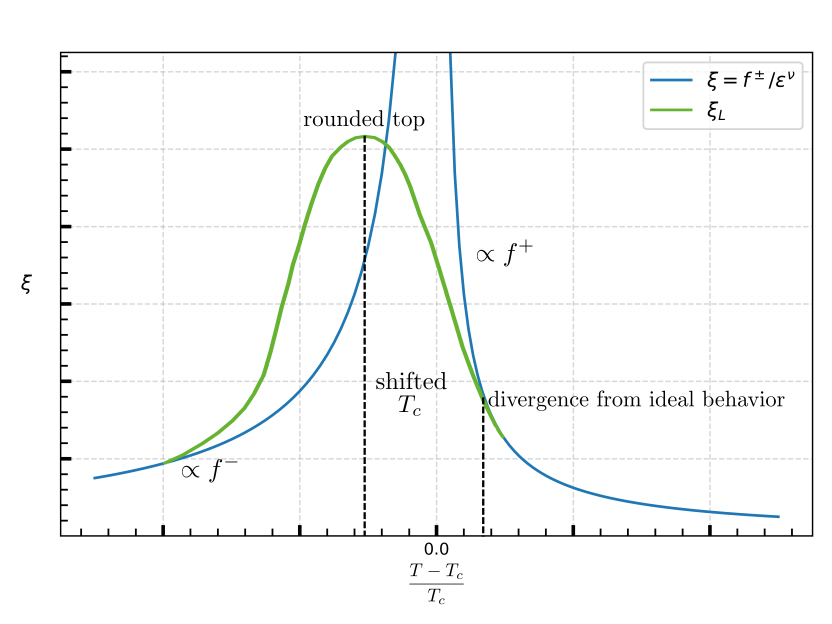
\includegraphics[width=0.7\linewidth]{graphics/xi-divergence4.png}
		\caption{The equilibrium correlation length $\xi$ is shown versus the reduced critical temperature. In the thermodynamic limit, $\xi$ diverges at the critical point according to a power law, as depicted by the blue line. For finite systems, the singularity of $\xi$ appears rounded as shown by the green curve. The peak position is shifted to an effective critical temperature.}
		\label{xi-divergence-FS}
	\end{figure}
	Now consider \autoref{xi-behavior} extended by $L$-dependence reading
	\begin{equation}
		\xi(\varepsilon, L^{-1}) =	l \xi (\varepsilon l^{y_\varepsilon}, l L^{-1}) = \varepsilon^{-\nu} F_\xi (L^{-1} \varepsilon^{-\nu})~,
	\end{equation}
	with $F_\xi$ as in \autoref{Eq::RG-xi-scaling}. Introducing a new scaling function $F' =	(L \varepsilon^\nu)^{-1} F_\xi$ yields
	\begin{equation}
		\xi(\varepsilon, L^{-1}) = \varepsilon^{-\nu} (L\varepsilon^\nu) F' (L \varepsilon^{\nu}) =	L	F'(L \varepsilon^\nu)~.
	\end{equation}
	In the limit $L \rightarrow \infty$ and close to $\varepsilon =	0$, $\xi$ has to scale like $\xi(\varepsilon, 0) \propto \varepsilon^{-\nu}$ implying that
	\begin{equation}
		\lim_{L \rightarrow \infty} \lim_{\varepsilon \rightarrow 0} F'(L \varepsilon^\nu) \propto (L \varepsilon^\nu)^{-1}~.
	\end{equation}
	The correlation length is capped for finite $L$ so that at the critical point $\xi(0, L^{-1}) \propto L$. For $F'$ this means
	\begin{equation}
		\lim_{\varepsilon \rightarrow 0} F'(L\varepsilon^\nu) \propto \text{const.}~,
	\end{equation}
	showing that the scaling function does not diverge. Therefore a Taylor expansion around $\varepsilon =	0$ is reasonable and gives
	\begin{equation} \label{Equation::FSS-Scaling-L/xi}
		\frac{L}{\xi(\varepsilon, L^{-1})} =	A + B \varepsilon L^{1/\nu} + O(\varepsilon^2)~. 
	\end{equation}
	This equation is an important result since it can be used to calculate two central quantities. Firstly, curves of $L/\xi(\varepsilon, L^{-1})$ for different $L$ intersect at the critical point $\varepsilon = 0$. Hence, by determining this intersection one can extract the critical temperature $T_c$, which is usually not known a priori. Secondly by computing the gradient
	\begin{equation}
		\frac{\partial}{\partial \varepsilon} \left(\frac{L}{\xi(\varepsilon, L^{-1})}\right) =	B L^{1/\nu}
	\end{equation}
	for various $L$, one can determine the critical exponent $\nu$. This method is easier than, for example, trying to fit to the original scaling law \autoref{Eq::RG-xi-scaling} because of the reasons mentioned at the end of \autoref{Section::Universality}.
	\subsection{Binder Cumulant} \label{Sec::Binder-Cumulant}
	FFS scaling laws like \autoref{Equation::FSS-Scaling-L/xi} can be derived for any thermodynamic quantity \cite{pelissetto2002critical, blote1995ising}. The Binder cumulant $U_L$, introduced by K. Binder in \cite{binder1981finite}, is frequently used to investigate simulations. It is defined as
	\begin{equation} \label{Eq::Def-Binder-Cum}
		U_L =	\frac{\langle M_L^4 \rangle}{\langle M_L^2 \rangle^2}~,
	\end{equation}
	with $M_L$ being the order parameter of a system of size $L$. The ensemble average $\left\langle~\cdot~\right \rangle$ denotes the mean of infinitely many system realizations. Its finite size scaling is analogous to \autoref{Equation::FSS-Scaling-L/xi} given by
	\begin{equation}
		U_L =	U^* + U \varepsilon L^{1/\nu} \left(1 + W L^{-\omega} + ...\right)~,
	\end{equation}
	including corrections resulting out of the largest irrelevant eigenvalue $1/|y_1| =	\omega $.
	To extract the critical exponent $\nu$ a linear fit to
	\begin{equation} \label{Eq::FSS-dU_dT}
		\ln \left(\frac{\partial U_L}{\partial \varepsilon}\right) \approx	\ln \left(U L^{1/\nu} \right) =	\ln (U) + \frac{1}{\nu} \ln (L) ~.
	\end{equation}
	is performed.
	The Binder cumulant has a value of $U_L=1$ far below the phase transition, approaches $U_L =	3$ above the phase transition and exhibits the intersection in between at $U_L =	U^*$. It is generally easy to compute and extract.
	\section{Dynamic Scaling and the Kibble-Zurek Mechanism} \label{Section::Dynamic-Scaling}
	\subsection{The Relaxation Time $\tau$ and the Critical Exponent $z$}
	With the Binder cumulant we acquired a way to extract the static scaling exponent $\nu$. Aside static scaling, \textbf{dynamic critical phenomena} are of central importance to describe phase transitions. Dynamic scaling describes how much time fluctuations in systems take to equilibrate. This time is called the  \textbf{relaxation time} $\tau_k$ and it is usually specified for different lengthscales with the wavenumber $k$. The zero wavenumber relaxation time $\tau_0 =	\tau$ quantifies relaxation on the largest lengthscales. Its scaling \cite{hohenberg1977theory}
	\begin{equation}
		\tau =	\tau_\xi \xi(\varepsilon)^z
	\end{equation}
	defines a new \textbf{dynamic critical exponent} z. (TODO RG explanation for this scaling?). \\
	
	Plugging in the known scaling of $\xi(\varepsilon)$ from \autoref{Section::Universality} yields
	\begin{equation}
		\tau = \tau_\xi \xi(\varepsilon)^z =\tau_\xi	\left(f^{\pm} |\varepsilon|^{-\nu}\right)^z :=	\tau_\varepsilon |\varepsilon|^{-\nu z} ~.
	\end{equation}
	As the correlation length diverges, so does the relaxation time. Interpreting $\xi$ as a characteristic length at which system components are still influenced by each other gives an intuitive explanation for this divergence. The maximum speed for the propagation of interactions in the system is the respective speed of sound. Even the speed of sound would need an infinite amount of time to cover an infinite distance. In practice the propagation will take much more time. This is the in \autoref{Section::Universality} mentioned phenomenon of critical slowing down. As a system approaches $\varepsilon \rightarrow 0$, it takes longer and longer to equilibrate. It then becomes a computational challenge to let large systems equilibrate. But since static scaling laws describe quantities in equilibrium and are only valid in the thermodynamic limit for $\varepsilon \rightarrow 0$, large, critical systems have to be considered.  This dilemma was partially solved by the finite size techniques of \autoref{Section::FSS}. \\
	
	As well as its complementary static phenomenon does the dynamic scaling exhibit universality. The static and dynamic universality classes are not independent, but the dynamic ones form subgroups of the static universality classes. Besides the usual indicators described in \autoref{Section::Universality}, the conservation laws that are fulfilled by the system, as well as Poisson-bracket relations between the order parameter and the conserved densities are decisive for the respective universality class. The important anisotropic Ising model is part of Model A(?) as specified by Hohenberg and Halperin \cite{hohenberg1977theory}. Its dynamic critical exponent can be expressed in terms of
	\begin{equation}
		z =	2 + c \eta ~,
	\end{equation}
	with $\eta$ as in \autoref{Table::Scaling-Laws} and $c$ a constant to be determined.
	\subsection{Quenches and the Freezeout of Domains}
	Systems like the Si(001) surface that exhibit order-disorder phase transitions usually have multiple possible orderings in the low temperature state. Boundaries between domains of different order, also called domain walls, are stable topological defects. The \textbf{Kibble-Zurek mechanism} (KZM) \cite{kibble1976topology, zurek1985cosmological, zurek1996cosmological} describes the final density of topological defects after driving a system through its phase transition. It directly relates the correlation length to the static and dynamic critical exponents $\nu$ and $z$ through a scaling law that has been verified in numerous experiments \cite{ruutu1996vortex, ulm2013observation, pyka2013topological}. The KZM shall be a central point of the upcoming investigations and will be explained in the following. \\
	
	We will solely consider linear quenches, concretely the cooldown of a system linear in time $t$. The speed of cooling is characterized by the \textbf{quench timescale} $\tau_Q$ defined by
	\begin{equation} \label{Eq::Linear-Quench}
		\varepsilon(t) =	\frac{t}{\tau_Q}~.
	\end{equation}
	For slow quenches sufficiently far away from the critical point, the system will evolve adiabatically, meaning that thermodynamic quantities like $\xi$ assume their equilibrium values. As the system approaches the phase transition at $t=0$, the derivative
	\begin{equation}
		\frac{\partial}{\partial t} \xi(\varepsilon(t)) =	- \nu f^{\pm} \frac{(\tau_Q)^\nu}{t^{-(\nu + 1)}}
	\end{equation}
	diverges and at some point will eventually outgrow the reaction capability of the system. The actual correlation length will diverge from its equilibrium behavior like shown in \autoref{Fig::Freezeout}. The timepoint $\hat{t}$ of divergence from the equilibrium behavior is called the \textbf{freezeout} since the current state of the system effectively becomes frozen in comparison with the equilibrium values. The KZM states that the freezeout roughly happens at
	% when the current relaxation time $\tau$ equals the time until the crossing of the critical point $\hat{t}$, defining
	\begin{equation}
		\tau(\hat{t}) = \hat{t}~,
	\end{equation}
	so as soon as $\tau$ exceeds the time that is left until the critical point is crossed.
	\begin{figure}[t!]
		\centering
		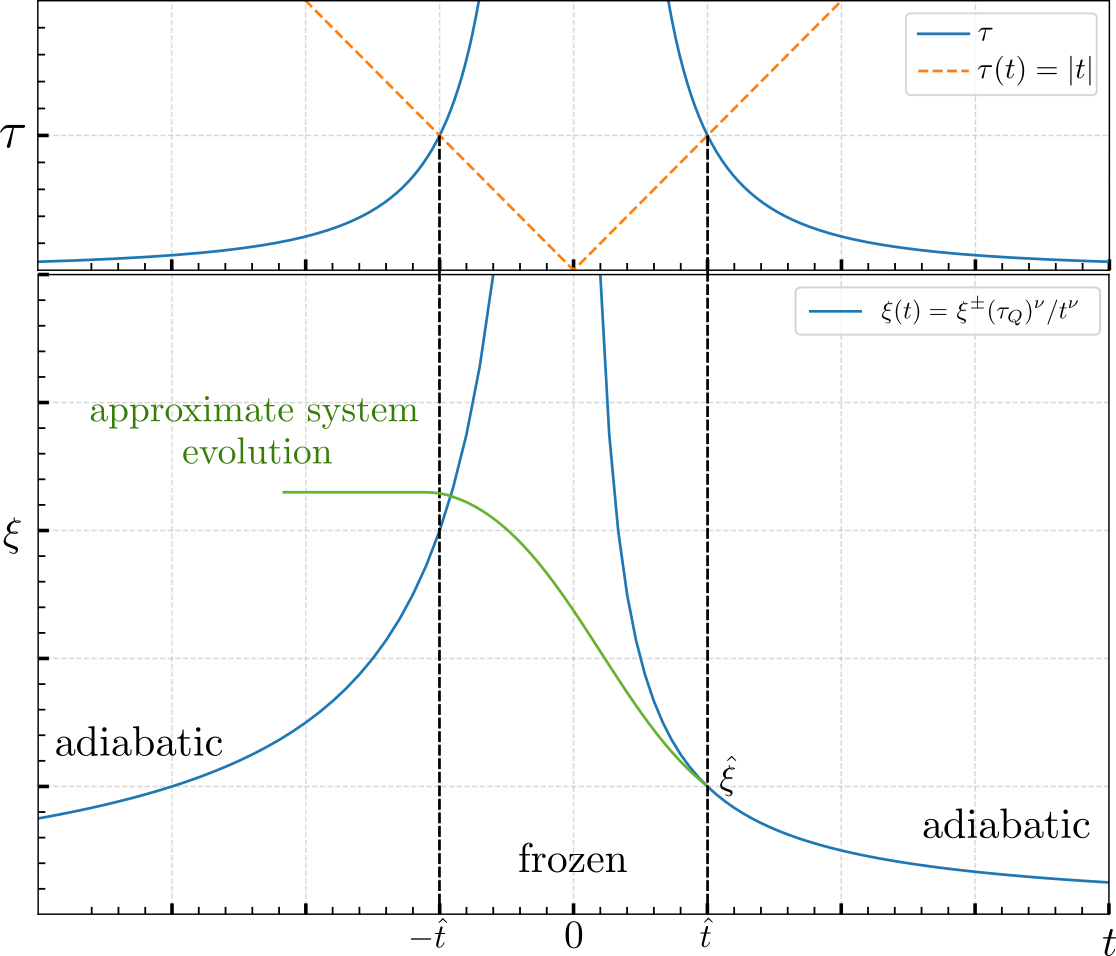
\includegraphics[width=0.7\linewidth]{graphics/KZM-divergences.png}
		\caption{In the top plot the divergence of the relaxation time $\tau$, i.e. the critical slowing down, is shown in blue versus the time $t$ during a linear quench. The freezeout of the current state happens roughly at $\tau(\hat{t}) =	\hat{t}$, visualized by the intersection with the dotted orange line. In the bottom plot the divergence of the equilibrium $\xi$ on the quench time is shown. Before $\hat{t}$ a quenched system evolves approximately adiabatic, following the blue line. After the freezeout, the actual correlation diverges from the equilibrium behavior, shown by the green line. Note that in this parameterization, a cooling quench runs from $t > 0$ to $t < 0$. The frozen domain walls are topologically stable in time.}
		\label{Fig::Freezeout}
	\end{figure}
	The system quantities after the quench will be directly related to their equilibrium values at $\hat{t}$. Combining
	\begin{equation}
		\hat{t} =	\varepsilon(\hat{t}) \tau_Q \qquad \text{and} \qquad  \hat{t} =	\tau(\hat{t}) = \tau(\varepsilon(\hat{t})) =	\tau_\varepsilon \big | \varepsilon(\hat{t}) \big |^{-\nu z}
	\end{equation}
	yields the reduced temperature at $\hat{t}$
	\begin{equation}
		\big|\varepsilon (\hat{t}) \big| =	\left(\frac{\tau_\varepsilon}{\tau_Q} \right)^{\frac{1}{1 + \nu z}} ~.
	\end{equation}
	For the scaling of $\xi$ this means
	\begin{equation} \label{Eq::KZM-scaling}
		\xi \propto \hat{\xi} := \xi(\varepsilon(\hat{t})) =	\xi_0 / |\varepsilon(\hat{t})|^{\nu} =	\xi_0 \bigg| \frac{\tau_Q}{\tau_\varepsilon} \bigg |^{\frac{\nu}{1 + \nu z}} ~,
	\end{equation}
	so the frozen value of the correlation length scales with the quench timescale like $\hat{\xi} \propto \tau_Q^{\frac{\nu}{1 + \nu z}}$~.
	The freezeout of the correlation length implies domains of order with an extent proportional $\hat{\xi}^2$. The domain walls separating ordered areas may have influences on different properties of the surface, including conductivity, an important quantity for the semiconductor industry. Knowledge of how the defect density on the surface behaves might help to prepare ideal silicon surfaces. \\
	
	It is important to note that the KZM is a statistical phenomenon and will only be able to predict how the frozen correlation lengths will behave on average for many quenches or very large systems. In general the freezeout correlation length $\hat{\xi}$ as well as the final correlation length will naturally differ from the predicted behavior, at least locally.
	\chapter{Simulating Dynamics} \label{Chapter::Simulating-Dynamics}
	While most numerical studies of phase transitions rely on monte carlo techniques \cite{rastelli2004monte, ferrenberg1991critical, hasenbusch2005two}, this work, inspired by Laguana and Zurek \cite{laguna1997density}, focuses on the use of \textbf{stochastic differential equations}. Their mathematical basics and a derivation of a Langevin equation for our case  will be outlined in the following.
	\section{Stochastic Differential Equations and the Langevin Equation}
	Put simply, stochastic differential equations (SDEs) are the stochastic generalizations of common differential equations like
	\begin{equation} \label{Eq::diff-eq}
		y(t + dt) =	y(t) + A(y(t), t) dt ~,
	\end{equation}
	where $dt$ denotes an infinitesimal time interval. 	\autoref{Eq::diff-eq} describes a \textbf{continuous, memoryless, deterministic} process. For every timepoint $t + dt$ one can predict the value $y(t+dt)$ knowing the values $y(t)$ and $dt$. SDEs describe continuous, memoryless \textbf{stochastic} processes also called continuous \textbf{markov processes}. For every timepoint we can assign definite probabilities to all $y(t + dt)$. These properties impose relatively strict limitations on a generalization of \autoref{Eq::diff-eq}. It turns out, that the generalization must be of the form \cite{gillespie1996mathematics}
	\begin{equation} \label{Eq::std-langevin-eq}
		y(t + dt) =	y(t) + A(y(t), t) dt + D^{1/2} \left(y(t), t\right) n(t) (dt)^{1/2}~.
	\end{equation}
	The random number $n(t)$ is a sample value of a normal distribution around zero with standard deviation one $\mathcal{N}(0,1)$. \autoref{Eq::std-langevin-eq} is called the standard form \textbf{Langevin equation} and it represents an update formula for the continuous markov process. To obtain the widely used \textbf{differential }or \textbf{white noise }form of the Langevin equation, we define the \textbf{Gaussian white noise process} $\Gamma(t)$ by
	\begin{equation}
		\Gamma(t) :=	\lim\limits_{dt \rightarrow 0} \mathcal{N}(0, 1/dt) \equiv \lim\limits_{dt \rightarrow 0} \frac{n(t)}{(dt)^{1/2}}.
	\end{equation}
	It satisfies
		\begin{equation}
		\left \langle \Gamma(t) \right \rangle = 0 \qquad \text{and} \qquad  			\left \langle \Gamma(t) \Gamma(t + t')\right \rangle =	\delta(t') ~.
	\end{equation}
	Rearranging \autoref{Eq::std-langevin-eq} to
	\begin{equation}
		\frac{y(t + dt) - y(t)}{dt} =	A(y(t), t) + D^{1/2} (y(t), t) \frac{n(t)}{(dt)^{1/2}} ~,
	\end{equation}
	and taking the limit $dt \rightarrow 0$ leads to the differential form
	\begin{equation} \label{Eq::Differential-Langevin-eq}
		\frac{d}{dt} y(t) =	A(y(t), t) + D^{1/2}(y(t), t) \Gamma(t)~.
	\end{equation}
	$A(y(t), t)$ and $D(y(t), t)$ are called the \textbf{drift} and \textbf{diffusion} function. 

	
	\subsection{Ornstein-Uhlenbeck Process and Brownian Motion} \label{Section::Brownian-Motion}
	The Ornstein-Uhlenbeck process is central to the mathematical description of Brownian motion, which will be used to model the movement of the silicon dimers. The Ornstein-Uhlenbeck process is a continuous Markov process with drift and diffusion functions of the form
	\begin{equation}
		A(y(t), t) =	- \frac{1}{\tau} y(t) \qquad \text{and} \qquad D(y(t), t) =	c~.
	\end{equation}
	The constants $\tau$ and $c$ are the \textbf{relaxation time} and the \textbf{diffusion constant}. Plugging the drift and diffusion functions into \autoref{Eq::std-langevin-eq} yields
	\begin{equation}\label{Eq::OU-Langevin}
		y(t + dt) =	y(t) - \frac{1}{\tau} y(t) dt + c^{1/2} n(t) (dt)^{1/2}~.
	\end{equation}
	$y(t)$ is normally distributed, since $y(dt)$ is normally distributed as the sum of a constant depending on $y(0)$ and the normal variable $n(dt)$. $y(2dt)$ is normally distributed being the linear combination of two statistically independent normal variables $y(dt)$ and $n(2dt)$. Continuation shows the normal distribution of $y(t)$.
	The differential equations for the first and second moment of $y$ are
	\begin{align}
		&\left \langle y(t + dt) \right \rangle =	\left \langle y(t) \right \rangle - \frac{1}{\tau} \left \langle y(t) \right \rangle dt \qquad \qquad \qquad \qquad  \text{and} \\
		&\left \langle y^2(t + dt) \right \rangle =	\left \langle y^2(t) \right \rangle - \frac{2}{\tau} \left \langle y^2(t) \right \rangle dt  + c dt
	\end{align}
	Solving these equations with the initial condition $y(0) =	y_0$ yields the mean
	\begin{equation}
		\left \langle y(t) \right \rangle =	 y_0 e^{-t/\tau}
	\end{equation}
	and the variance
	\begin{equation}
		\left \langle y^2(t) \right \rangle - \left \langle y(t) \right \rangle^2 =	\frac{c\tau}{2} \left(1 - e^{-2t /	\tau)}\right)~.
	\end{equation}
	of $y(t)$. This determines the distribution of $y(t)$ to be
	\begin{equation} \label{Eq::OU-Distribution}
		y(t) =	\mathcal{N}\left(y_0 e^{-t/\tau}, \frac{c\tau}{2} \left(1 - e^{-2t /	\tau)}\right)\right) \overset{t \rightarrow \infty}{=} \mathcal{N}\left(0 , \frac{c\tau}{2}\right) ~.
	\end{equation}
	Consider now a particle that is coupled to a reservoir of temperature $T$ resulting in a dissipative drag force $- \frac{\eta}{m} p(t)$ proportional to a dampening constant $\eta$ as well as a fluctuating force $F(t)$. By Newton's second law, its equation of motion is given by
	\begin{equation}
		\frac{\text{d}}{\text{dt}} p(t) =	- \frac{\eta}{m} p(t) + F(t)~,
	\end{equation}
	which we identify with the Langevin equation for the Ornstein-Uhlenbeck process \autoref{Eq::OU-Langevin}
	\begin{equation}
		\frac{\text{d}}{\text{dt}} p(t) =	- \frac{1}{\tau} p(t) + { c^{1/2}}{} \Gamma(t).
	\end{equation}
	From classical statistical thermodynamics we know that the velocity of the particle will eventually be distributed in a Maxwell-Boltzmann fashion:
	\begin{equation} \label{Eq::Maxwell-Boltzmann}
		p(t\rightarrow \infty) =	\mathcal{N}(0, m k_B T)~.
	\end{equation}
	Comparing \autoref{Eq::OU-Distribution} and \autoref{Eq::Maxwell-Boltzmann} shows that
	\begin{equation}
		\frac{c \tau}{2} =	m k_B T \qquad \quad \text{or equivalently} \qquad \quad c =	{2 k_B T \eta }~,
	\end{equation}
	implying that the dampening constant or respectively the relaxation time and the diffusion constant are not independent. For a particle in a potential $V(x)$ one eventually obtains the equations of motions
	\begin{align} \label{Eq::Langevin-eq-motion-set-x}
		&\frac{\text{d}}{\text{dt}} x(t) =	\frac{1}{m} p(t) \qquad \text{and}\\
		\label{Eq::Langevin-eq-motion-set-p}
		&\frac{\text{d}}{\text{dt}} p(t) =	- \frac{\eta}{m} p(t) - \frac{\partial V(x)}{\partial x} + \sqrt{2 k_B T \eta } \Gamma(t) ~.
	\end{align}
	Methods of solution of the Langevin equation will be presented in \autoref{Section::Numerical-methods}. But first we will talk about the applicability of the Langevin equation for the silicon surface.
	\section{Caldeira-Leggett Master equation}
	\subsection{Motivation of the master equation}
	The silicon surface is a complex system subject to quantum mechanical interactions in between the surface atoms, as well as the silicon bulk and it is therefore anything but clear that we can use a classical Langevin equations to approximate its behavior.\\
	
	A quantum mechanical microscopic theory is needed to live up to the silicon surface. Systems that are coupled to an environment are subject of the theory of open quantum systems, which will be used to derive a set of coupled Langevin equations. \\
	
	Consider the \textbf{Caldeira-Leggett model} \cite{caldeira1981influence} for a quantum mechanical particle of mass $m$, moving in a potential $V(\hat{x})$. We can write down it's \textbf{free Hamiltonian} $\hat{H}_S$ as
	\begin{equation}
		\hat{H}_S =	\frac{1}{2m} \hat{p}^2 + V(\hat{x})~,
	\end{equation}
	with the position and momentum operators $\hat{x}$ and $\hat{p}$. The bath, which is the silicon bulk, is modeled as a set of harmonic oscillators with frequencies $\omega_n$. The bath hamiltonian can be written in terms of the bosonic annihilation and creation operators $\hat{b}_n^\dagger$ and $\hat{b}_n$, or in terms of the canononically conjugated position $\hat{x}_n$ and momentum $\hat{p}_n$ operators of the $n$-th oscillator:
	\begin{equation}
		\hat{H}_B =	\sum_n \hbar \omega_n \left(\hat{b}_n^\dagger \hat{b}_n + \frac{1}{2} \right) =	\sum_n \left(\frac{1}{2 m_n} \hat{p}_n^2 + \frac{1}{2} m_n \omega_n^2 \hat{x}_n^2 \right)
	\end{equation}
	We assume that the coordinate $\hat{x}$ of the Brownian particle is linearly coupled to th coordinates $\hat{x}_n$ of the bath oscillators, yielding for the interaction Hamiltonian $\hat{H}_I$
	\begin{equation}
		\hat{H}_I =	- \hat{x} \otimes \sum_n \kappa_n \hat{x}_n =	-\hat{x} \otimes \sum_n \kappa_n \sqrt{\frac{\hbar}{2 m_n \omega_n}} \left(\hat{b}_n + \hat{b}_n^\dagger\right) =	- \hat{x} \otimes \hat{B} ~,
	\end{equation}
	with the coupling constants $\kappa_n$. To ensure positivity of the combined Hamiltonian $\hat{H}_{SB}$, a \textbf{counter-term}
	\begin{equation}
		\hat{H}_c =	\sum_n \frac{\kappa_n^2}{2 m_n \omega_n^2} \hat{x}^2
	\end{equation}
	is added. The counter term is in the following absorbed into the system hamiltonian. The hamiltonian of the combined system, or the universe, is given by
	\begin{equation}
		\hat{H}_{SB} = \hat{H}_S + \hat{H}_B + \hat{H}_I~.
	\end{equation}
	Since it is neither possible, nor required to solve the dynamics of the whole hamiltonian, we will be looking for a probabilistic description of the surface. In the quantum mechanical terms this means we will derive an equation for the system  density matrix $\hat{\rho}_{S}$. Starting point is the von Neumann equation for $\boldsymbol{\hat{\rho}}_{SB} :=	e^{i \left(\hat{H}_S + \hat{H}_B\right)t} \hat{\rho}_{SB} e^{-i \left(\hat{H}_S + \hat{H}_B\right)t}$ in \textbf{interaction picture} with respect to $\hat{H}_S + \hat{H}_B$:
	\begin{equation} \label{Eq::OQS-Startpoint}
		\frac{\partial}{\partial t}\boldsymbol{\hat{\rho}}_{SB}(t) =	- i \left[\boldsymbol{\hat{H}}_I(t), \boldsymbol{\hat{\rho}}_{SB}(t) \right] ~.
	\end{equation}
	To derive an equation for $\boldsymbol{\hat{\rho}}_S$ the reservoir degrees of freedom are traced out:
	\begin{equation} \label{Eq::Tracing-Out-Reservoir}
		\begin{split}
			\frac{\partial}{\partial t} \boldsymbol{\hat{\rho}}_S(t) &=	\text{tr}_B \left \lbrace \frac{\partial}{\partial t} \boldsymbol{\hat{\rho}}_{SB}(t) \right \rbrace =	-i~\text{tr}_B \left\lbrace \left[\boldsymbol{\hat{H}}_I(t), \boldsymbol{\hat{\rho}}_{SB}(t)\right] \right\rbrace  \\
			&=	-i~\text{tr}_B \left\lbrace \left[\boldsymbol{\hat{H}}_I(t), \boldsymbol{\hat{\rho}}_{SB}(0)\right] \right \rbrace - \int_{0}^{t} dt'~ \text{tr}_B \left\{  \left[\boldsymbol{\hat{H}}_I(t), \left[\boldsymbol{\hat{H}}_I(t'), \boldsymbol{\hat{\rho}}_{SB}(t') \right]\right]  \right\} \\
			&=- \int_{0}^{t} dt'~ \text{tr}_B \left\{  \left[\boldsymbol{\hat{H}}_I(t), \left[\boldsymbol{\hat{H}}_I(t'), \boldsymbol{\hat{\rho}}_S(t') \otimes \overline{\rho}_B \right]\right]  \right\}
		\end{split}
	\end{equation}
	The second line in \autoref{Eq::Tracing-Out-Reservoir} is obtained by integrating \autoref{Eq::OQS-Startpoint} and solving for $\boldsymbol{\hat{\rho}}_{SB}(0)$. Under the \textbf{Born approximation}, which assumes that the reservoir density matrix is stationary and we can decompose $\boldsymbol{\hat{\rho}}_{SB}(t) = \boldsymbol{\hat{\rho}}_S(t) \otimes \overline{\rho}_B$, the trace $\text{tr}_B \left\lbrace \left[\boldsymbol{\hat{H}}_I(t), \boldsymbol{\hat{\rho}}_{SB}(0)\right] \right \rbrace =	0$ vanishes, yielding the third line of \autoref{Eq::Tracing-Out-Reservoir}. Afterwards we apply the \textbf{markov approximation} \cite{landi2022nonequilibrium} by first replacing $\boldsymbol{\hat{\rho}}_S(t') \rightarrow \boldsymbol{\hat{\rho}}_S(t)$, then substituting $\tau =t - t'$, as well as sending the upper limit of the integral to infinity. This is permissible as the integrand disappears sufficiently fast. We obtain the \textbf{Redfield-II} master equation
	\begin{equation} \label{Eq::Redfield-II}
		\frac{\partial}{\partial t} \boldsymbol{\hat{\rho}}_S(t) = - \int_{0}^{\infty} d\tau~ \text{tr}_B \left\{  \left[\boldsymbol{\hat{H}}_I(t), \left[\boldsymbol{\hat{H}}_I(t - \tau), \boldsymbol{\hat{\rho}}_S(t) \otimes \overline{\rho}_B \right]\right]  \right\} ~.
	\end{equation}
	Transforming \autoref{Eq::Redfield-II} back to the Schrödinger picture gives
	\begin{equation} \label{Eq::Caldeira-Legget-Startpoint}
		\frac{\partial}{\partial t} {\hat{\rho}}_S(t) =	-i~\left[\hat{H}_S, \rho_S(t)\right] - \int_{0}^{\infty} d\tau~ \text{tr}_B \left\{  \left[{\hat{H}}_I, \left[{\boldsymbol{\hat{H}}}_I(- \tau), {\hat{\rho}}_S(t) \otimes \overline{\rho}_B \right]\right]  \right\}~.
	\end{equation}
	The integral in the second term of \autoref{Eq::Caldeira-Legget-Startpoint} can be rearranged (\autoref{Section::Appendix-Caldeira-Legget}) to
	\begin{equation} \label{Eq::CD-Trace-with-Kernels}
		\int_{0}^{\infty} d\tau \left(\frac{i}{2} D(\tau) \left[\hat{x}, \left\{\boldsymbol{\hat{x}}(-\tau). \hat{\rho}_S(t)\right\}\right] - \frac{1}{2} D_1(\tau) \left[\hat{x}, \left[\boldsymbol{\hat{x}}(-\tau) , \hat{\rho}_S(t)\right]\right]\right)~,
	\end{equation}
	with the noise kernel $D_1(\tau)$ and dissipation kernel $D(\tau)$ defined as in \autoref{Section::Appendix-Caldeira-Legget}. In the markov approximation we already mentioned that the integrand decays sufficiently fast. This is because the noise and dissipation kernels disappear on the timescale of the relaxation $\tau_B$ of the reservoir. When doing the markov approximation we assume that this timescale is much shorter than the relaxation time of the system $\tau_S$. We now make use of this again by approximating $\boldsymbol{\hat{x}}(-\tau)$ in the integrand by its free dynamics
	\begin{equation}
		\boldsymbol{\hat{x}}(-\tau) =	\hat{x} - \hat{p} \tau~.
	\end{equation}
	Plugging this approximation into \autoref{Eq::CD-Trace-with-Kernels} enables to evaluate the integrals (see \autoref{Section::Appendix-Caldeira-Legget}). This eventually results in the \textbf{Caldeira-Leggett master equation}
	\begin{equation} \label{Eq::Caldeira-Leggett-Master-equation}
		\frac{\text{d}}{\text{dt}} \rho_S(t) =	\underbrace{-i\left[\hat{H}_S, \rho_S(t) \right]}_{\text{free dynamics}} - \underbrace{i \gamma \Big [\hat{x}, \big\{\hat{p}, \rho_S(t)\big\}\Big ]}_\text{dissipative term} - \underbrace{2 \eta m k_B T \Big [\hat{x}, \big[\hat{x}, \rho_S(t)\big]\Big ]}_\text{thermal fluctuations}~.
	\end{equation}
	$\gamma$ is a damping constant that enters the calculation through a parametrization of the spectral density function. The first term in the Caldeira-Leggett master equation describes the free dynamics of the system and resembles the form of the \textbf{von Neumann} equation. The second term is the dissipative part proportional to the damping constant $\eta$, which enters the calculation through the parameterization of the spectral density function \autoref{???}. The thermal fluctuations of the reservoir are captured in the third term proportional to the temperature $T$ determined by the state of the reservoir $\overline{\rho}_B$, which follows the \textbf{Bose-Einstein distribution}.
	\subsection{Equations of motion}
	From \autoref{Eq::Caldeira-Leggett-Master-equation} one can derive equations of motion for arbitrary observables via
	\begin{equation}\label{Eq::QM-Eq-of-motion}
		\frac{\text{d}}{\text{dt}} \left \langle \hat{A} \right \rangle =	\text{tr} \left\{\hat{A} \frac{\text{d}}{\text{dt} } \hat{\rho}_S(t)\right\}~.
	\end{equation}
	The results of \autoref{Eq::QM-Eq-of-motion} for $\hat{x}, \hat{p}$ and $\hat{p}^2$ compared to the equations of brownian motion of \autoref{Section::Brownian-Motion}
	\begin{multicols}{2}
		\noindent
		\begin{align*}
			\begin{split}
				&\frac{\text{d}}{\text{dt}} \left \langle \hat{x} \right \rangle =	\frac{1}{m} \left\langle \hat{p} \right \rangle~,
			\end{split}
			\\
			\begin{split}
				&\frac{\text{d}}{\text{dt}} \left \langle \hat{p} \right \rangle = - 	\left\langle  \frac{\partial V(\hat{x})}{\partial \hat{x}} \right \rangle - \eta \left \langle \hat{p} \right \rangle ~,
			\end{split}
			\\
			\begin{split}
				&\frac{\text{d}}{\text{dt}} \left \langle \hat{p}^2 \right \rangle =	- \left\langle \hat{p} \frac{\partial V(\hat{x})}{\partial \hat{x}} + \frac{\partial V(\hat{x})}{\partial \hat{x}} \hat{p} \right \rangle \\
				&\qquad \qquad ~- 2 \eta \left \langle \hat{p}^2 \right \rangle + 2 \eta k_B T ~,
			\end{split}
		\end{align*}
		\begin{align*}
			\begin{split}
				&\frac{\text{d}}{\text{dt}} \left \langle {x}(t) \right \rangle  =	~\frac{1}{m} {p}(t) ~,
			\end{split}
			\\
			\begin{split}
				&\frac{\text{d}}{\text{dt}} \left \langle {p}(t) \right \rangle =	- 	\left \langle \frac{\partial V({x})}{\partial {x}} \right \rangle - \eta \left \langle {p}(t) \right \rangle ~,
			\end{split}
			\\
			\begin{split}
				&\frac{\text{d}}{\text{dt}} \left \langle {p}^2(t) \right \rangle = - \left\langle 2 {p}(t) \frac{\partial V({x})}{\partial {x}}\right \rangle \\
				&\qquad \qquad \quad ~ - 2 \eta \left \langle {p}^2(t) \right \rangle + 2 \eta k_B T~.
			\end{split}
		\end{align*}
	\end{multicols}
	The two equation sets show the same structure. Especially interesting is the last term in the equations for the second moment of the impuls, which is the diffusion constant in the case of Brownian motion, match. It is therefore possible to derive the diffusion constant from microscopic considerations. We conclude that the equations of motion \autoref{Eq::Langevin-eq-motion-set-x} and \autoref{Eq::Langevin-eq-motion-set-p} are the classical correspondence to the preceding equations for $\langle \hat{x} \rangle$ and $\langle \hat{p} \rangle$ and move on to use them to describe the silicon surface. Since the silicon dimers interact, the potential $V(x) =	V(x, {x_i})$ is a function of the coordinates of the other dimers, leading to a \textbf{coupling} between the differential equations. Additionally, $V(x, {x_i})$ is \textbf{nonlinear} in x, eventually yielding a coupled set of nonlinear stochastic differential equations of the kind of \autoref{Eq::Langevin-eq-motion-set-p}. An analytic solution is impossible and therefore we turn to numerical solutions in the next section.
	\section{Numerical methods and molecular dynamics} \label{Section::Numerical-methods}
	The update form \autoref{Eq::std-langevin-eq} of the Langevin equation are very useful for their numerical solution. A simple method of solution is he straight implementation of \autoref{Eq::std-langevin-eq}, which is called the \textbf{Euler-Maruyama method} \cite{kloeden1992stochastic}. In practice one solves a system of first order stochastic differential equations
	\begin{align}
		&x_i(t + dt) = x_i(t)	+ \frac{1}{m} p_i(t) dt ~, \\
		&p_i(t + dt) =	p_i(t) - \frac{\eta}{m} p_i(t) dt - \frac{\partial V(x_i(t), \{x\})}{\partial x_i} dt + \sqrt{2 k_B T \eta} ~ n_i(t) \sqrt{dt} ~.
	\end{align}
	The Euler-Maruyama method is straightforward to implement and computationally inexpensive, but shows discretization artefacts even for small stepsizes $dt$. Since usually the integration of the equations of motion takes much less time than the evaluation of $V(x_i, \{x\})$ \cite{frenkel2023understanding}, many efforts have been made to improve the weak convergence (see \cite{kloeden1992stochastic}) of integration schemes. \\
	
	The topic of simulating microscopical systems by numerically solving Newton's equations of motion is called \textbf{Molecular dynamics}. Molecular dynamics is widely used in biophysics, chemical physics but also material sciences. Larini et al \cite{larini2007langevin} compare some of the integration schemes that have been developed over the time.They show that the popular Brunger-Brooks-Karplus \cite{brunger1984stochastic} scheme (BBK method) is robust method with a number of general advantages. It is given by \cite{izaguirre2001langevin}:
	\begin{align}
		& \text{half a kick} \nonumber \\
		&p_i\left(t + \tfrac{1}{2} dt \right) =	\left(1 - \tfrac{1}{2} \eta dt \right) p_i(t) - \tfrac{1}{2} dt \tfrac{\partial V(x_i(t), \{x\})}{\partial x_i} + \tfrac{1}{2} \sqrt{2\eta{k_B T}} n_i(t) \sqrt{dt}~, \nonumber \\
		&\text{drift} \nonumber \\
		&x_i(t + dt) = x_i(t) +  p_i\left(t + \tfrac{1}{2} dt\right) dt~, 		\label{Eq::BBK-method} \\
		&\text{half a kick} \nonumber \\
		&p_i\left(t\right) =	\left(1 + \tfrac{dt}{2} \eta \right)^{-1} \left( p_i\left(t + \tfrac{dt}{2}\right) - \tfrac{1}{2} dt \tfrac{\partial V(x_i(t + dt), \{x\})}{\partial x_i} + \tfrac{1}{2} \sqrt{2\eta{k_B T}} n_i({t + dt}) \sqrt{dt} \right)\nonumber.
	\end{align}
	Compared to higher order schemes like the fourth-order Hamiltonian Runge-Kutta scheme, that require multiple potential evaluations, the BBK method is faster with limited loss of accuracy. The BBK integration step is slightly slower than the Euler-Maruyama one but it makes up through its much greater stability regarding larger stepsizes, ultimately resulting in much faster simulation speeds. The stability of the schemes is compared in appendix \autoref{label}.
	
	We now know why and how we can describe the silicon surface with langevin equations. The following section will deal with the modeling of the several times mentioned potential.
	\section{The Model}
	\subsection{The Ising model}
	The Ising model is well known and has been used several times (\cite{brand2023dimer, pillay2004revisit, ihm1983structural, schaller2023sequential}) to study the Si(001) surface. Brand et al. \cite{brand2023critical} even found that the phase transitions shows Ising-like critical exponents.  Their results may be relevant for the following investigations and therefore the Ising model will be shortly discussed below. \\
	
	The 2D Ising model describes spins $\sigma_{i ,j} =	\pm 1$ on a lattice. We consider the anisotropic case on a rectangle without external field. Its nearest neighbor Hamiltonian is given by
	\begin{equation}
		H =	- \sum_{i,j}^{} \left(J_\parallel \sigma_{i ,j} \sigma_{i ,j + 1} + J_\perp \sigma_{i, j} \sigma_{i +1 ,j} \right) ~,
	\end{equation}
	with $J_{\delta}$ being the effective nearest neighbor coupling strengths. The 2D anisotropic Ising model is analytically solvable \cite{onsager1944crystal} and exhibits a continuous phase transition at
	\begin{equation} \label{Eq::Crit-Temp-Ising}
		\sinh \left( \frac{2 |J_\parallel|}{k_B T} \right) \sinh \left( \frac{2 |J_\perp|}{k_B T}\right) =	1.
	\end{equation}
	The equilibrium correlation lengths for $T > T_c$ can be determined from the coupling constants \cite{mccoy1973two} by
	\begin{equation} \label{Eq::Ising-Corrlength-Coupling}
		\frac{\xi_\delta(T)}{a_\delta} =	\left(\ln \left[ \coth \left(\frac{|J_\delta|}{k_B T}\right)\right] - \frac{2 |J_{\overline{\delta}}|}{k_B T}\right)^{-1} ~,
	\end{equation}
	with $a_\delta$ being the lattice spacing in $\delta$ direction and $\overline{\delta}$ marking the direction perpendicular to $\delta$. \\
	
	The ansatz is to map the equilibrium positions of the silicon dimers \autoref{c(4x2)} to the ising spin values $\sigma_{i ,j} =	\pm 1$. Then, by measuring the correlation lengths $\xi_\delta$, the effective coupling constants $J_\delta$ can be determined by the usage of \autoref{Eq::Ising-Corrlength-Coupling}. Afterwards, one is left with a simple theoretical model of the Si(001) system, that is hopefully helpful in understanding and predicting the behavior of the surface. \\
	
	The Ising model gives name to its universality class. It is characterized by a continuous phase transition with a scalar order parameter and $\mathbb{Z}_2$-Symmetry. An overview of the relevant critical exponents is given in \autoref{Table::Ising-crit-expo}.
	\begin{table}[h!]
		\centering
		\begin{tabular}{c c c}
			$\qquad \nu \qquad$ & z & $ \quad ~ \tfrac{\nu}{1 + \nu z} ~ \quad$ \\
			1 & $2.1667 \pm 0.0005$ & $0.3158 \pm ?$ \\
		\end{tabular}
		\caption{The static critical exponents of the Ising universality class can be calculated analytically \cite{cardy1996scaling}. The value for $z$ is the estimate of Nightingale et al. \cite{nightingale2000monte}, who used MC techniques.}
		\label{Table::Ising-crit-expo}
	\end{table}
	Since the Ising model has only discrete states, it is not suitable for a modeling with differential equations.
	\subsection{The classical XY-Model}
	The classical XY-model and the Ising model can be viewed as two special cases of the Potts model \cite{potts1952some} which generalizes the Ising model to allow $q$, instead of two, uniformly on a circle distributed states. The XY-model is obtained in the limit $q \rightarrow \infty$ and therefore includes a continuity of values on the unit circle. It is thus suitable to be described by langevin equations and still related to the Ising model. \\
	
	The XY hamiltonian with nearest neighbor interactions is given by
	\begin{equation}
		\begin{split}
			H =&- \sum_{i,j}^{} \left(J_\parallel \vec{s}_{i,j} \vec{s}_{i,j + 1} + J_\perp  \vec{s}_{i,j} \vec{s}_{i + 1,j} \right)   \\
			=&- \sum_{i,j}^{} \left(J_\parallel  \cos \left(\vartheta_{i,j} - \vartheta_{i, j+1} \right) + J_\perp  \cos \left(\vartheta_{i,j} - \vartheta_{i+1, j} \right) \right)	 ~,
		\end{split}
	\end{equation}
	with the unit-length vectors
	\begin{equation}
		\vec{s}_{i, j} =	\left(\begin{array}{c}
			\cos \vartheta_{i, j} \\
			\sin \vartheta_{i, j}
		\end{array}\right)
	\end{equation}
	characterizing the state of the lattice site. Although the exact solution of the 2D XY model is intractable, Mattis \cite{mattis1984transfer} used a transfer matrix approach to approximate an analogue to \autoref{Eq::Crit-Temp-Ising}:
	\begin{equation} \label{Eq::Crit-Temp-XY}
		\frac{2 k_B T_c}{J_\parallel} \ln \left(\frac{2 k_B T_c}{J_\perp}\right) =	1 \quad \qquad \text{with} \qquad \quad J_\parallel \geq J_\perp~.
	\end{equation}
	A relation between the coupling constants and the correlation lengths is not available at the moment. TODO maybe you can derive one! That would be sick... but you cant even recalculate the 1D XY calculation... \\
	
	The 2D XY model does not exhibit a phase transition in the conventional sense, as the \textbf{Mermin-Wagner theorem} \cite{mermin1966absence} prohibits the breaking of its continuous $O(2)$ symmetry through short-range interactions. Instead, the system shows a \textbf{Kosterlitz-Thouless transition} \cite{JMKosterlitz_1973, berezinskii1971destruction} characterized by an exponential divergence of the correlation length. The bare 2D XY model is part of no universality class as the universal power laws are not applicable. \\
	
	We can add a $p$-fold symmetry breaking field of strength $h$ to the XY hamiltonian
	\begin{equation} \label{Eq::XY-Hamilton-Field}
		H =- \sum_{i,j}^{} \left(J_\parallel  \cos \left(\vartheta_{i,j} - \vartheta_{i, j+1} \right) + J_\perp  \cos \left(\vartheta_{i,j} - \vartheta_{i+1, j} \right) \right)	+ h \sum_{i,j} \cos(p\vartheta_{i,j}) ~,
	\end{equation}
	explicitly breaking the $O(2)$-symmetry. Those fields may very well be experimentally realized by crystalline anisotropies. The Migdal lattice recursion scheme \cite{migdal1975phase} implies that for $T \rightarrow 0$, the field $h$ is a relevant variable in the sense of \autoref{Section::RG}. The perturbations caused by $h$ will grow as $T$ shrinks, eventually forcing the system into a state of broken symmetry in which one of the directions $\vartheta =	{2 \pi n }/{p}, n \in \left[0, p-1\right]$ is preferred. Hence any $h$ will lead to deviations in critical behavior from the classical XY-Model. José and Kadanoff \cite{jose1977renormalization} found that the symmetry broken XY model exhibits a continuous phase transition with critical exponents characteristic of a $p$-state Potts model, leading to Ising like critical behavior in the case of $p=2$. This makes the 2D XY model with twofold symmetry breaking field ideal to explore the dynamics of the Si(001)-surface.
	
	\subsection{Adaptation to the Si(001) surface} \label{Sec::XY-to-Silicon}
	In the following some customization steps will be shown to adapt the XY model in a way to optimally resemble the experimentally observed properties of the silicon surface. \\
	
	Since the silicon dimers do not have a distinguished direction in contrary to the spin vectors of the XY model, we define the right dimer to point along the arrow \autoref{Fig::DimerMapping}. Additionally, a flip of the pointer by $\pm \pi$ results in the same state, effectively cutting the state space in half. Measuring from the (001) axis (\autoref{Fig::SiliconDiamond}), the angles will be restricted to $\vartheta \in \left[-\tfrac{\pi}{2}, \tfrac{\pi}{2}\right]$.
	\begin{figure}[htp]
		\centering
		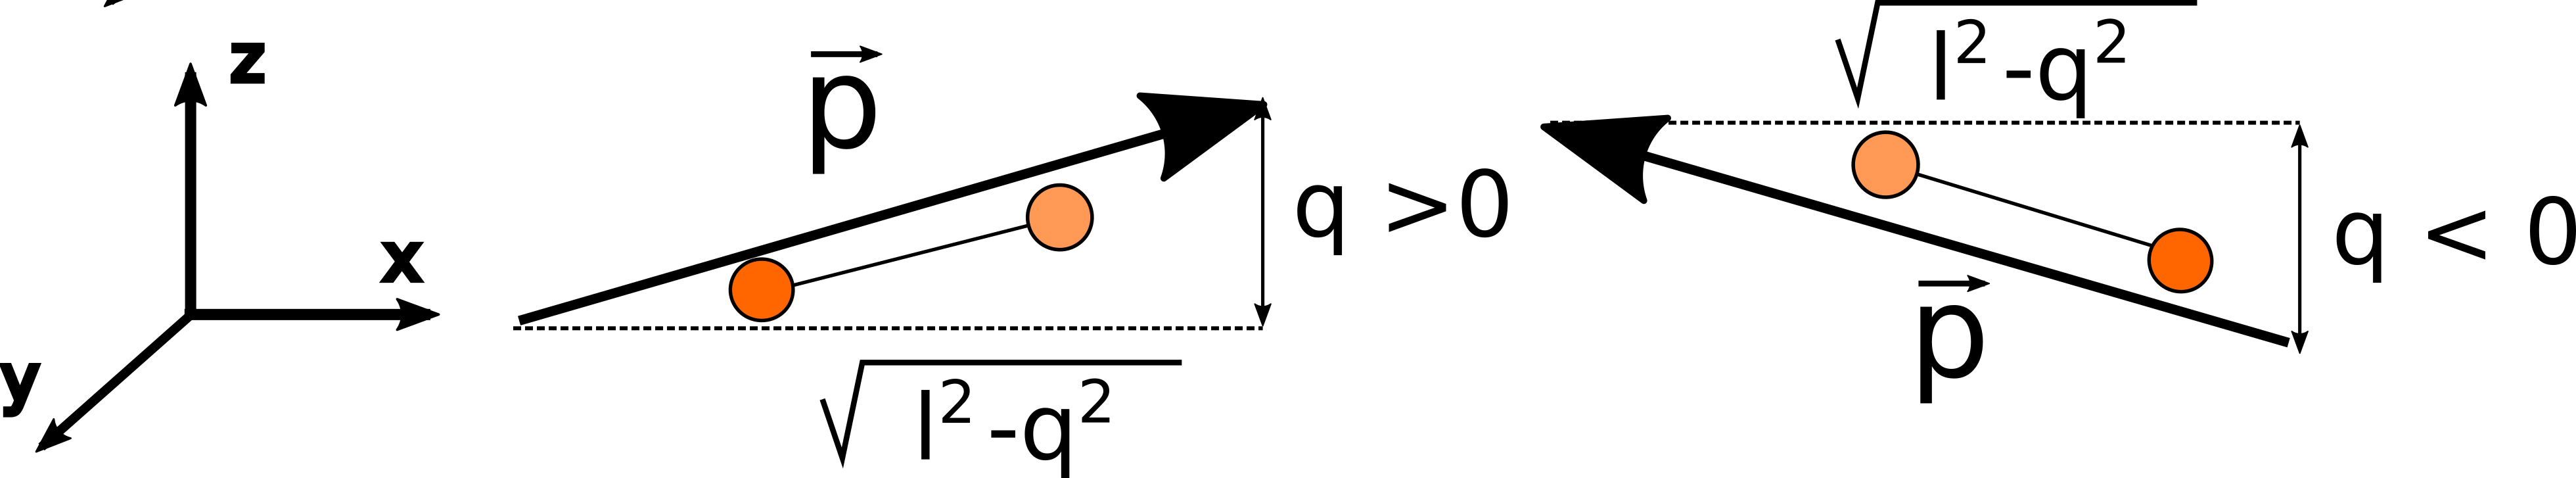
\includegraphics[width=0.8\linewidth]{graphics/DimerQParameterization.png}
		\caption{PLACEHOLDER}
		\label{Fig::DimerMapping}
	\end{figure}
	This is achieved by adding a factor $m = 2$ into the $J_\delta \cos \left(m \Delta \vartheta_{i, j}\right)$ terms. As stated in \autoref{Section::Silicon}, the dimers are buckled by  $18^{\circ}$ corresponding to a an angle $\vartheta^\pm=	\pm 72^\circ \approx	\pm \tfrac{2}{5} \pi $~. The equilibrium positions of \autoref{Eq::XY-Hamilton-Field} are determined by the symmetry breaking field and the parameter $p$ since the interaction is $O(2)$-symmetric. The minima satisfy
	\begin{equation}
		\cos \left(p \vartheta^\pm\right) =	-1~, \qquad \text{implying that} \qquad p \approx 2.57 ~,
	\end{equation}
	to ensure to reproduce the experimental equilibrium positions. The resulting potential of the symmetry breaking field is shown in \autoref{Fig::XY-Silicon-Potential}. \\
	\begin{figure}[htp]
		\centering
		\includegraphics[width=0.8\linewidth]{graphics/XY-Silicon-potential.png}
		\caption{The external field in combination with the restriction of $\vartheta$ leads to  the shown potential. The angle is measured from the $(110)$ axis for illustration purposes. The Dynamics of the dimers for sufficiently low temperatures will take place around $\vartheta =	0$, the bucklings of $\vartheta =	\pm \tfrac{1}{2} \pi$ will almost never be reached.}
		\label{Fig::XY-Silicon-Potential}
	\end{figure}
	A suitable order parameter for this model is
	\begin{equation} \label{Eq::Si-Order-Param}
		M_L =	\frac{1}{L^2} \sum_{i,j} m(\vartheta_{i, j}) \qquad \text{with} \qquad	m(\vartheta) =	\sin \left(\tfrac{p}{2} \vartheta\right) ~,
	\end{equation}
	as the $m(\vartheta)$ have maxima at $\vartheta^{+}$ and minima at $\vartheta^{-}$ satisfying $m(\vartheta^+) =	- m (\vartheta^-)$.
	
	Since in the XY-model the natural conjugated coordinate is the angle $\vartheta$ and therefore the equations of motions \autoref{Eq::Langevin-eq-motion-set-x} have to be adapted to rotary motion. The velocity is replaced by the angle velocity $\alpha$ in this case.
	
	\autoref{Eq::XY-Hamilton-Field} yields the force
	\begin{equation} \label{Eq::Potential-Derivative}
		\begin{split}
			\frac{\partial V(\{\vartheta\})}{\partial \vartheta_{i, j}} = ~~~& J_\parallel m \Big( \sin \left(\vartheta_{i,j} - \vartheta_{i + 1, j} \right) +   \sin \left(\vartheta_{i,j} - \vartheta_{i-1, j} \right) \Big)	 \\
			+ &J_\parallel m \Big( \sin \left(\vartheta_{i,j} - \vartheta_{i, j+1} \right) +  \sin \left(\vartheta_{i,j} - \vartheta_{i, j-1} \right) \Big) \\
			+ &h p \sin(p\vartheta_i)~.
		\end{split}
	\end{equation}
	Eventually, the langevin equations to integrate become
	\begin{align}
		&\frac{\text{d}}{\text{dt}} \vartheta_{i,j}(t) =	 \omega_{i,j}(t)~, \label{Eq::Si-Langevin-theta} \\
		&\frac{\text{d}}{\text{dt}} \omega_{i,j}(t) =	- \frac{\eta}{I} \omega_{i,j}(t) - \frac{1}{I}\frac{\partial V(\{\vartheta\})}{\partial \vartheta_{i,j}} + \sqrt{\frac{2 k_B T \eta}{I^2}} \Gamma(t)~, \label{Eq::Si-Langevin-omega}
	\end{align}
	with $\frac{\partial V(\{\vartheta\})}{\partial \vartheta_{i,j}}$ given in \autoref{Eq::Potential-Derivative}. The implementation of the solution of this coupled set of stochastic differential equations will be the subject of the next section.
	
	\begin{equation}
		\ddot{\vartheta}_{i, j} =	- \frac{\eta}{I} \dot{\vartheta}_{i, j} - \frac{1}{I} V_{i,j}' + \sqrt{\frac{2 k_B T \eta}{I^2}} \Gamma_{i,j}
	\end{equation}
	\chapter{Implementation and Results} \label{Chapter::Implementation-Results}
	To reduce finite size corrections it is beneficial to consider as large systems as possible. Combined with the critical slowing down described in  \autoref{Section::Dynamic-Scaling} the problem at hand inherently generates an arbitrarily large computational cost. On top comes the stochastic nature of the system, requiring to run many simulations to extract ensemble averages, as well as the need to avoid discretization errors and ensure convergence when implying \autoref{Eq::BBK-method} by choosing a small $dt$. This makes an efficient and fast implementation a crucial part of our investigations.
	\section{GPU programming}
	Besides the difficulties just described, there is an advantage that can be made use of. The langevin equations for the different lattice sites may be coupled through the potential \autoref{Eq::Potential-Derivative}, but the integration step for $t + dt$ only depends of the $\vartheta_{i, j}(t)$ of the previous step, meaning that the integrations can be performed simultaneously. This allows for heavy parallelization, making the problem predestined for a GPU implementation. \\
	
	The main difference between a conventional single core implementation on a central processing unit (CPU) and one on a graphical processing unit (GPU) is the number of processing cores involved. While CPUs only have few ($\sim 10$) powerful processing cores, GPUs are made up of more than $\sim 10^4$ cores. The CPU solves problems in a sequential matter, doing calculation after calculation making it suitable for usecases where the next step directly depends on the on before. In contrast, the GPU is able to perform many independent calculations real time simultaneously on its different cores. In situations where this is applicable, GPU implementations yield a significant speedup of up to a factor of $10^3$. A concept of the different solution approaches is shown in \autoref{Fig::CPU-vs-GPU}.\\
	\begin{figure}[htp]
		\centering
		
\includegraphics[width=0.8\linewidth]{graphics/CPU-vs-GPU.png}
		\caption{A CPU using single core processing would integrate the langevin equation for lattice site $i$ and move on to site $i+1$. The use of multi core processing would allow the CPU to integrate 4 sites simultaneously. In contrast, using GPU programming enables to evaluate the langevin equation at about $10^4 - 10^5$ sites at the same time.}
		\label{Fig::CPU-vs-GPU}
	\end{figure}
	
	For performance reasons the implementation took place (?) in \texttt{C++} using \texttt{Thrust} \cite{thrust} as high level interface for Nvidia's parallel computing platform \texttt{Cuda} \cite{cuda}. The source code can be found at \texttt{https://github.com/andiw99/Master-Arbeit}. The architecture is inspired by Ahnert et al.'s work \cite{ahnert2014solving}.
	\section{Benchmarks}
	Since an analytic solution of our model is intractable, proper benchmarks are vital to ensure the correctness of our simulation. Furthermore the stepsize used in \autoref{Eq::BBK-method} has to be analyzed to ensure convergence as well as a balance between the discretization error and efficiency.
	
	The Benchmarks that were conducted are
	\begin{itemize}
		\item the statistics of independent harmonic oscillators with thermal coupling,
		\item the equilibrium distribution of particles in a cosine potential,
		\item the equilibrium distribution of a system composed of two particles in a cosine potential with cosine interaction
	\end{itemize}
	The equation that describes the time evolution of probability densities of brownian motion is the \textbf{Fokker-Planck equation}. When talking about the probability density $p(x, v, t)$ in terms of particle velocity $v$ and position $x$ it is often referred to as the \textbf{Klein-Kramers-} or \textbf{Smoluchowski} equation and written as
	\begin{equation} \label{Eq::Klein-Kramers}
		\frac{\partial}{\partial t} p(x, v, t) = \left(-\frac{\partial}{\partial x} v + \frac{\partial}{\partial v} \left(\eta v - \frac{1}{m} \frac{\partial}{\partial x} V(x) \right) + \frac{\eta k_B T}{m} \frac{\partial}{\partial v^2}\right)p(x, v, t) ~.
	\end{equation}
	The Fokker-Planck equation and the langevin equations (\autoref{Eq::Langevin-eq-motion-set-x} and \autoref{Eq::Langevin-eq-motion-set-p}) are virtually identical and can be converted into each other. Ensemble averages over paths of langevin equations result in the probability distribution satisfying \autoref{Eq::Klein-Kramers}. The steady state distribution of the Fokker-Planck equation is the canonical distribution
	\begin{equation} \label{Eq::Canonical-Dist}
		p(x, v) \propto e^{\beta \left( \tfrac{1}{2} m v^2 + V(x)\right)},
	\end{equation}
	allowing for an easy way to verify long term behavior.
	\subsection{Thermal harmonic oscillators}
	For a quadratic potential
	\begin{equation}
		V(x) =	\tfrac{1}{2} \omega^2 x^2,
	\end{equation}
	the Fokker-Planck equation is analytically solvable \cite{risken1996fokker}. This makes it ideal to confirm correct dynamics of the simulation. The analytic solution for the second moment of $x(t)$ reads
	\begin{equation}
		\left \langle x^2 \right \rangle (t)  =	\frac{\eta {k_B T}}{m (\lambda_+ - \lambda_-)^2} \left[ \frac{\lambda_+ + \lambda_-}{\lambda_+ \lambda_-} + \frac{4}{\lambda_+ + \lambda_-} \left(e^{- (\lambda_+ + \lambda_-) t} - 1\right) - \frac{1}{\lambda_+} e^{-2\lambda_+ t} - \frac{1}{\lambda_-} e^{- 2 \lambda_- t}\right],
	\end{equation}
	with
	\begin{equation}
		\lambda_{\pm} =	\frac{1}{2} \left(\eta \pm \sqrt{\eta^2 - 4 \omega^2}\right)
	\end{equation}
	In \autoref{Fig::MSD-Comparison} we compare $\left \langle x^2 \right \rangle (t)$ calculated from $\approx65000 $ path, simulated by either the Euler-Maruyama- or the BBK method, with the theoretical result. The BBK algorithm with $dt =	0.05$ and the Euler-Maruyama method with $dt =	0.001$ yield similar small deviations from the theoretical curve, suggesting that the BBK method can be used up to much larger stepsizes. Besides, the validity of both methods for thermal harmonic oscillators is given for both methods for small enough stepsizes.
	
	\begin{figure}[htp]
		\begin{subfigure}{0.5\textwidth}
			\centering
			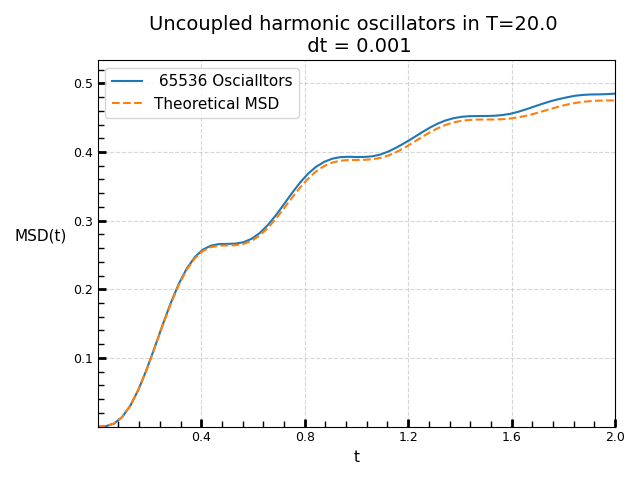
\includegraphics[width=0.8\linewidth]{graphics/MSD-Euler-0.001.png}
			\caption{The Euler-Maruyama method with a stepsize of $dt=0.001$ results in small but noticeable deviations.}
		\end{subfigure}
		\begin{subfigure}{0.5\textwidth}
			\centering
			\includegraphics[width=0.8\linewidth]{graphics/MSD-BBK-0.005.png}
			\caption{The BBK method with a stepsize of $dt=0.005$ reproduces the theoretical curve very well.}
		\end{subfigure}  \\
		\begin{subfigure}{0.5\textwidth}
			\centering
			\includegraphics[width=0.8\linewidth]{graphics/MSD-Euler-0.05.png}
			\caption{The Euler-Maruyama method with a stepsize of $dt=0.05$ results in large deviations.}
		\end{subfigure}
		\begin{subfigure}{0.5\textwidth}
			\centering
			\includegraphics[width=0.8\linewidth]{graphics/MSD-BBK-0.05.png}
			\caption{The BBK method with a stepsize of $dt=0.05$ results in small but noticeable deviations.}
		\end{subfigure}
		\caption{The calculated $\left \langle x^2 \right \rangle (t)$ of thermal harmonic oscillators are compared for the Euler-Maruyama- and the BBK method with different stepsizes}
		\label{Fig::MSD-Comparison}
	\end{figure}
	
	\subsection{Particles in a cosine potential}
	Another valuable Benchmark is the edge case of weakly interacting particles with $J=0$. We will confirm that probability distribution calculated from  $???$ particle paths will approach the theoretical equilibrium distribution given by inserting \autoref{Eq::XY-Hamilton-Field} for $J_\delta =	0$ into \autoref{Eq::Canonical-Dist}. \\
	
	In \autoref{Fig::Cos-Prob-Dist} we show the calculated integrated probability density $p(x) =	\int_{}^{} p(x, v) dv$ is plotted. The BBK method shows virtually no discretization errors up to a stepsize of $dt =	0.05$. For the Euler-Maruyama method large discretization errors show up for stepsizes one magnitude smaller. \\
	
	Again, for sufficiently small stepsizes the long term behavior of our simulation is  verified.
	
	\begin{figure}[htp]
		\begin{subfigure}{0.5\textwidth}
			\centering
			\includegraphics[width=0.8\linewidth]{graphics/Distribution-Euler-0.005.png}
			\caption{The Euler-Maruyama method shows significant discretization errors regarding $p(x)$ even for a comparatively small stepsize of $dt =	0.005$.}
		\end{subfigure}
		\begin{subfigure}{0.5\textwidth}
			\centering
			\includegraphics[width=0.8\linewidth]{graphics/Distribution-BBK-0.05.png}
			\caption{The BBK method shows almost no deviation from the theoretical $p(x)$ even for a stepsize of $dt =	0.05$.}
		\end{subfigure}
		\caption{The integrated probability distributions $p(x)$ calculated from ??? particle paths are compared to the theoretical equilibrium distribution for the Euler-Maruyama method and the BBK Algorithm. It was made sure that the systems were completely relaxed, meaning that the effects of the starting position vanished and the shape of the probability distribution did not change anymore.}
		\label{Fig::Cos-Prob-Dist}
	\end{figure}
	
	\subsection{Two interacting particles in a cosine potential}
	The third benchmark has the purpose of verifying the correct behavior of the interaction. Since the equilibrium distribution becomes a high dimensional function $p(\{x_i\}, \{v_i\})$, a suitable representation is possible in the case of system consisting of two particles. The object of examination is again the equilibrium probability distribution of the Fokker-Planck equation.\\
	
	In \autoref{Fig::Pair-Prob-Dist} we now show cuts of the integrated probability density $p(x_1, x_2) =	\int_{} p(x_1, x_2, v_1, v_2) dv_2 dv_1$ with a constant $x_2$. It is verified that simple interacting systems are driven to their equilibrium by the method of langevin integrations. The statistical- and discretization errors vanish for many samples and small stepsizes.
	
	\begin{figure}[htp]
		\begin{subfigure}{0.5\textwidth}
			\centering
			\includegraphics[width=0.8\linewidth]{graphics/Pair-Equil-Dist-20.png}
			\caption{Different x2s?}
		\end{subfigure}
		\begin{subfigure}{0.5\textwidth}
			\centering
			\includegraphics[width=0.8\linewidth]{graphics/Pair-Equil-Dist-20.png}
			\caption{Different Temperatures?}
		\end{subfigure}
		\caption{Cuts of the integrated probability distributions $p(x_1, x_2)$ with a constant $x_2$ calculated from ??? particle paths are compared to the theoretical equilibrium distribution. It was made sure that the systems were completely relaxed, meaning that the effects of the starting position vanished and the shape of the probability distribution did not change anymore.}
		\label{Fig::Pair-Prob-Dist}
	\end{figure}
	
	\section{Results}
	In the following the results of the explained simulation will be presented. We will start with the examination of the critical exponents of our model. \\
	
	The parameters will be measured in units of $J_\perp =	1$ and the initially used ratio $J_\parallel /	J_\perp =	31.1$ is the one from Brand et. al \cite{brand2023dimer}. The external field $h =	5$ is chosen small compared to $J_\parallel$ to ensure approximate validity of \autoref{Eq::Crit-Temp-XY}. The strength of $h$ should not influence the kind of phase transition we observe as long as it is finite, but may influence $T_c$. Both coupling strengths are negative to reproduce the c(4x2) symmetry. To conclude, as long as not otherwise stated, the in the following used model parameters of \autoref{Eq::XY-Hamilton-Field} are
	\begin{equation}
		J_\perp =	-1~, \qquad \qquad J_\parallel =	-31.1 \qquad \text{and} \qquad h =	5.
	\end{equation}
	The dampening is set to $\eta =	1.5$. Our method of correlation length extraction \autoref{Section::Corr-Lenght-Calculation} works best if $\xi_\delta \ll L_\delta$. Since the Si(001) surface exhibits a large correlation length anisotropy $\tfrac{(\xi_\parallel /	a_\parallel)}{(\xi_\delta /	a_\delta)} \approx 10 $, it is useful to ensure that the system sizes share a similar ratio. This way we can analyze larger correlation lengths without increasing the computational cost. The following systems have a ratio of $\tfrac{L_\parallel}{L_\perp} =	8$ if not stated otherwise. The used stepsize is $dt = 0.01$
	\subsection{static scaling}
	Since the phase transition of the Si(001) surface seems to belong to the Ising universality class \cite{brand2023critical}, our simulation should reproduce this. The XY model with a $p$-fold symmetry breaking external field belongs to the Ising universality class for $p=2$ \cite{jose1977renormalization}, but the question remains if this is still true for our adaptation (\autoref{Sec::XY-to-Silicon}) with a rational number $p \approx 2.57$. \\
	
	Therefore, the finite size techniques and the Binder cumulant described in \autoref{Section::FSS} and \autoref{Sec::Binder-Cumulant} are employed to extract the critical exponent. The magnetization is calculated using \autoref{Eq::Si-Order-Param}. We initialize totally ordered systems as suggested in \cite{binder2022monte}, that is all dimers are alternatively buckled. We run multiple small independent systems simultaneously on a single GPU to achieve optimal parallelization. We run long simulations to ensure the thermalization of the systems. During the run, we document the Binder cumulant $U_L(t)$ to be able to afterwards determine a timepoint $t_{equil}$ after which we judge the cumulant to be equilibrated. The cumulant is subject to statistical fluctuations, so to obtain useful averages it can be made use of the ergodic hypotheses. Instead of running many simulations and averaging the latest value of $U_L$, we simulate systems for long times $t_{long}$ and calculate the ensemble average as the time average
	\begin{equation} \label{Eq::Mean-Ergodic-Hypo}
		\overline{U}_L =	\frac{1}{(t_{long} - t_{equil})} \int_{t_{equil}}^{t_{long}} U_L(t) dt~.
	\end{equation}
	In \autoref{Fig::Binder-Cum-Result} the results for ??? systems simulated until $t_{long} = ???$ are shown for temperatures very close to $T_c$. The critical point was approached by estimating the critical temperature with \autoref{Eq::Crit-Temp-XY} yielding $T_c^{est} \approx 0.618$, examining the general area for the phase transition and then iteratively closing in. The more precise $T_c$ shall be determined, the closer the temperatures have to lie at $T_c$. The closer two temperatures lie, the easier it is for statistical fluctuations to smear their relative position and therefore the more averages you need. The same is true for the calculation of the critical exponent $\nu$. The derivative $\tfrac{\partial U_L}{\partial \varepsilon}$ is calculated through a simple central difference. Afterwards the function \autoref{Eq::FSS-dU_dT} is fitted to $\tfrac{\partial U_L}{\partial \varepsilon} (L)$. The result $\nu =	1.04$ is in good agreement with the theoretical critical exponent of the Ising model $\nu =	1$.
	\begin{figure}[htp]
		\begin{subfigure}{0.5\textwidth}
			\centering
			\includegraphics[width=0.8\linewidth]{graphics/cum_time_avg.png}
			\caption{The Binder cumulants intersect at $T_c =	0.953$. The intersection is determined by the minimum squared error between the cumulants.}
		\end{subfigure}
		\begin{subfigure}{0.5\textwidth}
			\centering
			\includegraphics[width=0.8\linewidth]{graphics/critical_exponent_time_avg.png}
			\caption{The derivatives $\frac{\partial U_L}{\partial \varepsilon}$ scale like $\propto L^\nu$. The fitting results in $\nu = 1.04$ which is in good accordance with the Ising model.}
		\end{subfigure}
		\caption{The results for $\overline{U}_L$ of ??? averaged systems of different sizes simulated for a time of $t_{long} =	??? $ are shown. The estimated equilibration time is $t_{equil} =	??? $.}
		\label{Fig::Binder-Cum-Result}
	\end{figure}
	The matching of the static critical exponent verifies our numerics as well as the assumption that our modification of the XY model still belongs to its expected universality class. \\
	\begin{figure}[htp]
		\centering
		\includegraphics[width=0.8\linewidth]{graphics/Tc-L.png}
		\caption{The dependence of the critical temperature $T_c$ is calculated in dependence of the system size $L$. The x-axis shows the smaller system size $L_{min}$. The binder cumulant intersection is always calculated with twice the small system size $L_{max} =	2 L_{min}$.}
		\label{Fig::Tc-L-dependence}
	\end{figure}
	In \autoref{Fig::Tc-L-dependence} the relation of the binder cumulant intersection aka our estimate for $T_c$ is shown in dependence of the system size. The datapoints show the intersection of two curves $U_{L_1}(T)$ and $U_{L_2}(T)$ with $L_2 =	2 L_1$. The errorbars are assumed to be $\Delta T_c = \tfrac{1}{2} dT$ with $dT$ being the stepsize between the recorded temperatures. This error is probably an overestimation. The difference in $T_c(L_1, L_2)$ is negligable between $T_c(48, 96)$ and $T_c(64, 128)$ so we conclude that finite size effects on the critical temperature determination vanish on these length scales. For $L_1 =	64$ the measurement was continued to minimize the stepsize to $dT /	2$. A smaller $dT$ leads to a systematically slightly larger $T_c$ as the intersection is usually located at the convex part of $U_L(T)$.  \\
	\subsection{dynamic scaling}
	The dynamic universality classes are subgroups of the static universality classes and our model could very well be in a different dynamic universality class than the 2D Ising model. In the following multiple methods will be employed to extract the dynamic critical exponent $z$.
	
	\subsubsection{The Kibble-Zurek mechanism}
	The first method will be the extraction through \autoref{Eq::KZM-scaling} and the Kibble-Zurek mechanism. Since we already gained knowledge of $\nu$ we can fit the exponent $\nu /	(1 + \nu z)$ to quenched correlation lengths deduce $z$. \\
	
	The used quench protocol, i.e the manner in which the system is cooled down, will be a simple isotropic, linear quench like \autoref{Eq::Linear-Quench}. The starting temperature $\varepsilon(t_{start})$ is chosen to be sufficiently far away to observe adiabatic system evolution before crossing the freezeout point $\varepsilon(t_{start}) < \varepsilon(\hat{t})$. The end temperature $\varepsilon(t_{end})$ is chosen in symmetric distance from the transition point $|\varepsilon(t_{start})|=|\varepsilon(t_{end})|$. \\
	
	In \autoref{Fig::Quench-Result} the results for the quench of our system are shown. A fit of the frozen correlation lengths $\hat{\xi}$ to \autoref{Eq::KZM-scaling} is performed in \autoref{Fig::Quench-Result-c} and \autoref{Fig::Quench-Result-d}. Only the datapoints in the phase space where the Kibble-Zurek mechanism should be valid are used. It was made sure that $\hat{\xi}_\delta \ll L_\delta$ so that \autoref{Section::Corr-Lenght-Calculation} is still applicable. The extracted KZM exponent of $\nu /( 1 + \nu z)$ is unusually large and suggests that $z < 2$. \\
	
	A KZM independent z extraction method is needed to verify the correct critical exponent.
	\begin{figure}[htp]
		\begin{subfigure}{0.5\textwidth}
			\centering
			\includegraphics[width=0.8\linewidth]{graphics/xix-process.png}
			\caption{The time-resolved quench-process $\xi_x(t)$ for different quench timescales is shown for the system sizes $L_x =	600, 1200$.}
		\end{subfigure}
		\begin{subfigure}{0.5\textwidth}
			\centering
			\includegraphics[width=0.8\linewidth]{graphics/xiy-process.png}
			\caption{The time-resolved quench-process $\xi_x(t)$ for different quench timescales is shown for the system sizes $L_y =	75, 150$.}
		\end{subfigure} \\
		\begin{subfigure}{0.5\textwidth}
			\centering
			\includegraphics[width=0.8\linewidth]{graphics/xix-quench-scaling.png}
			\caption{The frozen correlation length $\hat{\xi}_x(\tau)$ depending on the quench timescale is investigated. A fit of the data to \autoref{Eq::KZM-scaling} is calculated and drawn in the appropriate area.}
			\label{Fig::Quench-Resulb-c}
		\end{subfigure}
		\begin{subfigure}{0.5\textwidth}
			\centering
			\includegraphics[width=0.8\linewidth]{graphics/xiy-quench-scaling.png}
			\caption{The frozen correlation length $\hat{\xi}_y(\tau)$ depending on the quench timescale is investigated. A fit of the data to \autoref{Eq::KZM-scaling} is calculated and drawn in the appropriate area.}
			\label{Fig::Quench-Resulb-d}
		\end{subfigure}
		\caption{The results of the quenches are investigated using the Kibble Zurek mechanism. The Kibble-Zurek mechanism is valid where the system is at the start of the quench able to adiabatically follow the process. When the quench is so fast that the system cannot follow the quench even at the start, the frozen correlation length is the equilibrium correlation length of the starting temperature and no scaling is observed.}
		\label{Fig::Quench-Result}
	\end{figure}
	\subsubsection{Relaxation of the Binder cumulant}
	A simple way to examine the dynamic critical exponent is to consider the relaxation of the Binder cumulant including finite size scaling. This method was introduced by Li et. al \cite{li1995dynamic} and will be used in the following to extract the dynamic critical exponent. \\
	
	The basis is the time-resolved finite size scaling of the $(n)-$th moment of the magnetization
	\begin{equation} \label{Eq::Dynamic-FSS-M}
		M^{(n)}(t, \varepsilon, L) = b^{-n \beta / \nu} M^{(n)}(b^{-z}t, b^{1 /	\nu} \tau, b^{-1} L) ~,
	\end{equation}
	with $b =	\tfrac{L}{L'}$ being the spatial rescaling factor. Janssen et. al \cite{janssen1989new} determined that the initial correlation length must be very short for \autoref{Eq::Dynamic-FSS-M} to be valid. Therefore the investigated systems will be prepared in a high temperature, low order state.
	Following the definition of the Binder cumulant  \autoref{Eq::Def-Binder-Cum}, one can relate the Binder cumulant of systems of different sizes at the critical point $\varepsilon =	0$ by
	\begin{equation}
		U(t, 0, L_1) =	U(b^{-z} t, 0, L_2)~, \qquad \text{with} \qquad b = \frac{L_1}{L_2}
	\end{equation}
	The exponent $z$ is easily obtained by searching a time rescaling factor $b^{-z}$ such that the recorded curves for $U_{L_1}$ and $U_{L_2}$ collapse. Since the sample systems are prepared in a high temperature state where $U_L =	3$, we expect a relaxation from this value to the equilibrium $U_L^*$ which is, at $\varepsilon =	0$, the same for every system size.
	\begin{figure}[htp]
		\centering
		\includegraphics[width=0.8\linewidth]{graphics/cum-over-time-scan.png}
		\caption{The best rescaling of $U_{L_1} \rightarrow U_{L_2}$ is selected by minimizing the squared error between the interpolated curves. The result of the rescaling from $64 \rightarrow 128$ yields a dynamic critical exponent of $z = 2.08$, close to the best known value for the Ising universality class (see \autoref{Table::Ising-crit-expo}). }
		\label{Fig::Cum-Relax-z-extrac}
	\end{figure}
	The results for the rescalings $32 \rightarrow 64$ and $64 \rightarrow 128$ calculated from ??? sample paths are shown in \autoref{Fig::Cum-Relax-z-extrac}. The rescaling $64 \rightarrow 128$ is to be trusted more than the $32 \rightarrow 64$ since it minimizes the finite size corrections to the scaling law \autoref{Eq::Dynamic-FSS-M}. Its result $z =	2.08$ is very close to the best available dynamical critical exponent of the Ising model $z_{Ising}=2.14$.With this the calculated KZM exponent of $\nu /	(1 + z\nu) = 0.33	$ stands in harsh contradiction to the exponent obtained directly from the quench $\nu /	(1 + z\nu) = 0.45$. Since it is from symmetry considerations very plausible that our model for silicon would show the Ising dynamical exponent, we would expect that the deviation stems from the Kibble-Zurek scaling. Since the system sizes used in the quenches is already very large, strong finite size corrections to the Kibble-Zurek scaling can be ruled out as cause of the deviation. The same is true for the discretization error of our stepsize since the same quenches have been recalculated with a smaller stepsize. Since the correctness of our simulation has otherwise been verified, the most sensible explanation for the large Kibble-Zurek scaling exponent is that the cause has to be a systematic difference in the expected Kibble-Zurek mechanics (???). An idea could be the existence of subleading scalings like reported in \cite{ladewig2020kibble} caused by other scaling fields than the temperature. In our case such a scaling field could be the strength of the external potential $h$. \\
	
	In the following we will investigate the effect of the strength of $h$ on the dynamical critical exponent as well as the Kibble-Zurek exponent.
	\subsection{The correlation length amplitudes $\xi_\delta^+$}
	The static scaling law of the correlation length $\xi_\delta$ above the critical temperature ($\varepsilon > 0$) given by \autoref{Eq::RG-xi-scaling} can be rewritten as
	\begin{equation} \label{Eq::Xi-divergence-amplitude}
		\xi_\delta (\varepsilon) = \xi_\delta^{+} \varepsilon^{-\nu}~,
	\end{equation}
	with the so called correlation length amplitude $\xi_\delta^{+}$. The $+$ sign denotes the amplitude above the critical temperature. The correlation lengths in the Ising model are directly related to the temperature and the coupling constants $J_\delta$. Their relation above the critical temperature is given by \autoref{Eq::Ising-Corrlength-Coupling}. An expansion of \autoref{Eq::Ising-Corrlength-Coupling} around the critical temperature $T_c$ leads to a simple relation between the coupling constants and the correlation length amplitudes,
	\begin{equation} \label{Eq::Ising-Ampl-ratio-xi}
		\sinh \left(\frac{2 |J_\delta|}{k_B T_c}\right) =	\frac{\xi_\delta^+ / a_\delta}{\xi_{\overline{\delta}}^+ / a_{\overline{\delta}}}~.
	\end{equation}
	This relation is exceptionally useful, as it can be used to determine the coupling energies $J_\delta$ from the measured correlation lengths and critical temperatures as is done in \cite{brand2023dimer}, \cite{brand2023critical}. The value that is obtained here for the amplitude ratio in units of the lattice constants is $({\xi_\parallel^+ / a_\parallel}) \big/	({\xi_{\perp}^+ / a_{\perp}}) =	10.3$.  \\
	
	A relation like \autoref{Eq::Ising-Ampl-ratio-xi} for the XY model with a symmetry breaking field is not known at the moment and efforts to derive one were unsuccessful. So a direct relation of the correlation length ratio to the model couplings $J_\delta, h$ and even $p$ is not possible. But since the symmetry broken XY model and the Ising model have shown to behave quite similar in the previous investigations, it is reasonable to examine the correlation length amplitude ratio for the Ising coupling constant ratio $J_\parallel /	J_\perp =	31.1$. \\
	
	The amplitude ratio is investigated by preparing the system in a random state and letting it relax at a fixed temperature $T \gtrsim T_c$. To judge whether the system is relaxed and at the same time obtain a precise value for the equilibrium correlation length, $\xi$ is monitored on the run in the spirit of \autoref{Eq::Mean-Ergodic-Hypo}. Every $n_s =100$ steps, $\xi_\delta$ is calculated and saved. After reaching a minimum step threshold, every $n_\sigma =	5 n_s$ steps also the mean $\overline{\xi}_\delta$ as well as its error $\sigma_{\overline{\xi}_\delta}$ is calculated. The correlation of $\xi(t)$ and $\xi(t + n_s dt)$ has to be taken into consideration if $n_s dt< \tau$ (see \autoref{Section::Error-Calc}). When calculating mean and error, a fraction $p_\tau =	1 /	2$ of correlation lengths is ignored in order to account for the equilibration of the system. After falling below a maximum relative error of $\sigma_{max} /	\overline{\xi}_\delta =	0.01$ for both directions, the run is terminated. The used system size is chosen as large as numerically feasible to minimize finite size effects around the critical temperature $T_c$. \\
	\begin{figure}[htp]
		\begin{subfigure}{0.5\textwidth}
			\centering
			\includegraphics[width=0.95\linewidth]{graphics/amplitude-inverse-xi.png}
		\end{subfigure}
		\begin{subfigure}{0.5\textwidth}
			\centering
			\includegraphics[width=0.95\linewidth]{graphics/amplitude-xi-divergence.png}
		\end{subfigure}
		\caption{\textbf{(a)} The inverse correlation length $\xi^{-1}$ of a system of size $L_x =	?$ equilibrium is measured and shown for temperatures $T \gtrsim T_c$. The line is a linear fit with the parameters $\xi_\delta^+$ and $T_c$. \textbf{(b)} The divergence of $\xi$ is measured around $T \gtrsim T_c$. The line is calculated by \autoref{Eq::Xi-divergence-amplitude}, using the parameters obtained by the fit of (a).}
		\label{Fig::Amplitude-Result}
	\end{figure}
	The results for the equilibrium $\xi_\delta$ for a system of size $L_x = ? $are shown in \autoref{Fig::Amplitude-Result}. To extract the correlation length amplitude $\xi^+_\delta$, the scaling of $\xi_\delta^{-1}$ was considered, which is given by
	\begin{equation}
		\xi_\delta^{-1}(T) =	\frac{1}{\xi_\delta^+} \left(\frac{T - T_c}{T_c}\right) =	- \frac{1}{\xi_\delta^+} + (T_c \xi_\delta^+)^{-1} T ~,
	\end{equation}
	if the result $\nu =	1$ is used. Therefore $\xi$ behaves linearly in $T$ around the critical point. Which datapoints shall be included is decided by selecting the best linear regression in the parameters of $\xi_\delta^+$ and $T_c$ of at least 4 consecutive datapoints that agree with the previously determined critical temperature $T_c^{U_L}$. The quality of the fit is determined by the $r^2$-value of the regression. A minimum $r^2$-value of $r_{min}^2 = 0.98$ is required to accept a successful fit. (TODO) maybe just choose the regression that has a minimum r² value and is as close to Tc as possible?) Close to $T_c$ finite size effects become visible. To illustrate this, $\xi$ is recalculated at the questionable datapoints for a system of size $L_x' =	2 L_x$. At this point I am not sure why the correlation length becomes smaller already a temperatures slightly larger than $T_c$, the RG theory actually predicts that the maximum of $\xi$ should be shifted to a lower temperature?. The correlation length ratio of $\xi_\parallel^+ / \xi_\perp^- = ? $ is smaller than expected for the Ising model. Reasons for this could be influences of the symmetry breaking field and structural difference in the relationship of the coupling constants and the correlation lengths. The influence of the symmetry breaking field on the amplitude ration will be investigated in the following.
	\subsection{quantitative}
	Since the dimer interaction is a kind of dipole interaction \cite{pillay2004revisit}, our XY-model interaction might not reproduce quantitative results of the real system. In the following some quantitative considerations will be done anyway. \\
	
	Since the numbers used in a simulation are all dimensionless, one has to think about what those numbers represent in physical quantities. Since the mass $m$, or for rotational motion equivalently the moment of inertia $I$, is not implemented into the simulation, it is easiest to measure all quantities in multiples of $I$. Natural units will be used in the following. The moment of inertia is approximated as two point masses $m_{Si} \approx 28u =	26 \text{ GeV}$ with a distance of $2r \approx 2 ~\text{\AA} \approx 10~ \text{keV}^{-1}$, yielding
	\begin{equation}
		I \approx 2m_{Si} r^2 \approx	2 \left(26 ~\text{GeV}\right) \left(5 ~\text{keV}^{-1}\right)^2 =	1300 \text{ meV}^{-1}~.
	\end{equation}
	The dimensionless angular velocity $\Omega$ in units of $I$ is
	\begin{equation}
		\Omega(t) =	I\omega(t)~.
	\end{equation}
	The dimensionless version of \autoref{Eq::Si-Langevin-omega} becomes
	\begin{equation} \label{Eq::Dimensionless-Omega}
		\begin{split}
			\Omega_{i,j}(t + dt) &=	\Omega(t) - \eta \Omega_{i,j}(t) \frac{dt}{I} - {I}\frac{\partial V(\{\vartheta\})}{\partial \vartheta_{i,j}} \frac{dt}{I} + \sqrt{\frac{2 T \eta}{I^2}} n(t) I \sqrt{dt} \\
			&=	\Omega(t) - \eta \Omega_{i,j}(t) d\sigma - \frac{\partial v(\{\vartheta\})}{\partial \vartheta_{i,j}} d\sigma + \sqrt{{2 \kappa \eta}} n(t) \sqrt{d\sigma}~,
		\end{split}
	\end{equation}
	with the dimensionless quantities
	\begin{align}
		&\sigma =	t /	I, \\
		&v(\vartheta) =	I V(\vartheta), \qquad \text{and} \\
		&\kappa =	IT.
	\end{align}
	The second line of \autoref{Eq::Dimensionless-Omega} is what is implemented in the simulation. To get the physical values, the equation has to be divided by the moment of inertia $I$. The position coordinate $\vartheta$ of the dimer however does not have to be converted since the dimensionless form of \autoref{Eq::Si-Langevin-theta}
	\begin{equation}
		\begin{split}
			\vartheta(t + dt) &=	\vartheta(t) + \Omega(t) d\sigma =	\vartheta(t) + I \omega(t) \frac{dt}{I} \\
			&= \vartheta(t) + \omega(t) dt
		\end{split}
	\end{equation}
	equals the dimensionful form. \\
	
	The used dimensionless stepsize of $d\sigma = 0.01$ corresponds to a physical stepsize of
	\begin{equation}
		dt = I d \sigma =	1300 \text{ meV}^{-1} \cdot 0.01 \approx 0.01 \text{ ns}~,
	\end{equation}
	which is very reasonable since this stepsize is of the order of magnitude of the fast hight temperature flipping of the dimers (source? BrandCritical). The dimensionless critical temperature has a value of
	\begin{equation}
		\kappa_c =	1300 \text{ meV}^{-1} \cdot 16.43 \text{ meV} \approx 22100~,
	\end{equation}
	using the experimental critical temperature $T_c =	16.43 \text{ meV}$ of Brand et. al \cite{brand2023dimer}.
	Assuming a ratio of $J_\parallel /	J_\perp =	31$, \autoref{Eq::Crit-Temp-XY} can be used to together with $T_c$ to estimate the values of $J_\delta$. We get
	\begin{equation}
		J_\perp =	2.66 \text{ meV} \qquad \text{and} \qquad J_\parallel = 82.46 \text{ meV}~,
	\end{equation}
	corresponding to the dimensionless values $j_\delta =	I J_\delta$ of
	\begin{equation}
		j_\perp =	3580 \qquad \text{and} \qquad j_\parallel =	110980~.
	\end{equation}
	The question now is how to choose $h$ in order not to change the phase transition again. Therefore a perturbation based version of \autoref{Eq::Crit-Temp-XY} including h would be very useful. And the dampening is also crucial to the timescales on which the system evolves. There is probably no way of estimating this? Or there might be one but that is surely not possible in 2 months...
	
	For the addition of h: you know the form of the phase diagram of the XY model, and I think you even know the kind of function it describes. What you probably don't know are the prefactors, etc. You can fit them but they probably are dependent on J? It is not dependent on $\eta$ at least. \\
	
	The equilibrium position of the dimers is determined by the strength of repulsion $J_\parallel$ and $J_\perp$, the amplitude of the symmetry breaking field $h$ and the position of its minima determined by the parameter $p$. In the case of ferromagnetic interaction, the equilibrium position is solely determined by $p = \tfrac{18}{7} $ which yields the experimental equilibrium position of $\vartheta^* =	\tfrac{7}{18} \pi = 70^\circ$ (measuring from the z-Axis). We can also infer that $p > 2$ as $p=2$ means that the equilibrium position of the symmetry breaking field is at $\vartheta = \pi /	2$, corresponding to a horizontal dimer. Since we see from DFT calculations that even the buckling itself without any constraint on the configuration decreases the energy, this is not realistic. The two constrains conclude to $p \in \left[2, 2.57\right]$ Consider now a specific lattice site of a system in total equilibrium, meaning that the site's buckling angle is $\vartheta =	\vartheta^*$ and the buckling angle of all its neighbors is $\vartheta_{NN} =	- \vartheta^*$. The condition that $\tfrac{\partial H(\vartheta)}{\partial \vartheta} \Big |_{\vartheta =	\vartheta^*} =	0$ gives
	\begin{equation} \label{Eq::Equilibrium-Position}
		-4 \sin(4 \vartheta^*) \left(\frac{J_\parallel + J_\perp}{h}\right) =	p \sin \left(\vartheta^* p\right)~.
	\end{equation}
	This is a transcendental That determines the parameter $p$ in dependence of the coupling constants, $h$ and the desired equilibrium position.
	For the experimental $\vartheta^*$, $\sin(4 \vartheta^*) \approx -1$, leading to the simpler form
	\begin{equation}
		4 \frac{J_\parallel + J_\perp}{h} =	p \sin(\tfrac{7\pi}{18} p)~.
	\end{equation}
	The right hand side of this equation is monotonically decreasing on the interval $\left[2, 2.57\right]$, so a solution is only possible if
	\begin{equation}
		\frac{J_\parallel + J_\perp}{h} \leq \frac{1}{4} \cdot 2 \cdot \sin (\frac{14}{18} \pi)  \approx \frac{1}{3}
	\end{equation}
	\subsubsection{Fitting the model parameters to DFT calculations}
	Numerous investigations calculated configuration energies of the Si(001) \cite{fu2001molecular, ramstad1995theoretical} surface by density functional theory (DFT) methods and fitted the Ising model parameters accordingly \cite{pillay2004revisit, inoue1994order, ihm1983structural, xiao2019spontaneous}. We can trace their path and use their configuration energies to get a feeling of the dimension of our coupling parameters.  \\
	
	The model in use has 4 parameters that influence the configuration energy, being the interaction couplings $J_\parallel, J_\perp$, the strength $h$ and the position, characterized by $p$, of the symmetry breaking field. Another unknown is the binding energy of the lowest configuration $E_0$, in our case being the absolute energy of the $c(4\times2)$ configuration. Since $p$ is inside a $cos(p\theta)$, the fitting of the model parameters will result in a 5-dimensional non linear system of equations, which could be a bit tedious to solve. An approximation that is probably still fairly accurate would be to determine p solely from the equilibration angle of the asymmetric $p(2\times1)_a$ configuration. Since in this configuration all dimers have the same buckling angle by definition, the dimer interaction cannot influence the equilibrium angle, since there is i.e. no repulsion involved that could shift the minimum of the symmetry breaking field. The caveat is that we have to assume that the surface configuration does not or only slightly change the strength and shape of the symmetry breaking field, which is in the real world system generated by the silicon bulk. If that's the case, the angle that is observed in the $p(2\times1)_a$ configuration directly determines $p$ since
	\begin{equation}
		\cos \left(\vartheta_{p(2\times1)_a} p \right) \approx -1 \qquad \Rightarrow \qquad  p =	\pi /	\vartheta_{p(2\times1)_a} ~.
	\end{equation}
	Pillay et. al \cite{pillay2004revisit} found an buckling angle of $\approx 17.2^\circ$ resulting in $\vartheta_{p(2 \times 1)_a} =	72.8^\circ$ and $p =	2.473$. With this simplification we obtain a linear system of equations
	\begin{align}
		&c(4\times2): 	\qquad \cos(4\vartheta^{(1)})&J_\parallel&+ \cos(4\vartheta^{(1)})&J_\perp&+\cos \left(\vartheta^{(1)}p\right) h =	E_0 \\
		&p(2\times2): 	\qquad \cos(4\vartheta^{(2)})&J_\parallel&+&J_\perp&+ \cos \left(\vartheta^{(2)}p\right) h =	E_0 + E_{p(2\times 2)} \\
		&p(2\times1)_a: 	\qquad  &J_\parallel&+&J_\perp&+ \cos \left(\vartheta^{(3)}p\right) h =	E_0 + E_{p(2\times 1)} \\
		&p(4\times1): 	\qquad \
		&J_\parallel&+\cos\left(4\vartheta^{(4)}\right)&J_\perp&+ \cos \left(\vartheta^{(4)}p\right) h =	E_0 + E_{p(4\times 1)}
	\end{align}
	I am not sure whether the NN interaction describes the $(4\times 1)$ (or some other configurations) correctly. I think that $J_\perp$ is effectively antiferromagnetic is only valid in the c(4x2) configuration. I think the equations for $p(2\times 1)_a$ and $p(4\times1)$ are just wrong and have to include diagonal interactions. This would add another parameter to my calculation and I would need another configuration energy. Including NNN interactions, so the diagonal interaction $J_\times$ we get for the system of equations from above: WAIT this is wrong right? The $J_x$ should not have the cosine prefactor in the first line since the diagonal neighbors have the same buckling angle
	\begin{align}
		\cos(4\vartheta^{(1)})&J_\parallel&+& \cos(4\vartheta^{(1)})&J_\perp&-&2\cos(4\vartheta^{(1)})&J_\times+&\cos \left(\vartheta^{(1)}p\right) &h =	E_0 \\
		\cos(4\vartheta^{(2)})&J_\parallel&+&&J_\perp&-&2&J_\times+& \cos \left(\vartheta^{(2)}p\right) &h =	E_0 + E^{(2)} \\
		&J_\parallel&+&&J_\perp&+&2&J_\times+&\cos \left(\vartheta^{(3)}p\right) &h =	E_0 + E^{(3)} \\
		&J_\parallel&+&\cos\left(4\vartheta^{(4)}\right)&J_\perp&+&2\cos(4\vartheta^{(4)})&J_\times+&\cos \left(\vartheta^{(4)}p\right) &h =	E_0 + E^{(4)} \\
		&J_\parallel&+&&J_\perp&+&2&J_\times+&\cos \left(\frac{\pi}{2}p\right) &h =	E_0 + E^{(5)}
	\end{align}
	\begin{align}
		\cos(4\vartheta^{(1)})&J_\parallel&+& \cos(4\vartheta^{(1)})&J_\perp&+&2&J_\times+&\cos \left(\vartheta^{(1)}p\right) &h =	E_0 \\
		\cos(4\vartheta^{(2)})&J_\parallel&+&&J_\perp&+&2\cos(4\vartheta^{(2)})&J_\times+& \cos \left(\vartheta^{(2)}p\right) &h =	E_0 + E^{(2)} \\
		&J_\parallel&+&&J_\perp&+&2&J_\times+&\cos \left(\vartheta^{(3)}p\right) &h =	E_0 + E^{(3)} \\
		&J_\parallel&+&\cos\left(4\vartheta^{(4)}\right)&J_\perp&+&2\cos(4\vartheta^{(4)})&J_\times+&\cos \left(\vartheta^{(4)}p\right) &h =	E_0 + E^{(4)} \\
		&J_\parallel&+&&J_\perp&+&2&J_\times+&\cos \left(\frac{\pi}{2}p\right) &h =	E_0 + E^{(5)}
	\end{align}
	where we added another equation for the $p(2\times1)_s$ configuration where the its angle is defined to be $\vartheta^{(5)} =	\pi /	2$. We need that one as we have to determine another coupling constant now. We could use the values from Inoue et al. as they have those 5 configurations that we want to use, but I am not sure whether those values are accurate and we don't really know the angles, we only know the $\Delta z$ displacement but not the bond length. We can eliminate $E_0$ from the equations by subtracting the $c(4\times2)$ configuration energy to obtain:
	%	\begin{align}
		%		&\left(\cos(4\vartheta^{(2)} - \cos(4\vartheta^{(1)}) \right)&J_\parallel&+&\left(1-\cos(4\vartheta^{(1)}) \right)&J_\perp&-&2\left(1-\cos(4\vartheta^{(1)}) \right)&J_\times+& \left(\cos \left(\vartheta^{(2)}p\right) - \cos \left(\vartheta^{(1)}p\right)\right) &h =	E_0 + E^{(2)} \\
		%		&\left(1-\cos(4\vartheta^{(1)}) \right)&J_\parallel&+&\left(1-\cos(4\vartheta^{(1)}) \right)&J_\perp&+&2\left(1+\cos(4\vartheta^{(1)}) \right)&J_\times+&\left(\cos \left(\vartheta^{(3)}p\right) - \cos \left(\vartheta^{(1)}p\right)\right) &h =	E_0 + E^{(3)} \\
		%		&J_\parallel&+&\cos\left(4\vartheta^{(4)}\right)&J_\perp&+&2\cos(4\vartheta^{(4)})&J_\times+&\cos \left(\vartheta^{(4)}p\right) &h =	E_0 + E^{(4)} \\
		%		&J_\parallel&+&&J_\perp&+&2&J_\times+&\cos \left(\frac{\pi}{2}p\right) &h =	E_0 + E^{(5)}
		%	\end{align}
	%	Approximating that $\varphi^{(i)} =	19^\circ$ so $\vartheta^{(i)} = \vartheta =	81^\circ =	1.24 $ the prior equation system simplifies to
	\begin{align}
		&\qquad \qquad 0&J_\parallel&+&\left(1-\cos(4\vartheta)\right)&J_\perp&+&2\left(\cos(4\vartheta) - 1\right)&J_\times&+&0&h&=& E_{p(2\times2)} \\
		&\left(1-\cos(4\vartheta) \right)&J_\parallel&+&\qquad 0&J_\perp&+&2\left(\cos(4\vartheta)-1 \right)&J_\times&+&0 &h&=& E_{p(4\times1)} \\
		&\left(1-\cos(4\vartheta) \right)&J_\parallel&
		+&\left(1 - \cos\left(4\vartheta \right)\right)&J_\perp&
		+&\qquad \qquad 0&J_\times&
		+&0&h&
		=&E_{p(2\times1)}
	\end{align}
	Fitting yields
	\begin{align}
		&J_\parallel =	115.6 \text{ meV} \Rightarrow \qquad j_\parallel =	150000 \\
		&J_\perp =	-17.3 \text{ meV} \\
		&J_\times =	-9.5 \text{ meV} \\
		&J_\perp^{eff}=	J_\perp - 2 J_\times =	1.8 \text{ meV} \Rightarrow j_\perp = 2340
	\end{align}
	Dabrowski and Scheffler \cite{dabrowski1992self} describe the movement of the dimer to be in a double well potential with a barrier height of $E_B =	100 \text{ meV}$. The same argumentation can be applied to \cite{inoue1994order} leading to $E_B =	170 \text{ meV}$. In our model the potential barrier can be specified as
	\begin{equation}
		h~(1 + \cos \left(p \frac{\pi}{2}\right)) =	E_B ~.
	\end{equation}
	Together with \autoref{Eq::Equilibrium-Position} we have two more equations at hand to determine the location of the minimum $p$ and strength $h$ of the symmetry breaking field. Fitting with the $E_B$ value of Inoue et. al yields
	\begin{align}
		&h =	1324 \text{ meV} \Rightarrow h_{num} =	 1722500 \\
		&p =	2.33
	\end{align}
	New P. Kratzer Mail hat Dimer row consisting of 5 dimers and a domain boundary which they then advanced. The advance takes place by flipping the dimer at the domain boundary, in which the dimer takes on a horizontal position. The energy difference between the domain boundary state and the horizontal state is
	\begin{equation}
		\begin{split}
			E_H - E_{DB} &=	74 \text{ meV} \\
			&=	h \left(\cos(\pi /	2 p) - \cos(\vartheta p)\right) \\
			&~~+J_\parallel \left(2 \cos ( 2 (\vartheta - \pi / 2)) -1 - \cos(4 \vartheta)\right) \\
			&~~+2 J_\times \left(\cos(\pi + 2 \vartheta) - 1 - \cos(4 \vartheta) \right)
		\end{split}
	\end{equation}
	Fitting with values from P. Kratzer yields
	\begin{align}
		&h =	893 \text{ meV} \Rightarrow h_{num} = ...	 \\
		&p =	2.21
	\end{align}
	
	The numerical values are very large, this would mean that we would have to decrease the stepsize to ensure numerical stability, but then the quenches and stuff would take a really short time in real time? Is this a problem? The equilibration and stuff should not take longer right because everything should be scale invariant. If we calculate the critical temperature that the bare XY model would have with the current values we would get
	\begin{equation}
		\kappa_c = 24620 \qquad \Rightarrow \qquad T_c =	18.94\text{ meV}
	\end{equation}
	\subsection{other}
	\section{Discussion}
	\chapter{Summary and Lookout} \label{Chapter::Summary-Lookout}
	\section{Summary}
	\section{Lookout}
	
	
	\appendix
	\chapter{Appendix}
	\section{Caldeira-Legget calculation} \label{Section::Appendix-Caldeira-Legget}
	Starting point for this calculation is \autoref{Eq::Caldeira-Legget-Startpoint}. Consider the trace in the second term in \autoref{Eq::Caldeira-Legget-Startpoint}:
	\begin{equation}
		\text{tr}_B \left\{  \left[{\hat{H}}_I, \left[{\boldsymbol{\hat{H}}}_I(- \tau), {\hat{\rho}}_S(t) \otimes \overline{\rho}_B \right]\right]  \right\} =	\text{tr}_B \left\{  \left[\hat{x} \otimes \hat{B}, \left[{\boldsymbol{\hat{x}}}(- \tau) \otimes \boldsymbol{\hat{B}}(- \tau), {\hat{\rho}}_S(t) \otimes \overline{\rho}_B \right]\right]  \right\}~.
	\end{equation}
	Multiplying out the commutator yields
	\begin{equation} \label{Eq::Caldeira-Leggett-Trace}
		\begin{split}
			(\text{A.1})~=\text{tr}_B \bigg \{+&\hat{x} \boldsymbol{\hat{x}}(-\tau) \hat{\rho}_S(t) \otimes \hat{B} \boldsymbol{\hat{B}}(-\tau) \overline{\rho}_B
			- \hat{x}  \hat{\rho}_S(t) \boldsymbol{\hat{x}}(-\tau) \otimes \hat{B}  ~\overline{\rho}_B \boldsymbol{\hat{B}}(-\tau)\\
			-&  \boldsymbol{\hat{x}}(-\tau) \hat{\rho}_S(t) \hat{x} \otimes  	\boldsymbol{\hat{B}}(-\tau) \overline{\rho}_B \hat{B}
			+ \hat{\rho}_S(t) \hat{x} \boldsymbol{\hat{x}}(-\tau)  \otimes \overline{\rho}_B \boldsymbol{\hat{B}}(-\tau) \hat{B}   \bigg \}~.
		\end{split}
	\end{equation}
	The factors belonging to the Hilbert space of the system can be pulled out of the trace. Additionally we use the cyclic property of the trace as well as the expectation value representation $\left \langle \hat{A} \right \rangle =	\text{tr}\left(\hat{A}\rho\right)$ to obtain
	\begin{equation}
		\begin{split}
			(\text{A}.2) =	~~  &\Big (\hat{x} \boldsymbol{\hat{x}}(-\tau) \hat{\rho}_S(t) - \boldsymbol{\hat{x}}(-\tau) \hat{\rho}_S(t) \hat{x}   \Big) \left \langle \hat{B} \boldsymbol{\hat{B}}(-\tau) \right \rangle \\
			+& \Big (  \hat{\rho}_S(t) \boldsymbol{\hat{x}}(-\tau) \hat{x}  - \hat{x} \hat{\rho}_S(t) \boldsymbol{\hat{x}}(-\tau)    \Big) \left \langle \boldsymbol{\hat{B}}(-\tau) \hat{B}  \right \rangle ~.
		\end{split}
	\end{equation}
	We can rewrite $\langle \hat{B} \boldsymbol{\hat{B}}(-\tau) \rangle = \frac{1}{2}	\langle [\hat{B}, \boldsymbol{\hat{B}}(-\tau)] + \{ \hat{B},  \boldsymbol{\hat{B}}(-\tau)\} \rangle$ and likewise $ \langle \boldsymbol{\hat{B}}(-\tau) \hat{B}  \rangle$ which yields
	\begin{equation} \label{Eq::Expanded-Bath-Operators}
		\begin{split}
			\text{(A.3)} =	&\frac{1}{2} \left\langle \left[\hat{B}, \boldsymbol{\hat{B}}(-\tau) \right]  \right \rangle \Big ( +\hat{x} \boldsymbol{\hat{x}}(-\tau) \hat{\rho}_S(t) + \hat{x} \hat{\rho}_S(t) \boldsymbol{\hat{x}}(-\tau) - \boldsymbol{\hat{x}}(-\tau) \hat{\rho}_S(t) \hat{x}  \\
			& \qquad \qquad \qquad \qquad -  \hat{\rho}_S(t) \boldsymbol{\hat{x}}(-\tau) \hat{x} \Big ) \\
			& \frac{1}{2} \left\langle \left \{\hat{B}, \boldsymbol{\hat{B}}(-\tau)\right \}  \right \rangle \Big ( \hat{x} \boldsymbol{\hat{x}}(-\tau) \hat{\rho}_S(t) - \hat{x} \hat{\rho}_S(t) \boldsymbol{\hat{x}}(-\tau) - \boldsymbol{\hat{x}}(-\tau) \hat{\rho}_S(t) \hat{x} \\
			& \qquad \qquad \qquad \qquad + \hat{\rho}_S(t) \boldsymbol{\hat{x}}(-\tau) \hat{x} \Big) ~.
		\end{split}
	\end{equation}
	The position operator terms can be combined to
	\begin{align} \label{Eq::recombined-pos-operators}
		&\left[\hat{x}, \left\{\boldsymbol{\hat{x}}(-\tau),  \hat{\rho}_S(t)\right\}\right] =	\hat{x} \boldsymbol{\hat{x}}(-\tau) \hat{\rho}_S(t) + \hat{x} \hat{\rho}_S(t) \boldsymbol{\hat{x}}(-\tau) - \boldsymbol{\hat{x}}(-\tau) \hat{\rho}_S(t) \hat{x}
		-  \hat{\rho}_S(t) \boldsymbol{\hat{x}}(-\tau) \hat{x} \\
		&\left[\hat{x}, \left[\boldsymbol{\hat{x}}(-\tau),  \hat{\rho}_S(t)\right] \right] =	\hat{x} \boldsymbol{\hat{x}}(-\tau) \hat{\rho}_S(t) - \hat{x} \hat{\rho}_S(t) \boldsymbol{\hat{x}}(-\tau) - \boldsymbol{\hat{x}}(-\tau) \hat{\rho}_S(t) \hat{x}
		+  \hat{\rho}_S(t) \boldsymbol{\hat{x}}(-\tau) \hat{x}~.
	\end{align}
	Plugging \autoref{Eq::recombined-pos-operators} into \autoref{Eq::Expanded-Bath-Operators} yields for the trace of \autoref{Eq::Caldeira-Leggett-Trace}:
	\begin{equation}
		\begin{split}
			\text{tr}_B \left\{  \left[{\hat{H}}_I, \left[{\boldsymbol{\hat{H}}}_I(- \tau), {\hat{\rho}}_S(t) \otimes \overline{\rho}_B \right]\right]  \right\} =	~&\frac{1}{2} \left\langle \left[\hat{B}, \boldsymbol{\hat{B}}(-\tau) \right]  \right \rangle \left[\hat{x}, \left\{\boldsymbol{\hat{x}}(-\tau),  \hat{\rho}_S(t)\right\}\right] \\
			& \frac{1}{2} \left\langle \left \{\hat{B}, \boldsymbol{\hat{B}}(-\tau)\right \}  \right \rangle \left[\hat{x}, \left[\boldsymbol{\hat{x}}(-\tau),  \hat{\rho}_S(t)\right] \right]
		\end{split}
	\end{equation}
	We will now try to find expressions for $\langle [\hat{B}, \boldsymbol{\hat{B}}(-\tau) ]  \rangle$ and $\langle  \{\hat{B}, \boldsymbol{\hat{B}}(-\tau) \}  \rangle$. The interaction picture operator $\boldsymbol{\hat{B}}(-\tau)$ can be calculated by it's definition
	\begin{equation}
		\begin{split}
			\boldsymbol{\hat{B}}(-\tau) =	e^{i \hat{H}_B (-\tau)} \hat{B} e^{- i \hat{H}_B (-\tau)} &=	 e^{i \hat{H}_B (-\tau)} \sum_n \kappa_n \sqrt{\frac{\hbar}{2 m_n \omega_n}} \left(\hat{b}_n + \hat{b}_n^\dagger\right) e^{- i \hat{H}_B (-\tau)} \\
			&=	\sum_n \kappa_n \sqrt{\frac{\hbar}{2 m_n \omega_n}} \left(\boldsymbol{\hat{b}}_n(-\tau) + \boldsymbol{\hat{b}}_n^\dagger(-\tau) \right)~.
		\end{split}
	\end{equation}
	For the transformation of the bosonic creation and annihilation operators one can derive a differential equation
	\begin{equation} \label{Eq::creation-annihilation-ode}
		\begin{split}
			\frac{\text{d}}{\text{dt}} \boldsymbol{\hat{b}}^{(\dagger)}_n(-\tau) &=	\frac{\text{d}}{\text{dt}} \left(e^{- i \hat{H}_B \tau}~ \hat{b}_n^{(\dagger)}~e^{ i \hat{H}_B \tau}\right) = -i~e^{- i \hat{H}_B \tau}~ \left[\hat{H}_B, \hat{b}_n^{(\dagger)}\right]~e^{i \hat{H}_B \tau} \\
			&=	(-)i~e^{- i \hat{H}_B \tau}~ \hat{b}_n^{(\dagger)}~e^{i \hat{H}_B \tau}  =	(-)i\omega_n \boldsymbol{\hat{b}}_n^{(\dagger)}~,
		\end{split}
	\end{equation}
	and solve it under the initial condition $\boldsymbol{\hat{b}}_n^{(\dagger)}(0) = \hat{b}_n^{(\dagger)}	$. The solution to \autoref{Eq::creation-annihilation-ode} is
	\begin{equation}
		\boldsymbol{\hat{b}}_n^{(\dagger)}(-\tau) = \hat{b}_n^{(\dagger)} e^{(-)i\omega_n \tau}~,
	\end{equation}
	leading to
	\begin{equation}
		\boldsymbol{\hat{B}}(-\tau) =	\sum_n \kappa_n \sqrt{\frac{\hbar}{2 m_n \omega_n}} \left({\hat{b}_n}e^{i \omega \tau} + {\hat{b}_n}^\dagger e^{-i \omega_n \tau} \right)~.
	\end{equation}
	Now we can calculate the commutator $[\hat{B}, \boldsymbol{\hat{B}}(-\tau) ]$:
	\begin{equation} \label{Eq::Bath-commutator-calculation}
		\begin{split}
			\left[\hat{B}, \boldsymbol{\hat{B}}(-\tau) \right] &=	\sum_{n,k}^{} \frac{\kappa_n \kappa_k}{2 \sqrt{\omega_n \omega_k}} \left[\hat{b}_n^\dagger + \hat{b}_n , {\hat{b}_k}e^{i \omega_k \tau} + {\hat{b}_k}^\dagger e^{-i \omega_k \tau} \right] \\
			&= \sum_{n,k}^{} \frac{\kappa_n \kappa_k}{2 \sqrt{\omega_n \omega_k}} \left\{\left[\hat{b}_n^\dagger, \hat{b}_k\right] e^{i\omega_k \tau} + \left[\hat{b}_n, \hat{b}_k^\dagger\right] e^{-i\omega_k \tau}\right\} \\
			&= \sum_{n,k}^{} \frac{\kappa_n \kappa_k}{2 \sqrt{\omega_n \omega_k}} \left\{\delta_{nk} e^{-i\omega_k \tau} - \delta_{nk} e^{i\omega_k \tau}\right\} \\
			&= \sum_{n}^{} \frac{\kappa_n^2 }{2 {\omega_n^2}} \left\{e^{-i\omega_k \tau} - e^{i\omega_k \tau}\right\} \\
			&= - 2 i  \sum_{n}^{} \frac{\kappa_n^2 }{2 {\omega_n^2}} \sin \omega_n \tau
		\end{split}
	\end{equation}
	Since this is a constant $\langle [\hat{B}, \boldsymbol{\hat{B}}(-\tau) ]  \rangle =	[\hat{B}, \boldsymbol{\hat{B}}(-\tau) ]$. By introducing the reservoir spectral density
	\begin{equation}
		J(\omega) =	\sum_n =	\frac{\kappa_n^2}{2 \omega_n} \delta(\omega - \omega_n)~,
	\end{equation}
	\autoref{Eq::Bath-commutator-calculation} may be written as an integral
	\begin{equation}
		\left\langle \left[\hat{B}, \boldsymbol{\hat{B}}(-\tau) \right] \right \rangle = -2i \int_{0}^{\infty} d\omega J(\omega) \sin \omega \tau~.
	\end{equation}
	Under Born approximation, the reservoir is in thermal equilibrium so that the density matrix can be written as
	\begin{equation}
		\overline{\rho}_B =	\frac{e^{-\beta H_B}}{\text{tr}\left(e^{-\beta H_B}\right)}=\frac{1}{Z} e^{-\beta H_B}~.
	\end{equation}
	\section{Correlation Length calculation} \label{Section::Corr-Lenght-Calculation}
	The two-point equal time correlation function of the XY model in 2D is defined as
	\begin{equation}
		C(x, y) = \langle \vec{s}_{0,0} \vec{s}_{x, y} \rangle ~.
	\end{equation}
	The brackets $\langle \cdot \rangle$ denote the ensemble average
	\begin{equation}
		\langle \vec{s}_{0,0} \vec{s}_{x, y} \rangle  = \frac{1}{Z} \int \prod_i d\vartheta_i \vec{s}_{0,0} \vec{s}_{x, y} e^{- \beta H(\{\vartheta\})}
	\end{equation}
	I don't know where you have this definition from but i guess you can calculate it like this in the case of discrete states. But in XY model we don't have discrete states?
	
	
	For the 2D anisotropic Ising Model, we can write down the Correlation Function in the limit for large distances as
	\begin{equation}
		C(x, y) \sim \frac{f_\gtrless(\theta)}{r^{\vartheta_\gtrless}} 	e^{-r /	\xi_\gtrless(\theta)} \qquad \text{with} \qquad r =	\sqrt{x^2 + y^2} ~.
	\end{equation}
	With known Functions $f_\gtrless(\theta)$ and $\xi_\gtrless(\theta)$ depending on the angle of the correlation vector and the Temperature $ T \gtrless T_c$. We also know from mean field theory that (No, we also know from KT and stuff that the correlation function decays exponentially above the critical temperature \cite{kosterlitz1974critical, amit1980renormalisation})
	\begin{equation}
		C(x, y) \sim e^{-r(x,y) /	\xi(x,y)}~.
	\end{equation}
	We hope that the correlation function of the XY model has a similar form and proceed.
	
	This is the definition of the correlation length $\xi$. The correlation length is a measure for the lengthscale over which perturbations of a system relax in space.
	
	We are mainly interested in the correlation lengths in the directions along and across the dimer row and therefore define the correlation functions in those directions as
	\begin{align} \label{Eq::Corr-Func-asymptotic}
		C_\perp(x) =  \langle \vec{s}_{0,0} \vec{s}_{x, 0} \rangle \sim e^{-x /	\xi_\perp} \qquad \text{and} \qquad
		C_\parallel(y) =  \langle \vec{s}_{0,0} \vec{s}_{0, y} \rangle \sim e^{-y /	\xi_\parallel}.
	\end{align}
	Consider the fourier transforms of $C_\delta(r)$
	\begin{equation}  \label{Eq::FT-Corr-delta}
		S_\delta(k) = \sum_r^{N_\delta - 1} C_\delta (r) e^{-2\pi i \frac{kr}{N_\delta}}~,
	\end{equation}
	with $N_\delta$ being the number of lattice sites in the direction of $\delta$. Set now without loss of generality $\delta =	\perp$ to obtain
	\begin{equation} \label{Eq::FT-of-Corr-perp}
		\begin{split}
			S_\perp(k) = \sum_x^{N_\perp - 1} C_\perp (x) e^{-2\pi i \frac{kx}{N_\perp}} =\sum_x^{N_\perp - 1} \langle \vec{s}_{0,0} \vec{s}_{x, 0} \rangle e^{-2\pi i \frac{kx}{N_\perp}} = ~&\sum_x^{N_\perp - 1} \langle s^0_{0,0} s_{x, 0}^0 \rangle e^{-2\pi i \frac{kx}{N_\perp}} \\
			+&\sum_x^{N_\perp - 1} \langle s_{0,0}^1  \
			s_{x, 0}^1 \rangle e^{-2\pi i \frac{kx}{N_\perp}}.
		\end{split}
	\end{equation}
	The ensemble average can be computed by a sum over an infinite lattice
	\begin{equation} \label{Eq::Ensemble-Avg-as-mean}
		\langle s^\kappa_{0,0} s_{x, 0}^\kappa \rangle =	\lim\limits_{N_\perp \rightarrow \infty} \lim\limits_{N_\parallel \rightarrow \infty} \frac{1}{N_\perp N_\parallel} \sum_{i =	0}^{N_\perp} \sum_{j=0}^{N_\parallel}   s^\kappa_{i,j} s_{i + x, j}^\kappa~.
	\end{equation}
	An approximation is possible by using a finite lattice with large dimensions $N_\delta$. Inserting \autoref{Eq::Ensemble-Avg-as-mean} into \autoref{Eq::FT-of-Corr-perp} and replacing the sum $\sum_x$ with a sum over $q =	i +x$ yields
	\begin{equation} \label{Eq::FT-Corr-Delta}
		S_\perp(k) = \frac{1}{N_\perp N_\parallel}  \sum_{\kappa,q,i,j}^{}   s^\kappa_{i,j} s_{q, j}^\kappa e^{-2\pi i \frac{k(q-i)}{N_\perp}} =	\frac{1}{N_\perp N_\parallel}  \sum_{\kappa,q,i,j}^{}  \left(\sum_{p=0}^{N_\parallel} \delta_{p,j} \right) s^\kappa_{i,j} s_{q, p}^\kappa e^{-2\pi i \frac{k(q-i)}{N_\perp}}~.
	\end{equation}
	In the second step we have inserted a productive one in the form of  a sum over a Kronecker delta. The Kronecker delta can be written as a sum over complex exponentials
	\begin{equation}
		\delta_{p,j} =	\frac{1}{N_\parallel} \sum_{l=1}^{N_\parallel} e^{2 \pi i \frac{l(j - p)}{N_\parallel}}~.
	\end{equation}
	Inserting this representation into \autoref{Eq::FT-Corr-Delta} gives
	\begin{equation}
		\begin{split}
			S_\perp(k) &=	\frac{1}{N_\perp N_\parallel^2} \sum_l \sum_\kappa \sum_{q,p,i,j} s^\kappa_{i,j} s_{q, p}^\kappa e^{-2\pi i \frac{k(q-i)}{N_\perp}} e^{2 \pi i \frac{l(p - j)}{N_\parallel}} \\
			&=	\frac{1}{N_\perp N_\parallel^2} \sum_l \sum_\kappa \left(\sum_{i,j} s^\kappa_{i,j} e^{2\pi i \left(\frac{ki}{N_\perp} + \frac{lj}{N_\parallel} \right)} \right) \left(\sum_{q,p} s_{q, p}^\kappa e^{-2 \pi i \left( \frac{kq}{N_\perp} + \frac{lp}{N_\parallel} \right)} \right)~.
		\end{split}
	\end{equation}
	The expressions in the parentheses are the fourier transforms $\tilde{s}_{k,l}^\kappa$, or respectively the conjugated fourier transform, of the $s_{i,j}^\kappa$ lattice:
	\begin{equation} \label{Eq::S-as-lattice-FT}
		\begin{split}
			S_\perp(k) &=	\frac{1}{N_\perp N_\parallel^2} \sum_l \sum_\kappa \left(\tilde{s}_{k,l}^\kappa\right)^* \tilde{s}_{k,l}^\kappa \\
			&= \frac{1}{N_\perp N_\parallel^2} \left( \sum_l |\tilde{s}_{k,l}^0|^2  + \sum_l |\tilde{s}_{k,l}^1|^2\right)~.
		\end{split}
	\end{equation}
	This way we can calculate $S_\perp(k)$ by calculating the 2D fourier transforms of the lattices $s_{i,j}^0 = \cos \vartheta_{i,j}	$ and $s_{i,j}^1 =	\sin \vartheta_{i,j}$.
	The analogue result is valid for $S_\parallel(k)$. \\
	
	To eventually extract the correlation length, we consider again \autoref{Eq::FT-Corr-Delta} and insert the asymptotic behavior of $C_\delta$  \autoref{Eq::Corr-Func-asymptotic} to obtain
	\begin{equation} \label{Eq::Lorentzian-Peak}
		S_\delta(k) \sim \sum_r^{N_\delta - 1} e^{-|r| /	\xi_\delta} e^{-2\pi i \frac{kr}{N_\delta}} = \frac{2 \xi_\delta}{1 + 4 \pi^2 \xi_\delta^2 k^2}	~,
	\end{equation}
	showing that $S_\delta(k)$ behaves like a lorentzian function around $k=0$. Calculating $S_\delta(k)$ by means of \autoref{Eq::S-as-lattice-FT} and fitting to the lorentzian \autoref{Eq::Lorentzian-Peak} yields $\xi_\delta$ as fitting parameter.
	
	\section{Error calculation on moving averages} \label{Section::Error-Calc}
	\cite{madras1988pivot} (appendix C)
	An average $\overline{f}$ that is calculated by the means of \autoref{Eq::Mean-Ergodic-Hypo} has a non trivial relationship with it's variance $\sigma_{\overline{f}}$. The reason for this is that $f(t)$ and $f(t + mdt)$ might be, and most probably are, correlated. This means that observables at different times are not independent of each other and therefore have to be treated accordingly. \\
	
	As a reminder, the average $\overline{f}$ is calculated as
	\begin{equation}
		\overline{f} = f_T =	\frac{1}{T} \int_0^{T} ds f(s) ~,
	\end{equation}
	with $T$ being the total time of the simulation or the the time interval we want to average over. To estimate the error on $f_T$ we consider the variance of the average $f_T$ (\cite{frenkel2023understanding} appendix D, \cite{anderson2011statistical} (p. 438 ff))
	\begin{equation} \label{Eq::Time-Series-Var}
		\begin{split}
			\sigma_{\overline{f}}^2 &=	\left \langle f_T^2 \right \rangle - \left \langle f_T \right \rangle^2 \\
			&\approx \frac{1}{T} \int_{-\infty}^{\infty} \text{d}t~C_f(t),
		\end{split}
	\end{equation}
	with $C_f(t)$ being the autocorrelation or time correlation function
	\begin{equation} \label{Eq::Autorcorrlation-Time}
		C_f(t) =	\left \langle f(s) f(s + t) \right \rangle - \left \langle f(s) \right \rangle^2~.
	\end{equation}
	The step performed in \autoref{Eq::Time-Series-Var} is valid in the limit of $T \gg \tau_C$, that the sampling time $T$ is much larger than the characteristic decay time of the autocorrelation function $\tau_C$. $\tau_C$ is defined as
	\begin{equation}
		\tau_C = \frac{1}{2}	\int_{-\infty}^{\infty} \text{d}t~C_f(t) /	C_f(0)~.
	\end{equation}
	So that we can express $\sigma_{\overline{f}}^2$ in terms of $\tau_C$
	\begin{equation}
		\sigma_{\overline{f}}^2 =	\frac{2\tau_C}{T} C_f(0)~.
	\end{equation}
	Looking at \autoref{Eq::Autorcorrlation-Time}, we can see that $C_f(0)$ reduces to the variance of $f$
	\begin{equation}
		C_f(0) =	\sigma_f^2~.
	\end{equation}
	Rewriting $T =	n_s \tau_s$ with $n_s$ being the number of measured samples and $\tau_s$ being the time between the samples, the variance of the mean $\overline{f}$ can be expressed as
	\begin{equation}
		\sigma_{\overline{f}}^2 =	\frac{2 \tau_C}{\tau_s} \frac{\sigma_f^2}{n_s} ~,
	\end{equation}
	revealing that the variance of $\overline{f}$ is by a factor of $\frac{2 \tau_c}{\tau_s}$ larger than the naive approach of uncorrelated measurements would yield. Since it is practically not possible to integrate \autoref{Eq::Autorcorrlation-Time} from $-\infty$ to $\infty$,   we approximate $\tau_c$ by
	\begin{equation}
		\tau_C \approx \frac{1}{2} \int_{-T/2}^{T/2} \text{d}t~C_f(t) /	C_f(0)~.
	\end{equation}
	\bibliographystyle{plain}
	\bibliography{references.bib}
	
	% Erklärung
	\clearpage
	\thispagestyle{empty}
	\minisec{Erklärung}\vspace*{1.5em}
	
	Hiermit erkläre ich, dass ich diese Arbeit im Rahmen der Betreuung am Institut
	für ??? Physik ohne unzulässige Hilfe Dritter verfasst und alle Quellen als solche gekennzeichnet habe.
	
	\vspace*{45em}
	
	Vorname Nachname \par
	Dresden, Monat 2019
	
\end{document}
